\documentclass[a4paper,12pt]{report}

\usepackage{alltt, fancyvrb, url}
\usepackage{graphicx}
\usepackage{a4wide}
\usepackage[utf8]{inputenc}
\usepackage{hyperref}
\usepackage{float}
\usepackage[htt]{hyphenat}

% fixa uno warning
\hypersetup{final}

% serve per mandare a capo gli URL troppo lunghi
% non chiedetemi come però 
\usepackage{url}
\makeatletter
\g@addto@macro{\UrlBreaks}{\UrlOrds}
\makeatother

% Questo commentalo se vuoi scrivere in inglese.
\usepackage[utf8]{inputenc}
\usepackage[italian]{babel}
\usepackage[T1]{fontenc}

\usepackage[italian]{cleveref}

\title{\textbf{Jhaturanga}\\Relazione di progetto\\Programmazione ad Oggetti}

\author{
Andruccioli Manuel
\\Mazzoli Alessandro
\\Patriti Tommaso
\\Scolari Stefano
}

\date{\today}


\begin{document}

\maketitle

\tableofcontents

\chapter{Analisi}

Il Team si pone come obiettivo lo sviluppo di un applicativo per giocare agli scacchi e molte sue varianti.
\\
Il titolo dell'applicativo deriva dal nome del gioco originale, evolutosi poi negli scacchi, che si chiamava "Chaturanga".
\\
Gli scacchi sono un gioco di strategia che si svolge su una tavola quadrata detta scacchiera, formata da 64 caselle di due colori alternati, sulla quale ogni giocatore dispone di 16 pezzi (bianchi o neri: "il Bianco" e "il Nero" designano i due sfidanti). Ogni giocatore dispone di:
\begin{itemize}
    \item Un re.
    \item Una donna (o "regina").
    \item Due alfieri.
    \item Due cavalli.
    \item Due torri.
    \item Otto pedoni.
\end{itemize}
Ogni casella può essere occupata da un solo pezzo, caratterizzato dal proprio movimento, che può catturare o "mangiare" il pezzo avversario andando a occuparne la casella; obiettivo del gioco è dare scacco matto, ovvero minacciare la cattura del re avversario, in modo tale che l'altro giocatore venga messo nell'impossibilità di evitarla con mosse legali.
\\
Inoltre l'applicativo permette di risolvere problemi scacchistici, ovvero: data una scacchiera con i pezzi già distribuiti con una certa disposizione(come se la partita fosse già iniziata), il giocatore deve essere in grado di scegliere ad ogni mossa quella che il problema ritiene essere la migliore.
\\
Tra le modalità di gioco, sono inoltre disponibili alcune varianti agli scacchi classici, detti scacchi eterodossi, basate sugli scacchi, ma con un certo numero di cambiamenti. Questi possono includere:
\begin{itemize}
    \item Posizione iniziale differente
    \item Differenti obiettivi (farsi dare scacco matto, perdere tutti i pezzi)
    \item Regole differenti per movimento, cattura e scacco
\end{itemize}

\section{Requisiti}

\subsubsection{Requisiti funzionali}
\begin{itemize}
	\item L'applicazione permette di eseguire i movimenti e mosse dei vari pezzi.
    \item L'applicazione dovrà essere in grado di gestire una classica partita di scacchi, applicando quindi le regole di base di quest'ultima.
    \item L'utente avrà la possibilità di scegliere il tema dell'applicazione, e dei pezzi.
    \item L'applicazione permetterà la scelta della modalità di gioco.
    \item Le partita potranno essere a tempo, ovvero, ad ogni giocatore viene associato un lasso temporale rappresentato da un timer che verrà messo in funzione ogni volta che sarà il turno di quel giocatore, e andrà in pausa azionando quello dell'avversario una volta fatta la mossa, per poi riazionarsi quando l'avversario avrà fatto la sua mossa.\\Quando il timer di un giocatore raggiunge lo zero, quest' ultimo perde automaticamente la partita pur non essendo in posizione di scacco matto.
    \item Il giocatore deve avere la possibilità di scegliere di ritirarsi dalla partita.
    \item Durante le partite sarà possibile navigare temporalmente tra le mosse eseguite precedentemente per permettere al giocatore di visualizzare in maniera più approfondita l'andamento dell' incontro.
    \item L’applicazione potrà gestire più profili utente mediante un login con password in modo da conservare i dati in maniera permanente tra una sessione di gioco e l’altra. Vi sarà anche la possibilità di giocare come GUEST.
    \item Sarà possibile visualizzare una classifica dei vari utenti che hanno giocato.
    \item Al termine della partita questa verrà salvata con la possibilità quindi di visualizzarne il replay in un secondo momento.
    \item Saranno evidenziate le celle dove è possibile muoversi.
    \item Sarà possibile giocare attraverso la rete contro un altro giocatore.
    \item L'applicazione permetterà di giocare a diverse varianti scacchistiche come opzione agli scacchi base. 
    \item Sarà possibile accedere ad una modalità per la risoluzione di problemi scacchistici.
    \item Gestione dei suoni.
\end{itemize}

\subsubsection{Requisiti non funzionali}
\begin{itemize}
	\item L’applicazione dovrà garantire una sicurezza minima nel salvataggio delle password di ogni utente tramite funzioni di hashing.
	\item La serializzazione delle partite per il relativo salvataggio su file e il successivo caricamento dovranno essere effettuate in modo efficiente riducendo al minimo le informazioni che andranno salvate.
	\item L'organizzazione dei file di configurazione e delle texture dovrà essere ottimizzata tramite una strutturazione standard in modo da velocizzare le ricerche.
\end{itemize}

\section{Analisi e modello del dominio}

Jhaturanga dovrà essere in grado di gestire partite di scacchi, sia di tipo classico sia di diverse varianti.
\\
Il tipo di partita è definito dal GameType, il quale avrà le sue specifiche regole concernenti i movimenti dei singoli pezzi (Piece), il numero e tipo di questi ultimi e le condizioni di vittoria o pareggio.
Sarà quindi fondamentale progettare l'applicativo in maniera tale da rendere semplice la gestione ed implementazione delle varianti.
\\
Una partita, detta Match, conterrà le principali informazioni riguardo l'incontro corrente:
\begin{itemize}
    \item I giocatori, identificati dall'entità Player ciascuno.
    \item La condizione attuale della scacchiera, rappresentata dall'entità Board.
    \item Il Timer, utilizzato per dettare i tempi di gioco rimasti ad ogni Player.
    \item Il Player vincitore, al momento della conclusione della partita.
\end{itemize}
La Board contiene le informazioni riguardo la posizione dei pezzi.
\\
I pezzi prendono il nome di Piece, ognuno dei quali ha specifiche regole riguardo i propri movimenti sulla Board, un nome, l'attuale posizione ed il Player che lo manovra.
\\I movimenti (Movement), contengono le informazioni riguardo una mossa, ovvero le posizioni (Position) di inizio e fine per ogni pezzo (Piece) interessato.
\\
Una delle principali difficoltà sarà quella di riuscire a gestire la diversità dei GameType, in modo da rendere l'architettura ampiamente estendibile ad un numero molto elevato di varianti.

\begin{figure}[H]
    \begin{center}
        \centering
        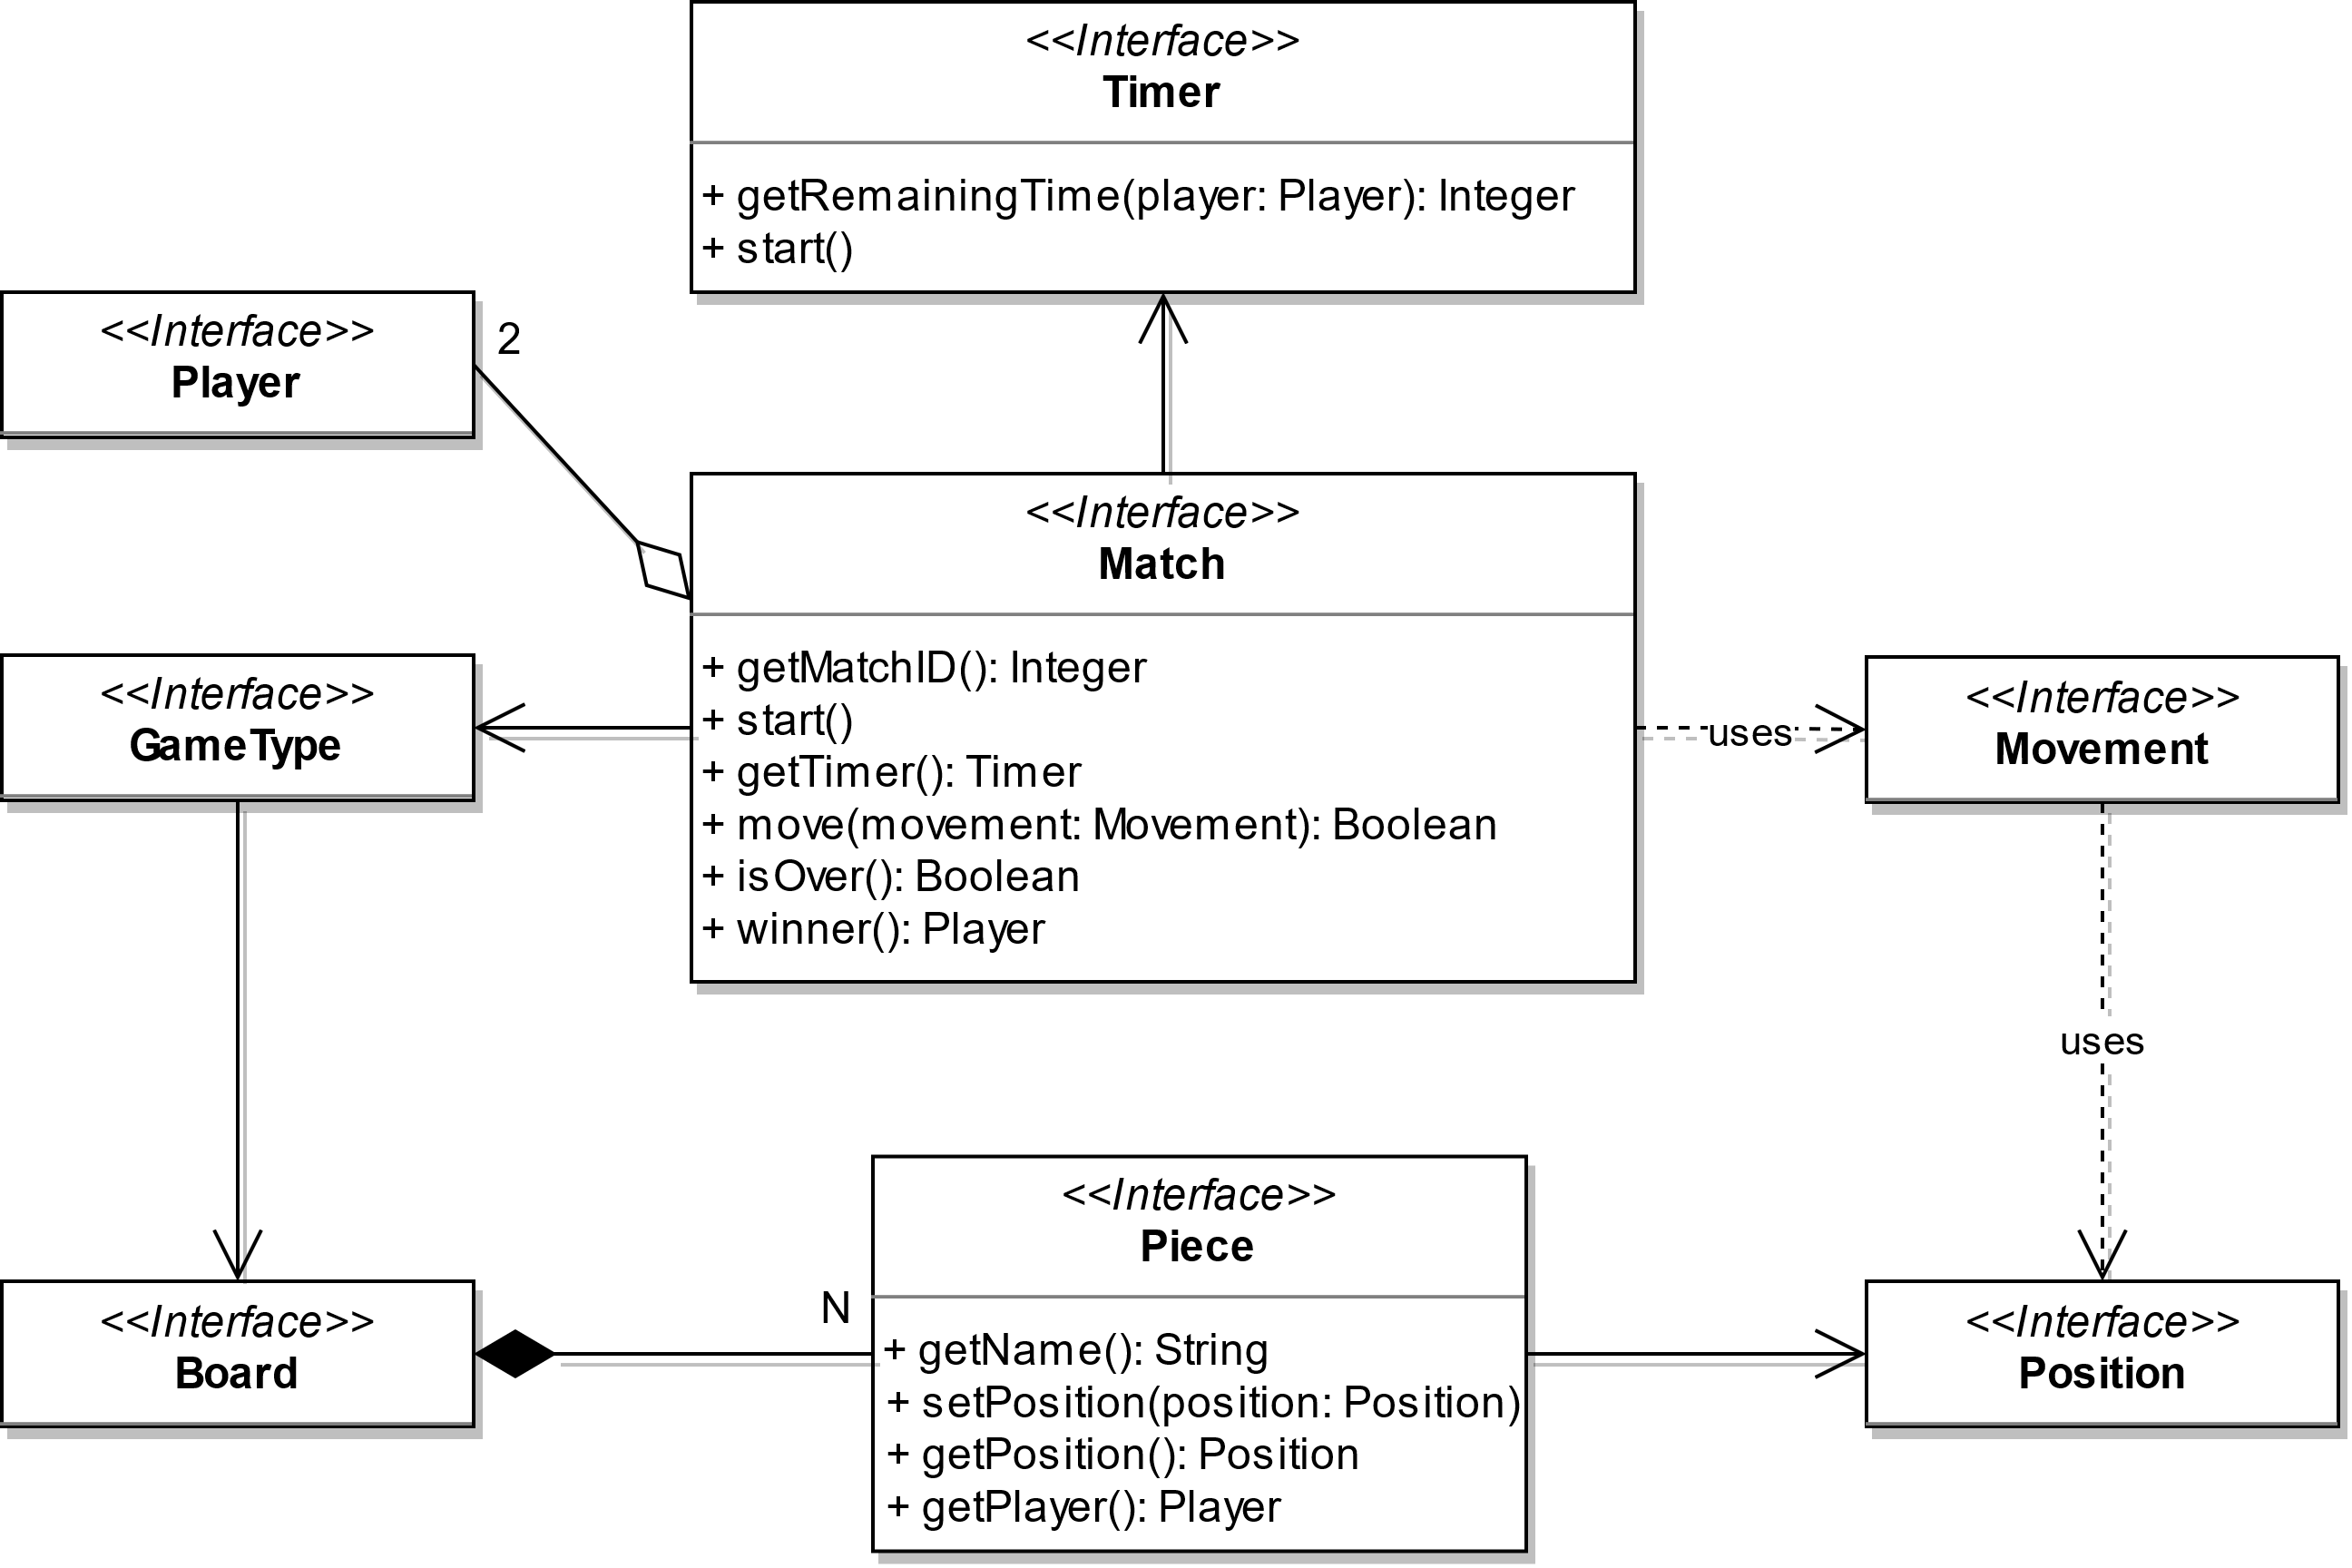
\includegraphics[width=\textwidth]{img/uml/analysis.png}
    \end{center}
    \caption{Schema UML dell'analisi del problema, con rappresentate le entità principali ed i rapporti fra loro}
    \label{img:analysis1}
\end{figure}

\chapter{Design}

\section{Architettura}

Per lo sviluppo dell'architettura di Jhaturanga si è deciso di seguire il pattern architetturale MVC (Model - View - Controller).
\\
A prova dell'estendibilità dell'applicativo dal punto di vista di MVC, abbiamo deciso di implementare anche una versione proof-of-concept da Command Line, che integra una versione basilare dell'intera applicazione seppur completamente funzionante.

\begin{figure}[H]
    \begin{center}
        \centering
        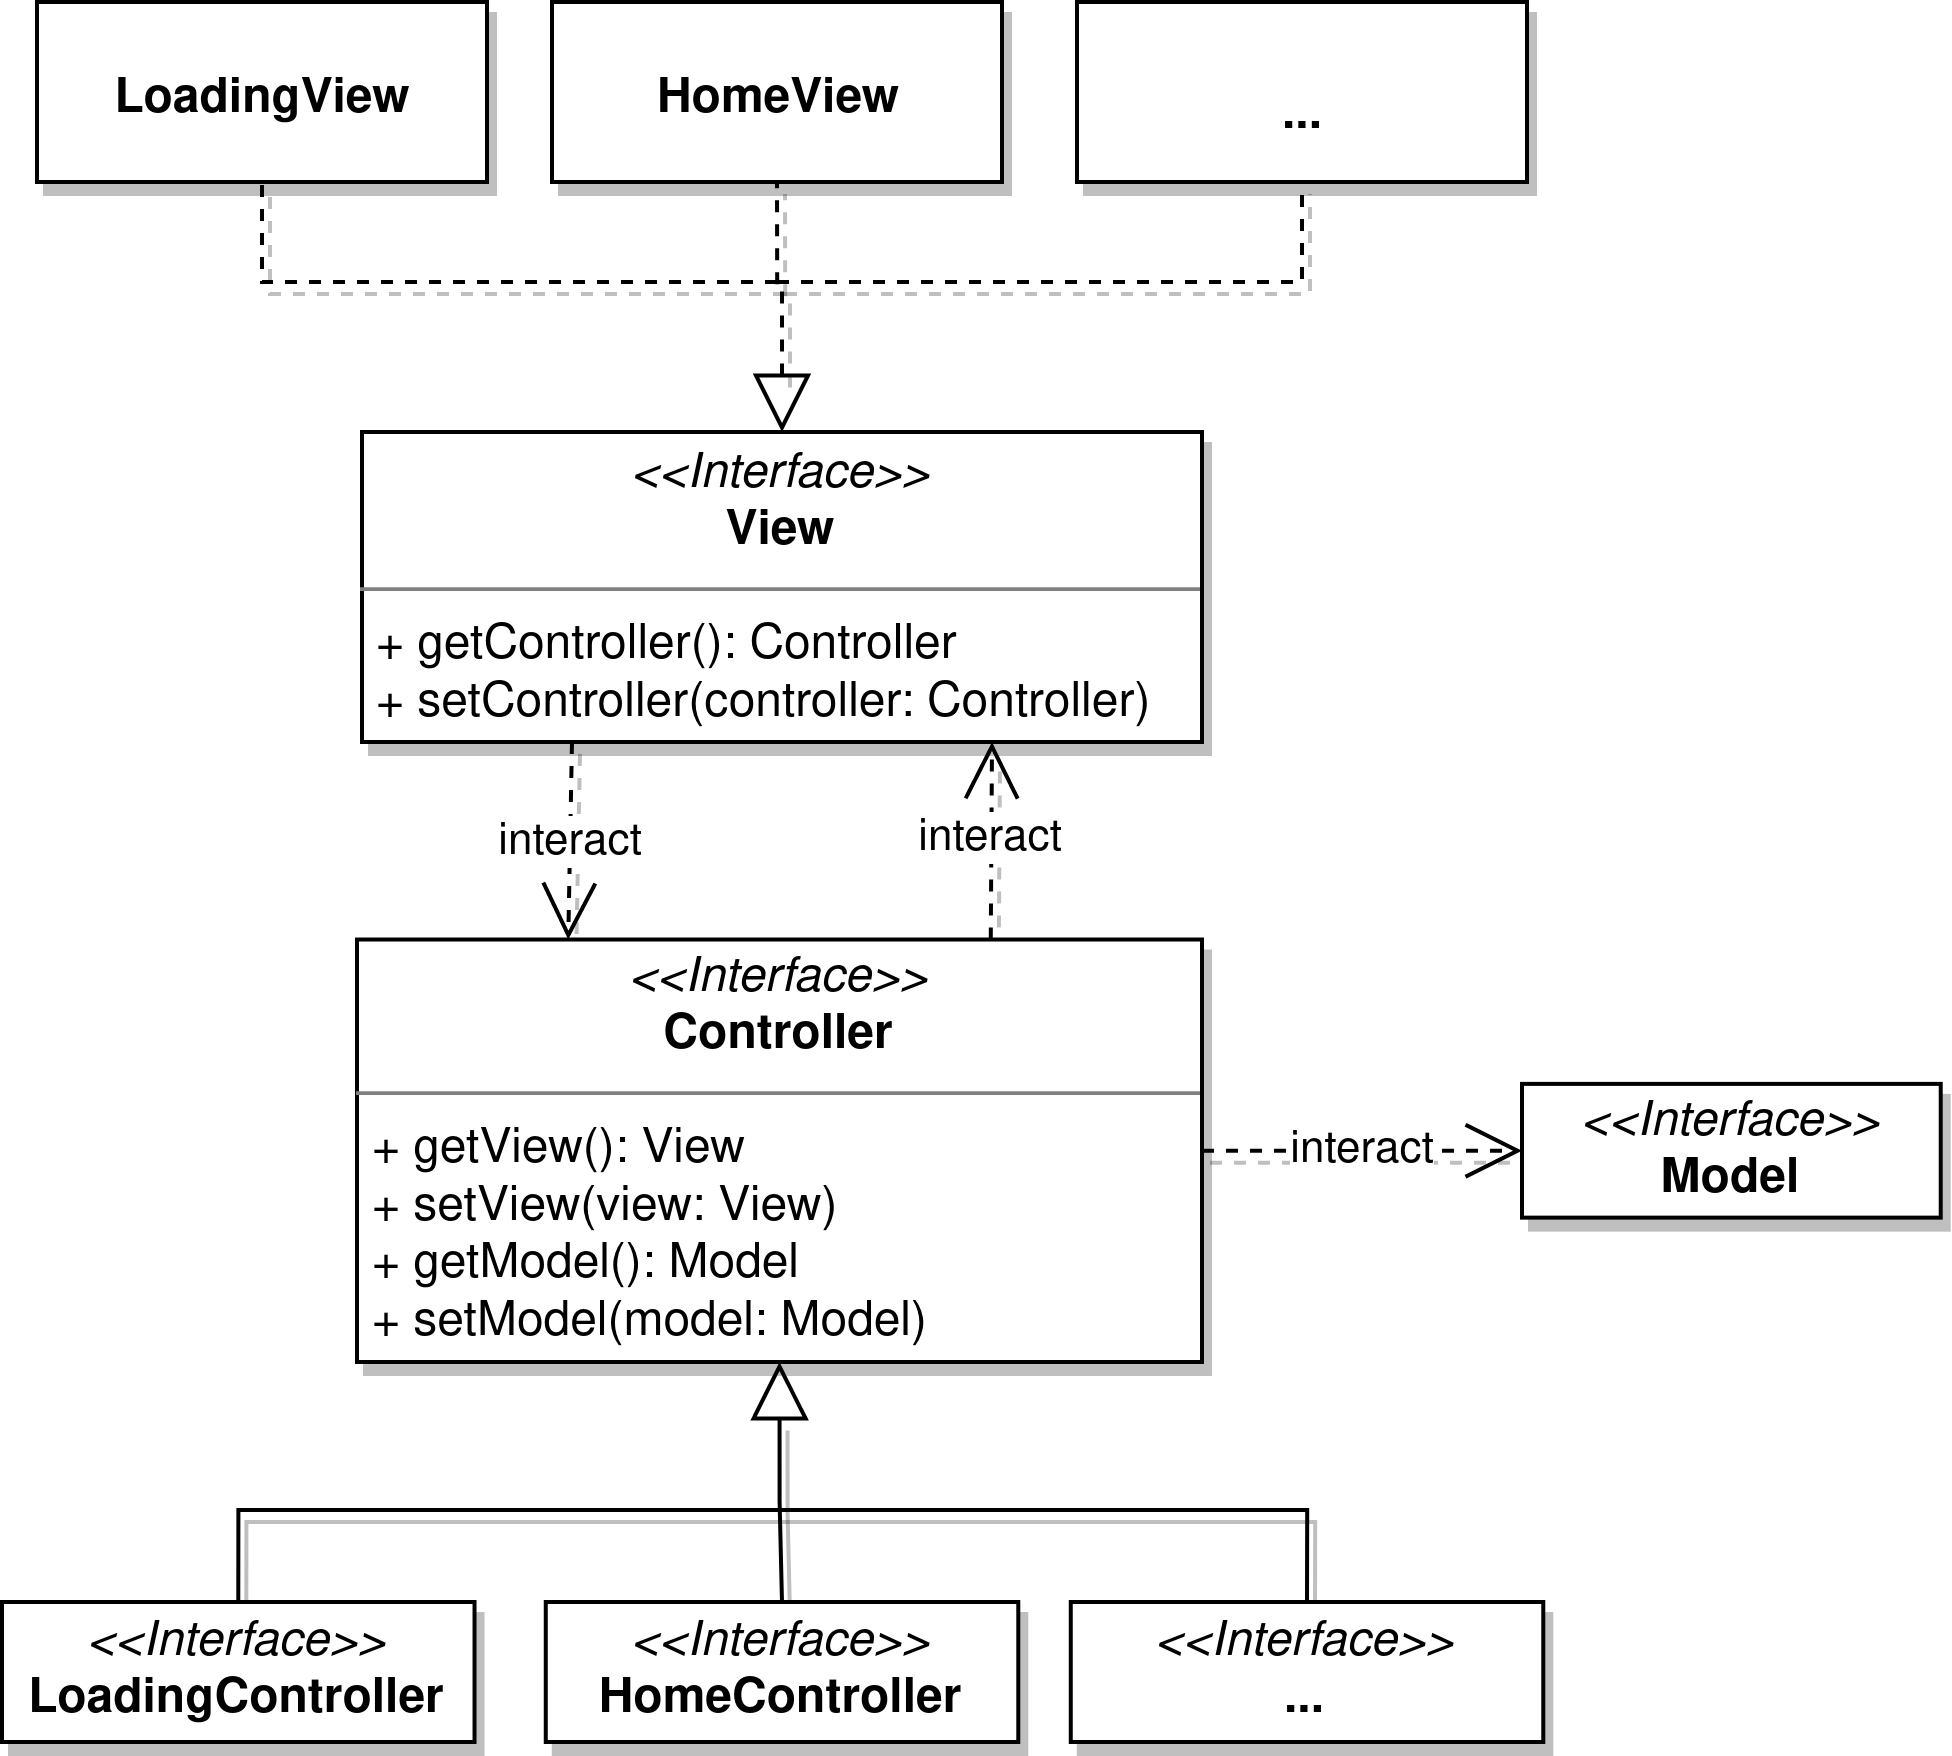
\includegraphics[scale=0.8]{img/MVC/mvc.png}
    \end{center}
    \caption{Architettura MVC da noi implementata}
    \label{img:analysis2}
\end{figure}

\subsection{Model}
Il Model si occupa di gestire le metodologie di accesso e modifica dei dati dell'applicazione e del dominio applicativo, determinando coerentemente come le interazioni dell'utente influenzino lo stato corrente dell'applicazione.\\
Scopo del model sarà quindi fornire al Controller un accesso allo stato attuale dell'applicazione.
\\
Per fornire tale funzionalità è stato scelto di utilizzare un'entità \texttt{Model}, responsabile di tenere al suo interno lo stato attuale dell'applicazione, concernente quindi i principali componenti come gli utenti e il match a cui si sta giocando.
\\
L'effettiva implementazione consiste poi nella classe \texttt{ApplicationInstance}.
\begin{figure}[H]
    \begin{center}
        \centering
        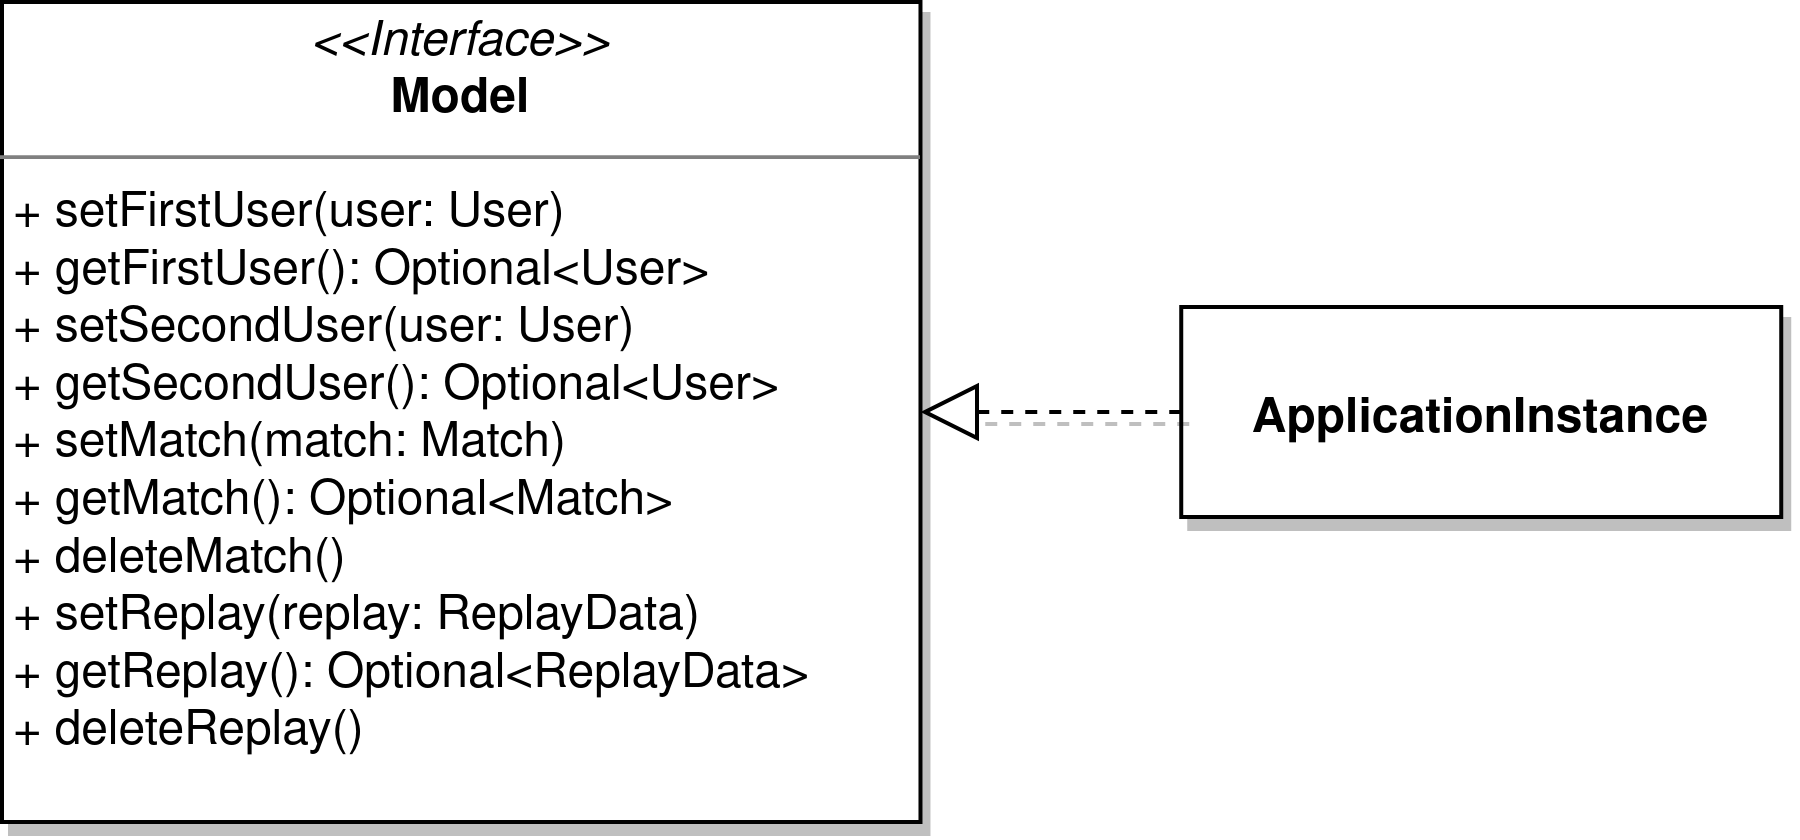
\includegraphics[width=\textwidth]{img/MVC/model.png}
    \end{center}
    \caption{Schema esemplificativo del Model}
    \label{img:analysis3}
\end{figure}

\clearpage
\subsection{View}
La \texttt{View} consiste nella schermata dell'applicazione che si occupa della gestione della parte grafica, della User Experience e dell'interazione con l'utente.
\\
É compito delle varie \texttt{View} registrare ed informare il rispettivo \texttt{Controller} di interazioni con l'applicazione da parte dell'utente, in attesa di una sua risposta sul cambiamento dei dati.
\\
Nonostante sia stato scelto sin da subito di utilizzare JavaFx, fin dalla prima fase di analisi si è deciso di strutturare la parte di \texttt{View} e \texttt{Controller} in modo indipendente dal framework utilizzato.
\\
Abbiamo quindi fatto in modo che l'entità \texttt{Controller} non sia collegata all'implementazione delle \texttt{View} come invece viene fatto quando si utilizza JavaFX che vuole un "Controller" attaccato al file fxml.
Avendo quindi isolato i \texttt{Controller} dal framework utilizzato abbiamo fatto in modo che cambiare libreria grafica implichi solamente la riscrittura della parte di \texttt{View}, lasciando invariata la parte di \texttt{Controller} e \texttt{Model}.
\\
Poichè l'applicazione è stata strutturata per avere un numero abbastanza elevato di pagine, ognuna delle quali operante su dati e parti del model differenti, si è deciso di utilizzare un' associazione 1:1 tra \texttt{View} e \texttt{Controller}.
Ovvero: ogni \texttt{View} ha associata a sè il relativo \texttt{Controller}, quest' ultimo responsabile di fornire e lavorare solamente sui dati richiesti dal contesto di quella pagina.
\
\\
É proprio grazie a quest' architettura che ci è risultato estremamente semplice e triviale sviluppare la versione da Command-Line.

\begin{figure}[H]
    \begin{center}
        \centering
        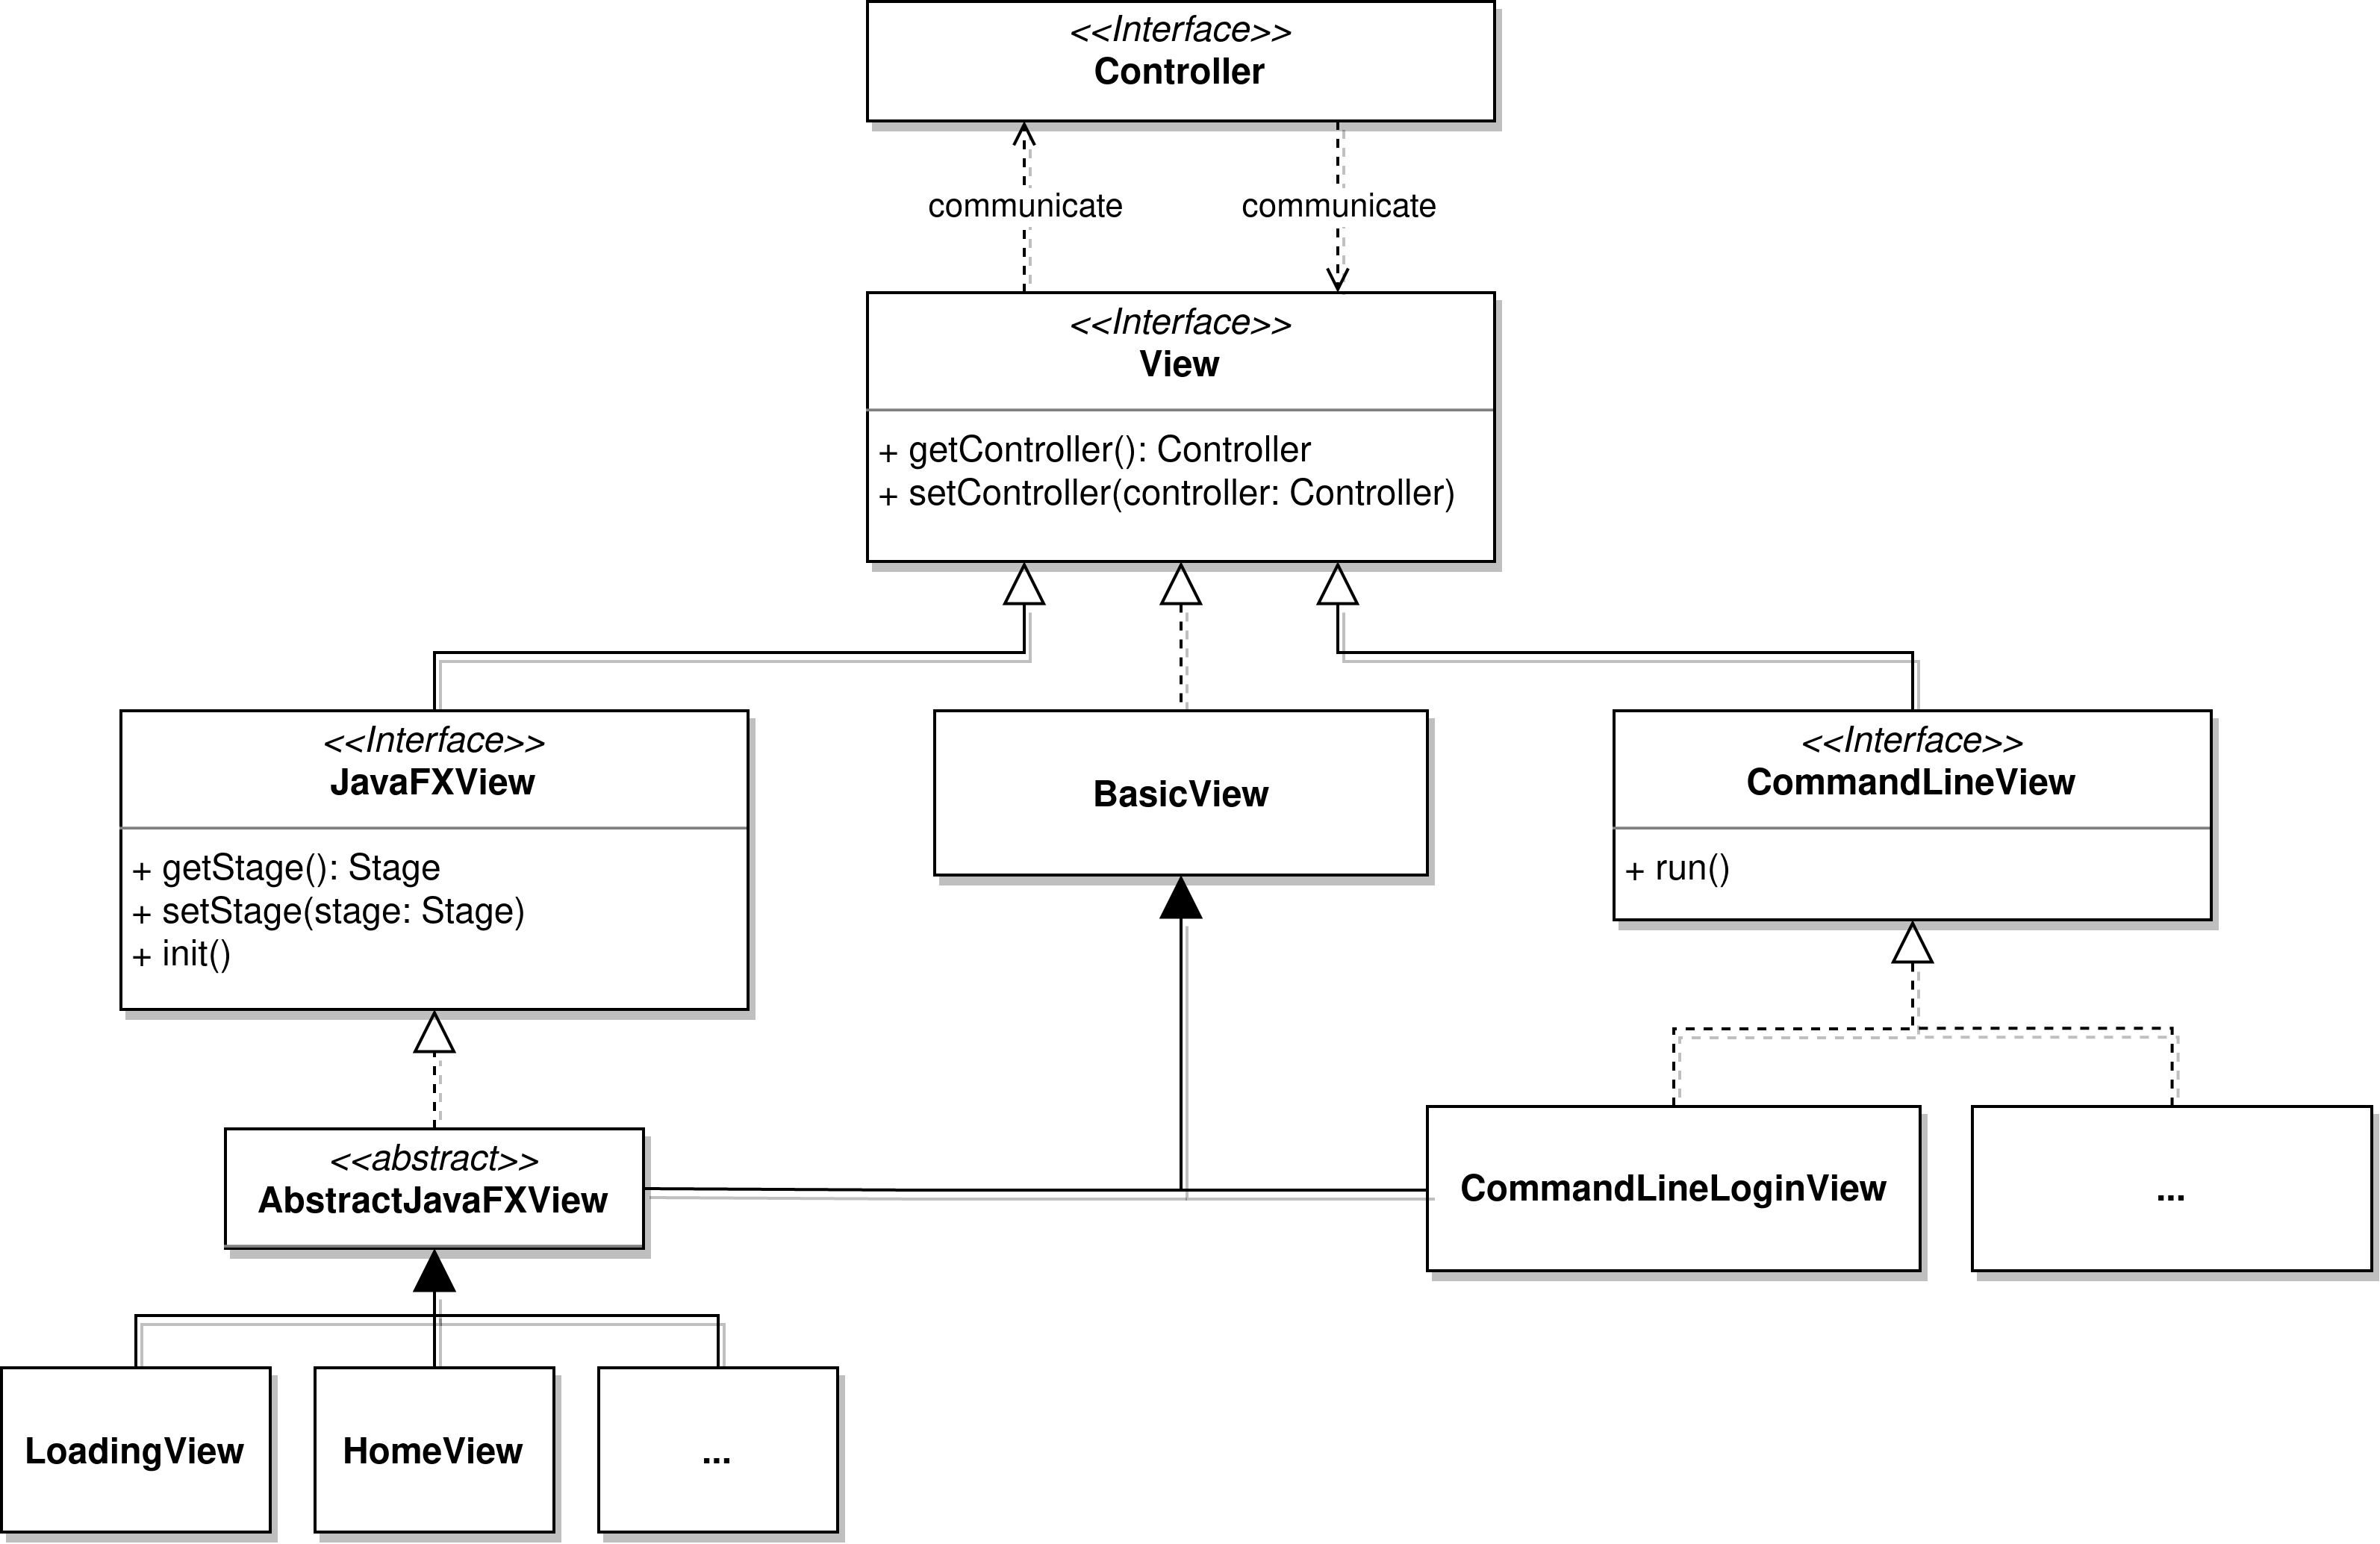
\includegraphics[width=\textwidth]{img/MVC/view.png}
    \end{center}
    \caption{Schema UML dell'architettura MVC da noi implementata}
    \label{img:analysis4}
\end{figure}

\subsection{Controller}
Il \texttt{Controller} è quella componente cui spetta gestire in maniera conseguenziale le interazioni da parte dell'utente nella \texttt{View}, comunicando quindi al \texttt{Model} il cambiamento avvenuto.
\\
Una volta che il \texttt{Model} avrà completato l'elaborazione della richiesta di cambiamento, il \texttt{Controller} avviserà la propria \texttt{View}, in modo tale che quest'ultima possa aggiornarsi in maniera coerente secondo le regole specificate dal \texttt{Model}.
\\
Come già accennato nella sezione precedente, si è scelto di evitare l'utilizzo di un singolo controller, sia per i motivi sopracitati, sia perché un unico controller sarebbe risultato essere una "God Class", avente un eccessivo grado di responsabilità.
\\
Abbiamo deciso quindi di organizzare anche il lato controller secondo una struttura gerarchica, dove l'entità del \texttt{Controller} è rappresentata dall'interfaccia che ne incapsula il funzionamento, ossia avere l'accesso al \texttt{Model} e alla \texttt{View}.
\\
Da questo derivano poi le varie specializzazioni dei vari \texttt{Controller}, ognuno specifico secondo il contratto delle funzionalità, determinanti queste quali parti del \texttt{Model} concernono gli accessi del suddetto.
\begin{figure}[H]
    \begin{center}
        \centering
        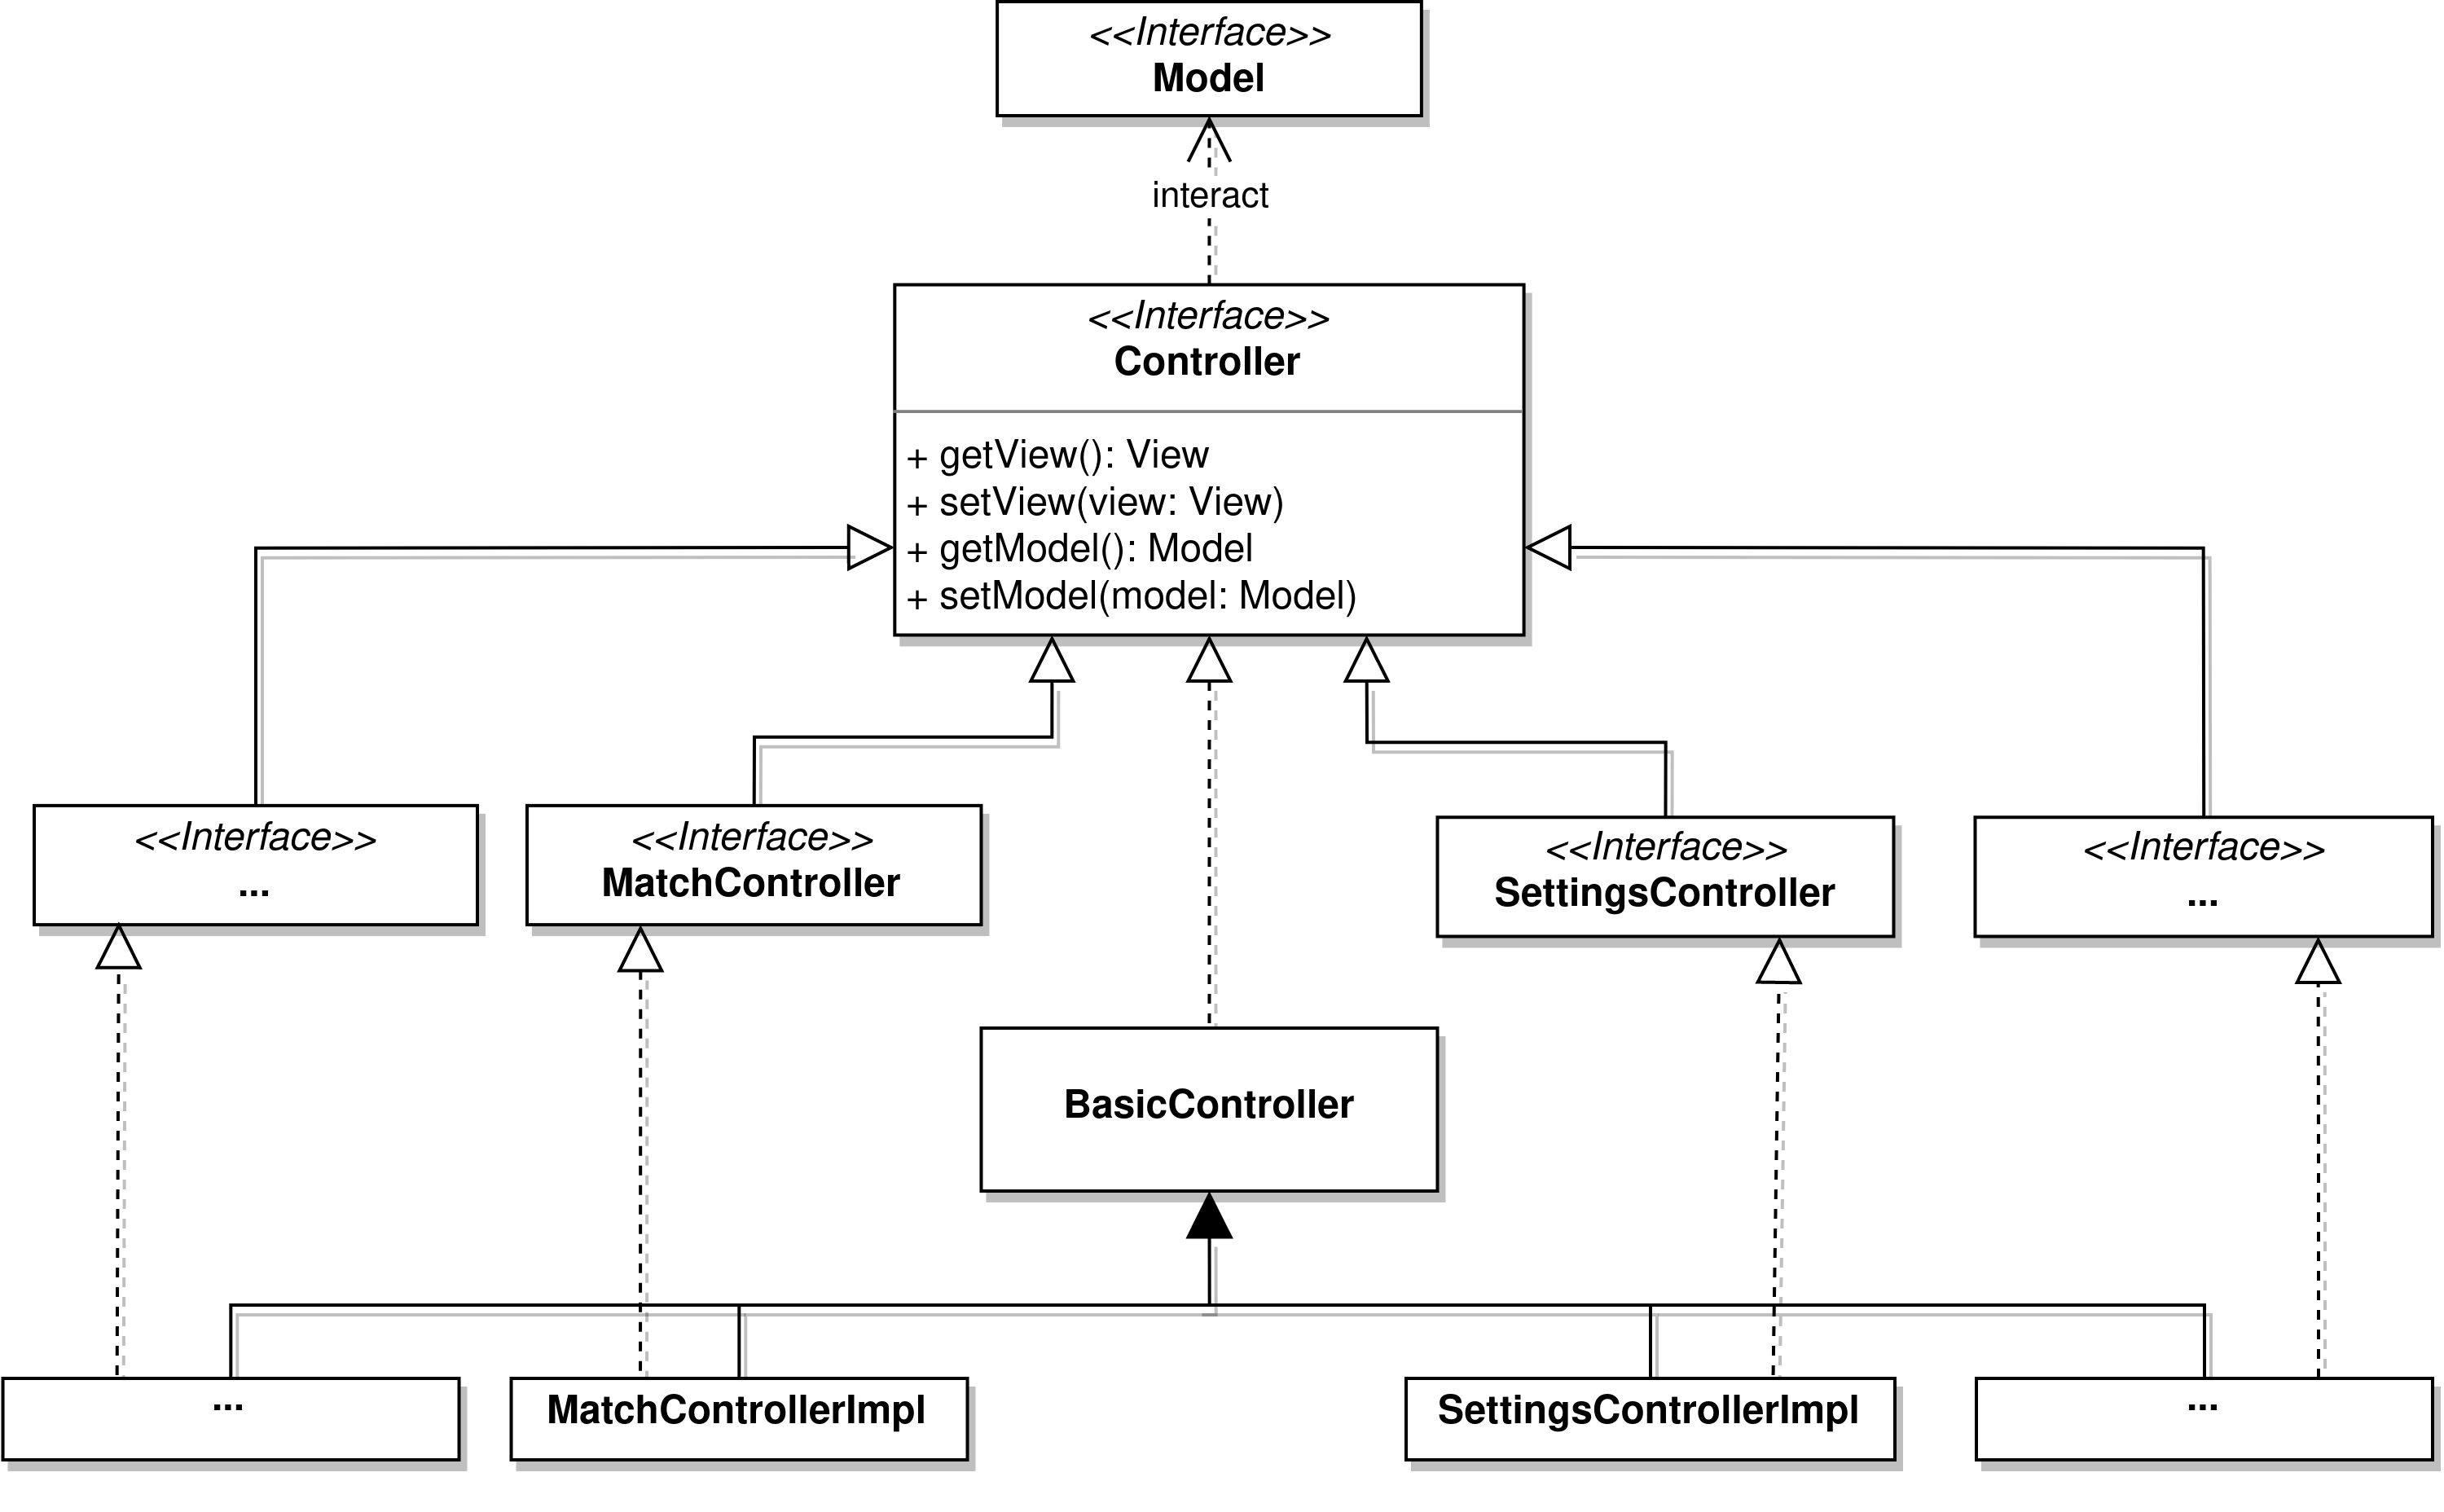
\includegraphics[width=\textwidth]{img/MVC/controller.png}
    \end{center}
    \caption{Organizzazione dei \texttt{Controller} nell'architettura MVC}
    \label{img:analysis5}
\end{figure}

\paragraph{}
\
\\
Quello che ne è derivato è stata un architettura dell'applicazione con un alto livello di estendibilità, che ha agevolato di molto lo sviluppo, poiché ogni pagina e rispettivo \texttt{Controller} potevano lavorare indipendentemente dalle altre coppie \texttt{View}-\texttt{Controller}, rendendo possibile, e soprattutto molto semplice, integrare nuove funzionalità.

\clearpage
\section{Design dettagliato}

\subsection{Andruccioli Manuel}

Fin dalla fase di analisi, miravamo ad avere un'applicazione con la possibilità di mantenere i dati relativi ai risultati delle partite dei giocatori, per poi poterli visualizzare successivamente.
\\
La parte della quale mi sono occupato maggiormente è stata la realizzazione di un sotto sistema per la memorizzazione persistente dei dati, il recupero di essi e la possibilità di riorganizzarli attraverso un classifica.

\subsubsection*{User}
\label{User}

A fronte di un'accurata analisi, si è deciso di separare l'entità User da \texttt{\nameref{Player}}, trattando quest'ultima in una sezione apposita.
\\
Lo scopo principale di \textbf{User} è quello di incapsulare l'utente che si autentica, per poi tener traccia dei risultati delle partite (vittoria, sconfitta o pareggio).
\\
Per le funzionalità basilari che dobbiamo offrire, ho deciso di rendere univoco lo username dell'utente, che verrà riservato durante la registrazione e, in coppia con la password inserita, serviranno per potersi autenticare successivamente.
\\
Per la creazione degli Users ho deciso di adottare il pattern \textbf{Builder}, per avere la possibilità di spezzare le fasi di creazione se necessario. Attualmente User contiene poche informazioni, ma se in futuro si vorranno aggiungere responsabilità, questa entità, così facendo, sarà facilmente scalabile. Inoltre ho pensato che questa procedura di creazione potrebbe tornale utile nel caso in cui si voglia generare giocatori fittizi, con dati random, nelle partite contro il computer.

% User image
\begin{figure}[ht]
    \begin{center}
        \centering
        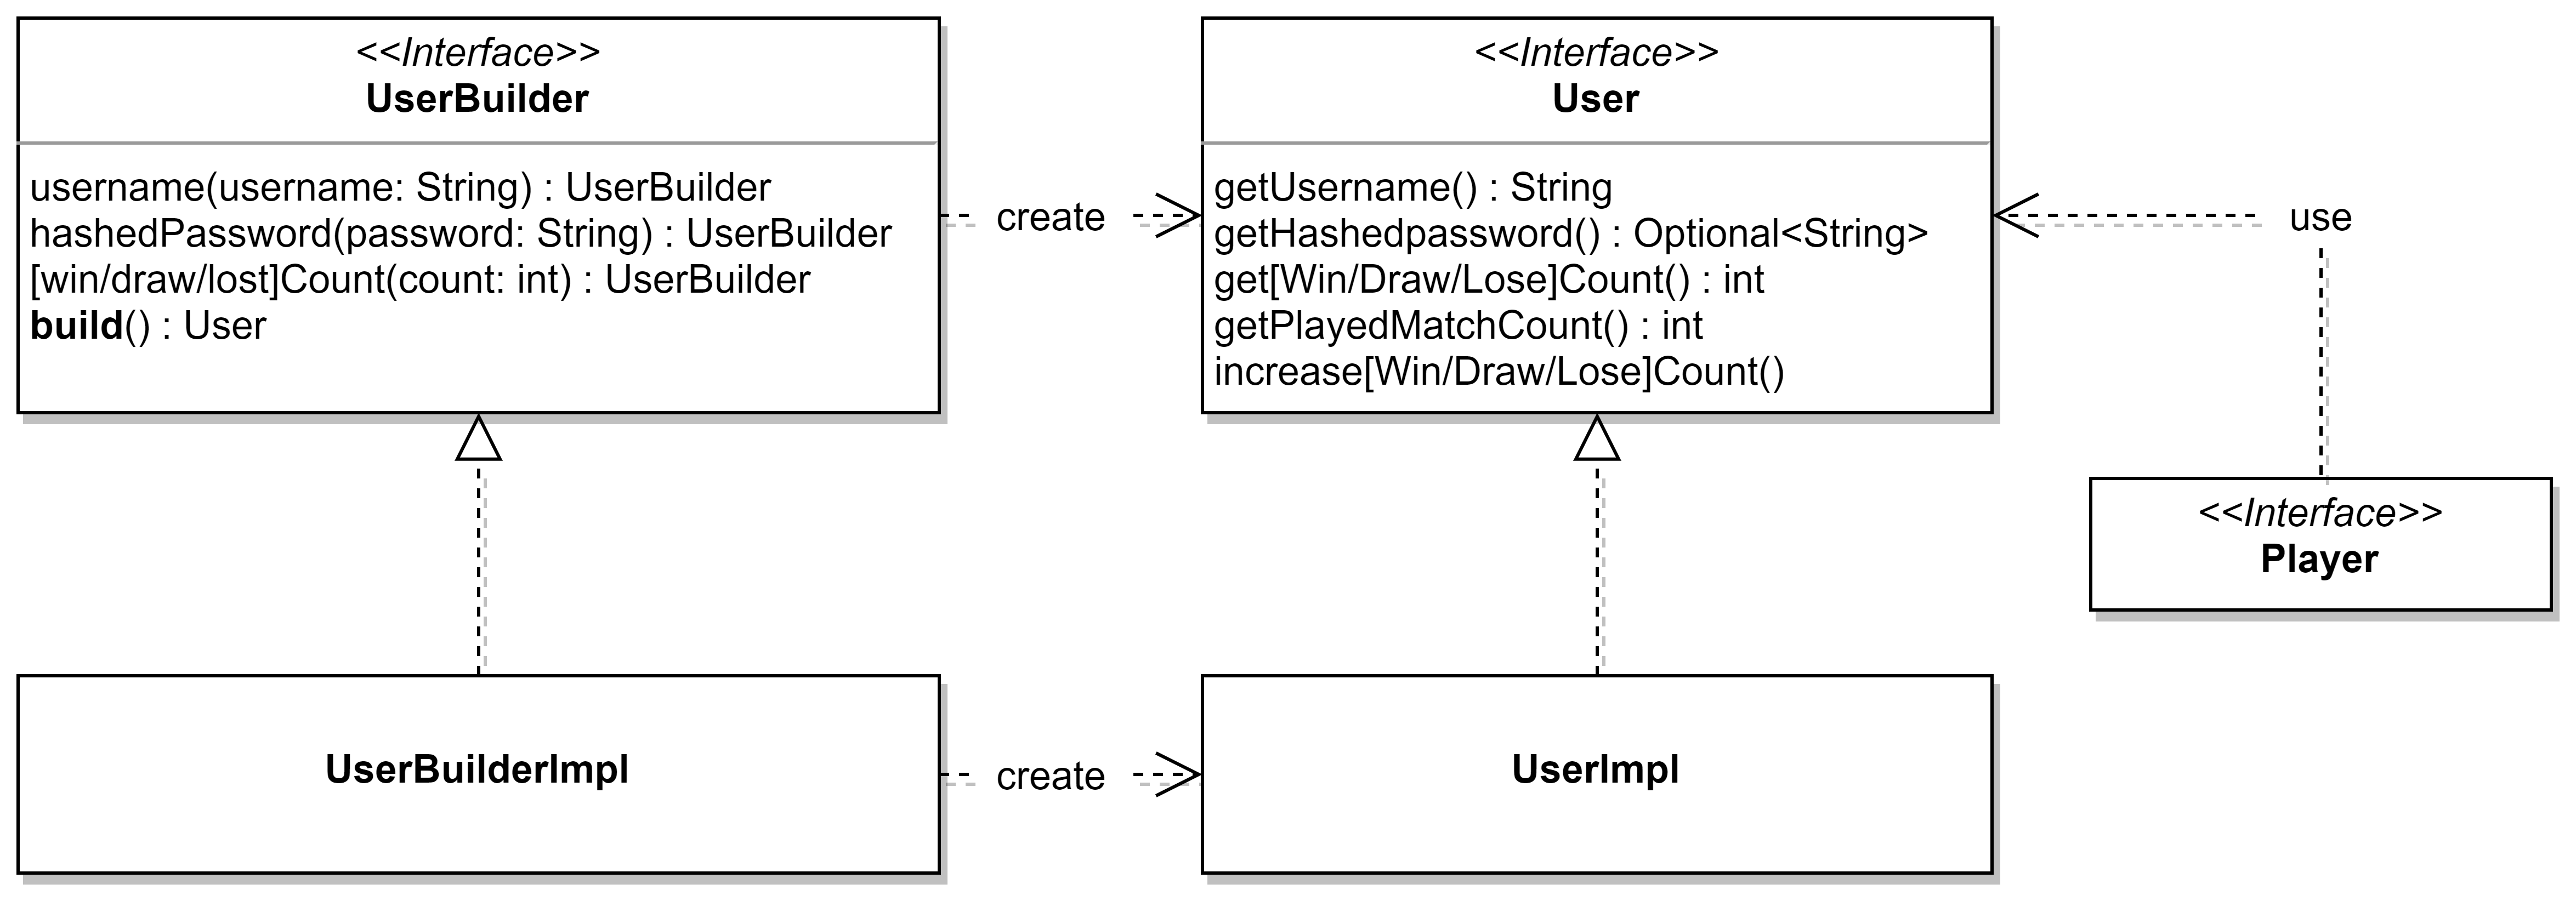
\includegraphics[width=\textwidth]{img/Manuel/shadow/User.png}
    \end{center}
    \caption{User e creazione}
    \label{img:User}
\end{figure}
%

\subsubsection*{Function Concatenator}

Dovendo richiedere dati all'utente per inserire username e password, ho ideato questa interfaccia per facilitare ed estendere, il controllo su di essi ed ottenere un determinato risultato al termine dei test proposti.
\\
L'intento principale è quello di avere la possibilità di concatenare tra loro funzioni dello stesso tipo, per poi generarne una nuova. Entrambe le operazioni non sono determinate, demandando il comportamento proprio alle implementazioni, realizzando ciò di cui si ha necessità.
\\
Infatti, ho realizzato \texttt{StringValidatorImpl} che si occupa di concatenare test (funzioni che accettano una Stringa e restituiscono un risultato), per poi restituire una nuova funzione, costruita sulla base di ciò che è stato fornito. Come risultato ho voluto utilizzare una \texttt{enum}, aggiungendo un messaggio esplicativo.
\\
Per facilitare la creazione, ho disposto una classe che contiene alcune funzioni di test già implementate.
\\
Una volta creata la funzione validatrice, basterà applicarla ad una stringa, ottenendo come risultato \texttt{'CORRECT'} se passa tutti i test, oppure il primo risultato di errore.
\\
Questo approccio utilizzato, secondo me, è facilmente estendibile e/o modificabile, andando ad agire o creando nuovi test.

% Function Concatenator
\begin{figure}[ht]
    \begin{center}
        \centering
        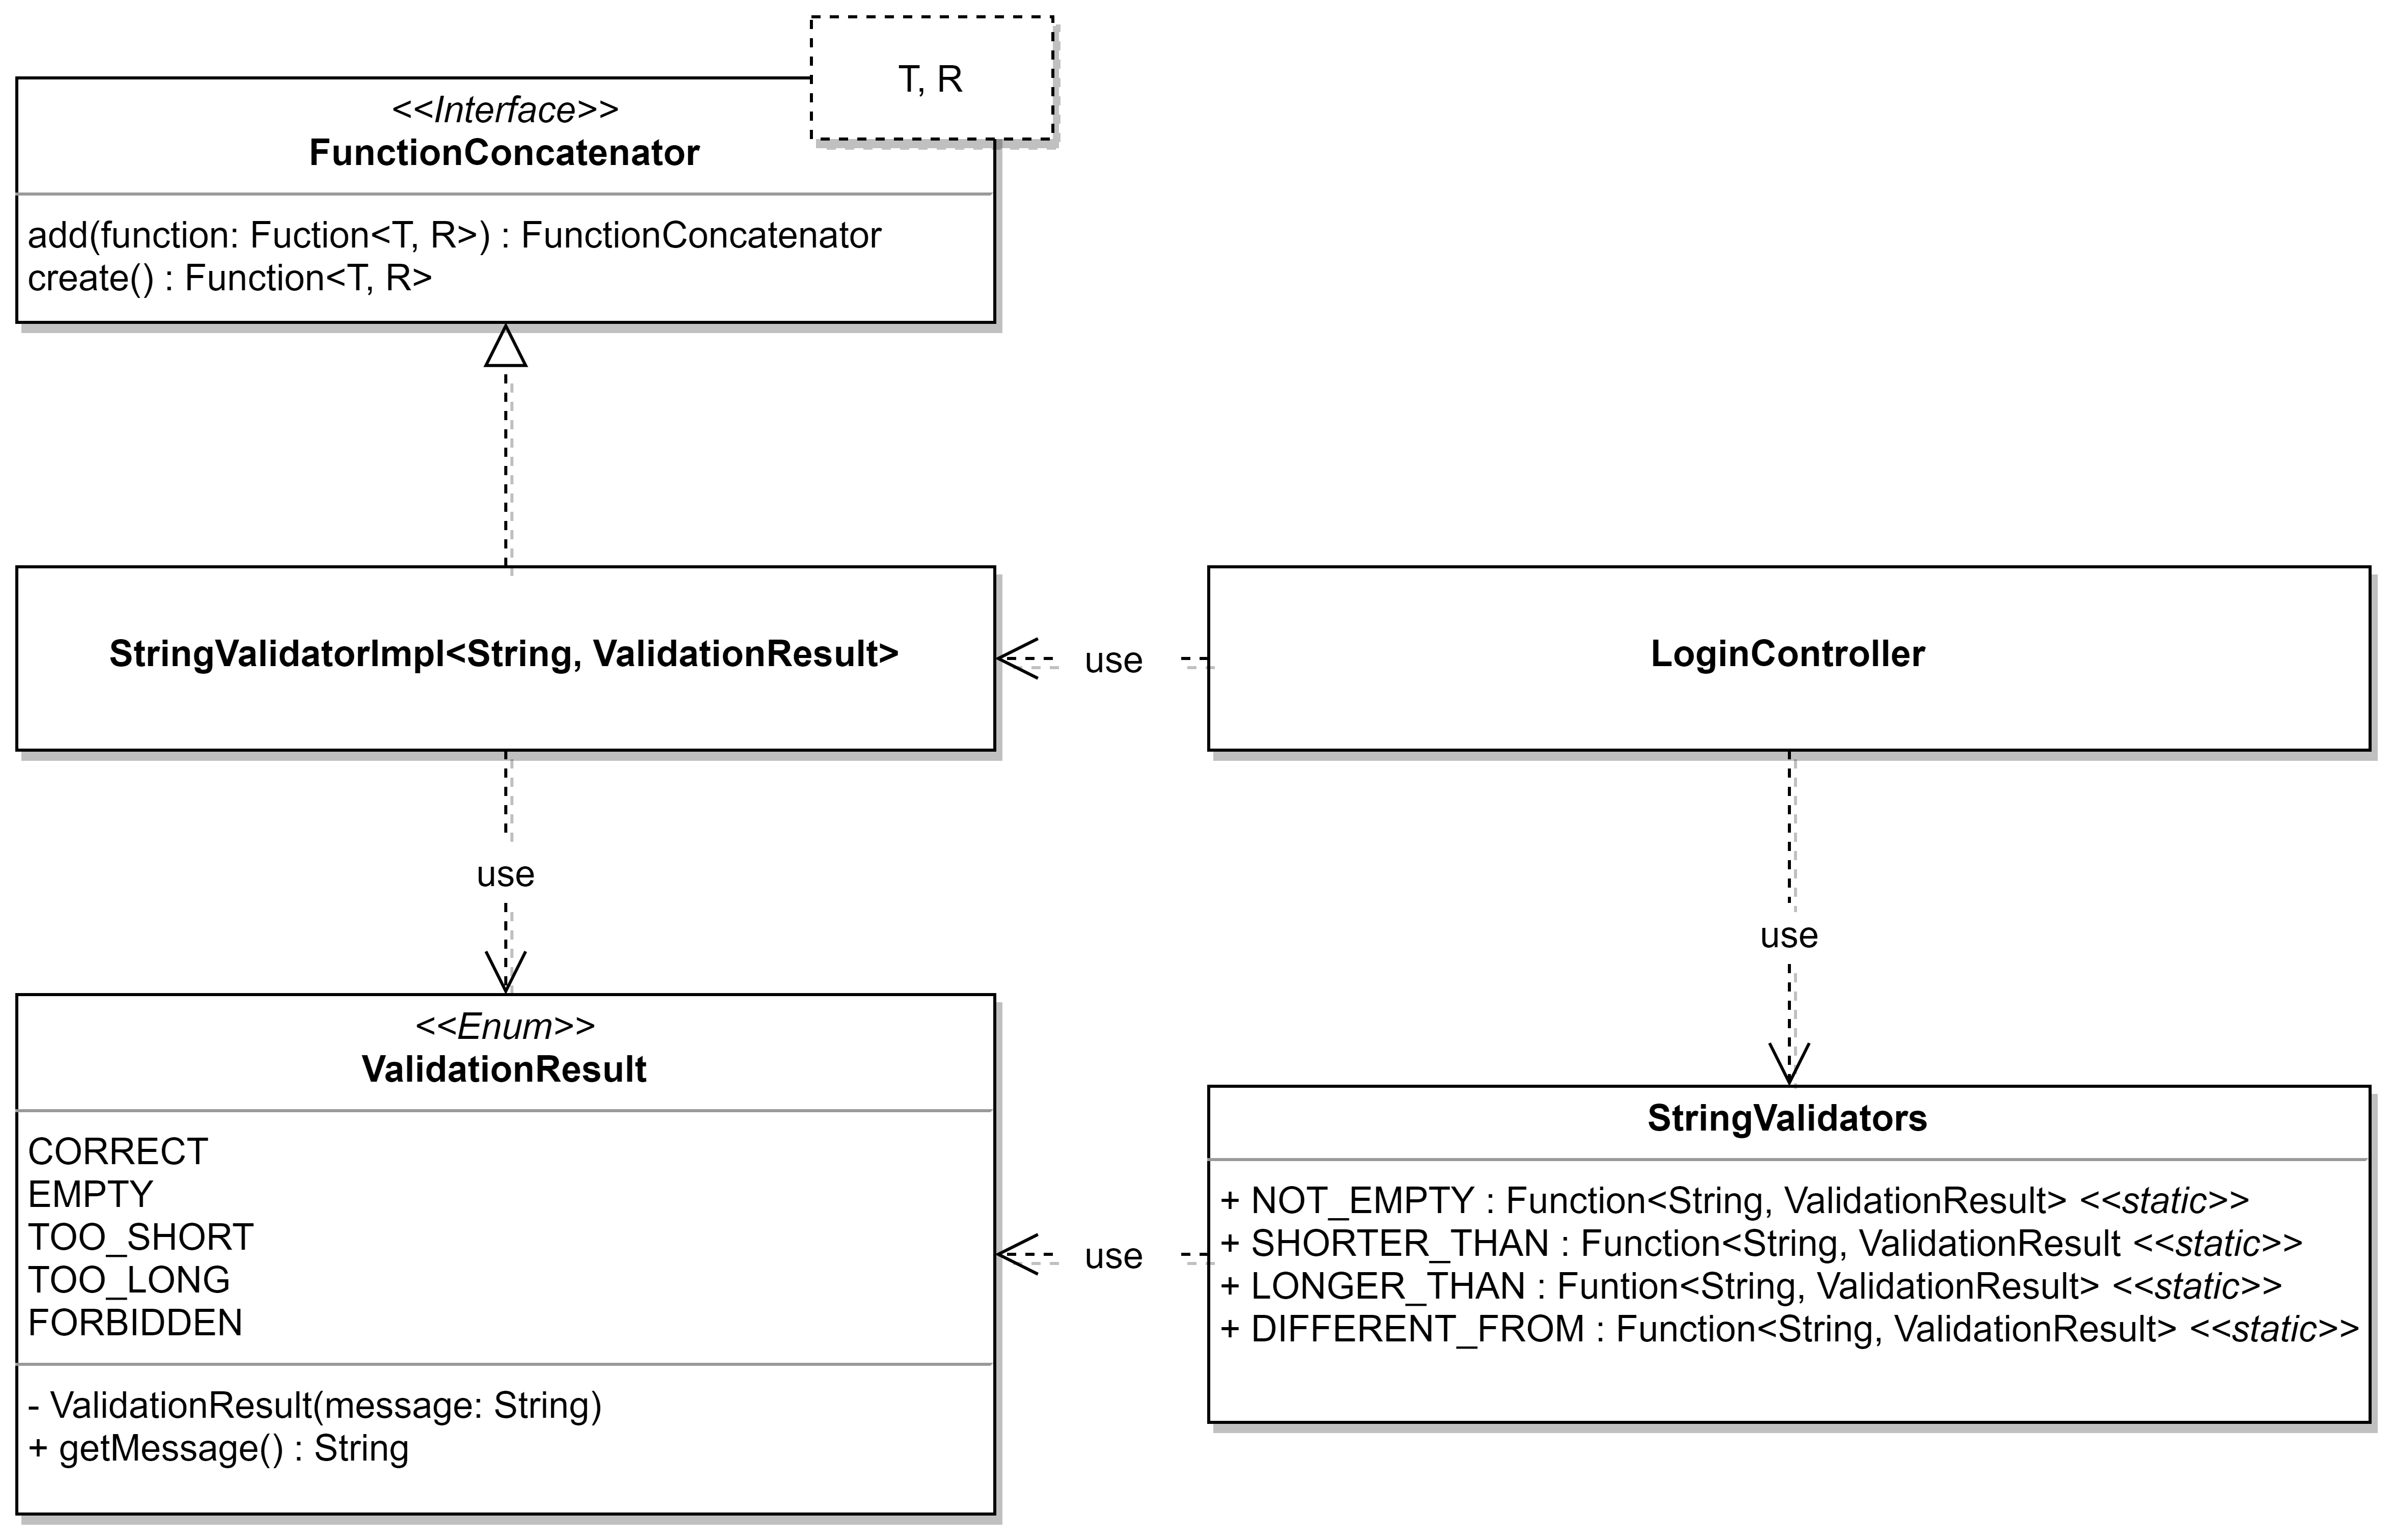
\includegraphics[width=\textwidth]{img/Manuel/shadow/FunctionConcatenator.png}
    \end{center}
    \caption{Concatenatore di funzioni}
    \label{img:FunctionConcatenator}
\end{figure}
%

\subsubsection*{User Manager}
\label{UserManager}

Nel momento in cui è giunta la necessità di salvare i dati degli utenti in una memoria persistente, ho realizzato fosse corretto separare le responsabilità delle varie parti in gioco, per poter riutilizzare il codice.
\\
Da questa premessa infatti, ho realizzato lo \texttt{UserManager}, un'interfaccia che stabilisce le varie operazioni fattibili sulla collezione di utenti dell'applicazione. Avrei potuto implementare qua dentro direttamente il salvataggio e recupero dei dati su file, ma non sarebbe stato molto estendibile.
\\
Così facendo, ho deciso di adottare il pattern \textbf{Strategy}: l'implementazione riceve una strategia mediante il costruttore, per salvare i dati, della quale si compone e delega ad essa le varie operazioni di I/O.
\\
La \texttt{UsersDataStorageStrategy} difatti, sancisce le operazioni eseguibili sui dati in memoria persistente, implementando gli opportuni meccanismi, ad esempio, per andare a legge e scrivere su file. Questo grado di libertà infatti, permette di modificare facilmente il metodo di archiviazione, scrivendo una nuova strategia. Ad esempio è possibile scrivere su file di testo, utilizzare uno stream di byte, ma anche impiegare un database. Io ho realizzato una semplice JsonStrategy, che sfrutta per l'appunto il formato JSON.

% User Manager
\begin{figure}[ht]
    \begin{center}
        \centering
        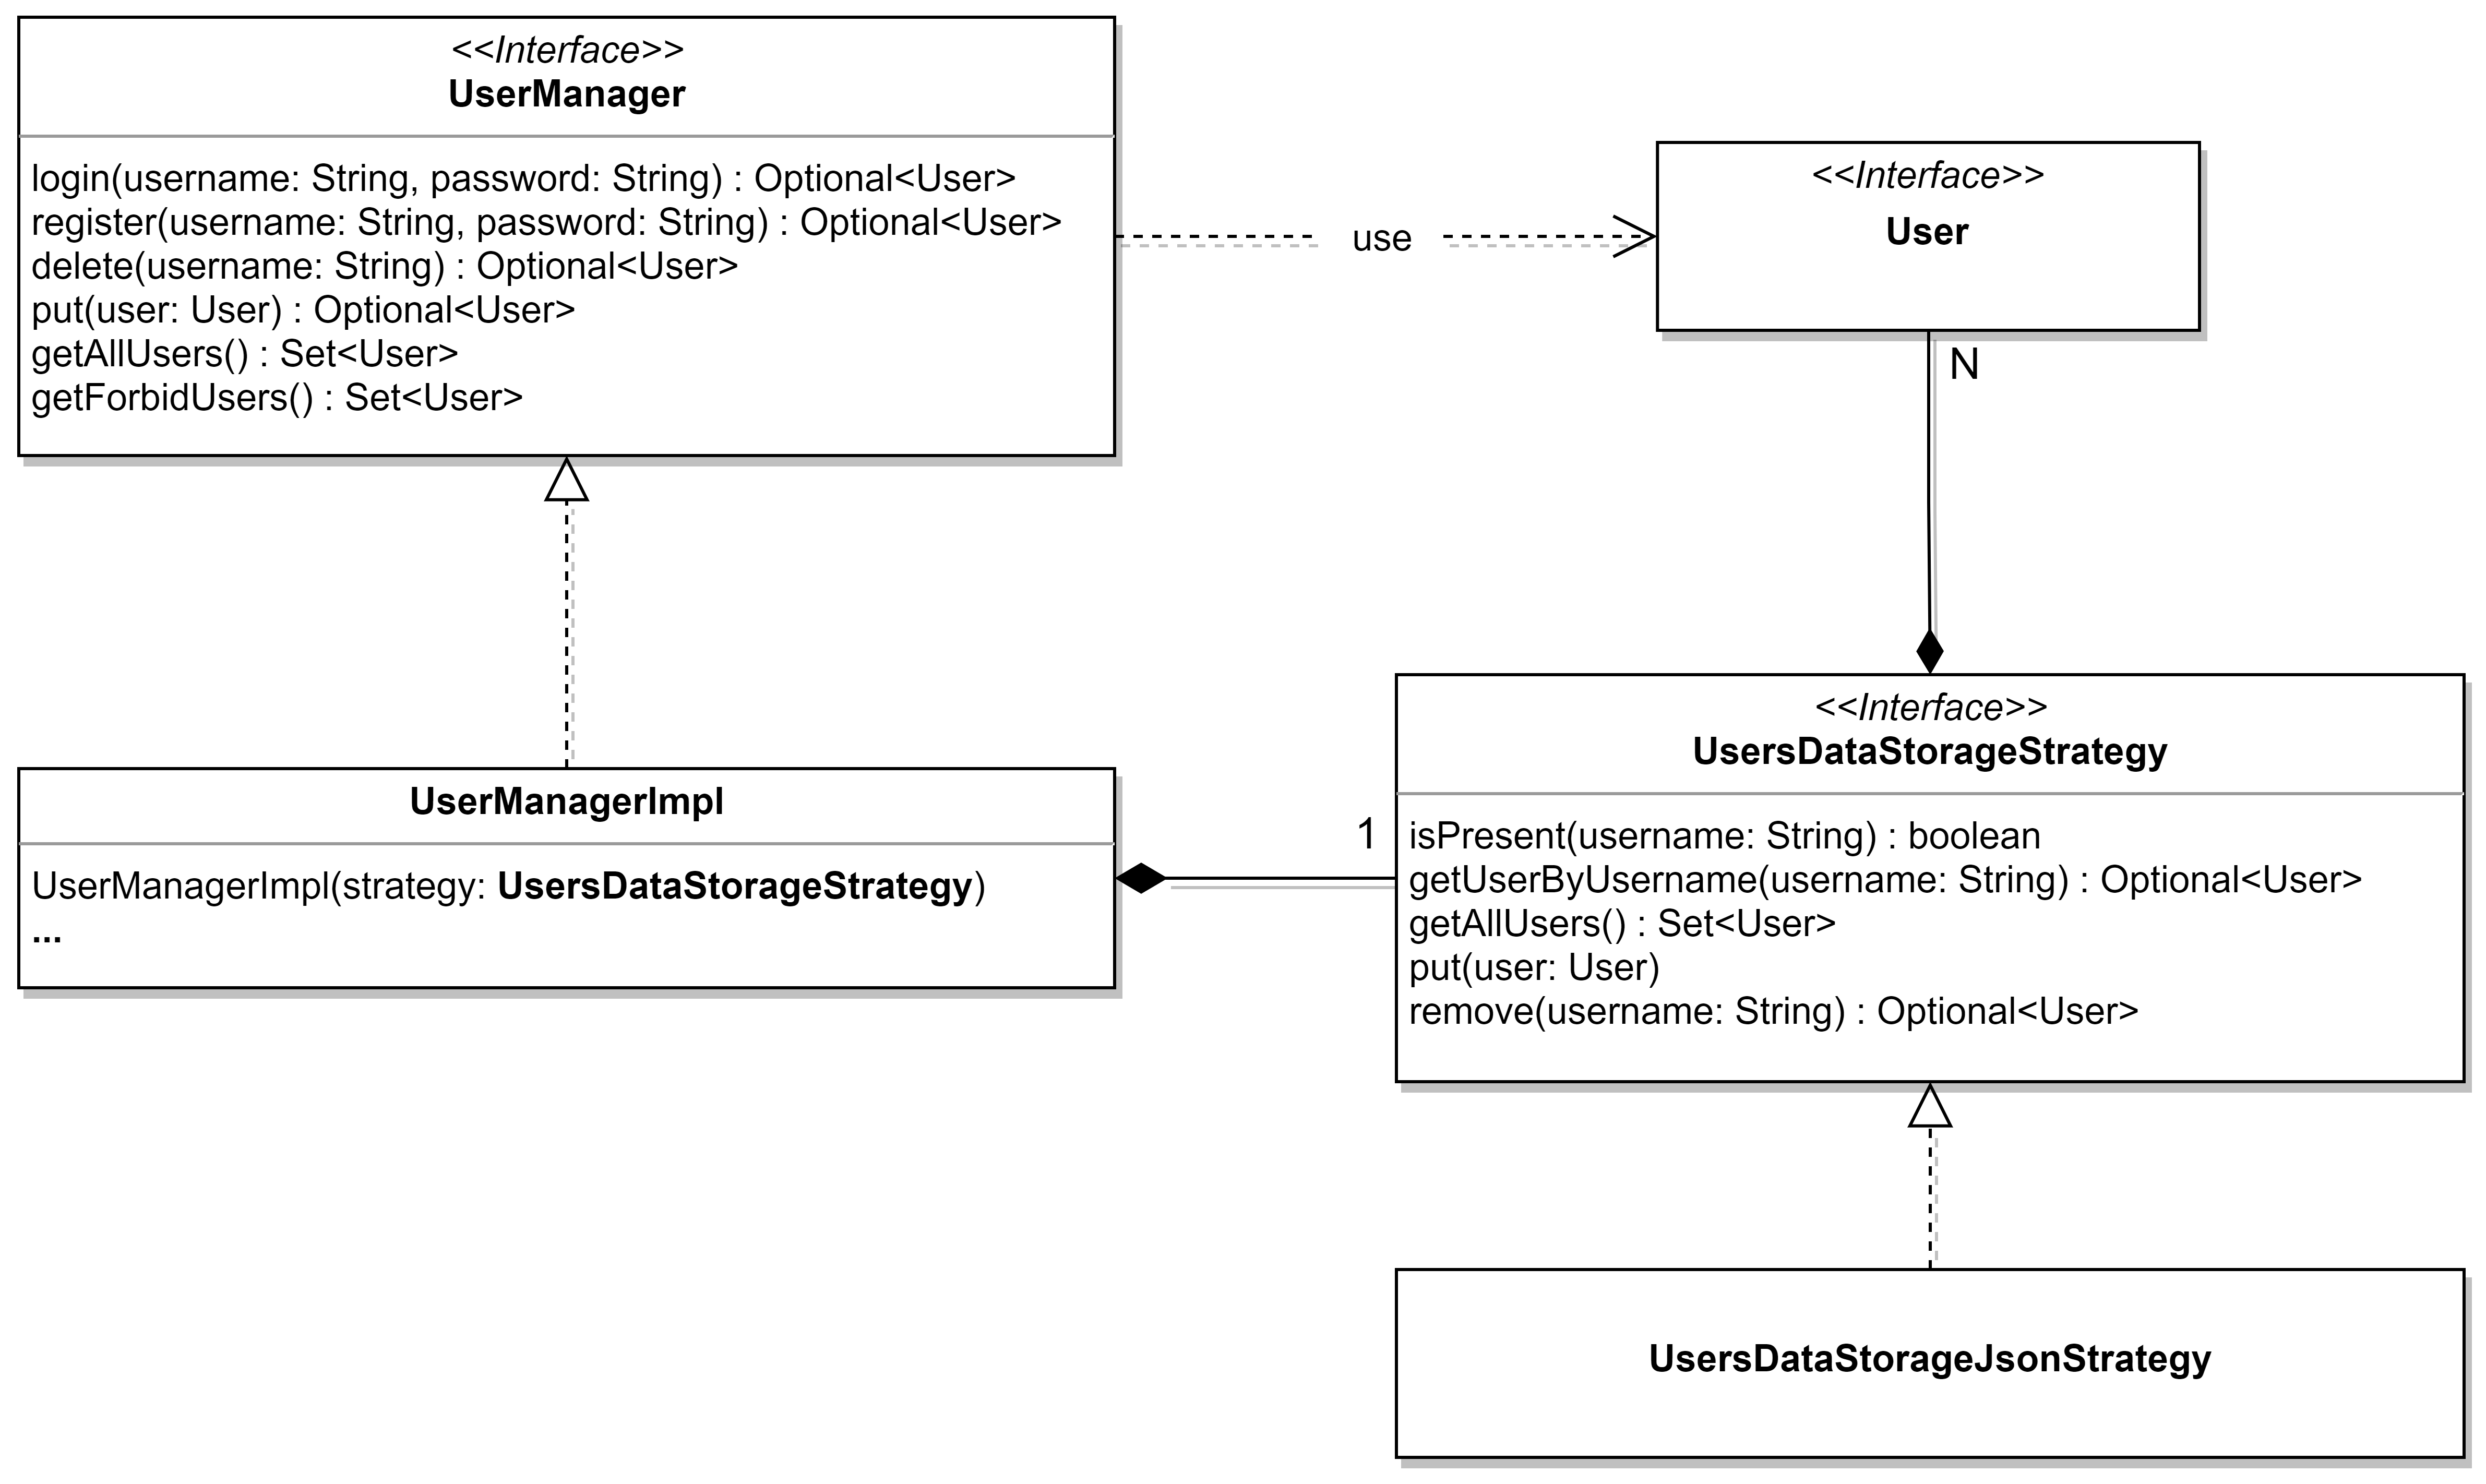
\includegraphics[width=\textwidth]{img/Manuel/shadow/UserManager.png}
    \end{center}
    \caption{User Manager per gli utenti dell'applicazione}
    \label{img:UserManager}
\end{figure}
%

\subsubsection*{Accesso unificato allo User Manager}

Dopo la realizzazione dello \texttt{\nameref{UserManager}} si sarebbe potuto verificare un inconveniente non da poco. Nel caso in cui si scrivessero più strategie, non comunicanti tra di loro (e.g. salvano gli utenti su due file diversi), si avrebbe una frammentazione dei dati, che comprometterebbe la veridicità degli stessi. 
\\
Proprio per questo motivo, ho deciso di adottare il pattern \textbf{Singleton}, per rendere unico nell'applicazione, l'accesso allo User Manager. Così facendo posso ovviare ai problemi riportati sopra, senza però limitare la struttura precedentemente realizzata. Infatti, nel caso in cui si voglia cambiare la strategia di salvataggio, basterà modificare all'interno di \texttt{UserManagerSingleton}.

% Singleton
\begin{figure}[ht]
    \begin{center}
        \centering
        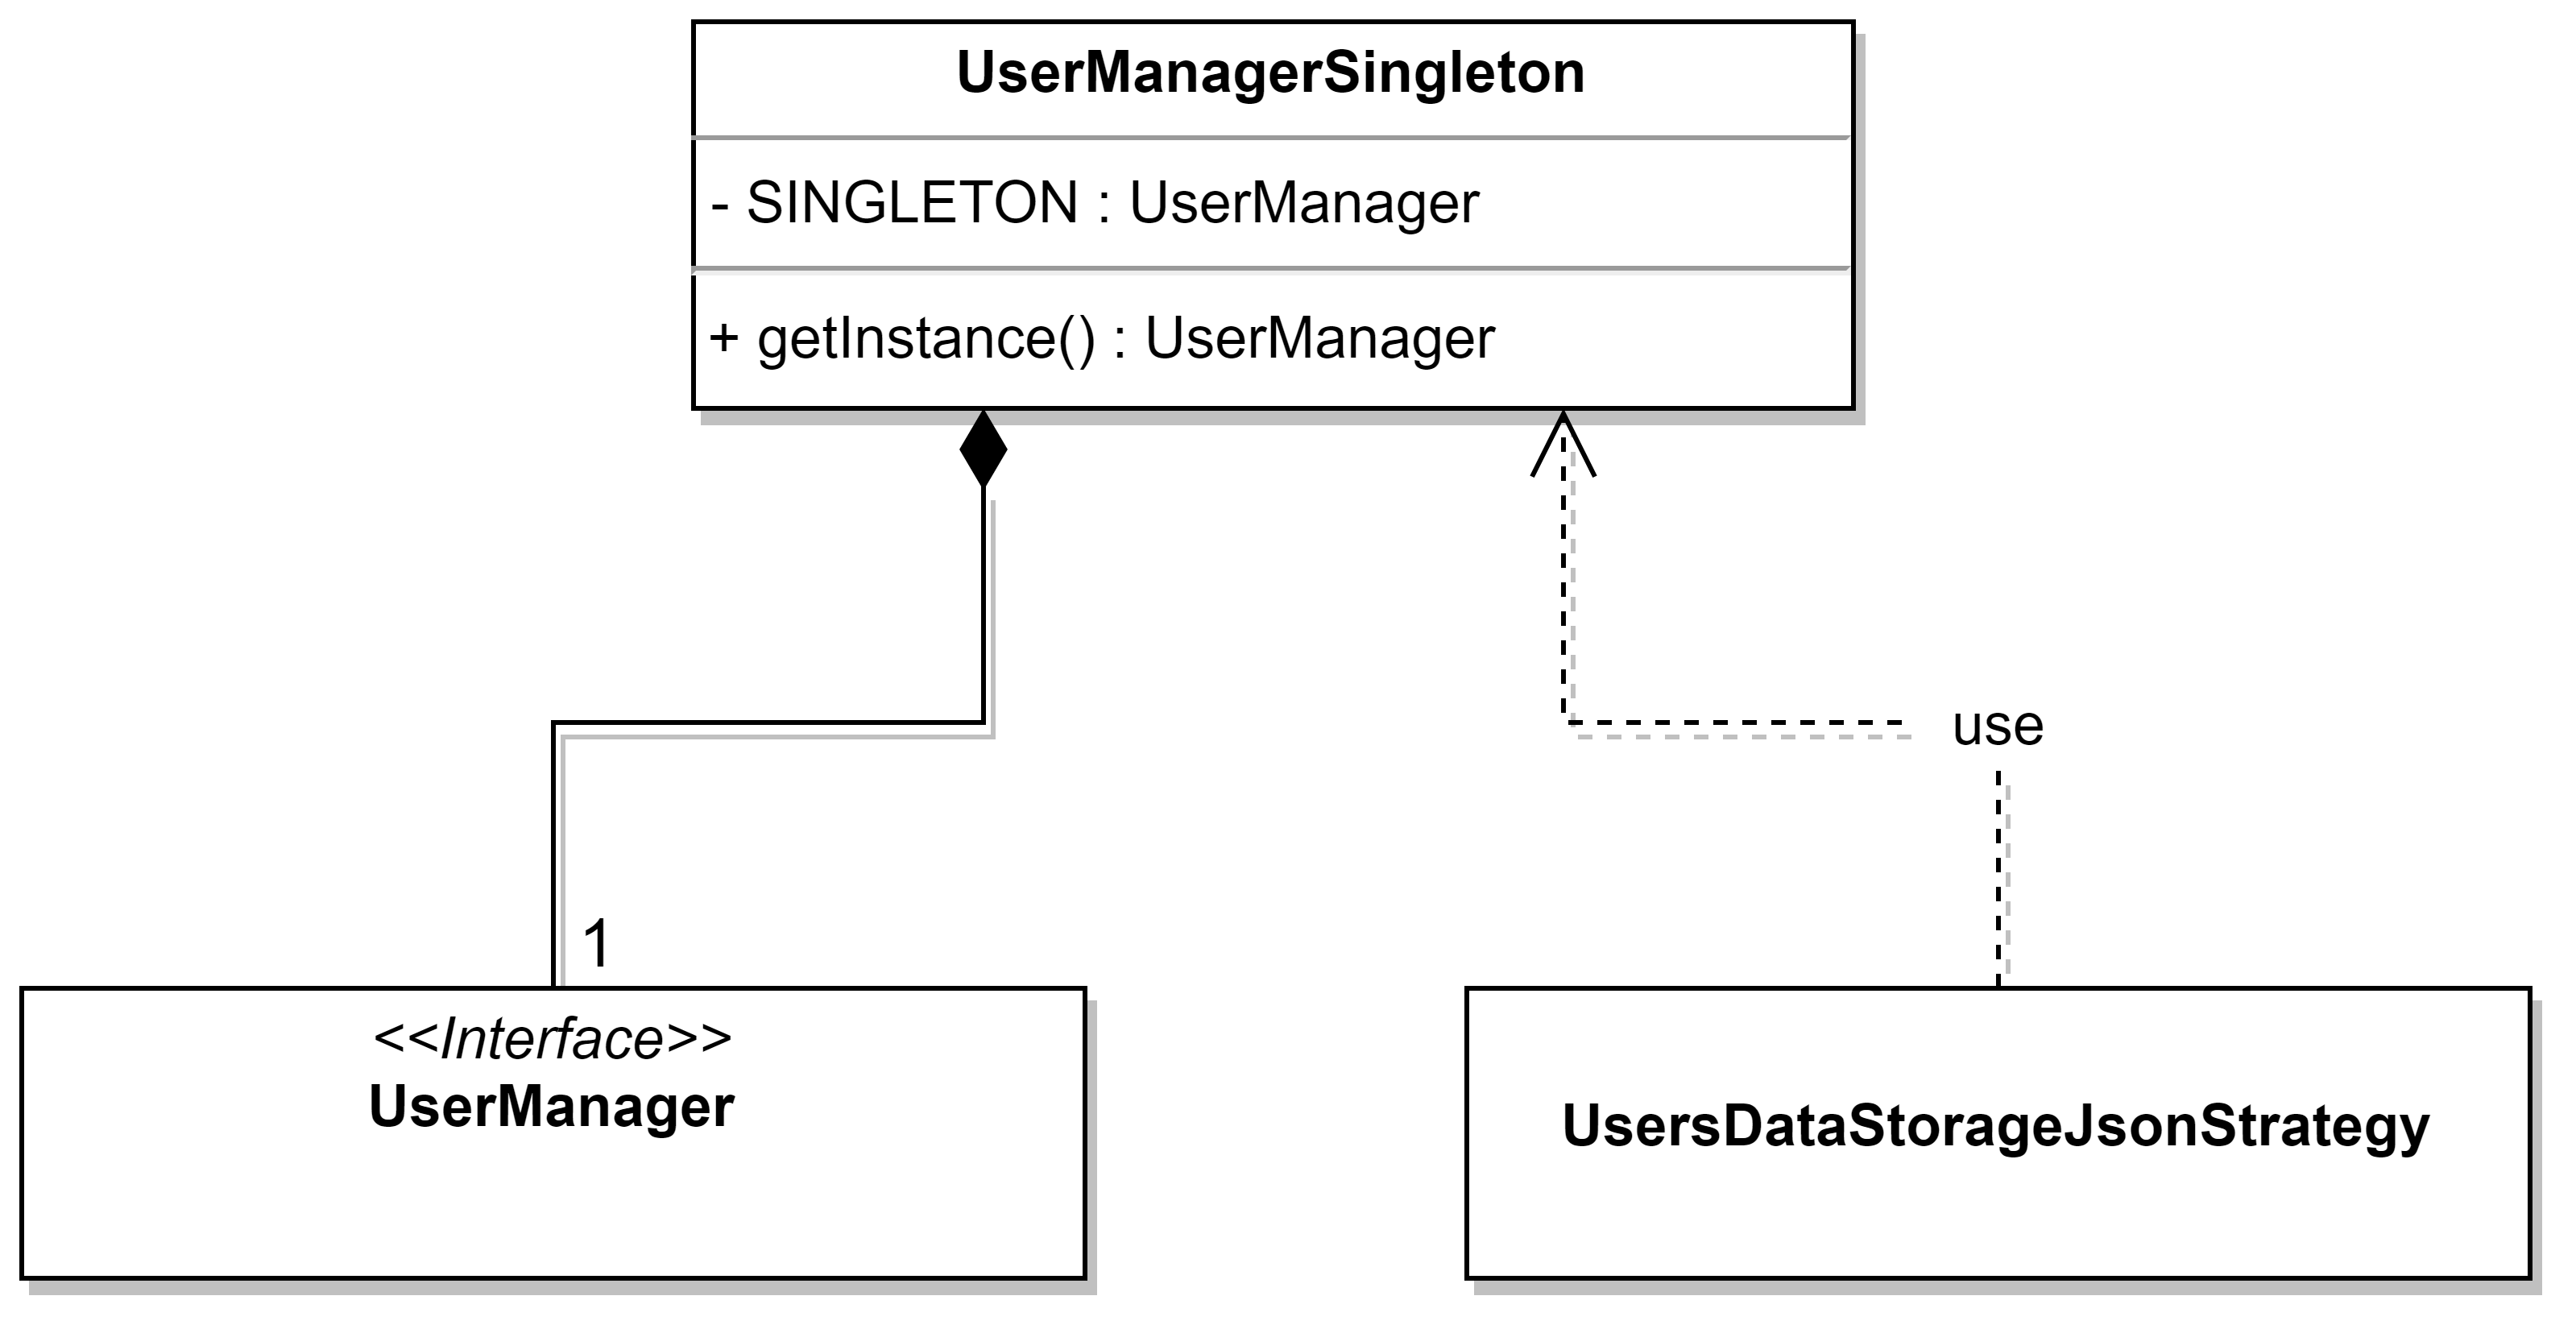
\includegraphics[width=\textwidth]{img/Manuel/shadow/Singleton.png}
    \end{center}
    \caption{Singleton utilizzato per un accesso unificato}
    \label{img:Singleton}
\end{figure}
%

\subsubsection*{Classifica}

Nel momento in cui ho dovuto iniziare a pensare alla classifica, sarebbe bastato prendere tutti gli utenti dell'applicazione, con annessi i loro punteggi, e stamparli ove necessario. In questo caso non avrei dovuto implementare nient'altro, sarebbe bastato lo \texttt{\nameref{UserManager}}. Questa soluzione avrebbe soddisfatto i requisiti minimi di ciò che avevamo deciso, ma non sarebbe stata efficiente, infatti ogni funzionalità aggiuntiva avrebbe comportato ulteriore codice.
\\
Fatta questa premessa infatti, ho pensato che fosse giusto l'utilizzo del pattern \textbf{Builder}, il quale mi avrebbe lasciato libertà di dividere la creazione della \texttt{Leaderboard}. Se in futuro aumentassero le responsabilità della classifica, non si andrebbe ad intaccare il codice già scritto.
Con i metodi \texttt{addUsers()}, \texttt{addFilter()} e \texttt{comparator()} è possibile manipolare i dati, creando classifiche parziali e non, mentre su \texttt{strategy()} ci torneremo in seguito.
\\
Sulla definizione dell'interfaccia \texttt{Leaderboard} ho notato non fosse corretto utilizzare una lista di \texttt{\nameref{User}}, proprio perché in questa situazione non sono necessarie tutte le informazioni interne dello stesso (e.g. password). Questo fatto mi ha portato ad utilizzare il pattern \textbf{Adapter}: la \texttt{LeaderboardUserAdapter} è l'interfaccia che cattura i dati dell'utente che realmente andranno in classifica. Infatti, questo pattern mi permette di aggiungere metodi specifici, ove necessari.
\\
Proprio sul fatto di aggiungere responsabilità, ho deciso di assegnare un punteggio all'utente da andare ad inserire nella classifica: questa modifica non va ad intaccare lo \texttt{\nameref{User}}, grazie alle scelte illustrate in precedenza.
\\
Per la gestione del punteggio ho pensato di utilizzare il pattern \textbf{Strategy}: questa scelta mi lascia la libertà di attribuire punteggi in base alle necessità.
\\
Ho deciso di passare la strategia al Builder, proprio per avere congruenza sui dati: questo mi permette infatti di avere la stessa valutazione di punteggio all'interno della medesima classifica.

% Leaderboard
\begin{figure}[ht]
    \begin{center}
        \centering
        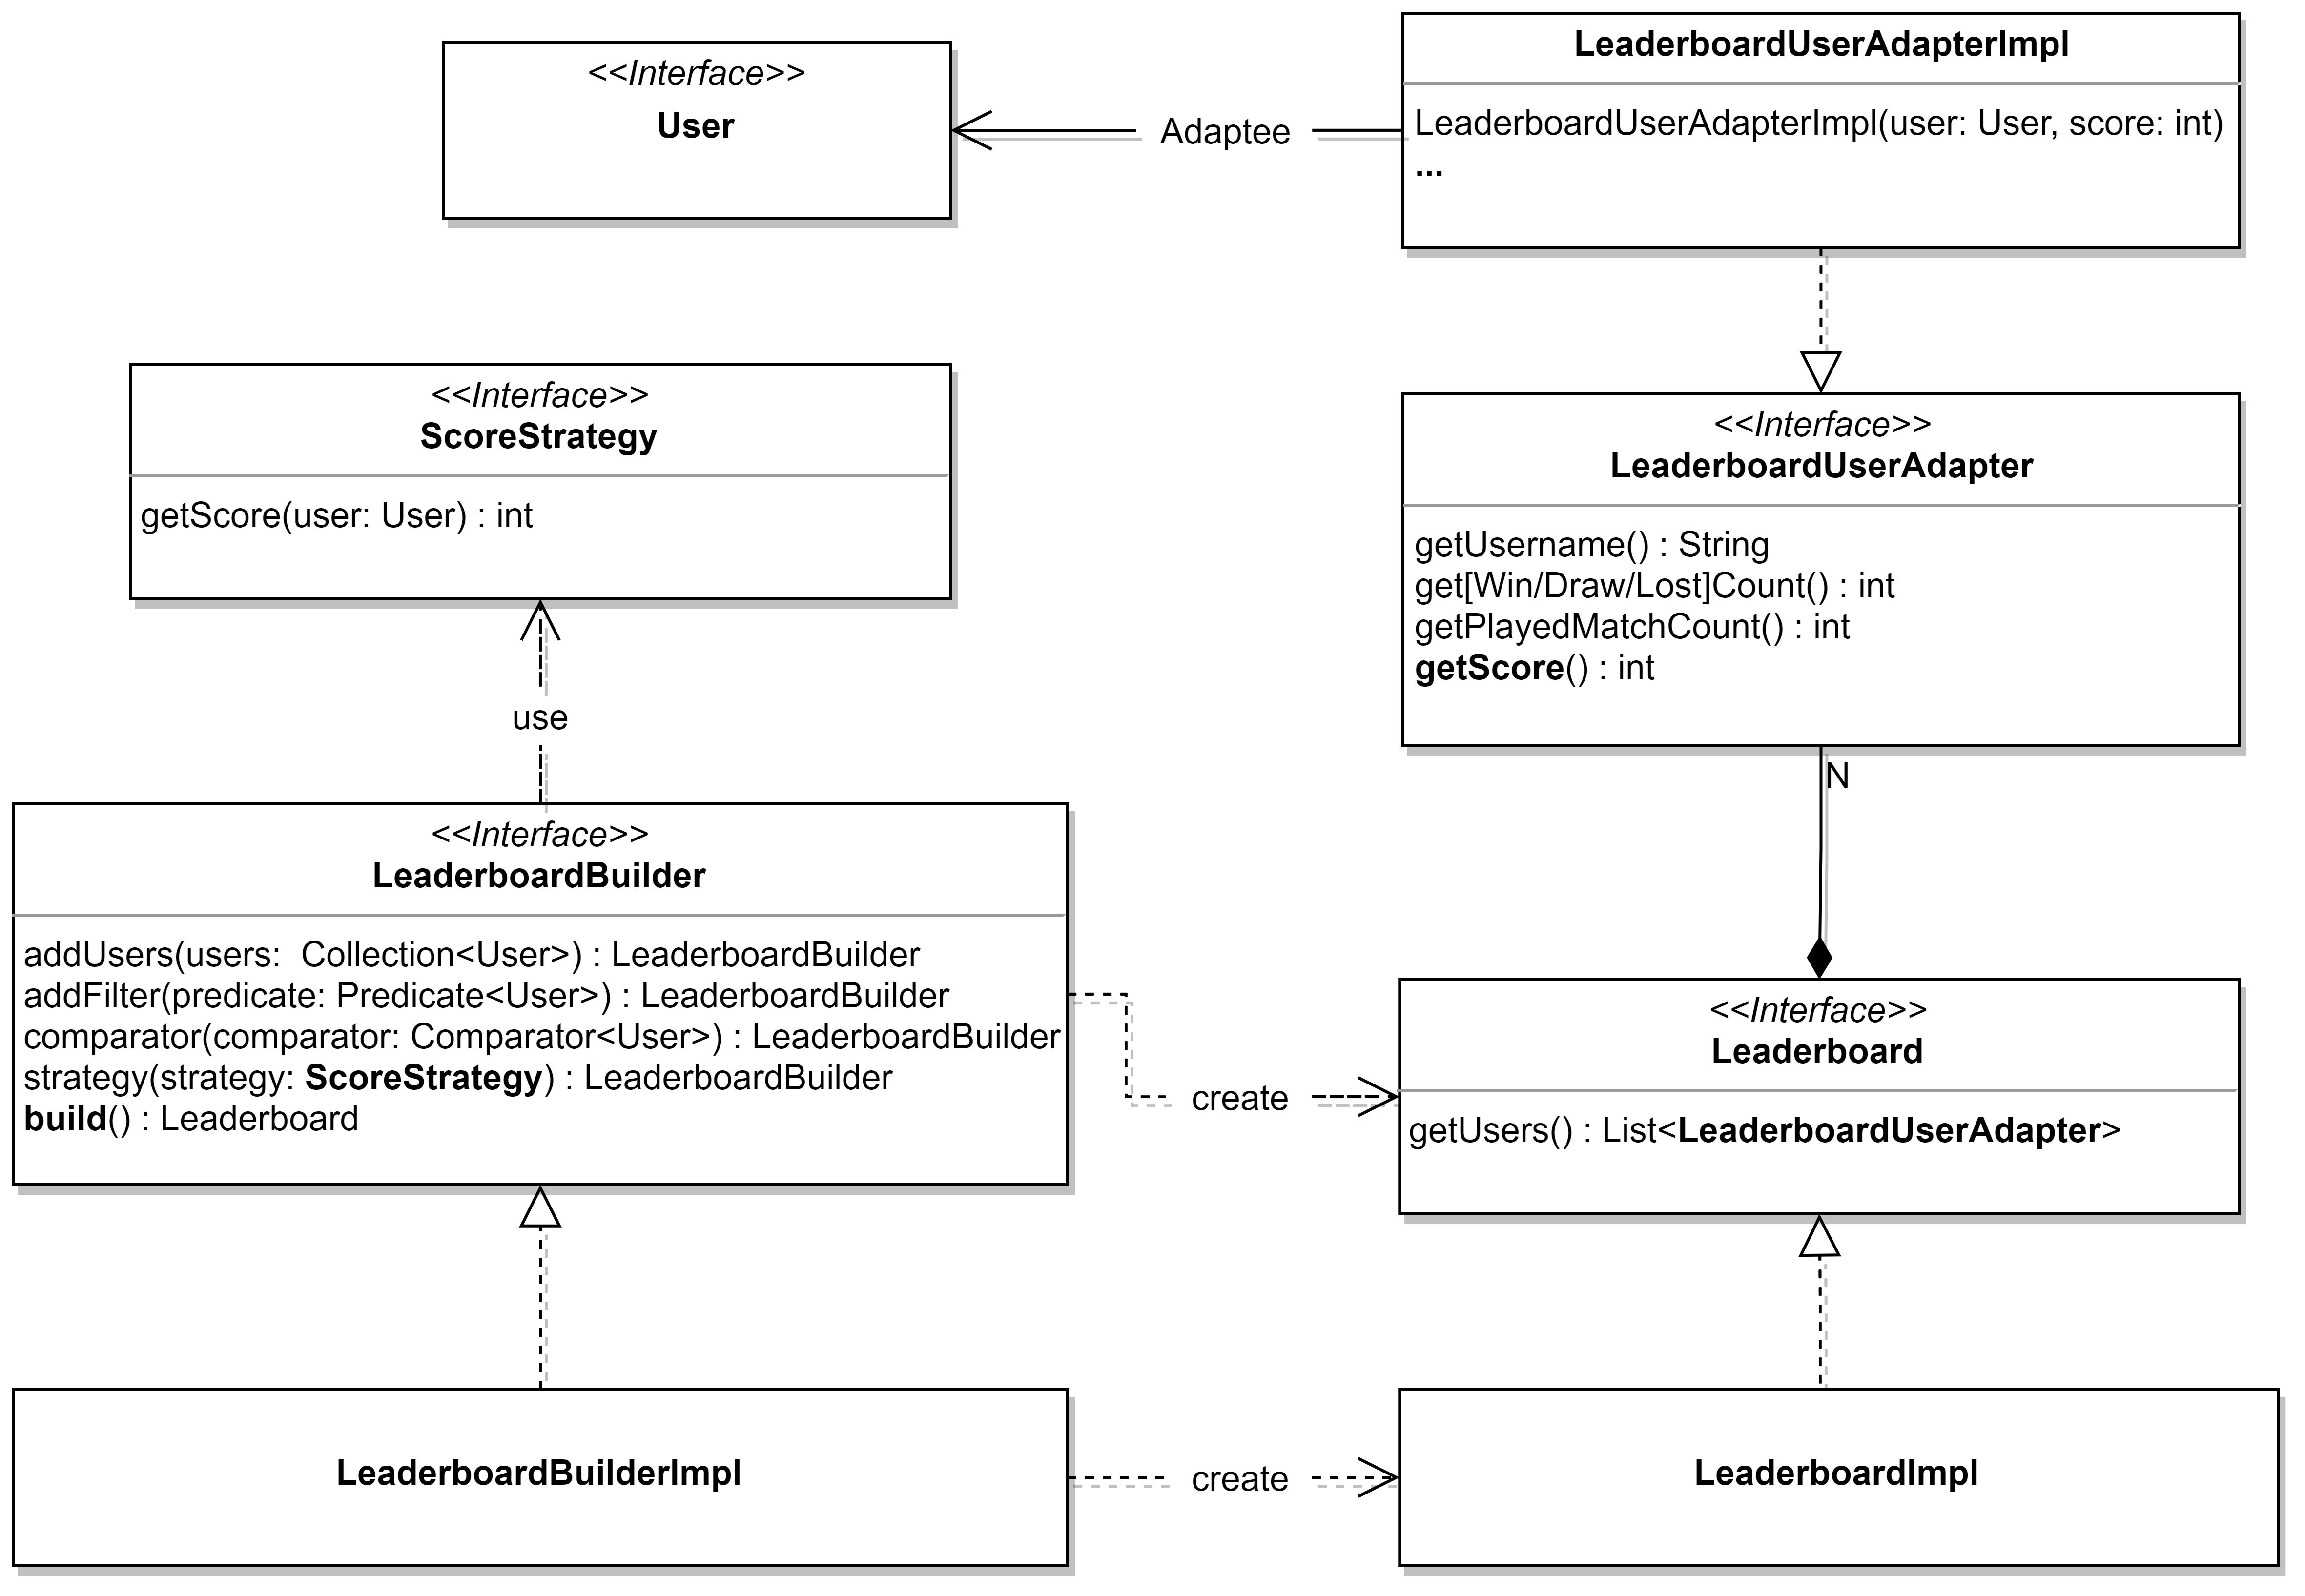
\includegraphics[width=\textwidth]{img/Manuel/shadow/Leaderboard.png}
    \end{center}
    \caption{Leaderboard: creazione e contenuto}
    \label{img:Leaderboard}
\end{figure}
%

\clearpage
\subsection{Mazzoli Alessandro}

\subsubsection{Player}
\label{Player}

Durante la fasi di analisi, si è deciso di dividere l'entità \texttt{\nameref{User}} dall'entità \texttt{Player}, che ricoprono due ruoli differenti. La prima, trattata in un altro paragrafo apposito, gestisce l'utente che accede all'applicazione, mentre la seconda si occuperà del giocatore effettivo durante la partita. Il \texttt{Player} avrà una referenza allo \texttt{User} a cui è legato.
\\
Nel gioco degli scacchi ogni player è identificato da un colore, che nel nostro caso è rappresentato dalla enum \texttt{PlayerColor}. Questo colore nella versione base degli scacchi può essere o bianco o nero, tuttavia avendola gestita come enumeration questo permette l'estensibilità ad un numero più elevato di colori in modo da gestire partite con un numero più elevato di giocatori (ad esempio potrebbe esistere una variante degli scacchi che si gioca in 4).
\\
Per la generazione dei pezzi è stato scelto il pattern \textbf{Factory}, infatti ogni player ha dentro di se una \texttt{PieceFactory}, che verrà usata per generare i propri pezzi, in modo da avere in essi una referenza al colore.
\paragraph{}

%
\begin{figure}[H]
    \begin{center}
        \centering
        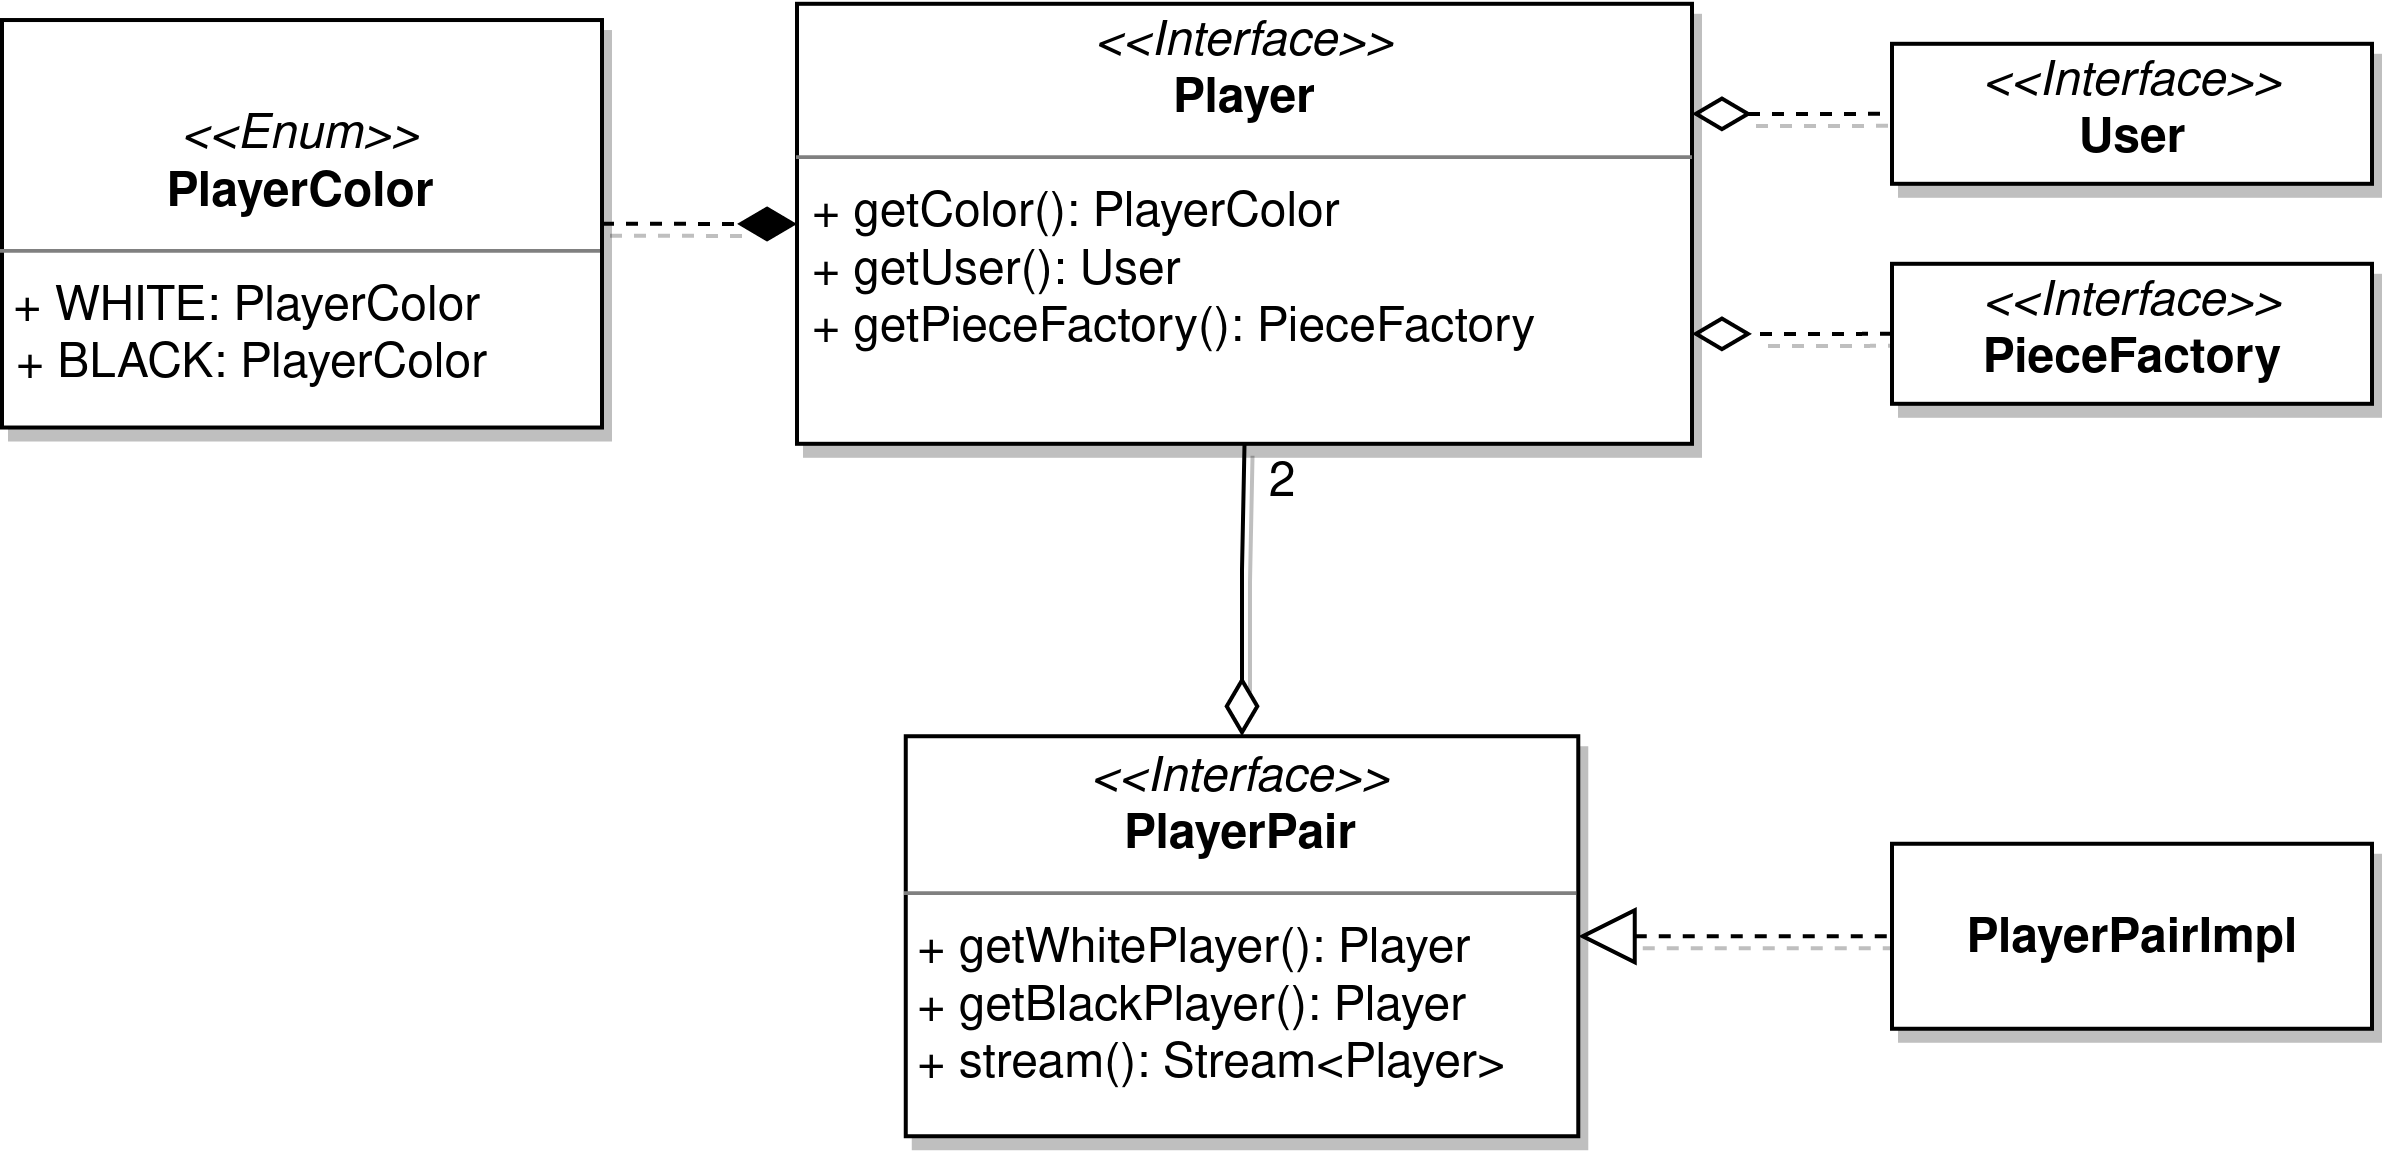
\includegraphics[width=\textwidth]{img/Alessandro/players.png}
    \end{center}
    \caption{Gestione dei Players}
    \label{img:players}
\end{figure}
%
\
\\
Dato che si è scelto di gestire solamente varianti che hanno due giocatori, si ha avuto la necessita di salvarsi sempre la coppia whitePlayer e blackPlayer in molte parti del motore scacchistico. Ho quindi deciso di creare una classe specifica per contenerli: la \texttt{PlayerPair}. Questa fornisce l'accesso al whitePlayer ed al blackPlayer tramite getter specifici.
\\
Inizialmente infatti si era optato di utilizzare una Pair generica, tuttavia si doveva usare una convenzione di accesso, ovvero: facendo getX() veniva restituito il whitePlayer e con getY() veniva restituito il blackPlayer.
\\
Questo tuttavia creava molta confusione ed il codice risultava opaco, mentre con l'utilizzo della classe \texttt{PlayerPair} è stata rimossa questa problematica.

\subsubsection{Game}
\label{Game}

L'applicazione, come già premesso, deve supportare più varianti scacchistiche, non solo la modalità classica.\\
Per permetterne un' efficace funzionamento abbiamo dovuto analizzare dal punto di vista teorico ciò che caratterizza e differenzia le varie componenti di una modalità di gioco scacchistica, giungendo ad un breakdown in componenti essenziali della stessa.
\\
Questa modalità di gioco è stata identificata quindi dall'interfaccia \texttt{Game}, tenendo conto che esso è composto da 3 macro-componenti:
\begin{itemize}
	\item un \texttt{GameType}, ovvero il tipo di gioco a cui stiamo giocando, definito tramite una enumeration, che avrà dentro di sè informazioni quali il nome e una breve descrizione.
	\item un \texttt{MovementManager}, che si occupa dell'effettuare i movimenti dei pezzi controllando la loro fattibilità.
	\item un \texttt{GameController}, il cui scopo è quello di conoscere lo stato della partita, rilevare scacchi, stalli e controllare se la partita è giunta ad una conclusione o meno.
\end{itemize}
Possiamo vedere quindi il Game come un wrapper racchiudente le componenti sopra citate.
\
%
\begin{figure}[H]
    \begin{center}
        \centering
        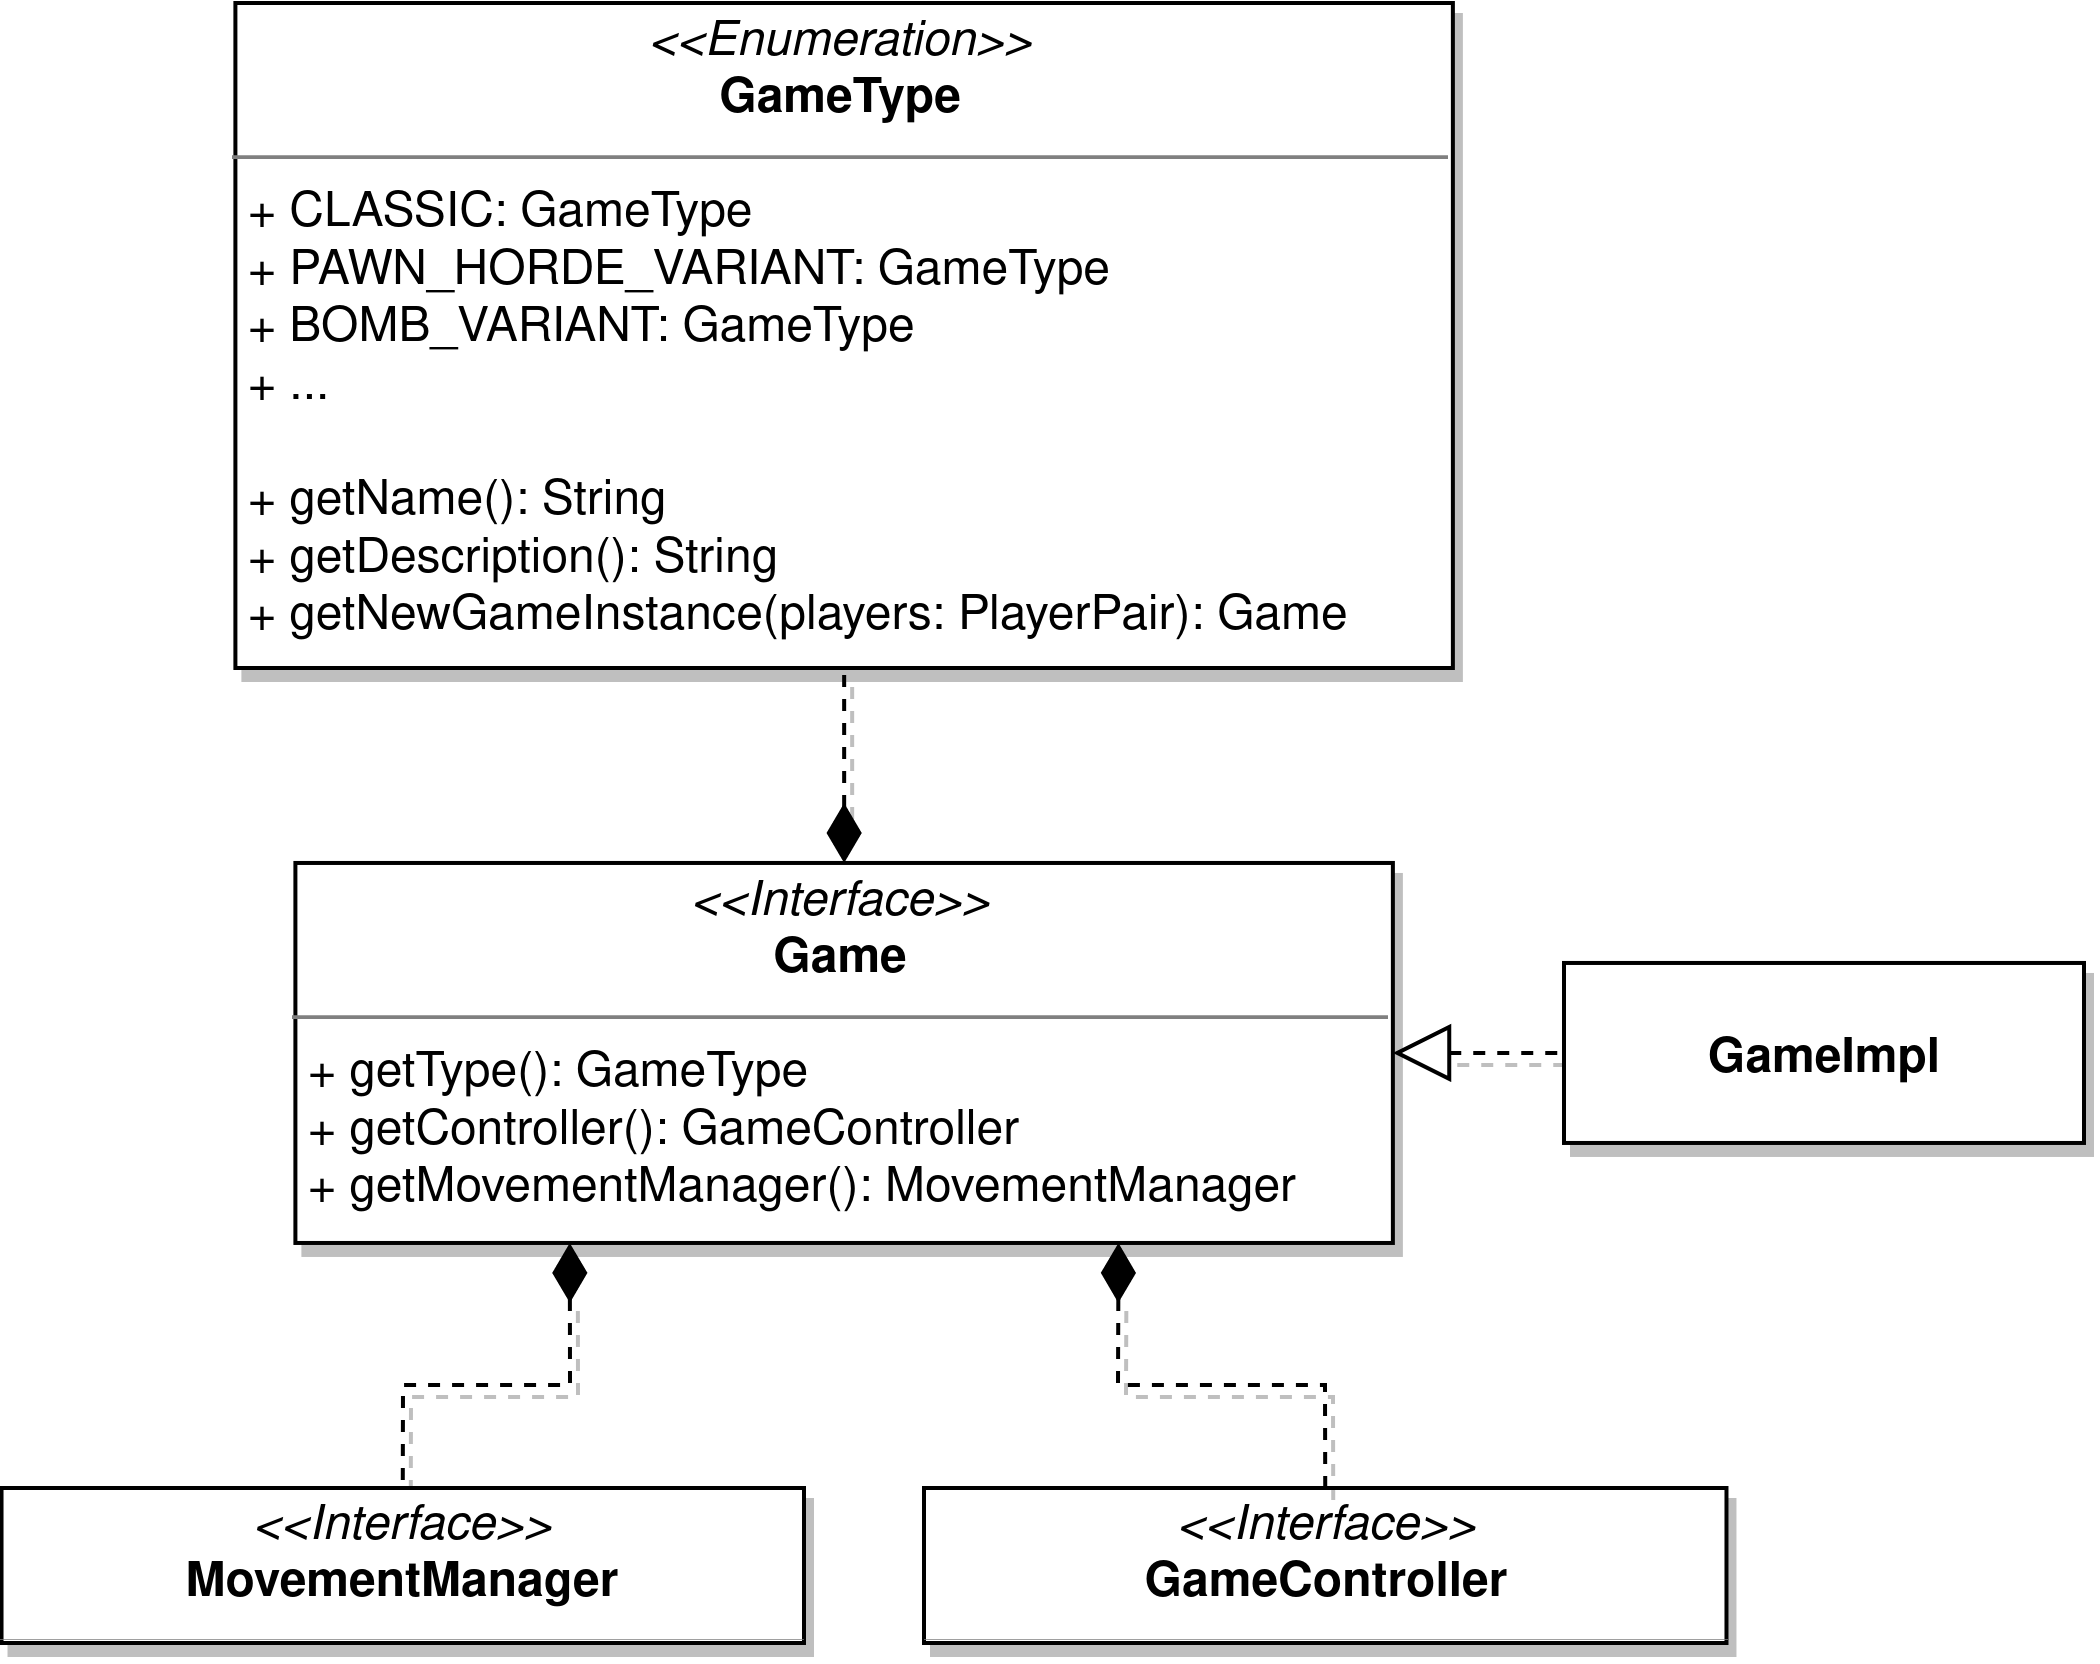
\includegraphics[width=\textwidth]{img/Alessandro/game_management.png}
    \end{center}
    \caption{Gestione della struttura di una modalità di gioco degli scacchi con un alto livello di estensibilità}
    \label{img:game_management}
\end{figure}
%
\
\\
Per la creazione di un' istanza di Game, si è deciso di utilizzare il pattern \textbf{Factory} tramite l'interfaccia \texttt{GameFactory}.
A questa è stato delegato il compito della creazione di istanze delle varie tipologie di \texttt{Game}.
\\
Il suo compito è di generare le componenti adatte alla modalità di gioco richiesta, andando quindi a creare per ogni tipo di \texttt{Game} un istanza di ogni sua componente interna citata precedentemente.
\\
Si è scelto inoltre di utilizzare anche il pattern \textbf{Builder} nel \texttt{GameBuilder}. Nonostante i parametri del Game non siano molti, ho scelto di farne comunque uso perché ritengo se ne guadagni dal punto di vista della leggibilità del codice quando si tratta di creare un'istanza di un determinato oggetto.
%
\begin{figure}[H]
    \begin{center}
        \centering
        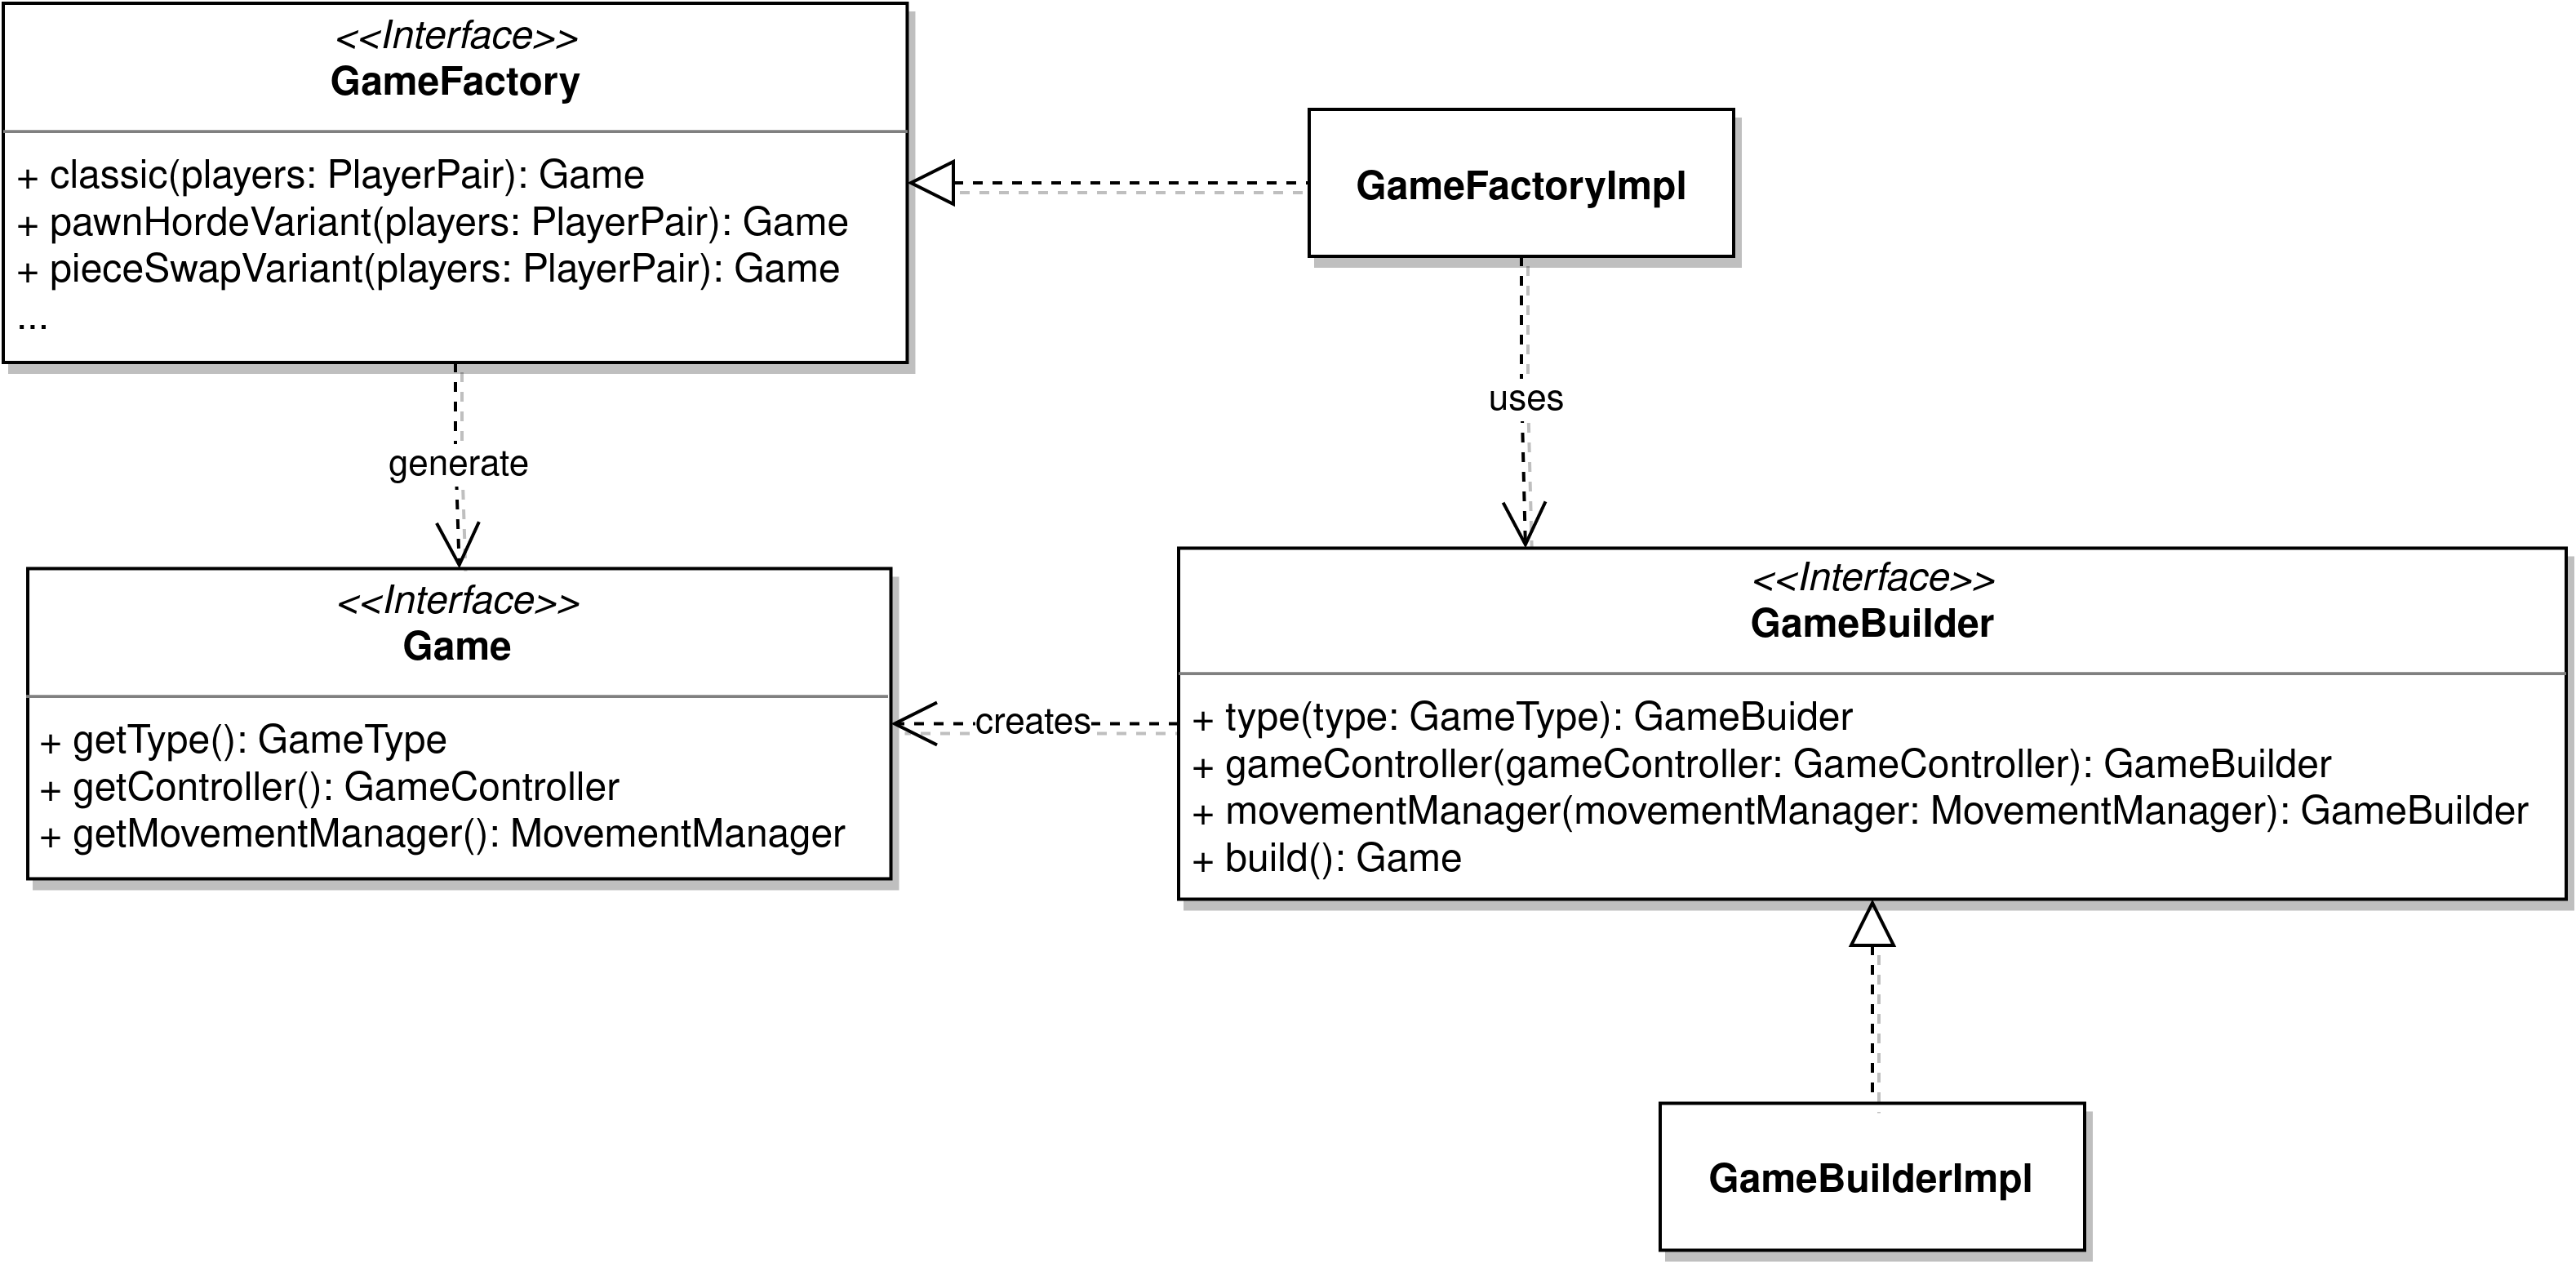
\includegraphics[width=\textwidth]{img/Alessandro/game_creation.png}
    \end{center}
    \caption{Creazione di un Game tramite pattern Factory e Builder}
    \label{img:game_creation}
\end{figure}
%
\paragraph{}
\
\\
Si può notare la corrispondenza 1:1 tra una entry di \texttt{GameType} e di \texttt{Game}, infatti quello che ne risulta è che per ogni entry della Enum vi è un metodo nella \texttt{GameFactory} per creare un oggetto di quel tipo.
\\
Sarebbe stato possibile incapsulare la creazione di questo oggetto totalmente all' interno dell'Enum \texttt{GameType}, tuttavia avrebbe portato ad un elevato numero di responsabilità delegate a quest'ultima e ne avrebbe aumentato notevolmente le dimensioni.
\\
Quello a cui si è giunti è quindi un compromesso tra le due cose, poiché è molto comodo ottenere un' istanza di un Game dato il \texttt{GameType}, abbiamo aggiunto un metodo \texttt{getNewGameInstance(...)} all'interno dell'Enum che permette di ritornare una nuova istanza di un \texttt{Game} relativo a quel \texttt{GameType}. Questo metodo utilizza internamente una \texttt{GameFactory}, ed ogni entry di \texttt{GameType} deve specificare una strategia di creazione di quel determinato Game avendo come input la \texttt{GameFactory} e i players.
\\
Questo è stato ottenuto utilizzando il pattern \textbf{Strategy} attraverso l'interfaccia funzionale \texttt{GameGenerationStrategy} il cui unico metodo permette di creare un' istanza di Game prendendo come parametri la \texttt{GameFactory} interna all'enum ed i players.
%
\begin{figure}[H]
    \begin{center}
        \centering
        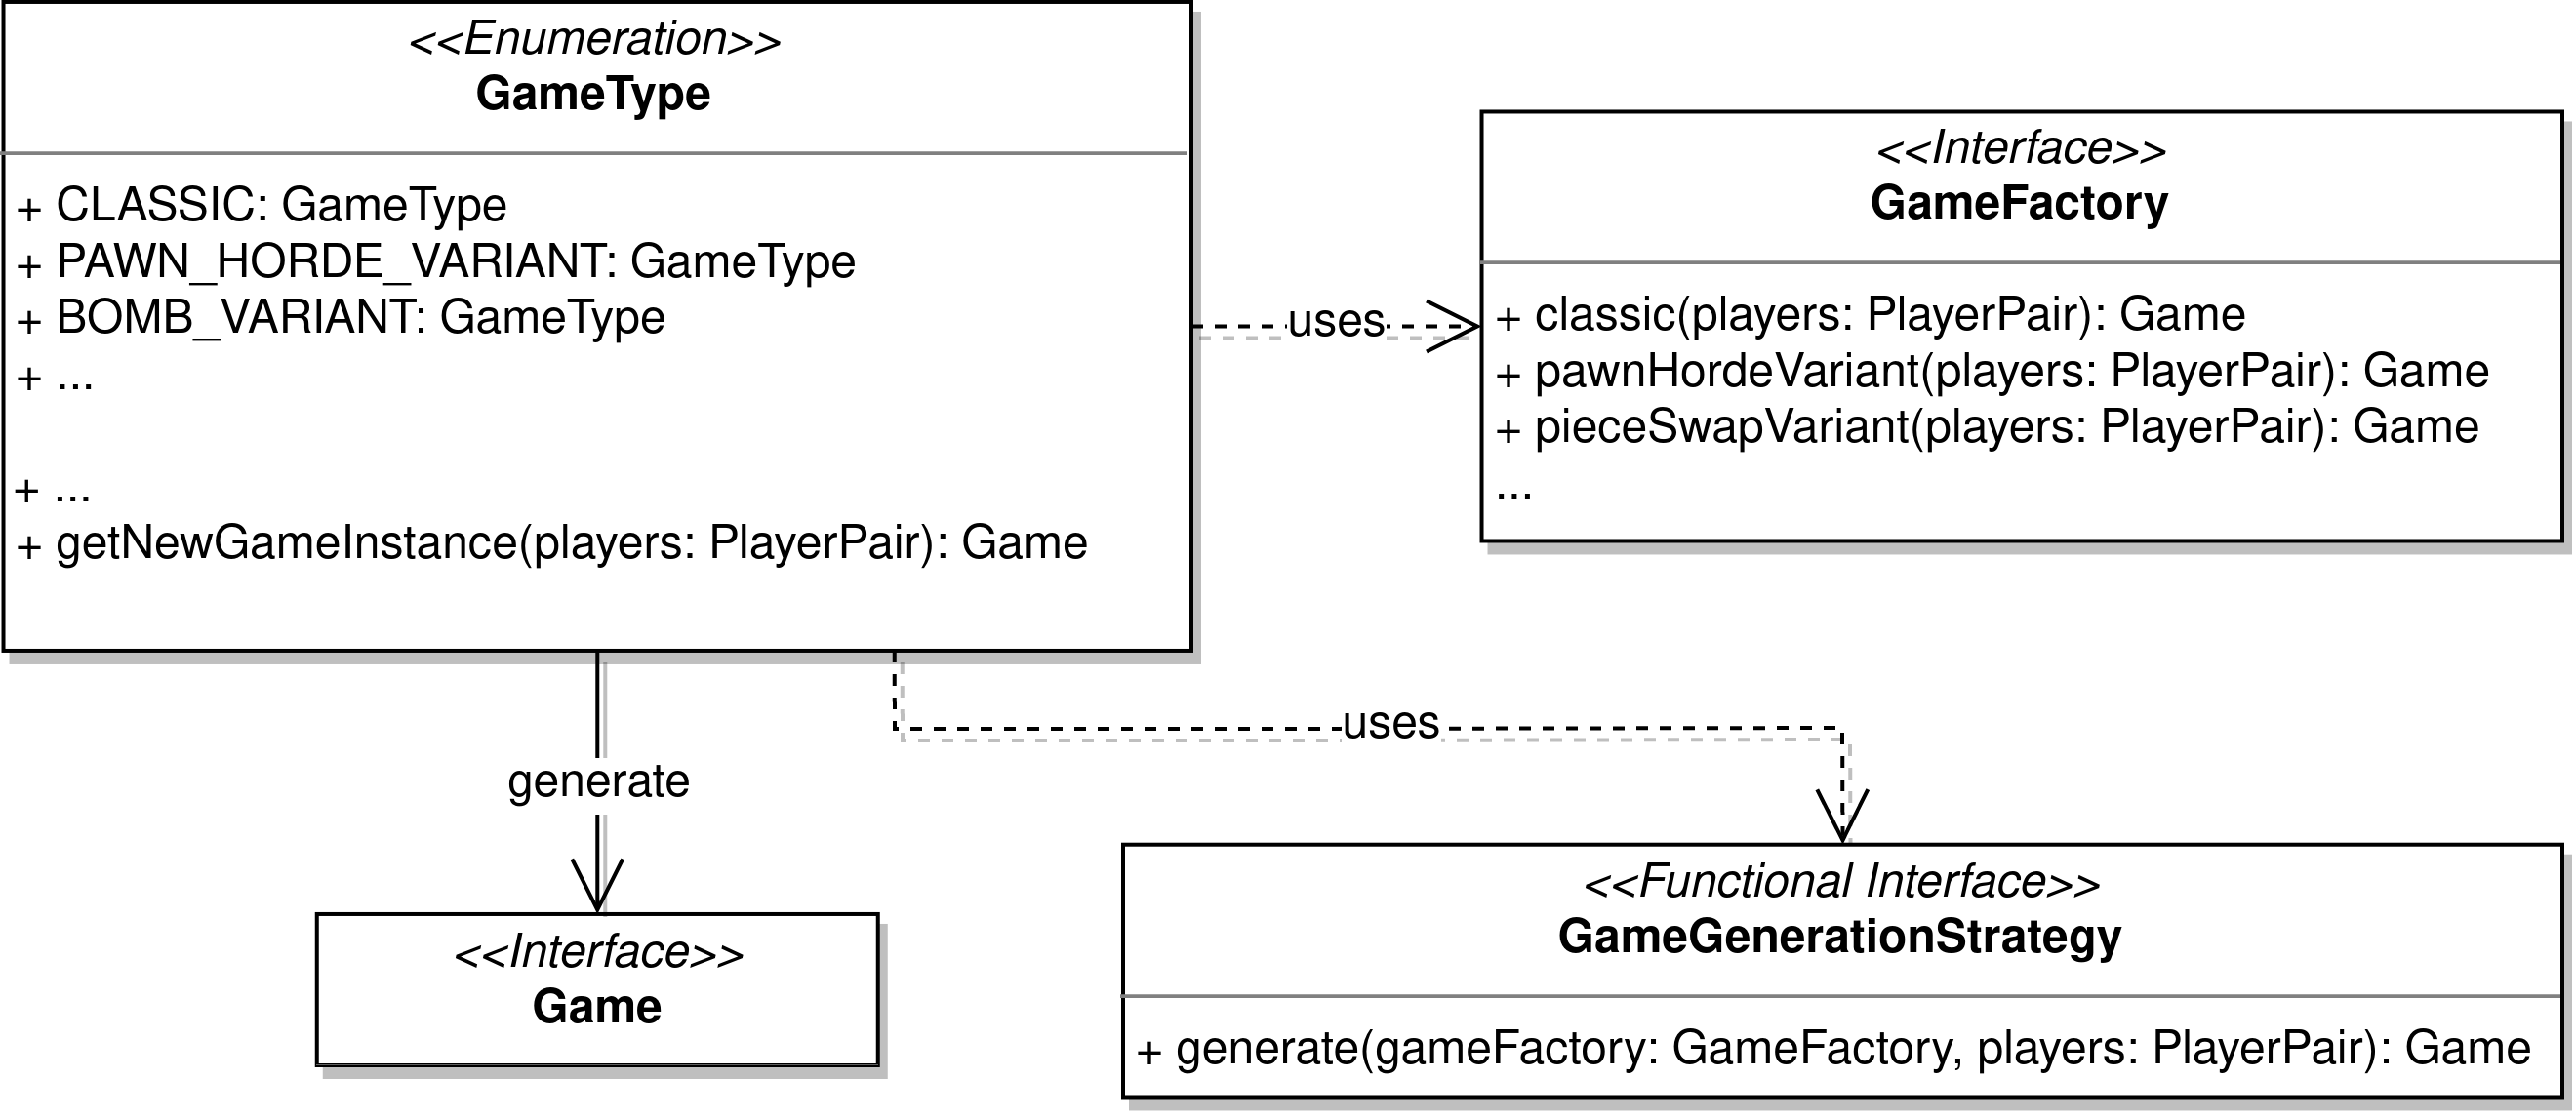
\includegraphics[width=\textwidth]{img/Alessandro/game_generation.png}
    \end{center}
    \caption{Generazione del Game in maniera agevole tramite pattern Strategy}
    \label{img:game_generation}
\end{figure}
%

\subsubsection{Match}
Come già fatto con la gestione di \texttt{Player} e \texttt{User}, anche in questo caso ho deciso di differenziare l'entità \texttt{Game} dall'entità \texttt{Match}.
\\
Il \texttt{Game}, come già detto precedentemente, è l'istanza del gioco attuale, comprensivo del suo progressivo stato durante la partita e delle sue regole, mentre il Match si può considerare un "wrapper" che gli aggiunge funzionalità.
\\
Una partita vera e propria, infatti, non è rappresentata della sola entità Game ma necessita della presenza di altri componenti, tra i quali un Timer e la \texttt{History} della partita(la sequenza di mosse/stati eseguite).
\\
Affidare tutte queste responsabilità all'entità \texttt{Game} avrebbe violato fortemente SRP e quindi si è optato per l'utilizzo dell'entità \texttt{Match}, che internamente ha l'istanza del \texttt{Game} ed inoltre tiene conto di tutte le altre componenti che compongono una vera partita di scacchi.
\\
Il controller della partita comunicherà quindi con questa entità, in essa troviamo infatti i metodi principali di gestione della partita, quali il metodo \texttt{move(...)} che permette di effettuare una mossa, il metodo \texttt{getPiecePossibleMoves(...)} che serve a restituire tutte le posizioni in cui può andare un determinato pezzo.
\\
Anche in questo caso il \texttt{MatchStatus} è stato considerato diverso dal \texttt{GameStatus}, in modo che gestisca semplicemente se la partita è attiva oppure terminata. In questo modo solamente una volta che l'utente sa che la partita è finita potrà andare a controllare come questa si è conclusa tramite il metodo \texttt{getEndType(...)}, che utilizza l' Enum che caratterizza tutti i modi in cui può finire una partita.
\\
Come si può notare, non abbiamo le stesse modalità di fine gioco del Game, infatti in questo caso oltre a \texttt{CHECKMATE} e \texttt{DRAW} vediamo comparire \texttt{RESIGN} e \texttt{TIMEOUT}, che come già detto sono feature esclusive del \texttt{Match} e sconosciute al \texttt{Game}.
%
\begin{figure}[H]
    \begin{center}
        \centering
        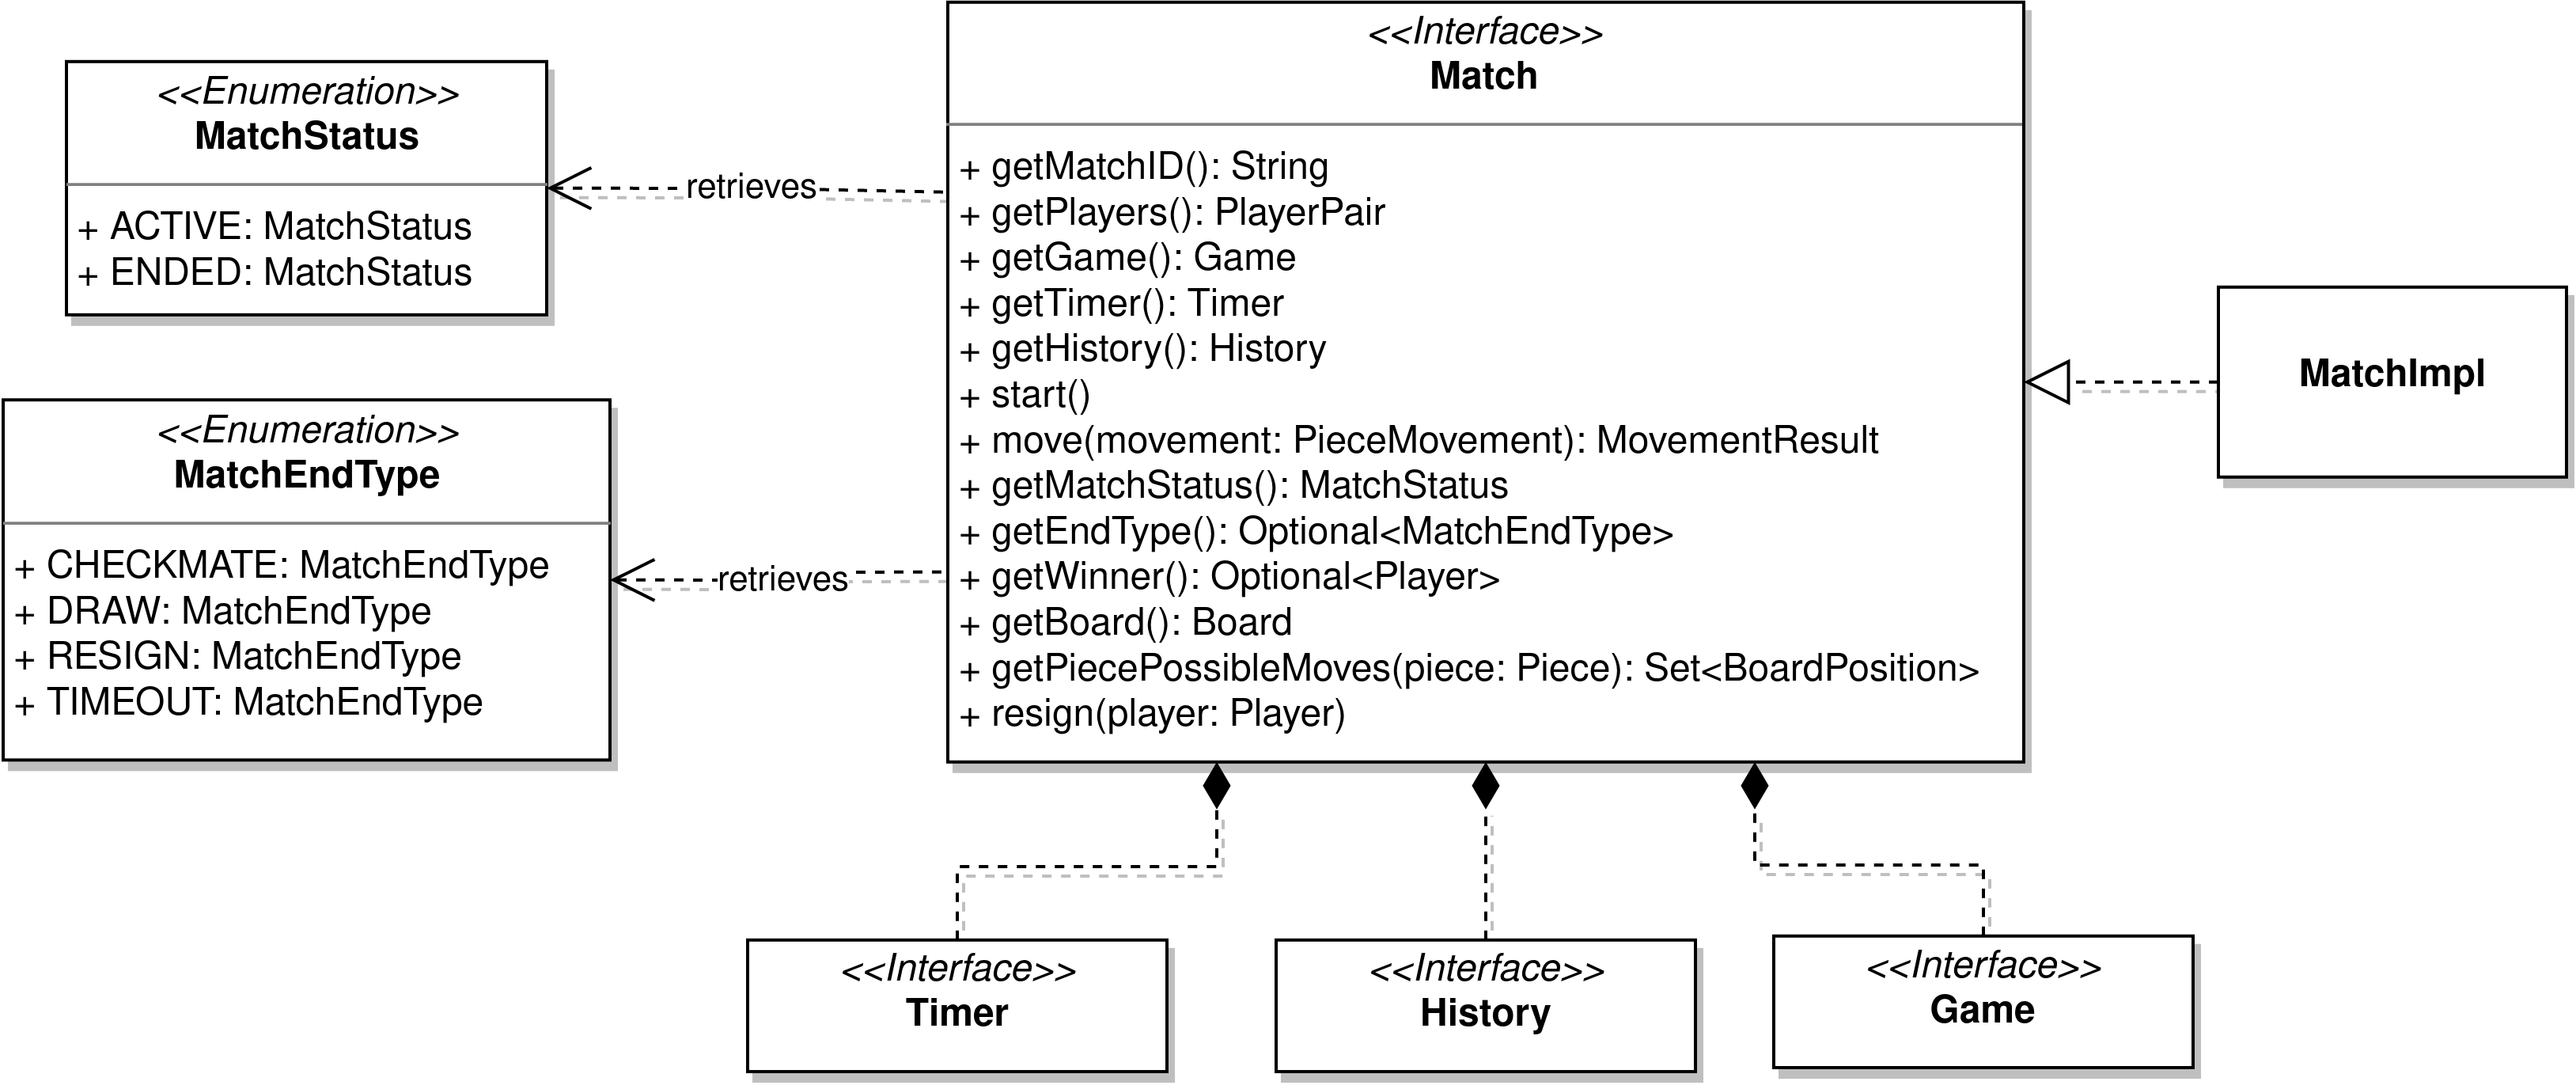
\includegraphics[width=\textwidth]{img/Alessandro/match.png}
    \end{center}
    \caption{Struttura di un Match comprensivo delle sue componenti e stati}
    \label{img:match}
\end{figure}

\subsubsection{Online Multiplayer}
Feature a cui ho molto tenuto sin dall'inizio dello sviluppo è stata la possibilità di giocare da due client diversi tramite internet, poiché questo permette di godersi molto di più il gioco non dando la necessità di essere in due persone davanti allo stesso computer per poter fare una partita.
\\
L'idea fin da subito era di utilizzare un mio server e crearci sopra un applicativo per la gestione della partita, tuttavia questo richiedeva di creare un database apposta per salvarsi le partite, gli utenti e soprattutto di trovare il modo di gestire in maniera efficiente la sincronizzazione tra i due client.
\\
Nonostante fosse tutto più che fattibile questo lavoro avrebbe portato via un quantitativo enorme di ore, ma il vero problema sarebbe stato che nel caso di utilizzo di questa modalità si sarebbe andato a perdere l'utilizzo del motore scacchistico da noi scritto, poiché il gestore della partita sarebbe stato il server (era quindi inoltre necessario reimplementare un altro motore).
\paragraph{}
\
\\
Non volendo rinunciare a questa feature ho deciso di creare una versione molto basilare di comunicazione via rete sfruttando il protocollo \texttt{MQTT} appoggiandomi al broker Mosquitto.
\\
Quello che fa quindi la modalità online è un handling della mossa utente e prima di inviarla al proprio motore la pubblica serializzata anche su un topic specifico tramite MQTT che comprende un base url 'jhaturanga/games/' concatenato al matchId.
In questo modo l'altro client che è sottoscritto a quel topic riceverà la mossa, la deserializzerà e la invierà al proprio motore interno facendola sembrare una mossa fatta dall'utente, triggherando successivamente una callBack che avviserà che è stata fatta una mossa.
\\
Quello che abbiamo è quindi che il \texttt{NetworkMatchManager} è colui che si occupa della creazione/join del match e dell'invio delle mosse all'altro client.
Tuttavia per non dargli troppe responsabilità la gestione dell'invio dei dati e della connessione/disconnessione dal broker è stata affidata all'entità \texttt{MqttNetworkInstance} il quale contratto è quello di permettere i metodi basilari di comunicazione tramite \texttt{MQTT} quali:
\begin{itemize}
    \item Connessione/Disconnesione
    \item Sottoscrizione ad un topic
    \item Invio di un determinato comando
\end{itemize}
La classe poi usata come implementazione di questo contratto è stata appunto la \texttt{MosquittoMqttNetworkInstance} che si serve del broker Mosquitto per la comunicazione.
\paragraph{}
\
\\
Per l'invio e la coordinazione dei messaggi è stato inoltre necessario trovare un modo per capire che cosa si stesse inviando/ricevendo e quindi si è sviluppata un entità che funzioni da DTO(Data Transfer Object) mediante l'utilizzo della classe \texttt{NetworkMessage}, che mi permette di incapsulare i dati da inviare memorizzando anche l'id di chi lo ha inviato.
\\
Quest'ultimo è servito poiché entrambi i client sono sia sottoscritti al topic e contemporaneamente ci pubblicano e quindi chi invia un messaggio lo riceve anche.
Avendo quindi a disposizione l'id di colui che invia posso filtrare i pacchetti in arrivo in modo da avere solo messaggi dell'altro client.
\begin{figure}[H]
    \begin{center}
        \centering
        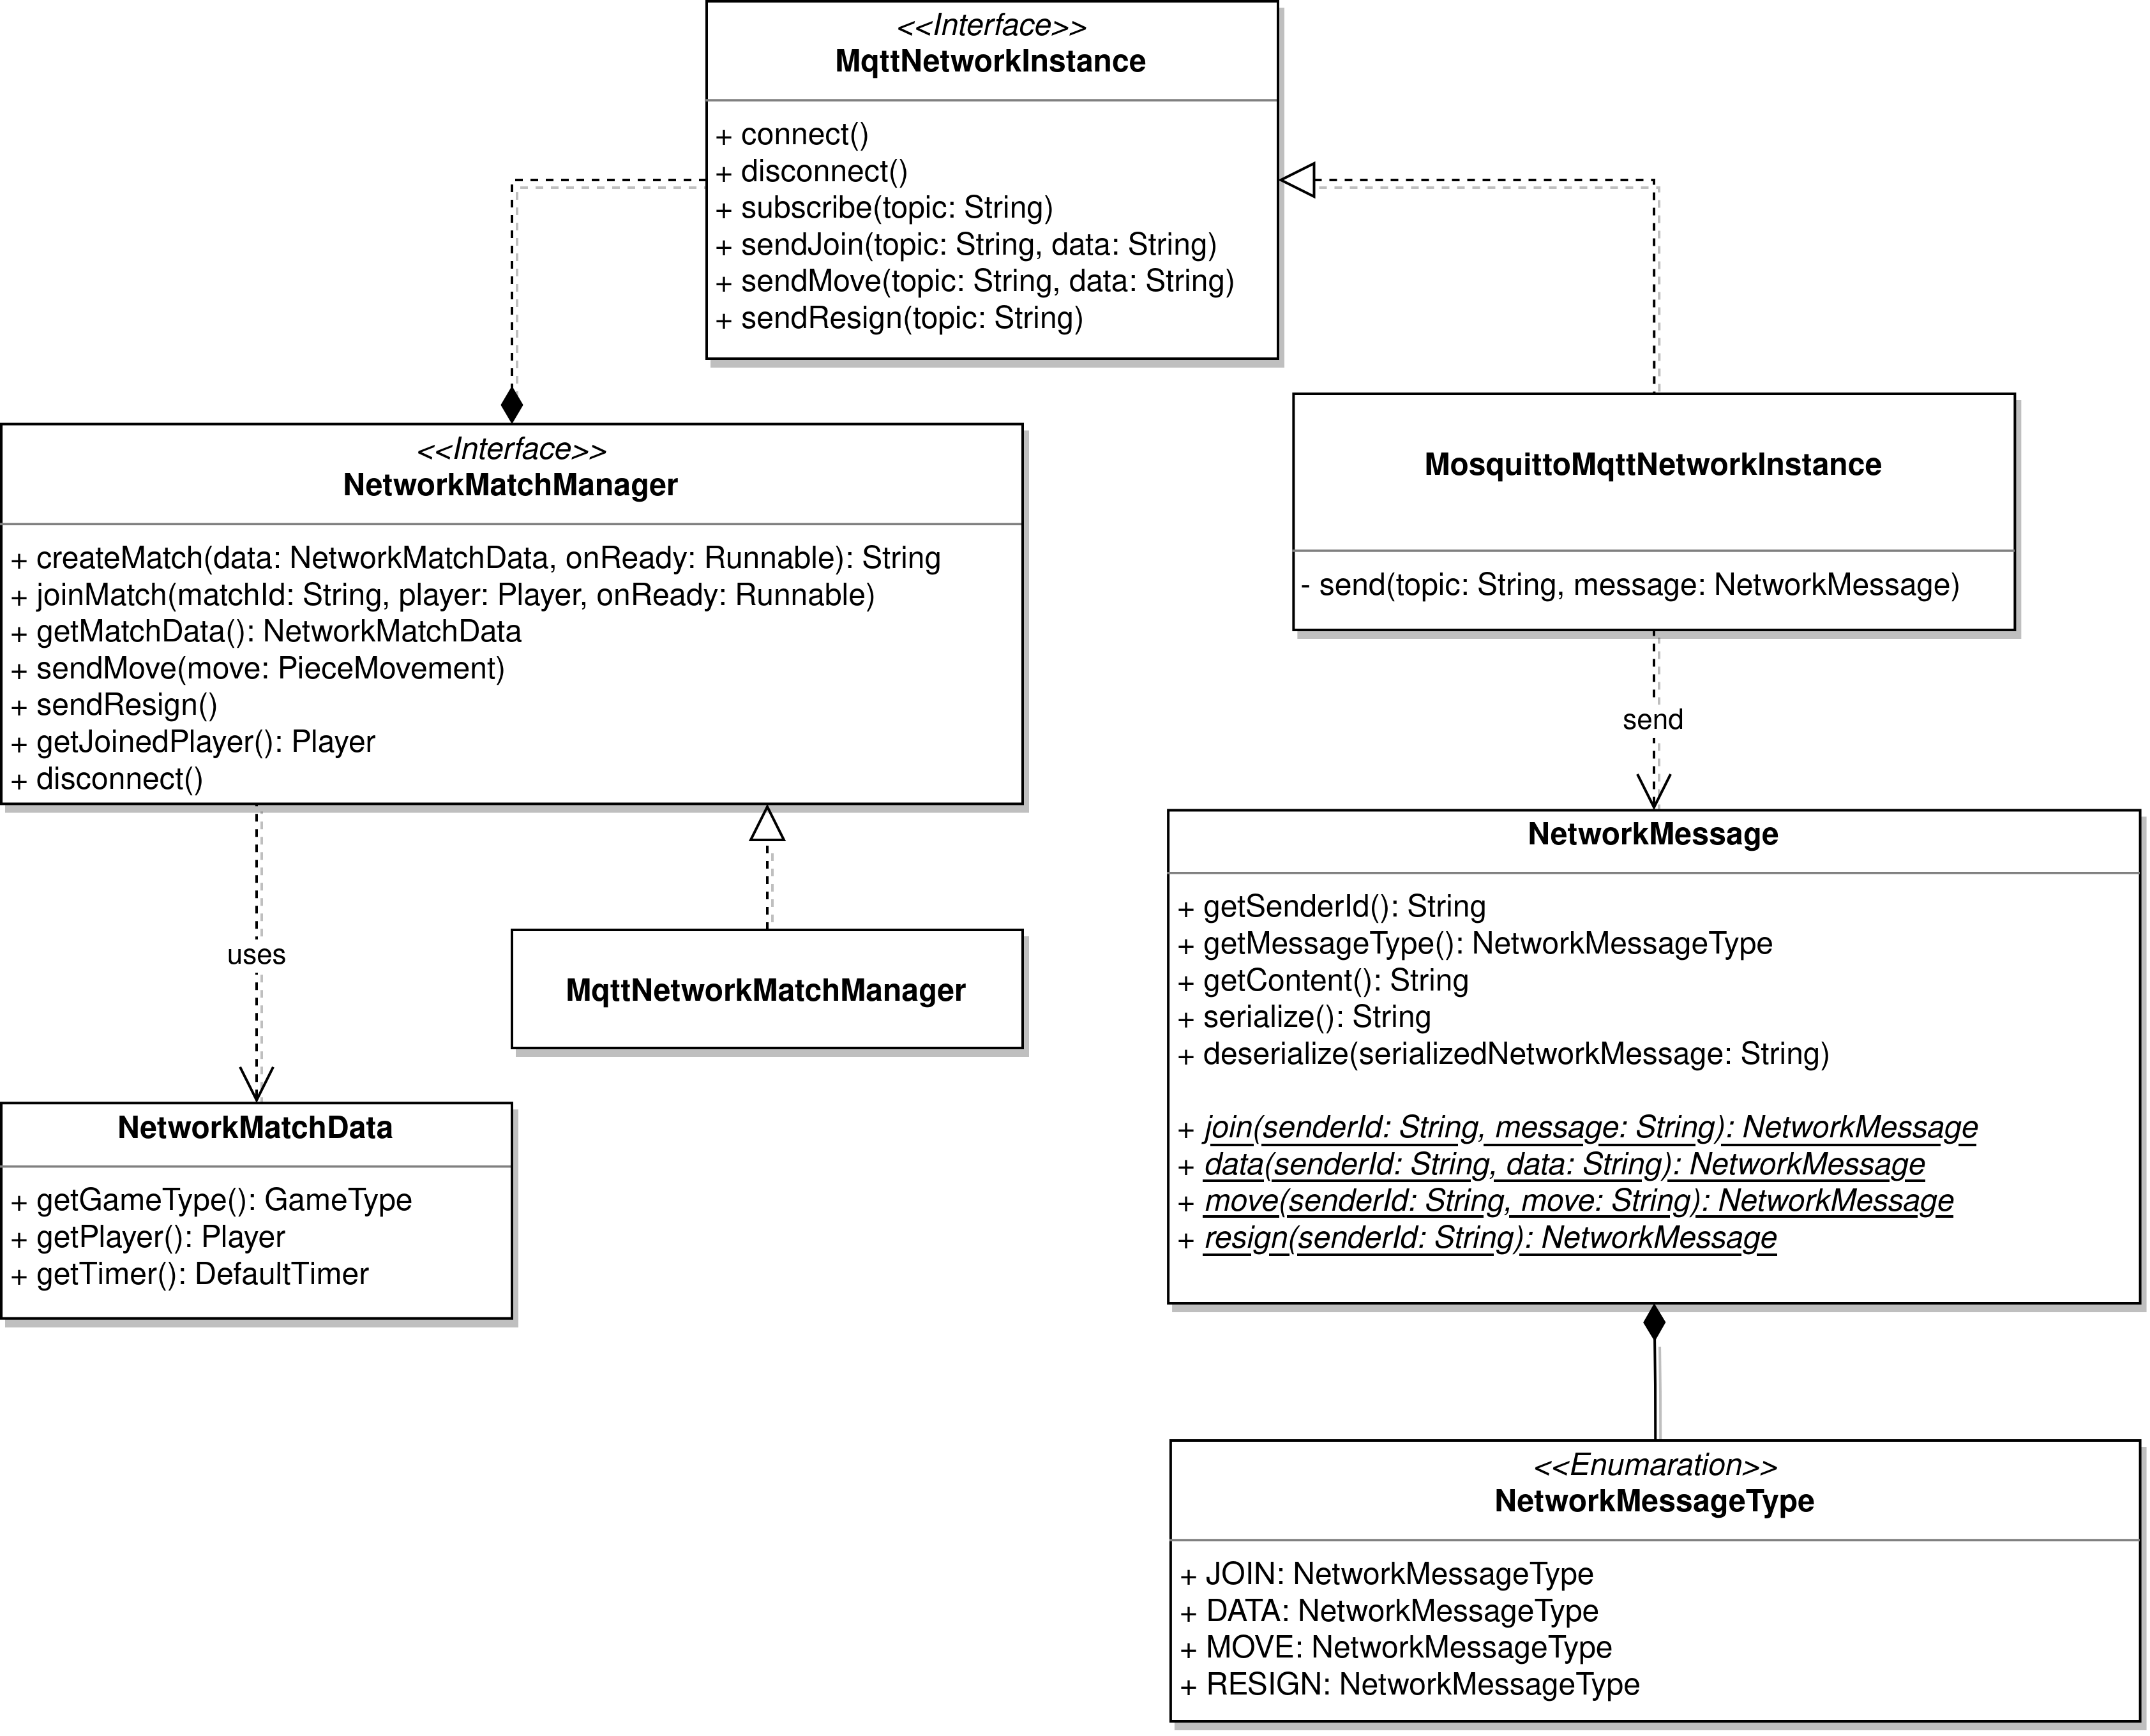
\includegraphics[width=\textwidth]{img/Alessandro/online.png}
    \end{center}
    \caption{Struttura per la gestione della comunicazione via internet tramite protocollo MQTT}
    \label{img:online}
\end{figure}
\
\\
La gestione quindi della modalità online ad un più alto livello è ottenuta tramite l'utilizzo del pattern \textbf{Decorator} mediante l'entità \texttt{OnlineMatch}.
Essa infatti implementa il contratto \texttt{Match} e al suo interno ha un instanza di \texttt{MatchImpl} a cui delega i principali metodi che non richiedono l'invio di messaggi online, mentre quando viene fatta una mossa prima di inviarla al proprio \texttt{Match} interno utilizza il \texttt{NetworkMatchManager} per inviare questa mossa anche all'altro client.
\\
Successivamente invia la mossa anche al proprio Match e restituisce il risultato della mossa all'utente.
\\
Essendo necessario avvisare l'utente del ricevimento di una mossa è stata utilizzata una "callback" mediante la functional interface \texttt{MovementHandler} che permette al controller di specificare cosa fare quando viene ricevuta una mossa.
Infatti quando una mossa viene ricevuta viene inviata al Match interno e ne viene salvato il risultato, questi dati vengono poi passati alla chiamata della callback in modo da poter informare che mossa è stata fatta e che risultato ha avuto.
%
\begin{figure}[H]
    \begin{center}
        \centering
        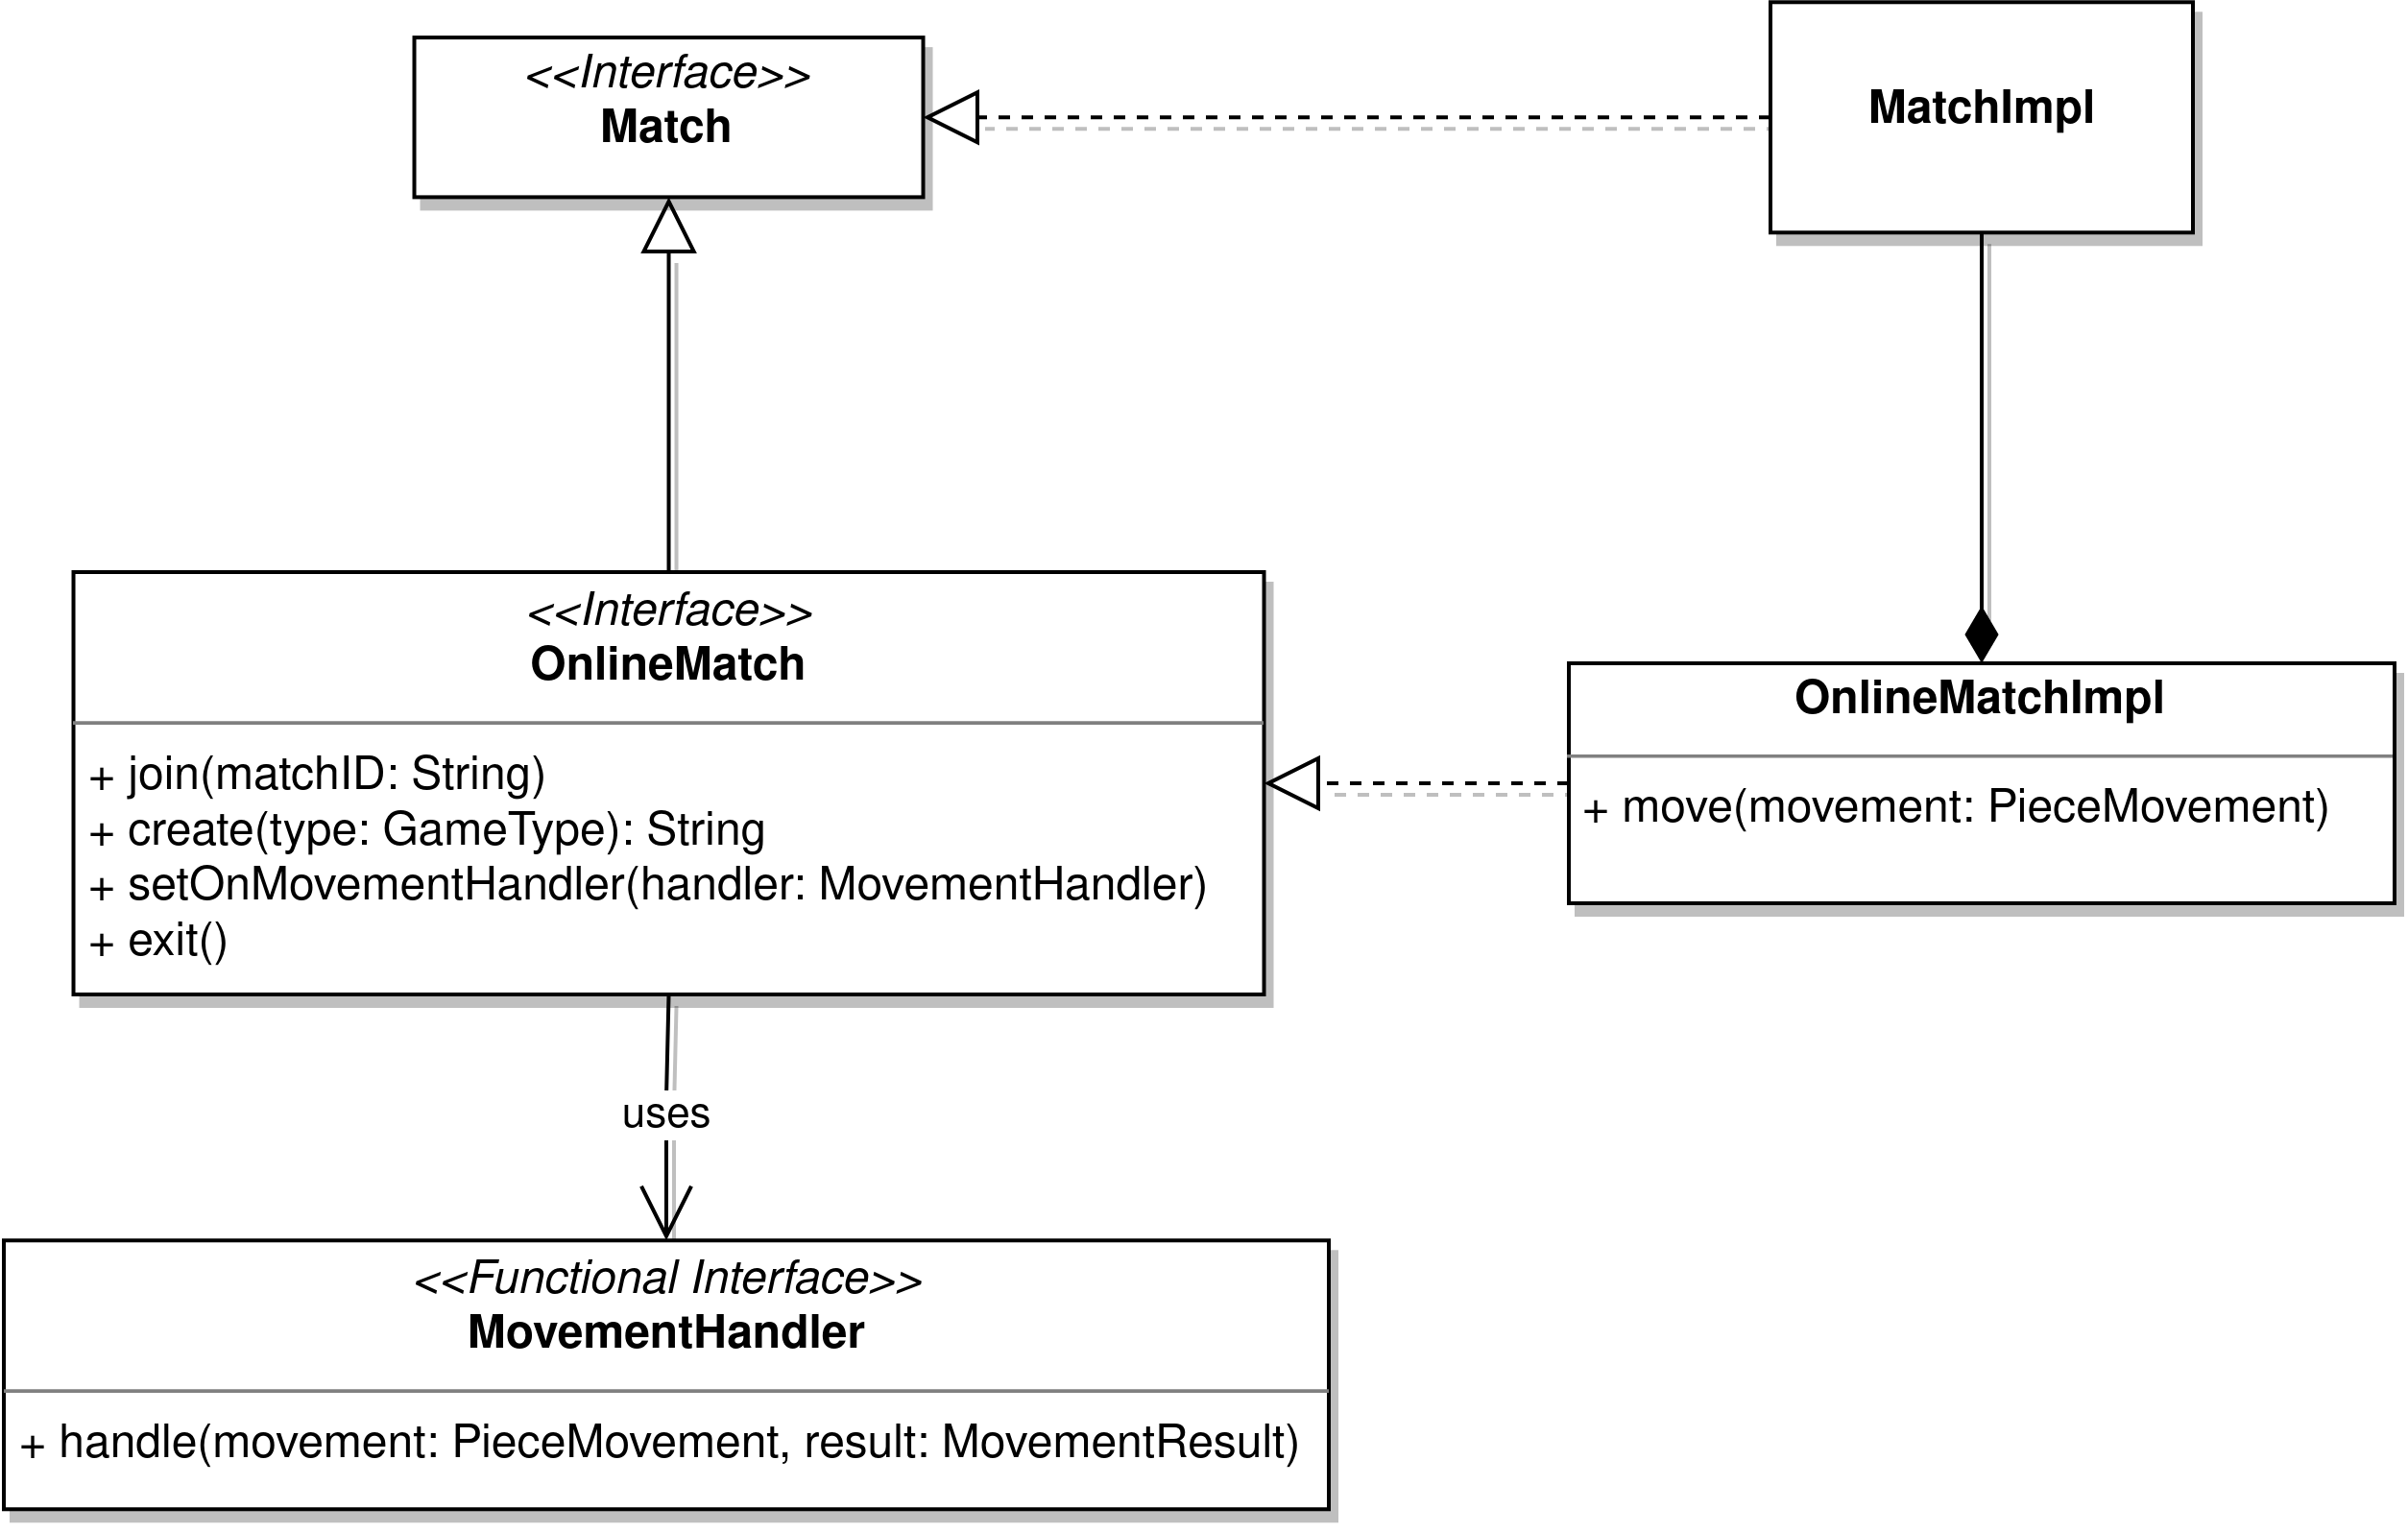
\includegraphics[width=\textwidth]{img/Alessandro/online_match.png}
    \end{center}
    \caption{Gestione del Match online tramite pattern Decorator}
    \label{img:online_match}
\end{figure}

\subsubsection{Graphical Board}
Una volta terminata la mia parte, nel tempo libero, mi sono dedicato al refactoring di quella che era la board a livello grafico che era un po il "core" della parte visiva.
Essa doveva gestire una quantità molto elevata di funzionalità, doveva permettere la visualizzazione dei pezzi, possibilità di movimento tramite trascinamento, navigazione della storia delle mosse tramite digitazione da tastiera e tanto altro...
\\
Quello che ne risultava è che la classe della board era molto grande e poco facilmente gestibile, inoltre avendo vari tipi di board diverse queste erano ottenute tramite un copia/incolla di un altra board opportunamente modificata poiché non erano riutilizzabili.
\\
Tuttavia ciò violava fortemente DRY.
\paragraph{}
\
\\
Ho quindi pensato di fare un breakdown di queste ultime per capire che cosa avevano in comune costruendo quindi quella che è la gerarchia della board.
Ho di conseguenza estratto quello che erano le funzionalità comuni a tutte le board mediante la classe \texttt{GraphicalBoard}, da quest'ultima prendono vita tramite estensione la \texttt{ReplayBoard} e la \texttt{MatchBoard}.
\\
La \texttt{ReplayBoard} è una board che viene utilizzata per la navigazione di una partita salvata, non è quindi necessario avere nessun tipo di movimento dei pezzi da parte dell'utente, mentre è necessario averlo nella \texttt{MatchBoard}, la quale viene utilizzata per giocare una partita. Inoltre essa ha molte altre funzionalità quali la possibilità di evidenziare delle celle e le possibili mosse dei pezzi.
\\
Un ulteriore estensione è la \texttt{OnlineMatchBoard} che deve mettere un vincolo ai movimenti possibili, ovvero l'utente locale che gioca online non può muovere i pezzi del giocatore avversario.
%
\begin{figure}[H]
    \begin{center}
        \centering
        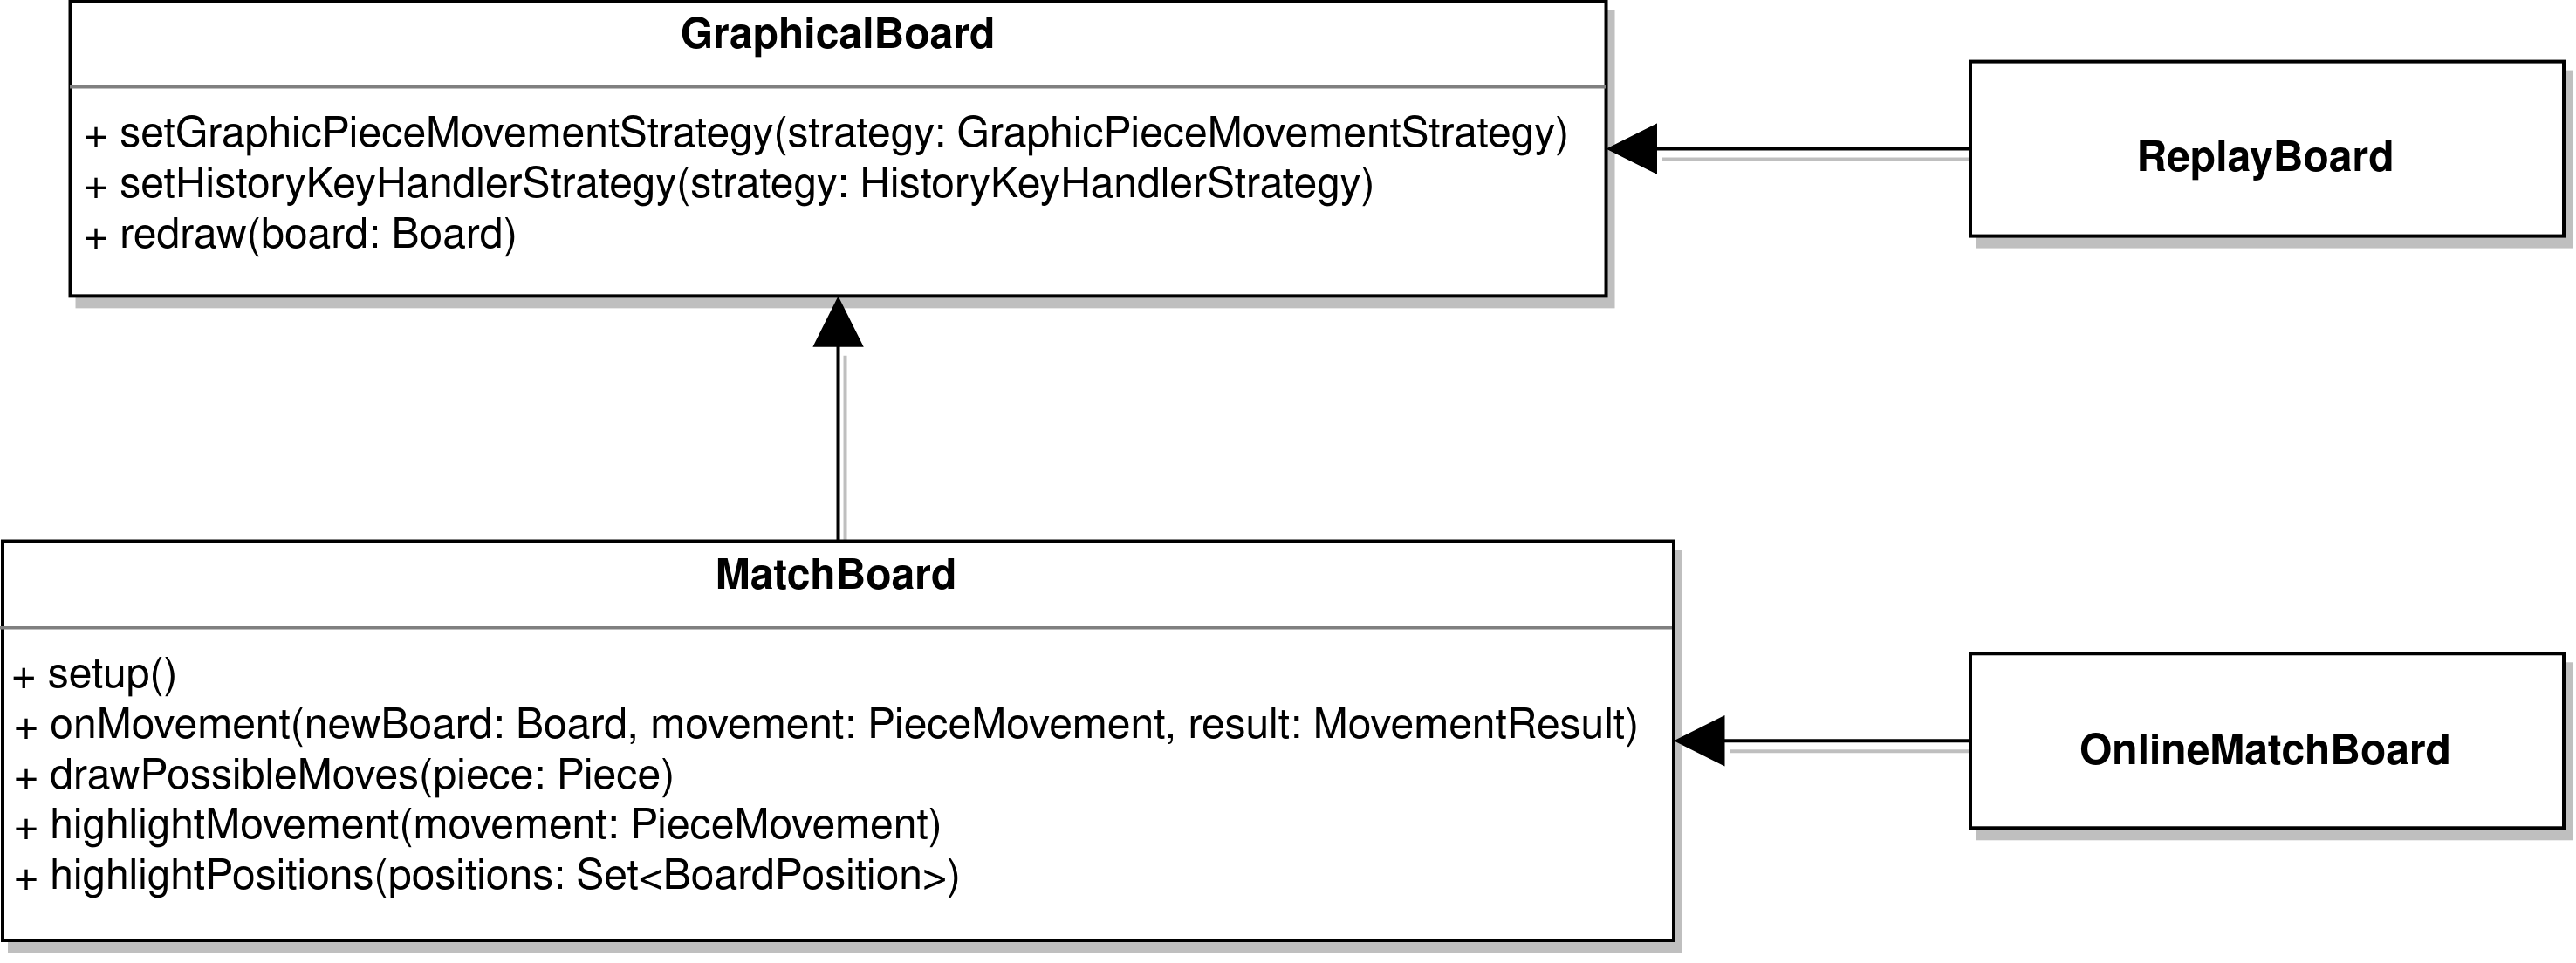
\includegraphics[width=\textwidth]{img/Alessandro/graphic_board.png}
    \end{center}
    \caption{Gerarchie delle varie Board a livello grafico}
    \label{img:graphic_board}
\end{figure}
\
\\
Molto importante è stata la gestione dei movimenti dei pezzi a livello di interfaccia.
Per implementare questa feature ho deciso di utilizzare il pattern \textbf{Strategy} che mi ha permesso di definire un contratto che le varie strategie di movimento dei pezzi dovevano implementare.
\\
Ciò è stato ottenuto tramite l'interfaccia \texttt{GraphicPieceMovementStrategy} che rappresenta appunto la strategia di movimento grafico dei pezzi, il quale si compone di 3 eventi:
\begin{itemize}
    \item Un pezzo viene cliccato
    \item Un pezzo viene trascinato
    \item Un pezzo viene rilasciato
\end{itemize}
Ciò mi ha permesso di definire appunto una struttura generale del contratto di movimento dei pezzi a livello grafico e ne sono giunte di conseguenza le implementazioni per una normale partita tramite la \texttt{NormalMatchGraphicPieceMovementStrategy} e la sua derivata \texttt{OnlineMatchGraphicPieceMovementStrategy} che come già detto precedentemente non deve dare all'utente locale la possibilità di muovere i pezzi dell'avversario.
\\
Poichè questa strategia di movimento dei pezzi è stata resa parte dalla classe base
\texttt{GraphicalBoard}, ovvero tutte le board la hanno, è stata necessaria e molto semplice la creazione della classe \texttt{NonMovableGraphicPieceMovementStrateg}y che viene usato nelle board come la \texttt{ReplayBoard} in cui il movimento dei pezzi non è permesso.

%
\begin{figure}[H]
    \begin{center}
        \centering
        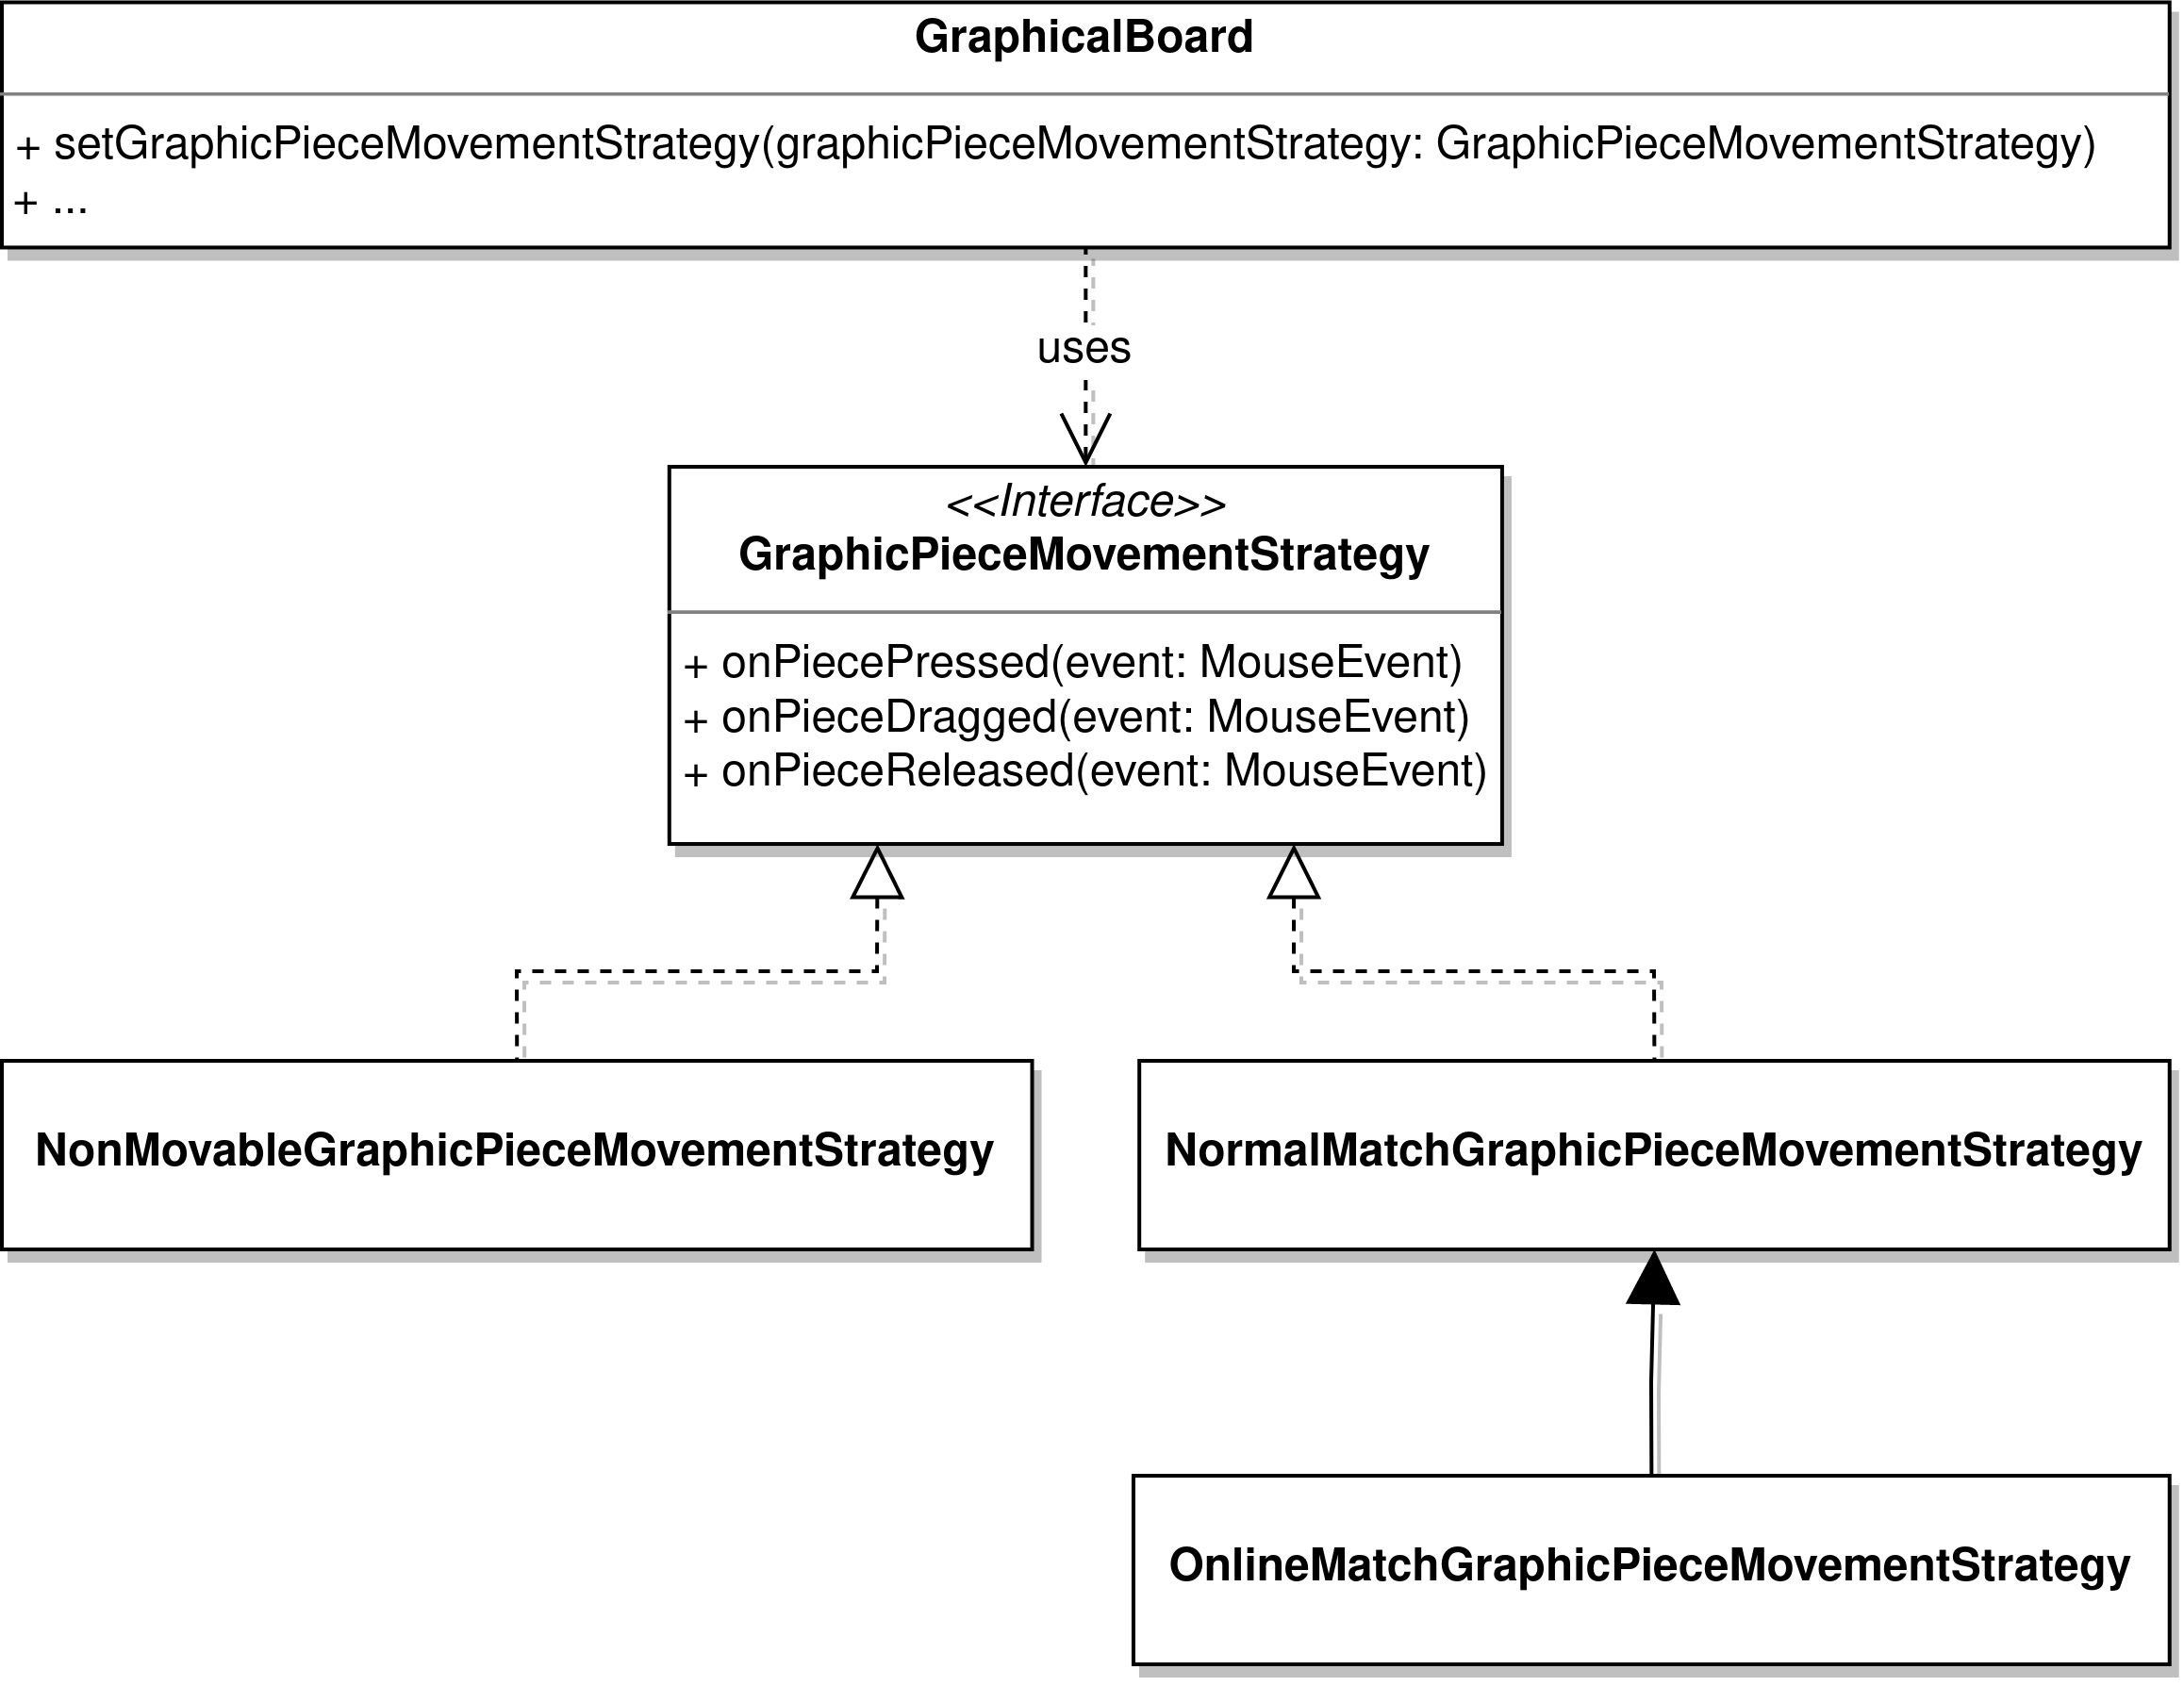
\includegraphics[width=\textwidth]{img/Alessandro/graphical_piece_movement_strategy.png}
    \end{center}
    \caption{Strategia per il movimento dei pezzi a livello grafico}
    \label{img:graphical_piece_movement_strategy}
\end{figure}
%
\
\\
Altra necessità che molte board avevano in comune era la possibilità di navigare le mosse precedenti.
Anche in questo caso ho deciso di utilizzare il pattern \textbf{Strategy} tramite la \texttt{HistoryKeyHandlerStrategy}, ovvero la strategia che definisce cosa fare quando viene premuto un tasto sulla tastiera da parte dell'utente.
\\
È stato dunque molto semplice gestire analogamente alla
\texttt{GraphicPieceMovementStrategy} due semplici strategie di navigazione della \texttt{History}, una che prevede una normale navigazione tramite le frecce (\texttt{NormalHistoryKeyHandlerStrategy}) e un altra che invece non rende possibile la navigazione (\texttt{NonNavigableHistoryKeyHandlerStrategy}) adottata in quelle board che non hanno bisogno della navigazione della storia delle mosse. 
%
\begin{figure}[H]
    \begin{center}
        \centering
        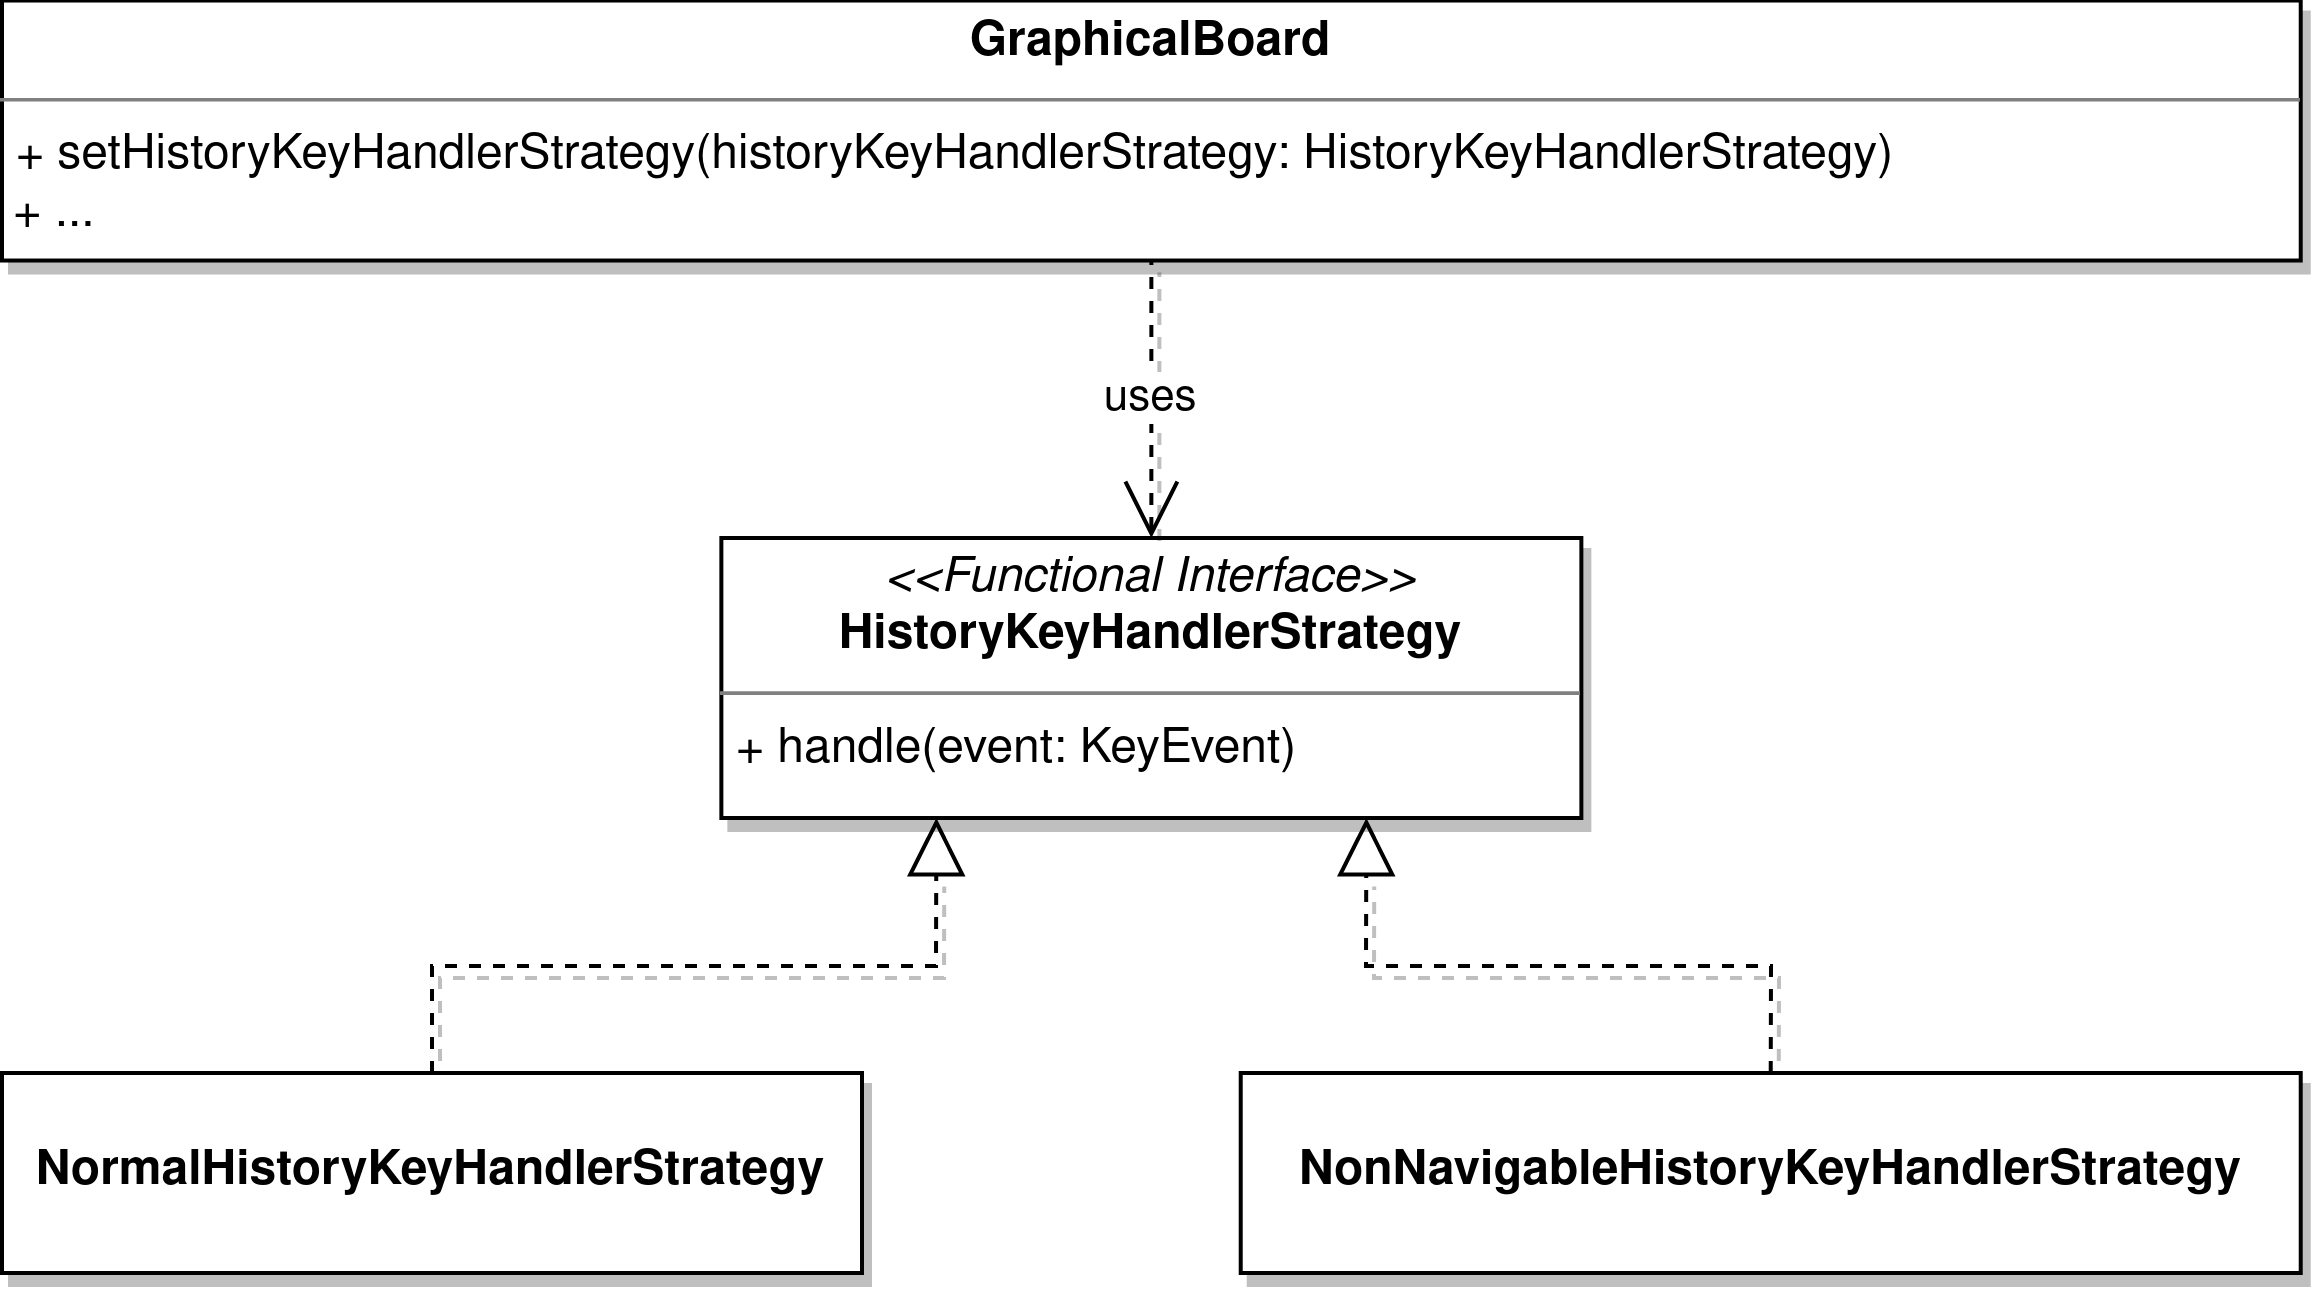
\includegraphics[width=\textwidth]{img/Alessandro/history_key_strategy.png}
    \end{center}
    \caption{Navigazione della History di una partita mediante pattern Strategy per l'handling del click dei tasti}
    \label{img:history_key_strategy}
\end{figure}

\clearpage
\subsection{Tommaso Patriti}

\subsubsection*{Replay}
\texttt{Replay} serve per mantenere uno storico con la cronologia delle mosse delle partite giocate con Jhaturanga, è implementato in tutte le sue versioni: classica, varianti, online e scacchiera personalizzata.
\begin{figure}[H]
    \begin{center}
        \centering
        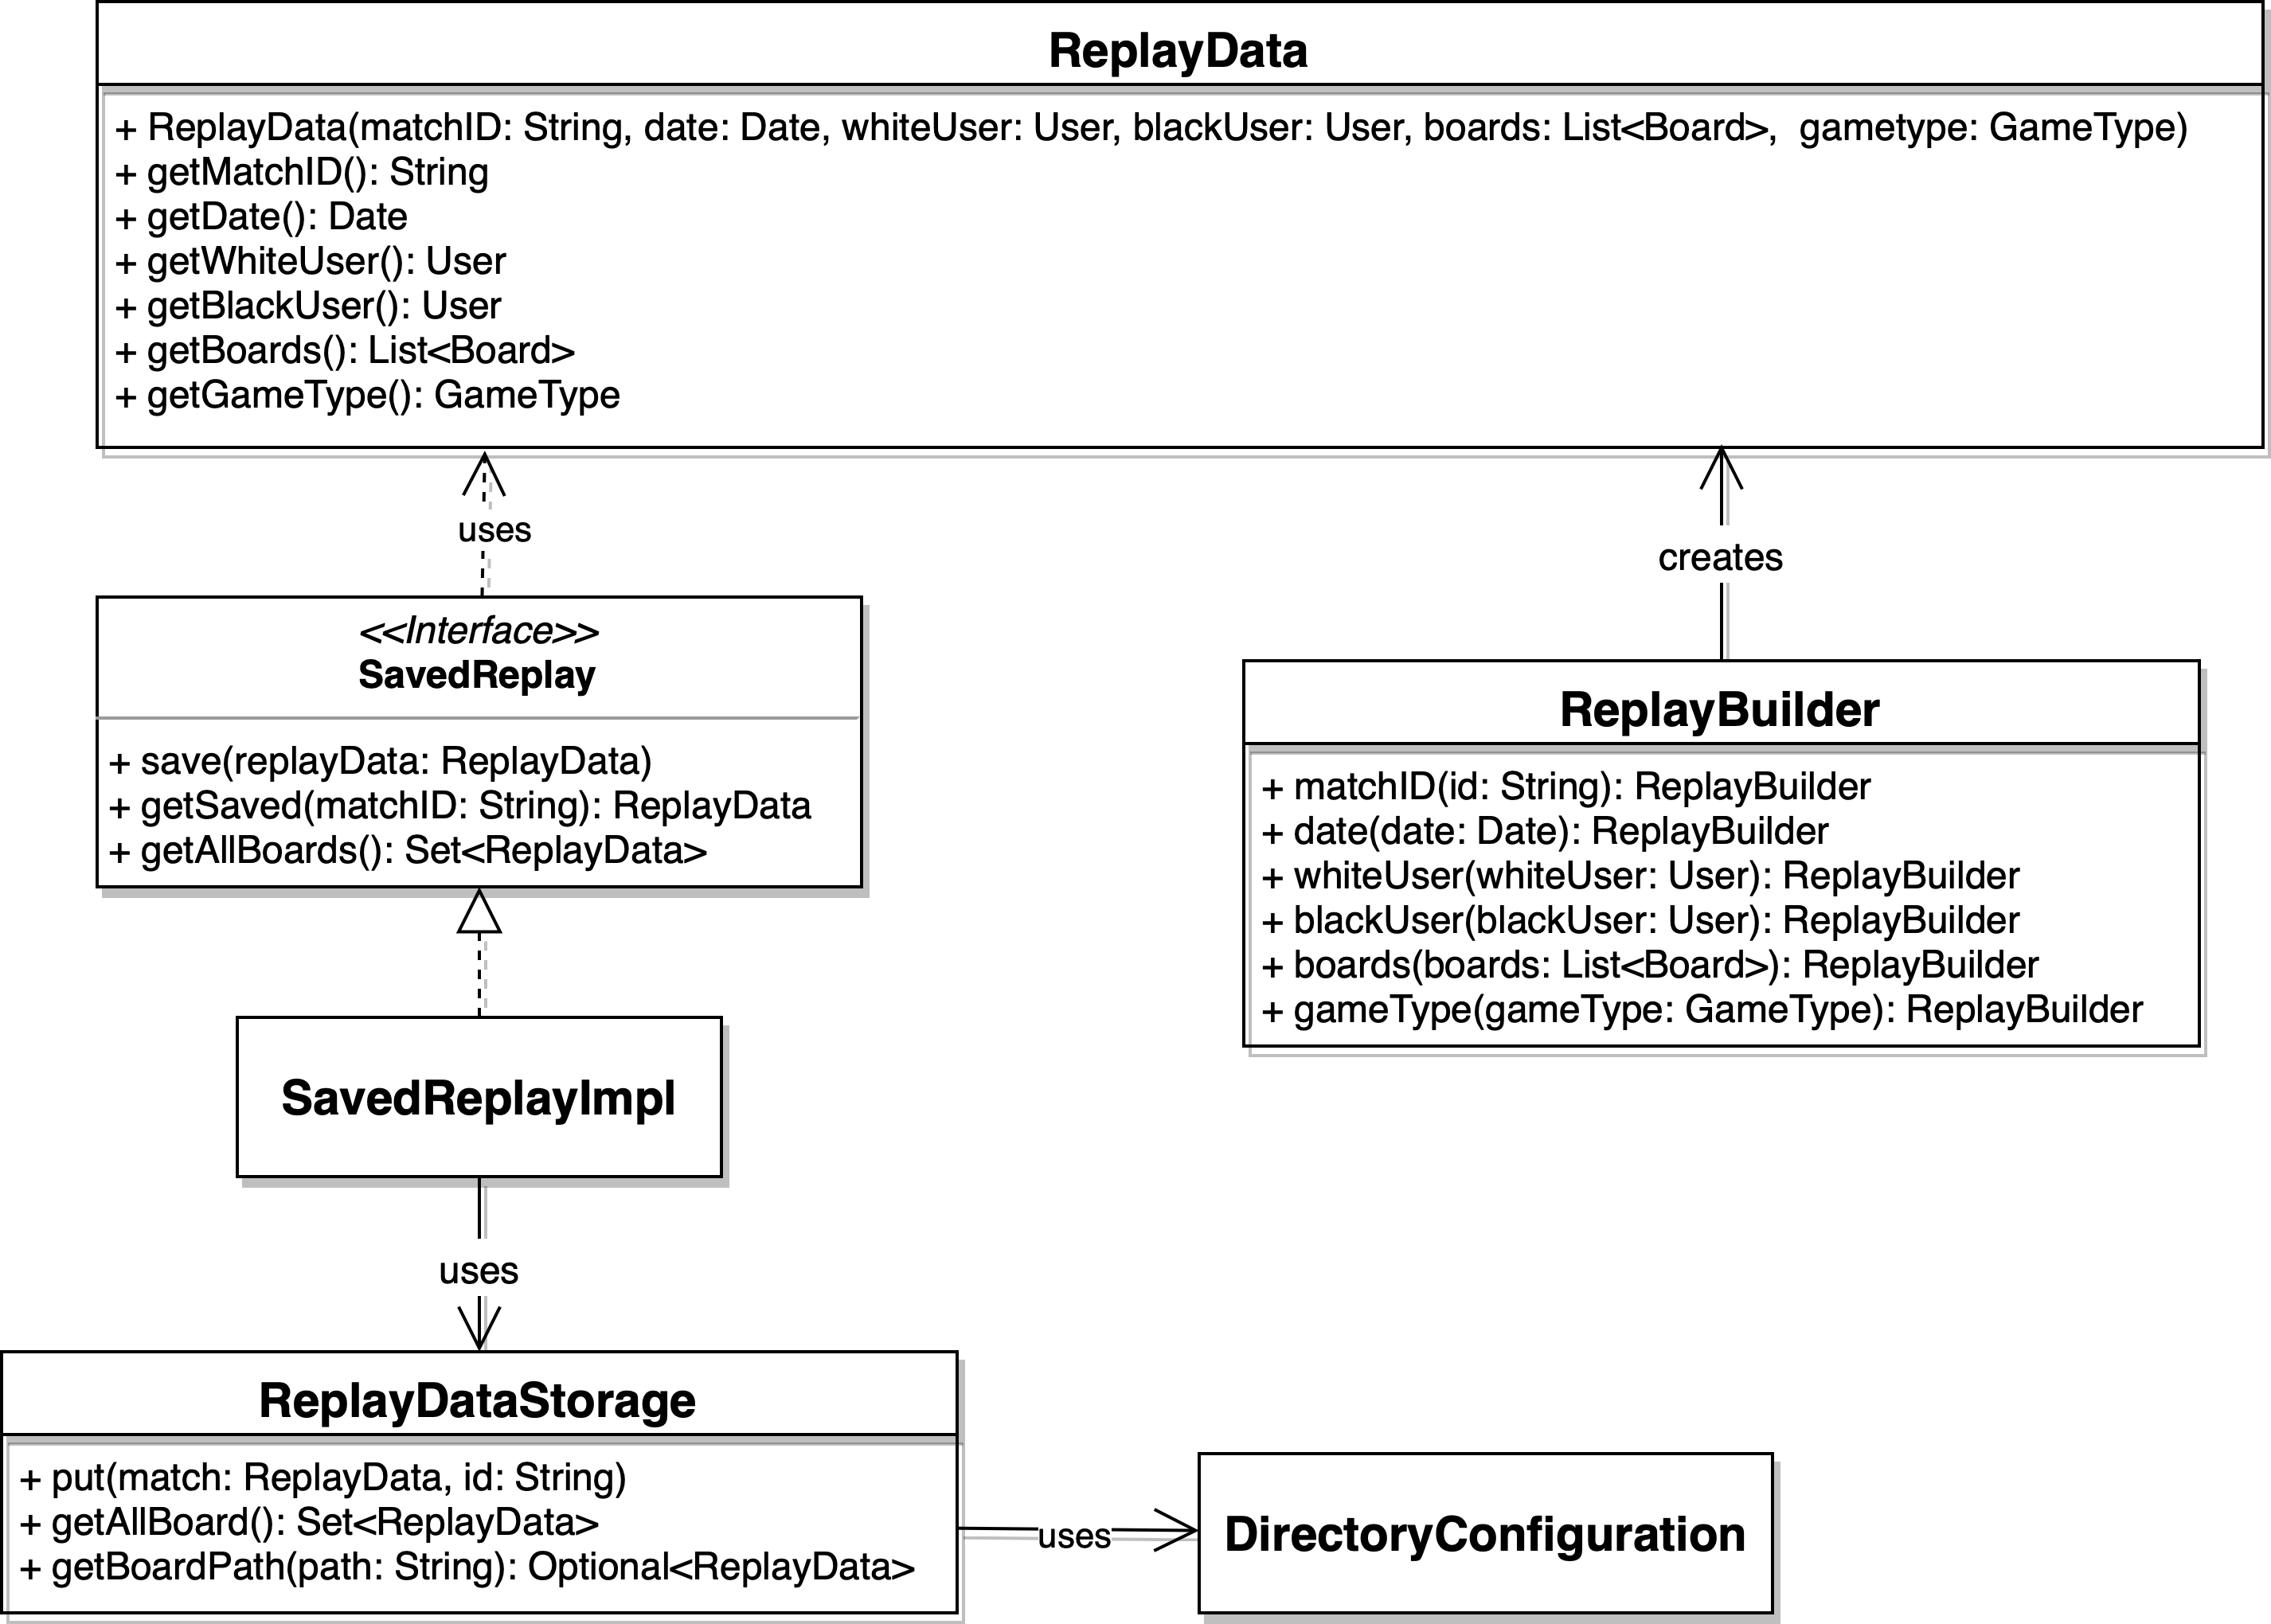
\includegraphics[width=\textwidth]{img/Tommaso/replay.png}
    \end{center}
    \caption{Gestione salvataggio partite e Replay}
    \label{img:replay}
\end{figure}
\
\\
\texttt{ReplayData} è una classe che contiene tutte le informazioni necessarie per il salvataggio di una partita.\\
Considerando i numerosi campi necessari alla sua creazione, ho deciso di implementare il pattern \textbf{Builder}.\\
\texttt{ReplayData} è un oggetto seralizable in maniera tale da poter essere salvato e riutilizzato agevolmente.\\
\texttt{ReplayDataStorage}, si occupa di comunicare con la cartella .jhaturanga utilizzata per il salvataggio dei file permanenti dell'applicazione.\\
La gestione della cartella .jhaturnaga è implementata in DirectoryConfiguration, che è condivisa da tutti gli oggetti che hanno necessità di accedere a file salvati nel computer. .jhaturanga è una cartella che si trova nella home directory in cui viene eseguita l'applicazione.
SavedReplay si occupa di gestire la comunicazione tra ReplayDataStorage e il resto dell'applicazione, in maniera tale da avere sempre un corretto utilizzo dei file.

\subsubsection*{Timer}
Il \texttt{Timer} è un oggetto che serve per la gestione del tempo durante una partita di scacchi.
\begin{figure}[H]
    \begin{center}
        \centering
        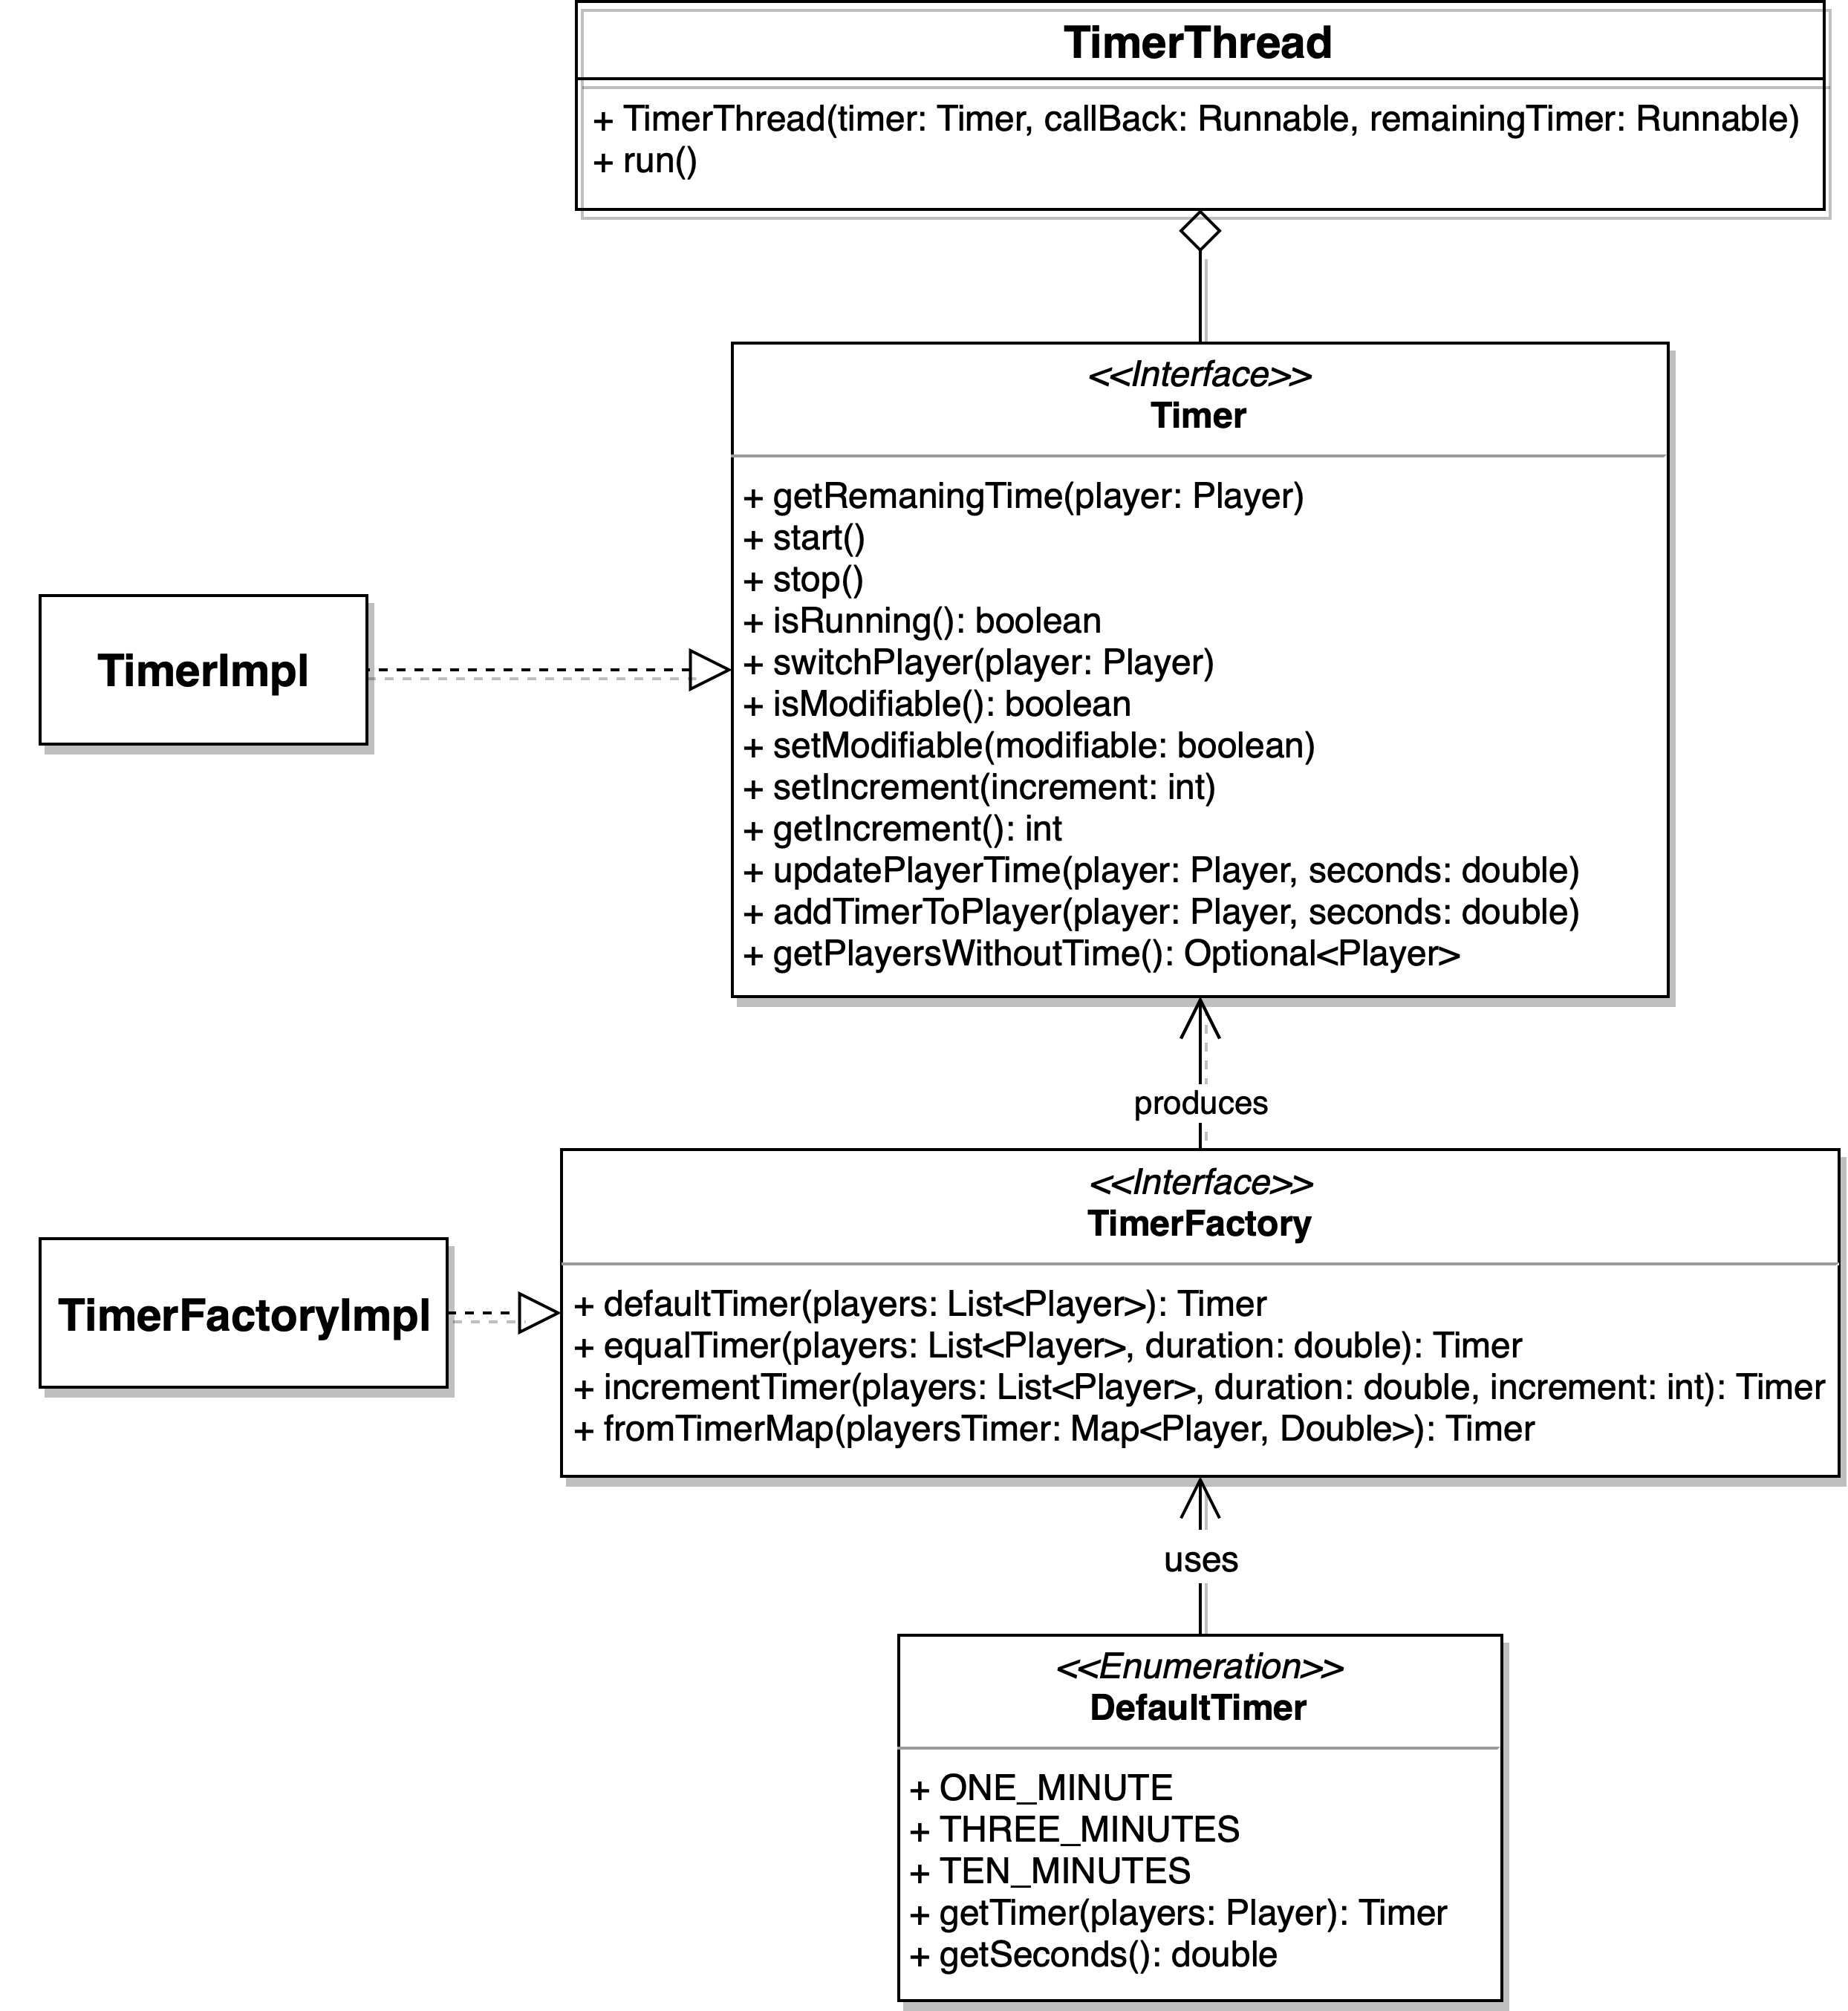
\includegraphics[scale=0.75]{img/Tommaso/timer.png}
    \end{center}
    \caption{Gestione Timer}
    \label{img:timer}
\end{figure}
\
\\
Il \texttt{Timer} è un oggetto che tiene in memoria la lista dei giocatori e il tempo loro rimanente.
È stato implementato il pattern \textbf{Factory} per poter avere a disposizione varie tipologie di distribuzione del tempo.
Visto che negli scacchi si usano dei timer ricorrenti, ho deciso di dichiarare questi ultimi all'interno dell'enum DefaultTimer.
Il Timer deve funzionare indipendentemente rispetto alle operazioni svolte sulla scacchiera, quindi serve un thread separato per gestirlo. Inizialmente quest'ultimo era direttamente implementato nella view, ma ciò portava side-effects nel suo utilizzo quindi ho implementato TimerThread che estende Thread, e richiama l'applicazione ogni volta che aggiorna il suo stato e quando uno dei partecipanti finisce il tempo. Questo viene fatto tramite la FunctionalInterface Runnable.

\subsubsection*{Audio}
Semplice classe con metodi statici per gestire l'audio
\begin{figure}[H]
    \begin{center}
        \centering
        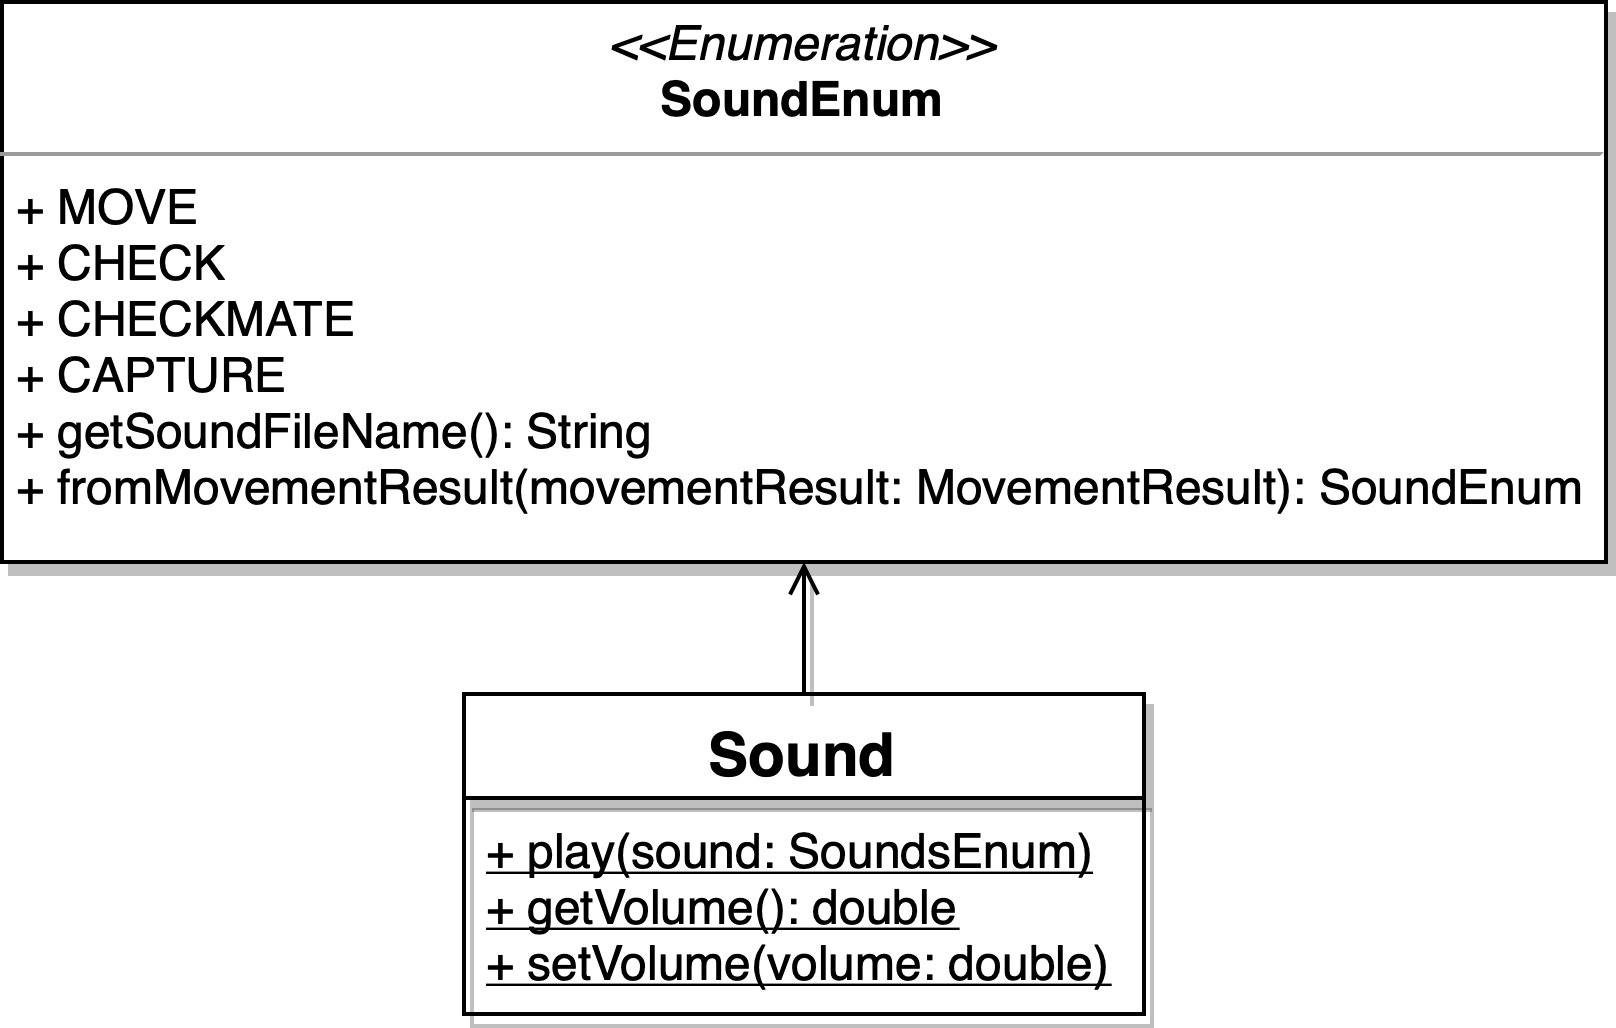
\includegraphics[scale=0.75]{img/Tommaso/sound.png}
    \end{center}
    \caption{Gestione del suono}
    \label{img:sound}
\end{figure}
\paragraph{}
\subsubsection*{Style}
La gestione degli stili è stata sviluppata affinché l'applicazione ne abbia di default da poter selezionare. É implementata anche la possibilità di aggiungerne di nuovi, potendo quindi personalizzare quelli esistenti.
\begin{figure}[H]
    \begin{center}
        \centering
        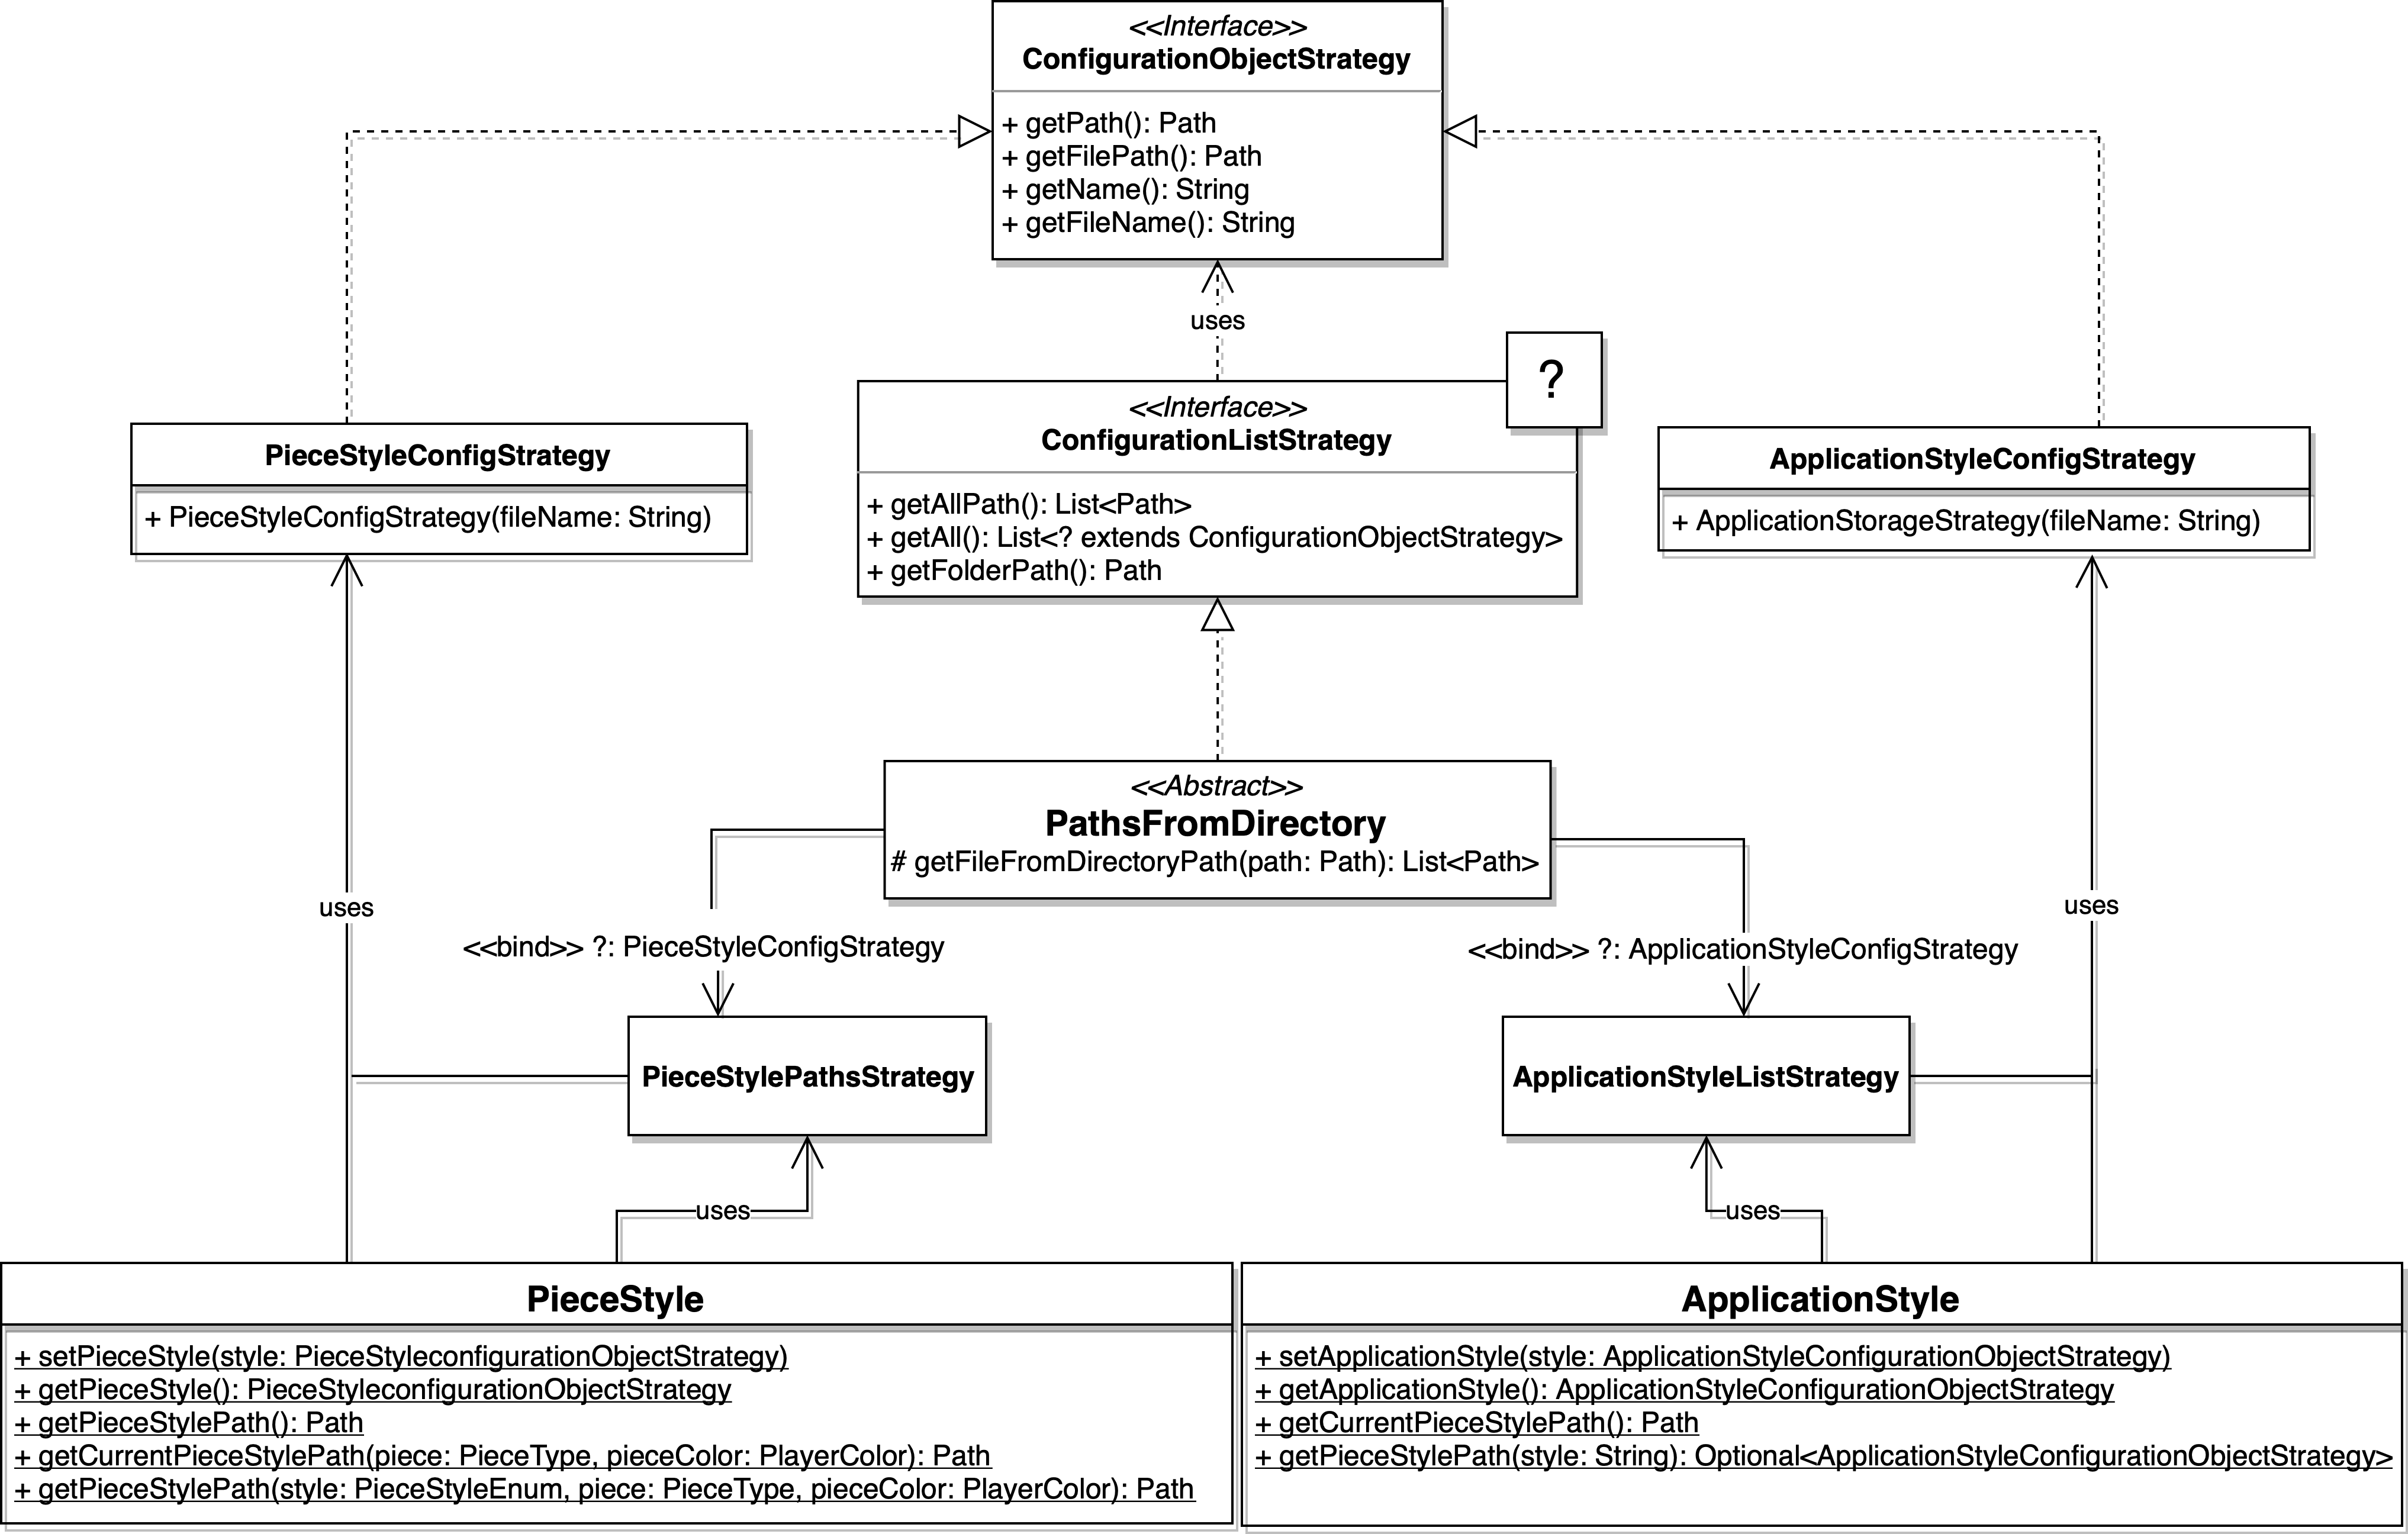
\includegraphics[width=\textwidth]{img/Tommaso/style.png}
    \end{center}
    \caption{Gestione degli stili}
    \label{img:style}
\end{figure}
\
\\
%
\texttt{PieceStyle} gestisce lo stile di tutti i pezzi della scacchiera cambiando il percorso della cartella in cui si trovano. 
In caso non ci siano stili preferiti, la classe ne prevede uno di default.
\\
\texttt{ApplicationStyle} gestisce i fogli di stile (CSS) usati da JavaFx.
In caso non ci siano stili preferiti, la classe ne prevede uno di default.
Queste due classi hanno una gestione simile, quindi a prima vista sarebbe possibile andarle a gestire con un eventuale \textbf{Template Method} implementato per mezzo dei tipi generici. Ho deciso di non seguire questa strada poiché l'utilizzo delle due classi è differente e le righe di codice in comune sono esigue, quindi, andandone a generalizzare l'utilizzo, avrei sacrificato la chiarezza del codice e portato ad un limitato incremento di flessibilità.
Queste due classi per funzionare hanno bisogno di avere a disposizione una lista di stili.
Inizialmente li ricavavano da una classe Enum, ma questo comprometteva l'estensibilità del codice, quindi ho deciso di eliminare queste ultime e creare delle liste di stili dipendenti dalle risorse disponibili in .jhaturanga.
All'interno di quest'ultima in res/piece possiamo aggiungere cartelle contenenti le immagini degli scacchi, e in /res/css/thems, file css, per lo stile dell' applicazione.

Per gestire queste risorse, ho deciso di utilizzare \textbf{Strategy} in due punti:
\begin{itemize}
    \item  \texttt{ConfigurationObjectStrategy} serve per creare degli oggetti che rappresentano gli stili, quindi, serve a contenere i loro percorsi, e dei metodi utili alla manipolazione specifica di questi ultimi.
    \item \textit{ConfigurationListStrategy} serve a contenere tutte le istanze disponibili di \texttt{ConfigurationObjectStrategy}, quindi, in pratica, la lista degli stili disponibili.
    \texttt{PathFormDirectoy} è una classe astratta che si frappone tra \texttt{ConfigurationObjectStrategy} e le sue implementazioni, e fornisce metodi utili alla lettura e scrittura delle resorse.
\end{itemize}
\paragraph{}


\subsubsection*{Setting}
Setting serve per gestire le personalizzazioni scelte dall'utente e si occupa di mantenerle sul computer in maniera tale da averle permanentemente salvate.
\begin{figure}[H]
    \begin{center}
        \centering
        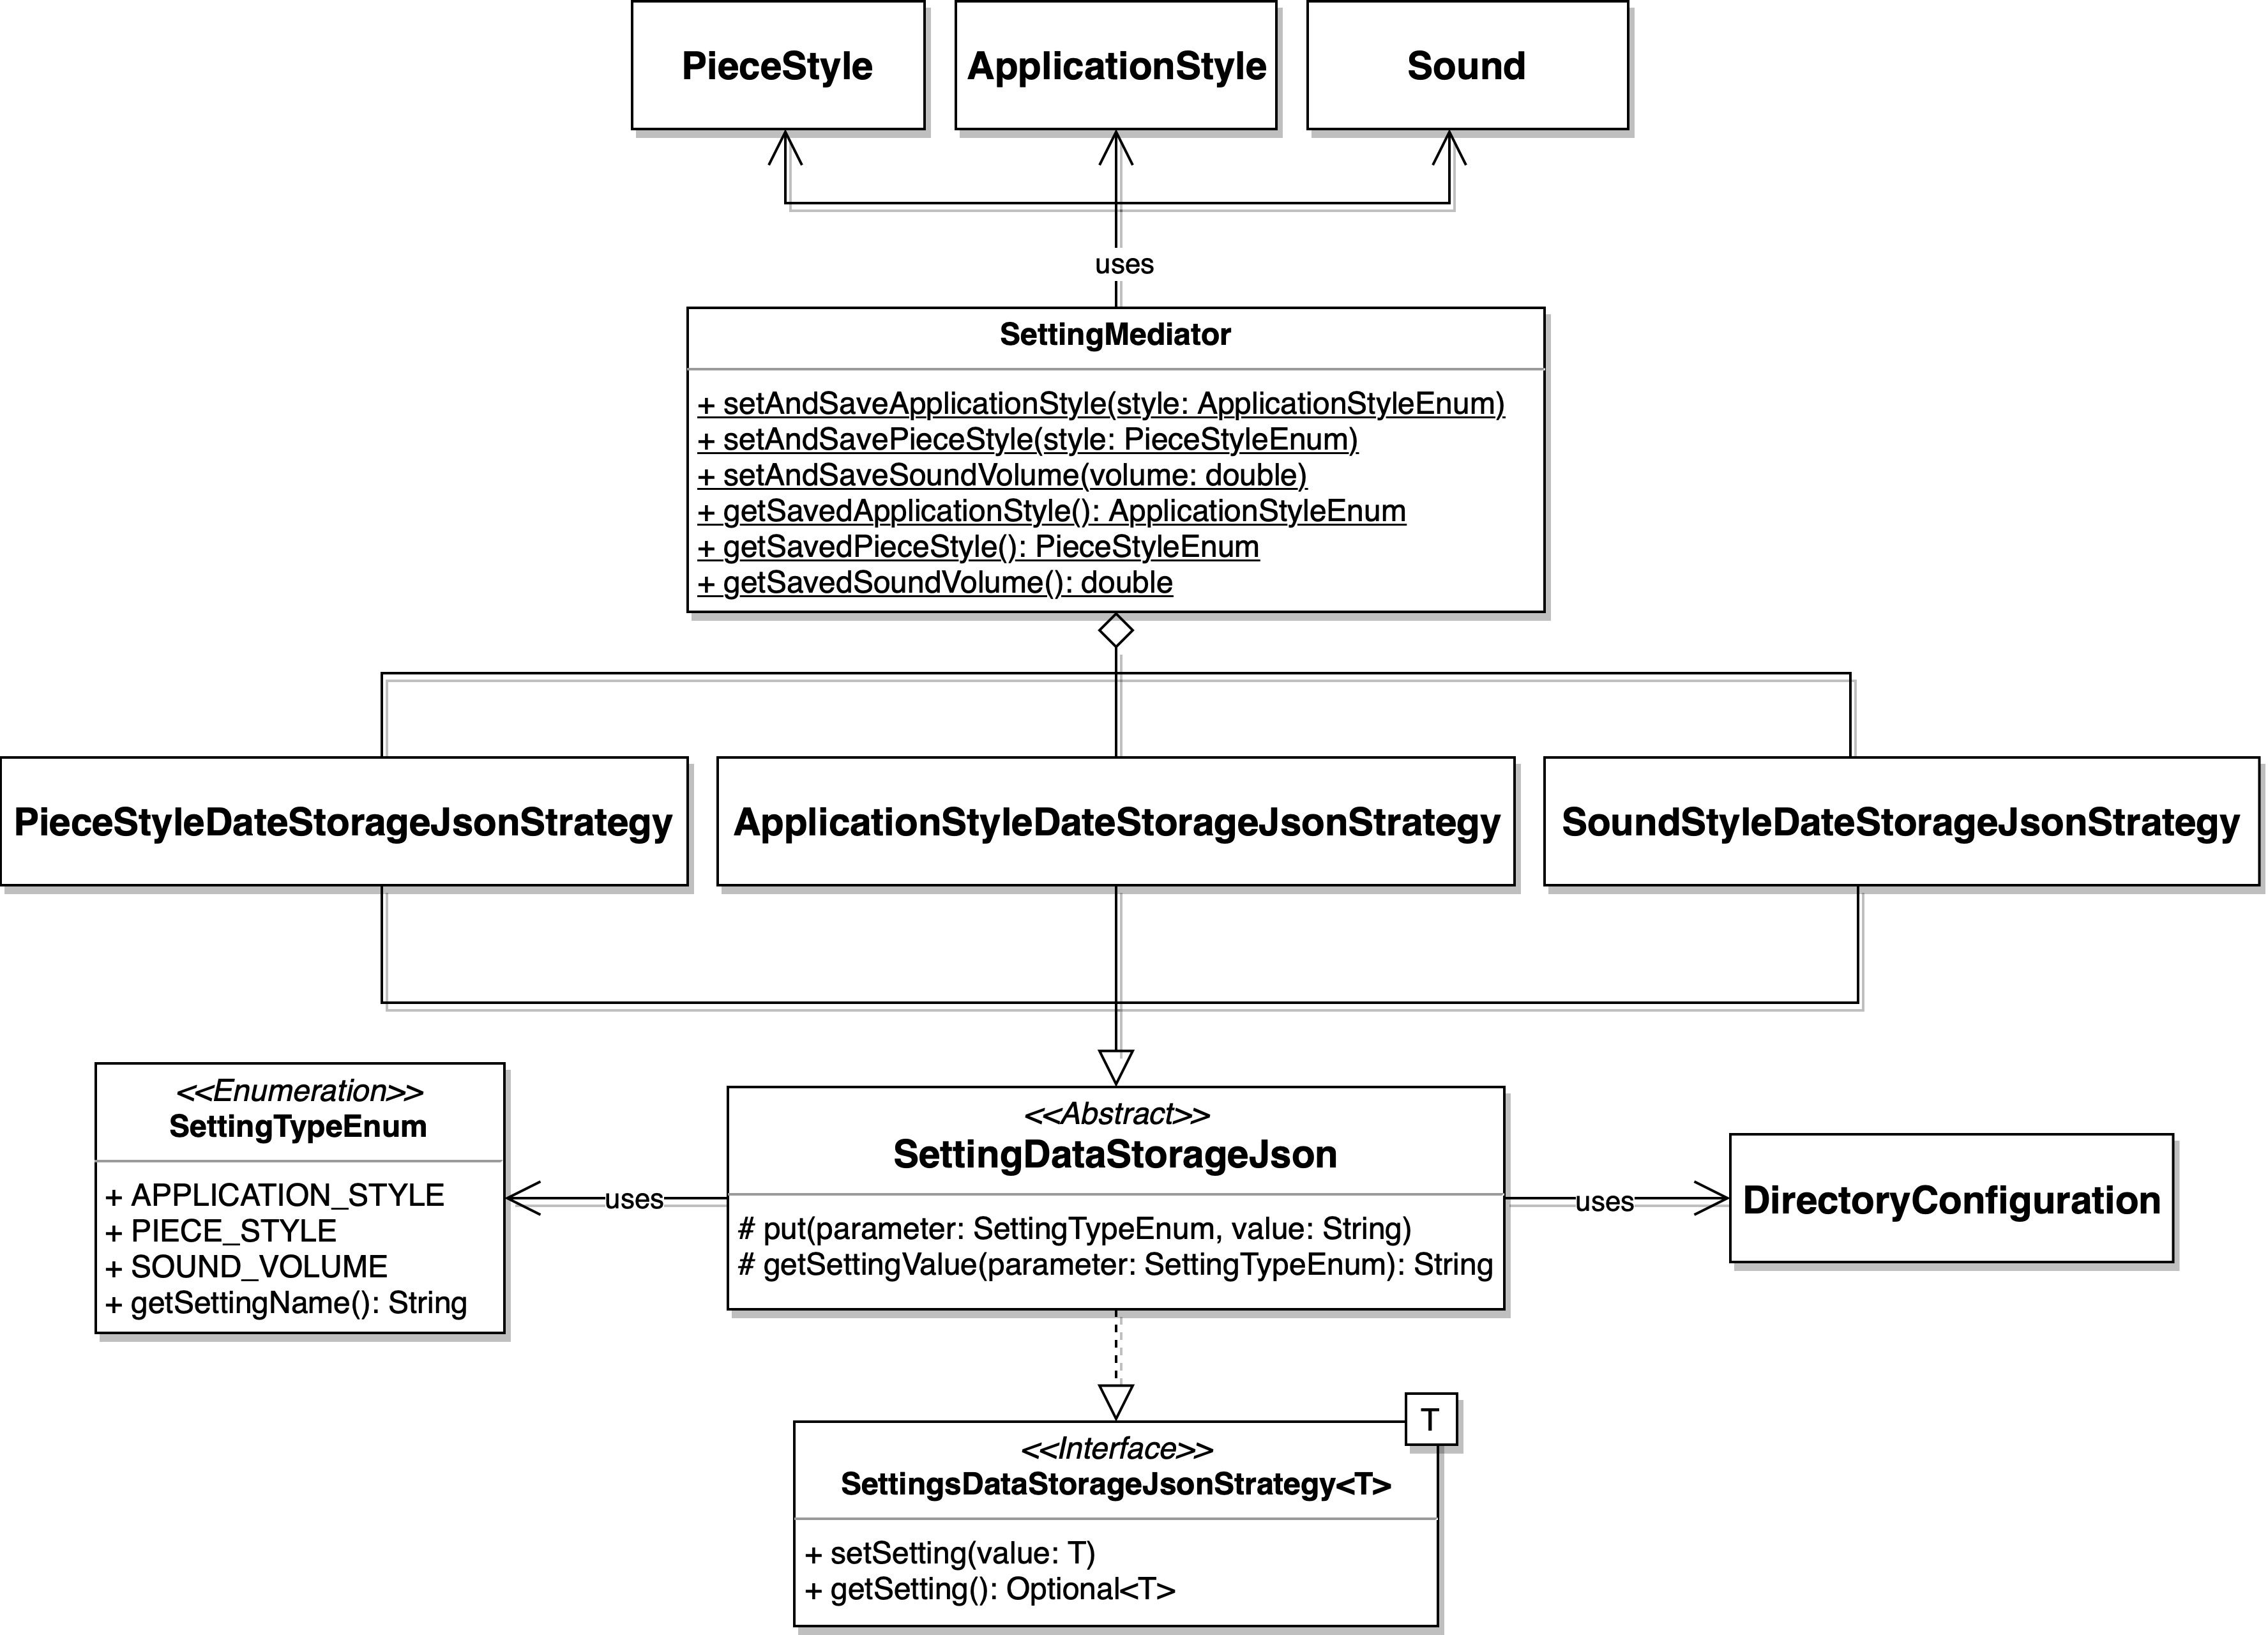
\includegraphics[width=\textwidth]{img/Tommaso/settings.png}
    \end{center}
    \caption{Gestione dei setting}
    \label{img:settings}
\end{figure}
\
\\
L'obiettivo di questa parte di progetto è quello di poter salvare permanentemente le impostazioni preferite dall'utente.\\
Ho deciso di mantenere separata la gestione del salvataggio dalla parte di configurazione.
SettingDataStorageJsonStrategy è un' interfaccia che serve per l'implementazione del pattern \textbf{Strategy}. Ho stabilito di usare strategy in quanto le operazioni da fare sul file json sono sempre uguali, cambia solo l'interpretazione dei dati al momento della lettura e della scrittura. 
Pertanto, ad ogni configurazione corrisponde una classe che ne permette il salvataggio, ma che opera in maniera indipendente dalla classe di configurazione vera e propria.\\
Poiché in questo modo l'entità per il salvataggio delle configurazioni e le entità per la gestione delle configurazioni erano disgiunte, ho deciso di implementare settingMediator che usa il pattern \textbf{Mediator} per avere un'unica classe statica a cui accedere dal resto dell'applicazione che va a gestire l'interazione tra gestione e salvataggio delle impostazioni.
Inoltre ho deciso di frapporre una classe astratta SettingDataStorageJson per avere dei metodi per la gestione del file Json in tutte le classi che hanno stretto un contratto con SettingDataStorageStrategy
La lista dei parametri gestiti dai settings è fornita da SettingTypeEnum.
Inizialmente SettingDataStorageStrategy per evitare problemi di scrittura nel json, era implementata per mezzo di stringhe, ma, per rendere il codice più espressivo e immediato da usare, ho deciso di optare per i generici, in modo tale che nelle ramificazioni di Strategy si possa decidere in libertà come gestire il parametro che verrà poi scritto e letto nel file json.


\clearpage
\subsection{Scolari Stefano}

Fin dalle fasi di analisi uno tra i nostri principali obiettivi era quello di creare un applicativo in grado di gestire un numero molto elevato di varianti scacchistiche.
\\
La sfida principale da me affrontata è stata quindi la realizzazione di un'architettura di base il quanto più estendibile possibile, sia dal punto di vista dei movimenti dei singoli pezzi gestiti dalla \texttt{PieceMovementStrategies}, sia per quanto riguarda le regole che governano le varie modalità di gioco, queste ultime gestite sia dal \texttt{GameController} che dal \texttt{MovementManager}.\\
Adotterò un approccio bottom-up per descrivere il design dell' architettura da me implementata, tracciando e descrivendo quelli che sono i layer attraverso cui ho deciso di stratificare il motore scacchistico di base.
%

\subsubsection*{PieceMovementStrategies}
Per la realizzazione del concetto di strategia di movimento dei singoli pezzi ho pensato non fosse corretto rendere questa una caratteristica intrinseca dei \texttt{Piece}, infatti, proprio come nelle partite di scacchi reali, chi decide come muovere un pezzo è un'entità superiore ed esterna al \texttt{Piece} stesso.\\
Per la generazione dei \texttt{Piece} ho utilizzato il pattern \textbf{Factory}.
\begin{figure}[H]
    \begin{center}
        \centering
        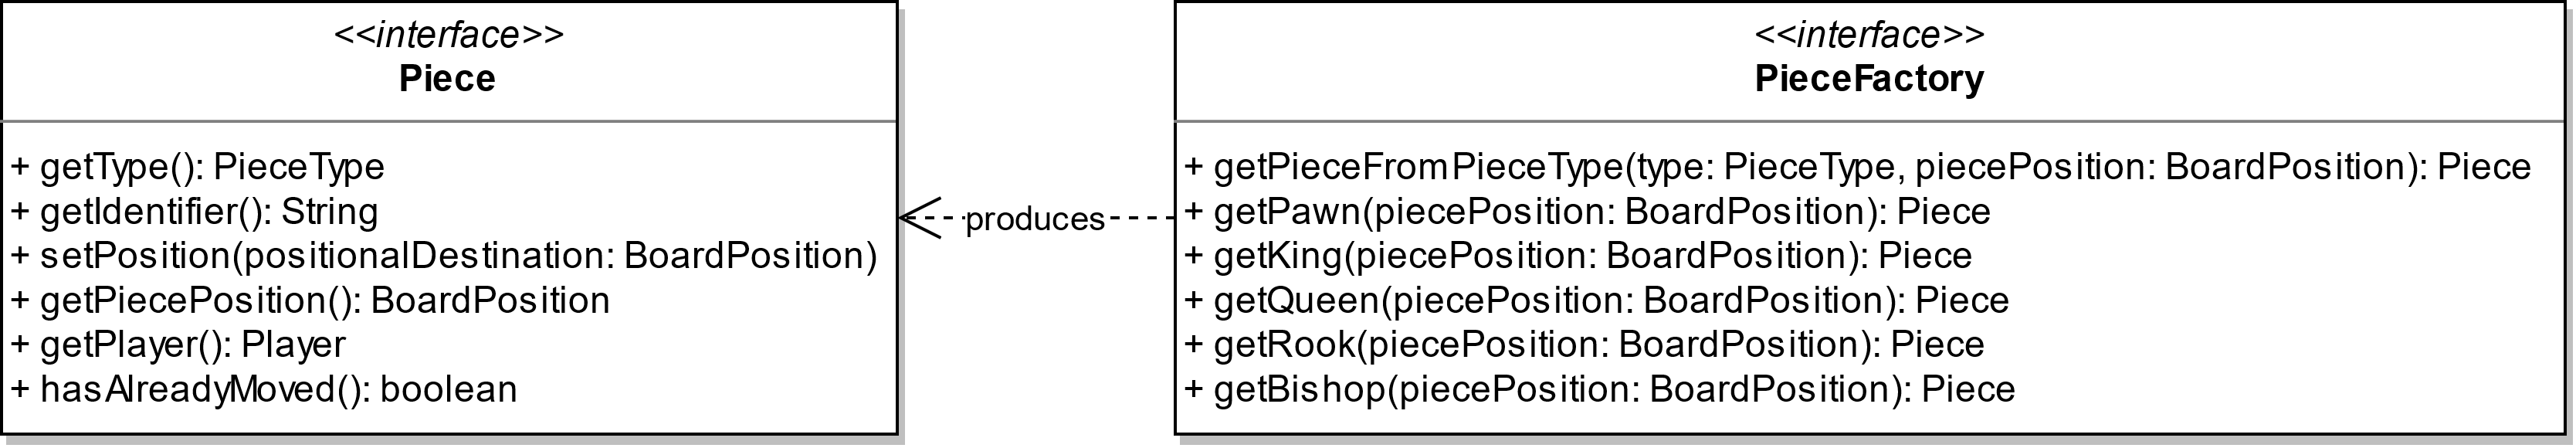
\includegraphics[width=\textwidth]{img/Stefano/Piece.png}
    \end{center}
    \caption{Struttura dell'entità \texttt{Piece} e sua rispettiva Factory}
    \label{img:Piece}
\end{figure}
\
\\
%
Ho invece deciso di utilizzare il pattern \textbf{Strategy}  per la realizzazione delle \texttt{MovementStrategy} dei vari pezzi. 
%
\\
\texttt{MovementStrategy} risulta essere una Functional Interface, avente come unico metodo \texttt{getPossibleMoves(...)}, che prende come argomento la \texttt{Board} attuale, e ritorna l'insieme delle possibili destinazioni.
% 
\\
Da notare che la \texttt{MovementStrategy} è in grado di fornire una strategia di movimento generale, statica rispetto ai concetti ed alle regole di gioco. Gli unici controlli "dinamici" apportati sono che un pezzo non può scavalcare/catturare un pezzo alleato oppure superare un pezzo nemico lungo la traiettoria definita da uno \texttt{UnaryOperator} sulle \texttt{BoardPosition}. Concetti e regole più specifiche sono gestiti, come detto precedentemente, in parte dal \texttt{MovementManager} ed in parte dal \texttt{GameController}.

\begin{figure}[H]
    \begin{center}
        \centering
        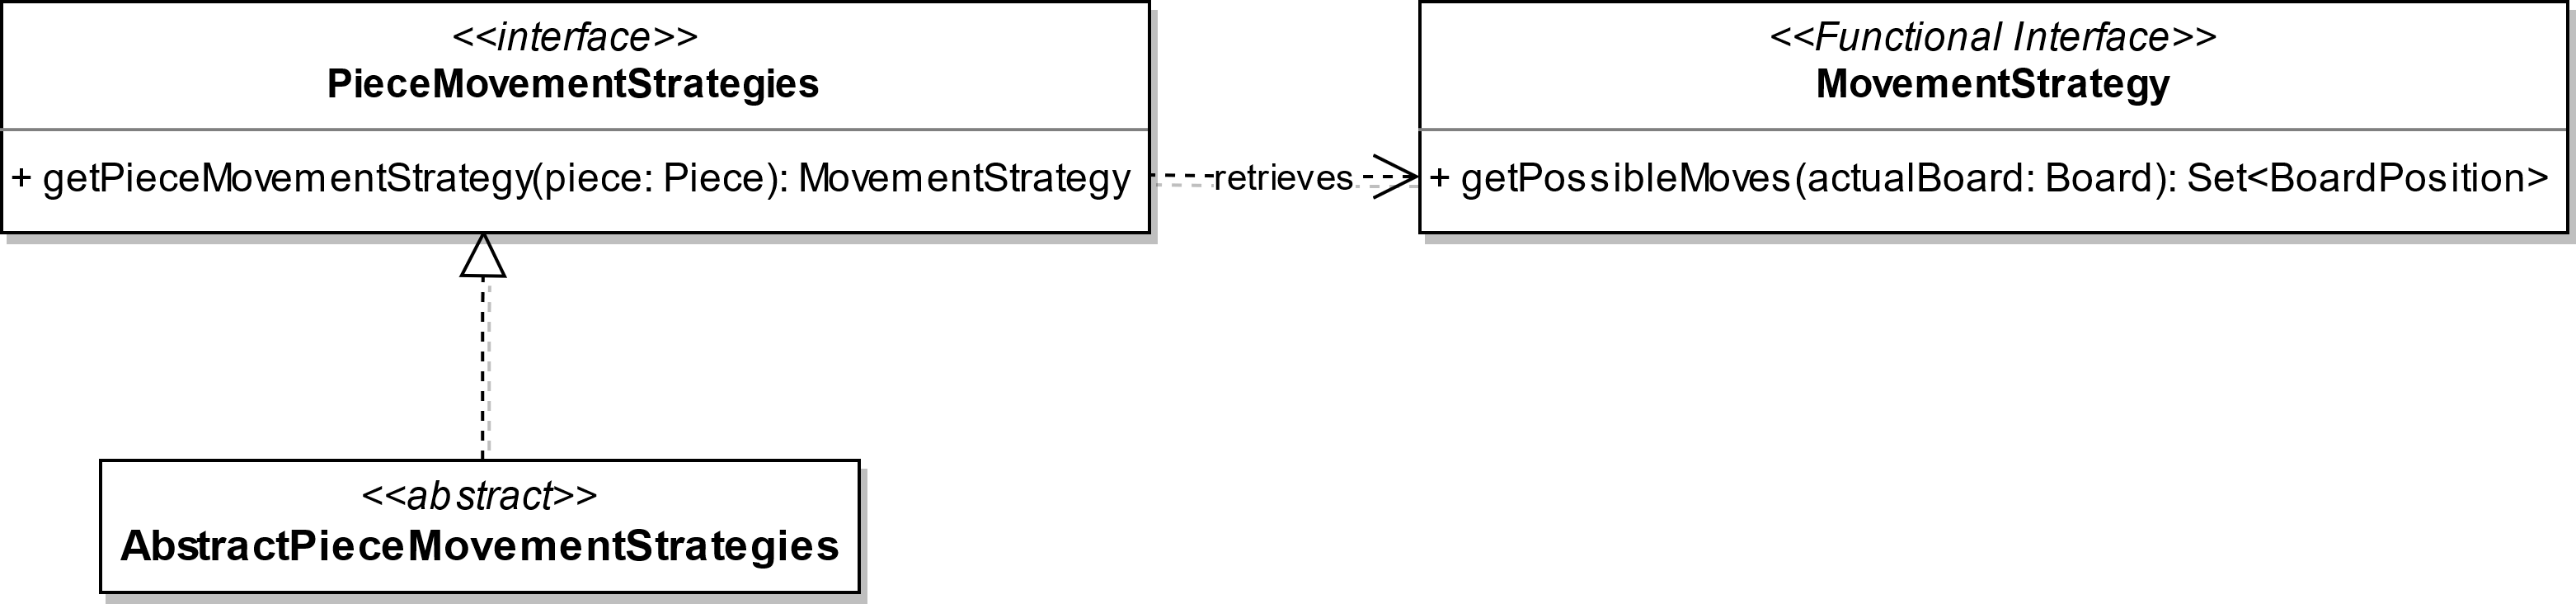
\includegraphics[scale=0.8]{img/Stefano/PieceMovementStrategies.png}
    \end{center}
    \caption{Struttura della \texttt{PieceMovementStrategies}}
    \label{img:PieceMovementStrategies}
\end{figure}
\
\\
%
Il calcolo della strategia di movimento di un \texttt{Piece} viene eseguito a run-time, l'unico modo per interfacciarsi dall'esterno con la \texttt{PieceMovementStrategies} risulta essere il metodo \texttt{getPieceMovementStrategy(...)}, che prendendo un pezzo in input è in grado di restituirne la corretta strategia di movimento, sulla quale andrà eventualmente invocato il metodo dell' interfaccia funzionale per conoscere le effettive destinazioni possibili secondo quella specifica strategia.
% 
\\
Per permetterne il funzionamento ho utilizzato in \texttt{AbstractPieceMovementStrategies} un \textbf{Template Method}, che è proprio \texttt{getPieceMovementStrategy(...)}. Quest' ultimo, in base al \texttt{PieceType}, deve scegliere quale metodo specifico invocare per calcolarne la corretta Strategy di movimento. Queste singole strategie di movimento dei singoli pezzi non sono univoche, ma variano a seconda della modalità di gioco. Sono infatti definite inizialmente da metodi abstract in \texttt{AbstractPieceMovementStrategies} e per questo ho dovuto ricorrere al Template Method sopracitato. 
\\
Ho inoltre deciso di utilizzare questa classe astratta in modo tale da racchiudere in essa le caratteristiche comuni a tutte le varianti, come lo è il metodo \texttt{getDestinationsFromFunction(...)}, responsabile della generazione di tutte le mosse possibili a partire da alcuni parametri in ingresso.

\begin{figure}[H]
\centering{}
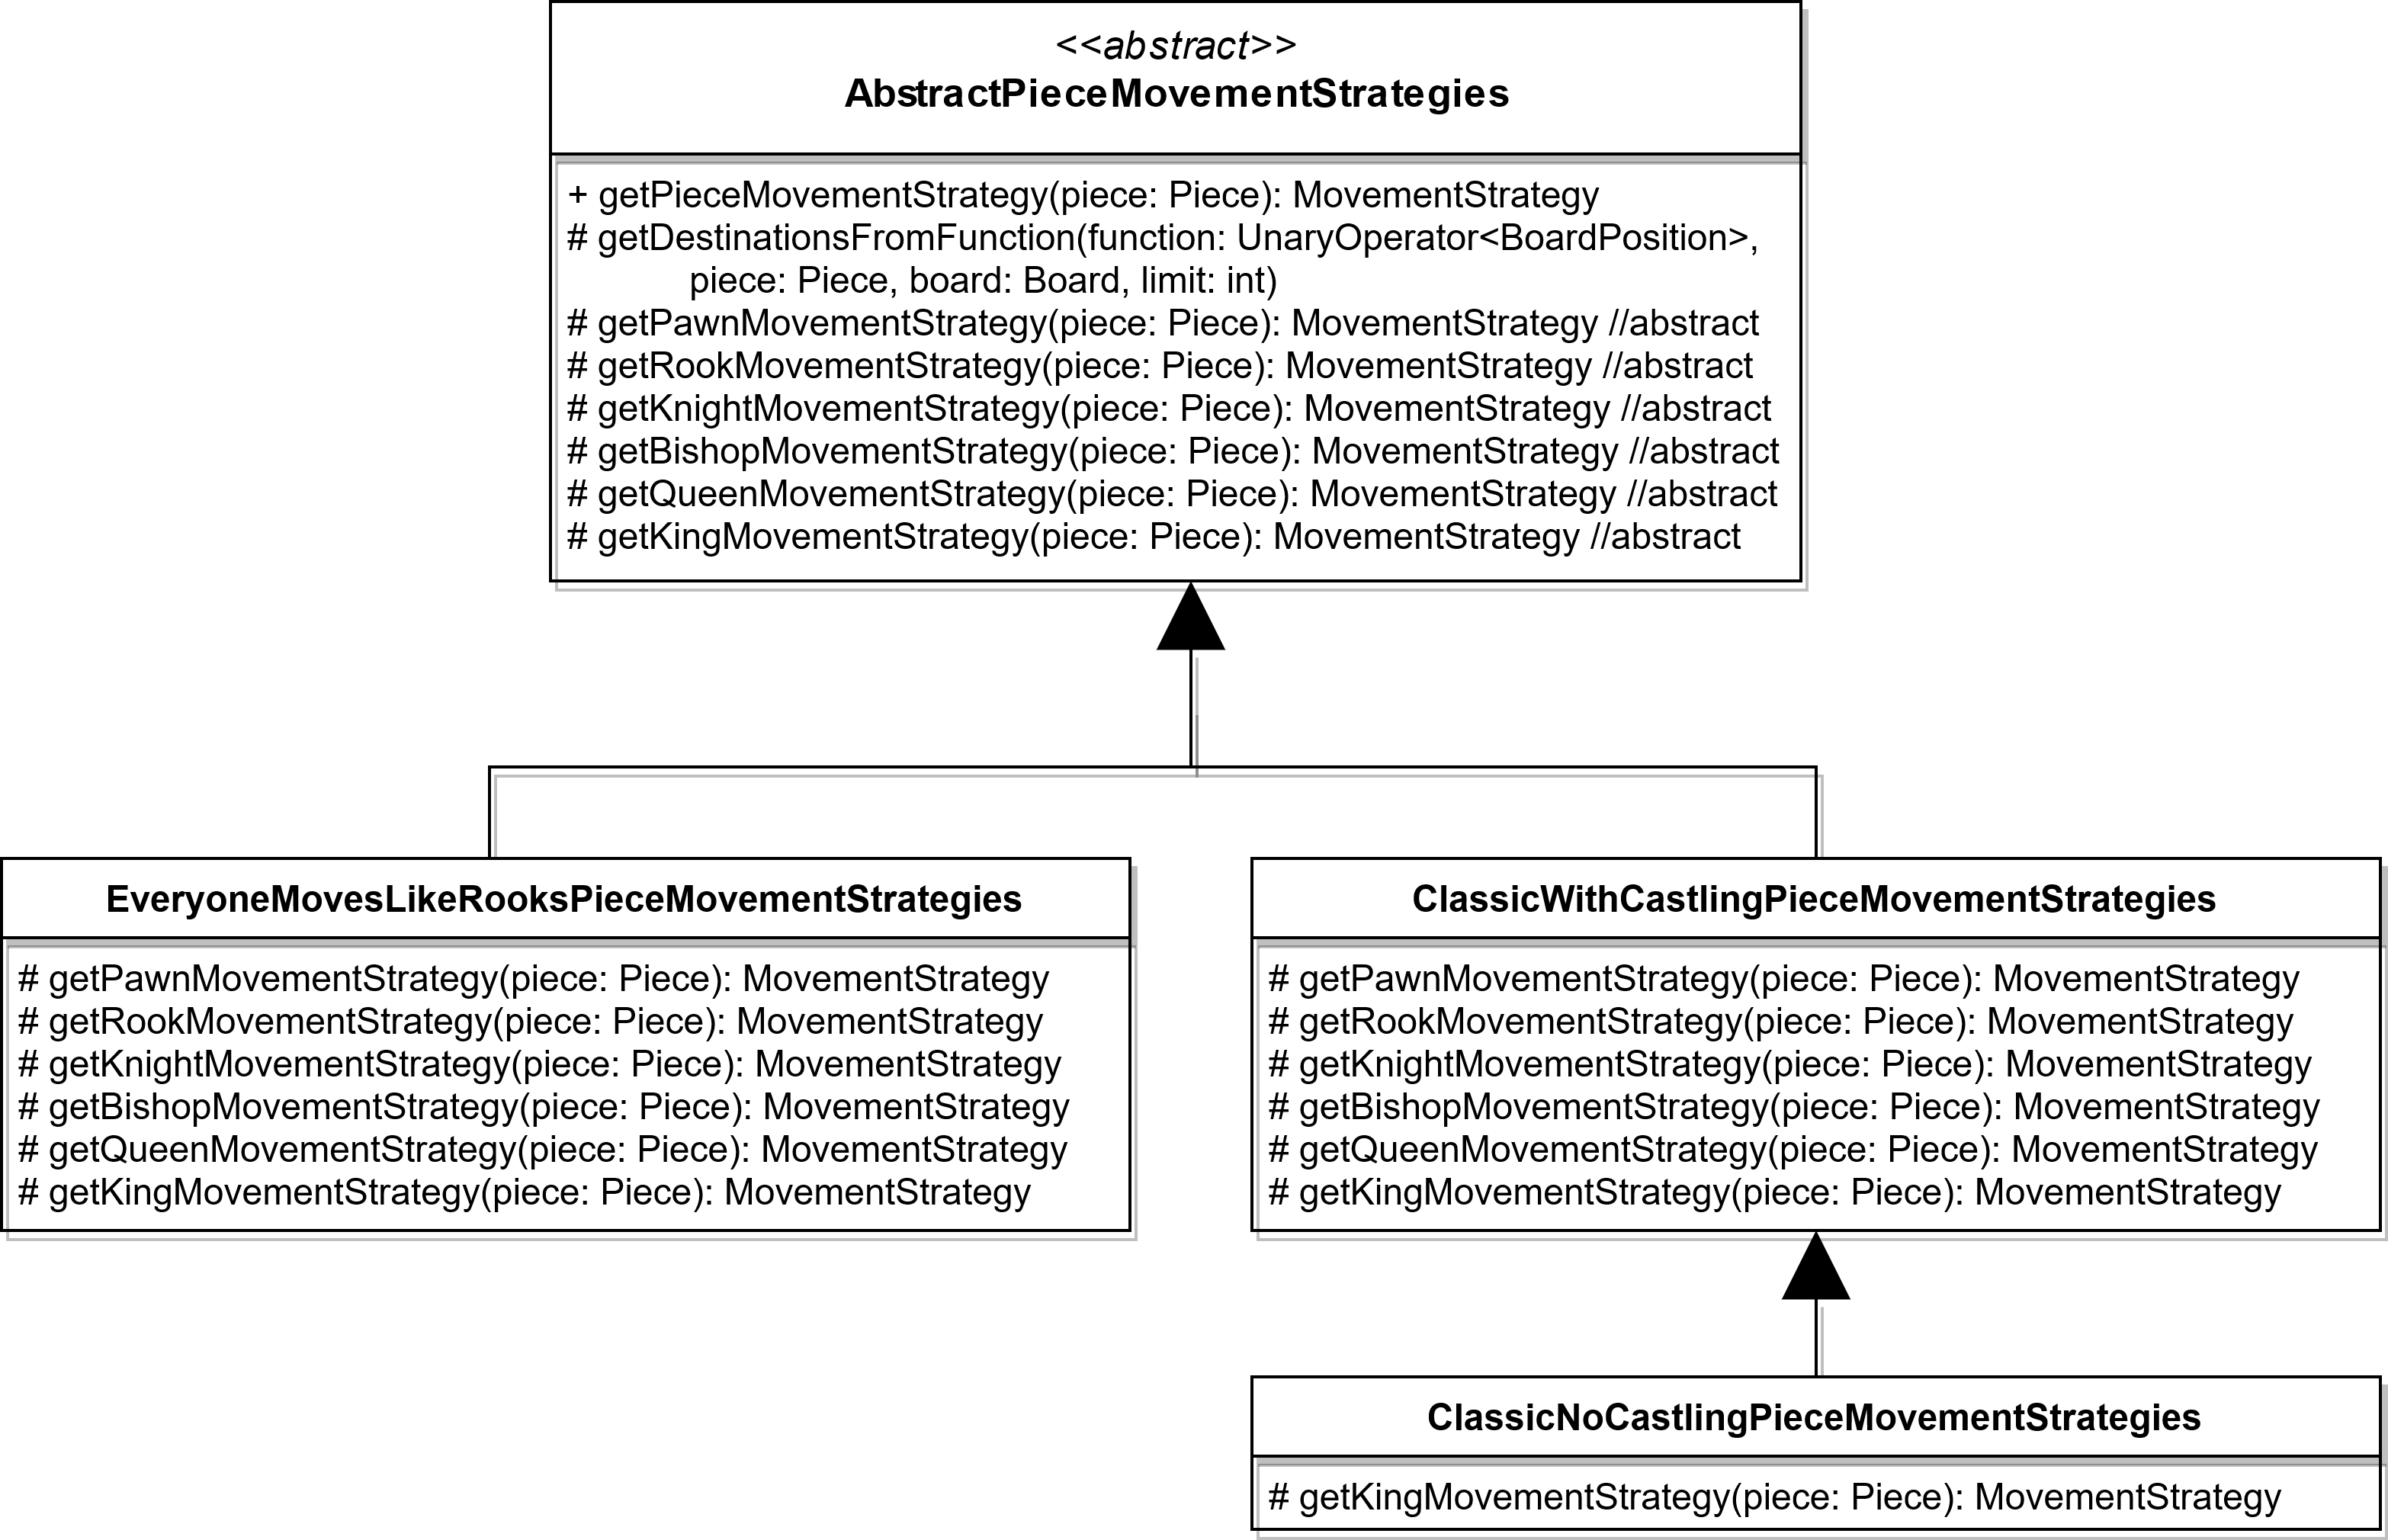
\includegraphics[width=\textwidth]{img/Stefano/TemplateMethodPieceMovementStrategies}
\caption{Interfacciamento con le strategie di movimento dei pezzi attraverso il Template Method \texttt{getPieceMovementStrategy()}}
\label{img:TemplateMethodPieceMovementStrategies}
\end{figure}
%
\
\\
Aggiungere nuove varianti risulta semplice e veloce. La modalità classica degli scacchi rifà le sue strategie di movimento alla \texttt{ClassicWithCastlingPieceMovementStrategies}.
Per alcune varianti risulta comodo estendere quest'ultima, andando poi a fare l'Override di solo quelle specifiche strategie di movimento dei pezzi che si vogliono modificare, lasciando invariate le altre. 

\begin{figure}[H]
\centering{}
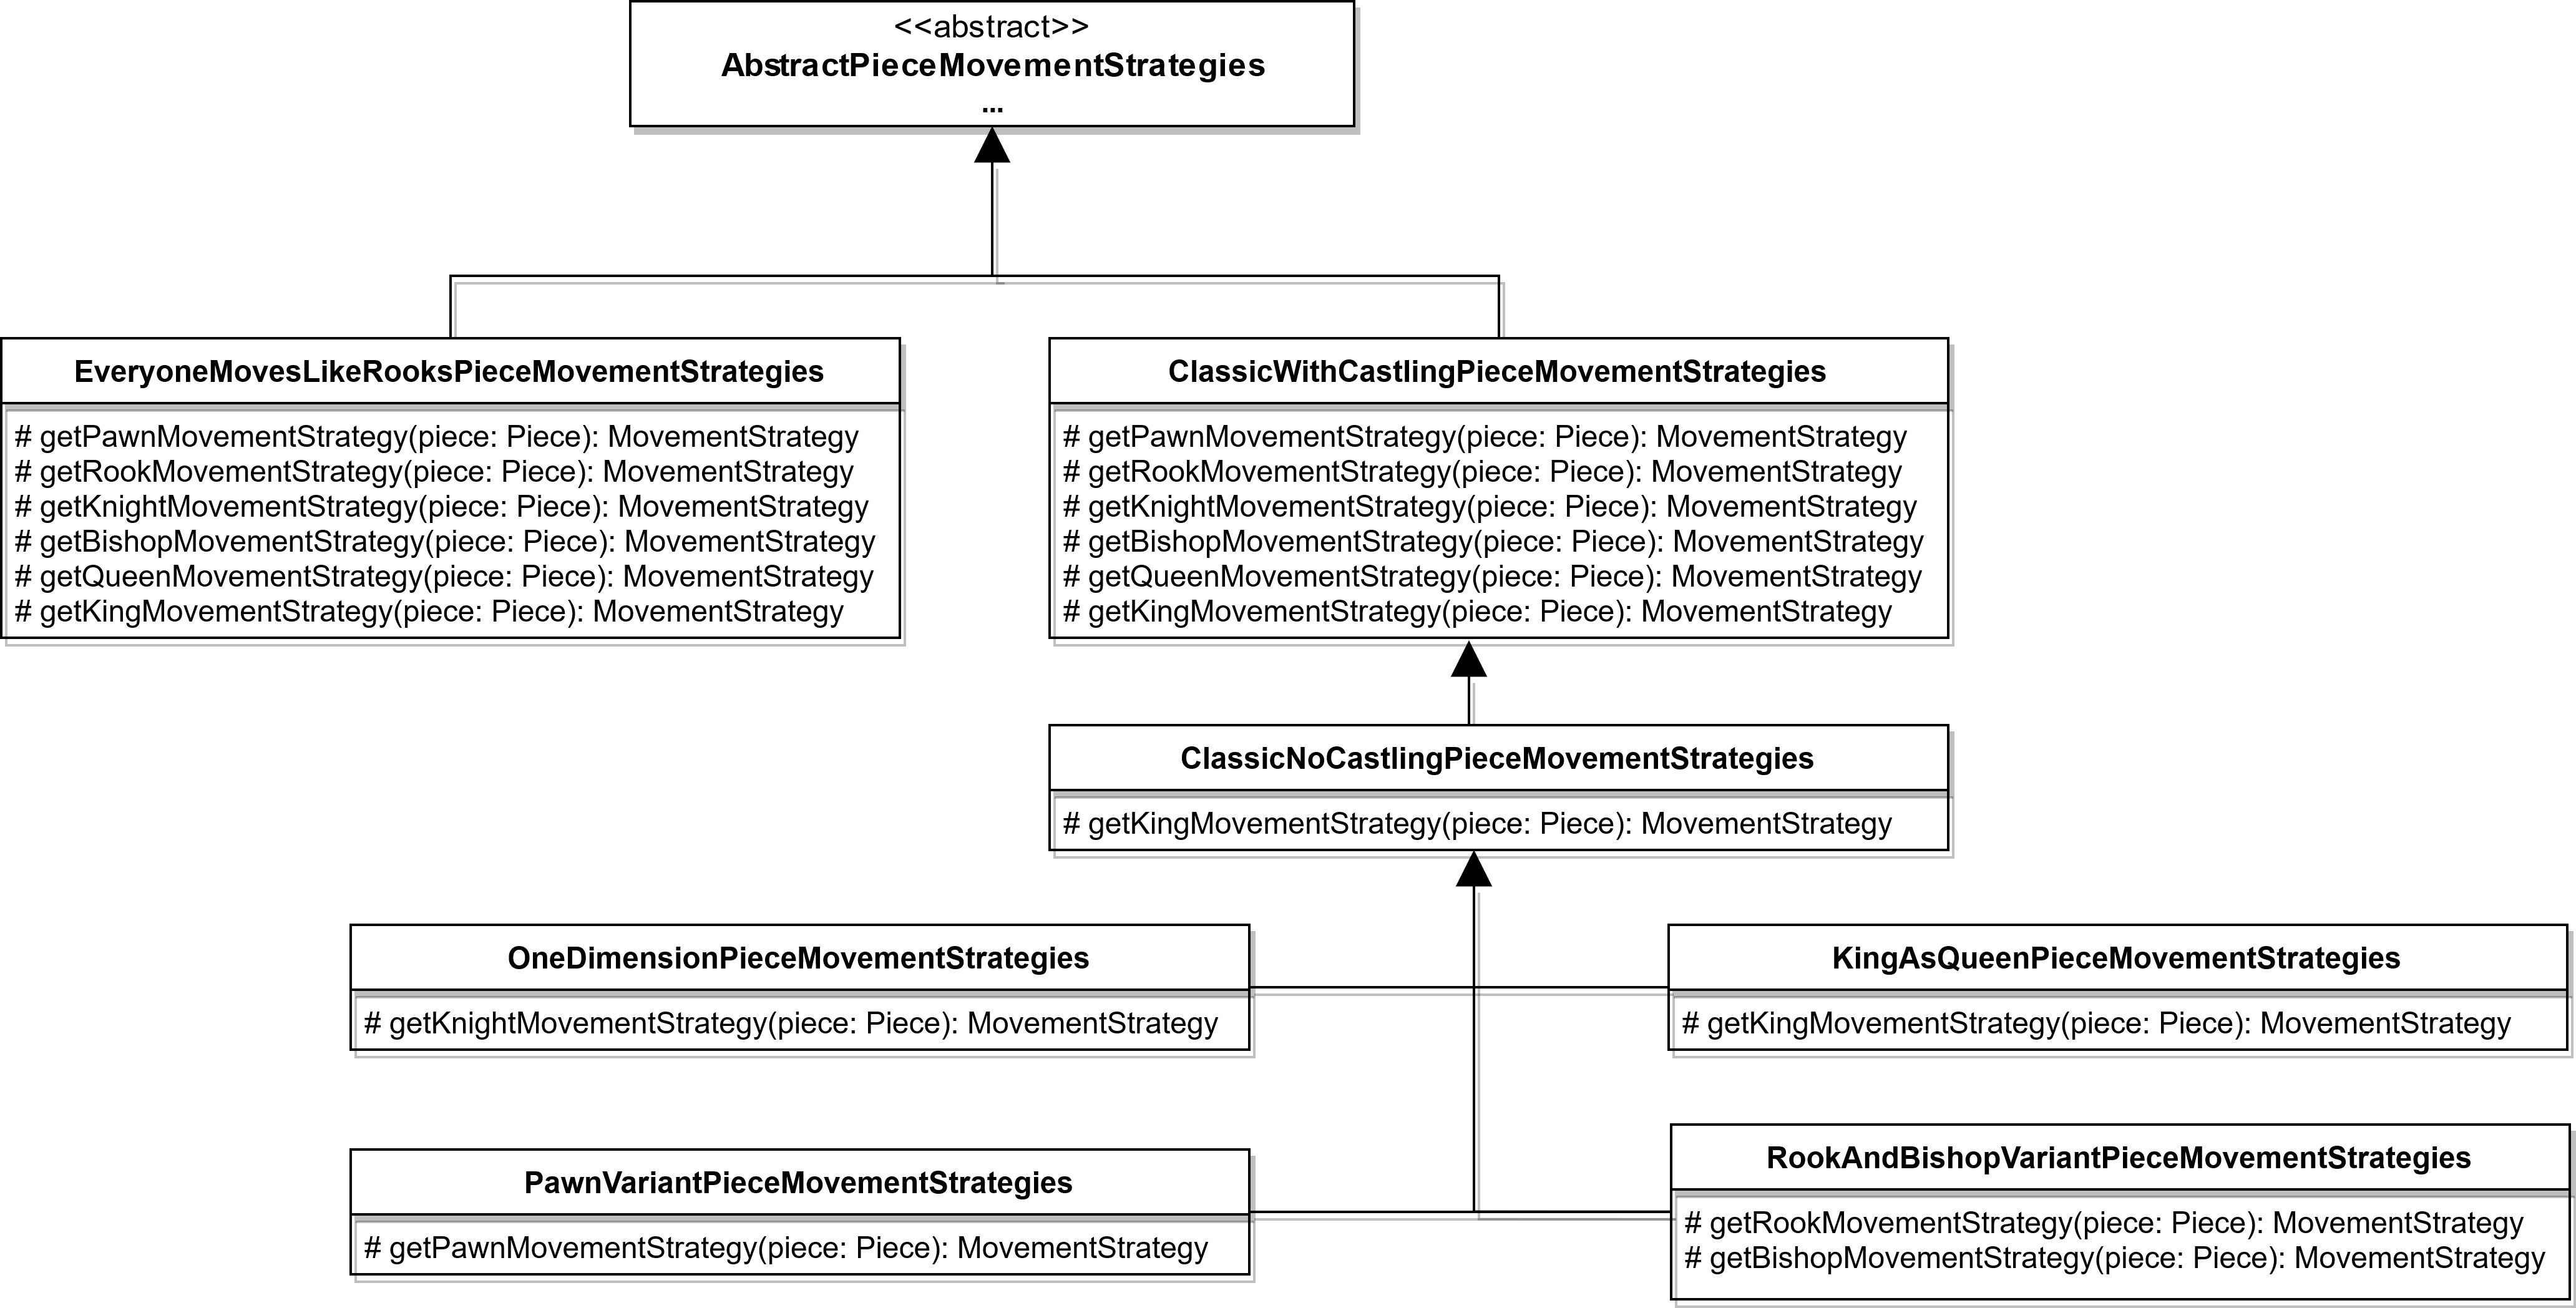
\includegraphics[width=\textwidth]{img/Stefano/PieceMovementStrategiesFocus.png}
\caption{Implementazione delle diverse \texttt{PieceMovementStrategies}}
\label{img:PieceMovementStrategiesFocus}
\end{figure}
\
\\
%
Per altre invece, per le quali si intende modificare completamente tutte le strategie di movimento di tutti i pezzi, discostandole da quello che è la modalità classica, conviene invece estendere direttamente da \texttt{AbstractPieceMovementStrategies}.\\
\texttt{EveryoneMovesLikeRooksPieceMovementStrategies} ne è un esempio.
\\
Essendo poi riuscito a catturare il modo attraverso cui sono individuate le possibili destinazioni per le varie \texttt{MovementStrategy} con \texttt{getDestinationsFromFunction(...)}, la generazione di queste risulta anche molto snella.

\subsubsection{Game Controller}

Il \texttt{GameController}, come prima visto, è utilizzato soprattutto all'interno della \texttt{MovementManager}.
\\
Ruolo del \texttt{GameController} è quello di implementare quelle che sono le regole della partita di scacchi, gestendo quindi i concetti di scacco, scacco matto, stallo e vittoria.
\\
\texttt{MovementManager}, \texttt{PieceMovementStrategies} assieme al \texttt{GameController} possono essere considerate come la triade rappresentante il cuore del motore di gioco.
\\
Il \texttt{GameController} è utilizzato quindi per conoscere lo stato attuale della partita dal punto di vista delle regole scacchistiche, appunto per questo è fondamentale all' interno del \texttt{MovementManager}.
\\
Poichè il \texttt{GameController} è colui che analizza lo stato della partita è l'unico in grado di sapere se effettuare una mossa causerà uno scacco o meno. Questo controllo è eseguito con il metodo \texttt{wouldNotBeInCheck(...)}, che preso un \texttt{PieceMovement}, è in grado di valutare se porterà o meno ad uno stato di scacco, portando a considerare quindi quest' ultima una mossa illegale(oppure no, in base alla variante).

\begin{figure}[H]
    \begin{center}
        \centering
        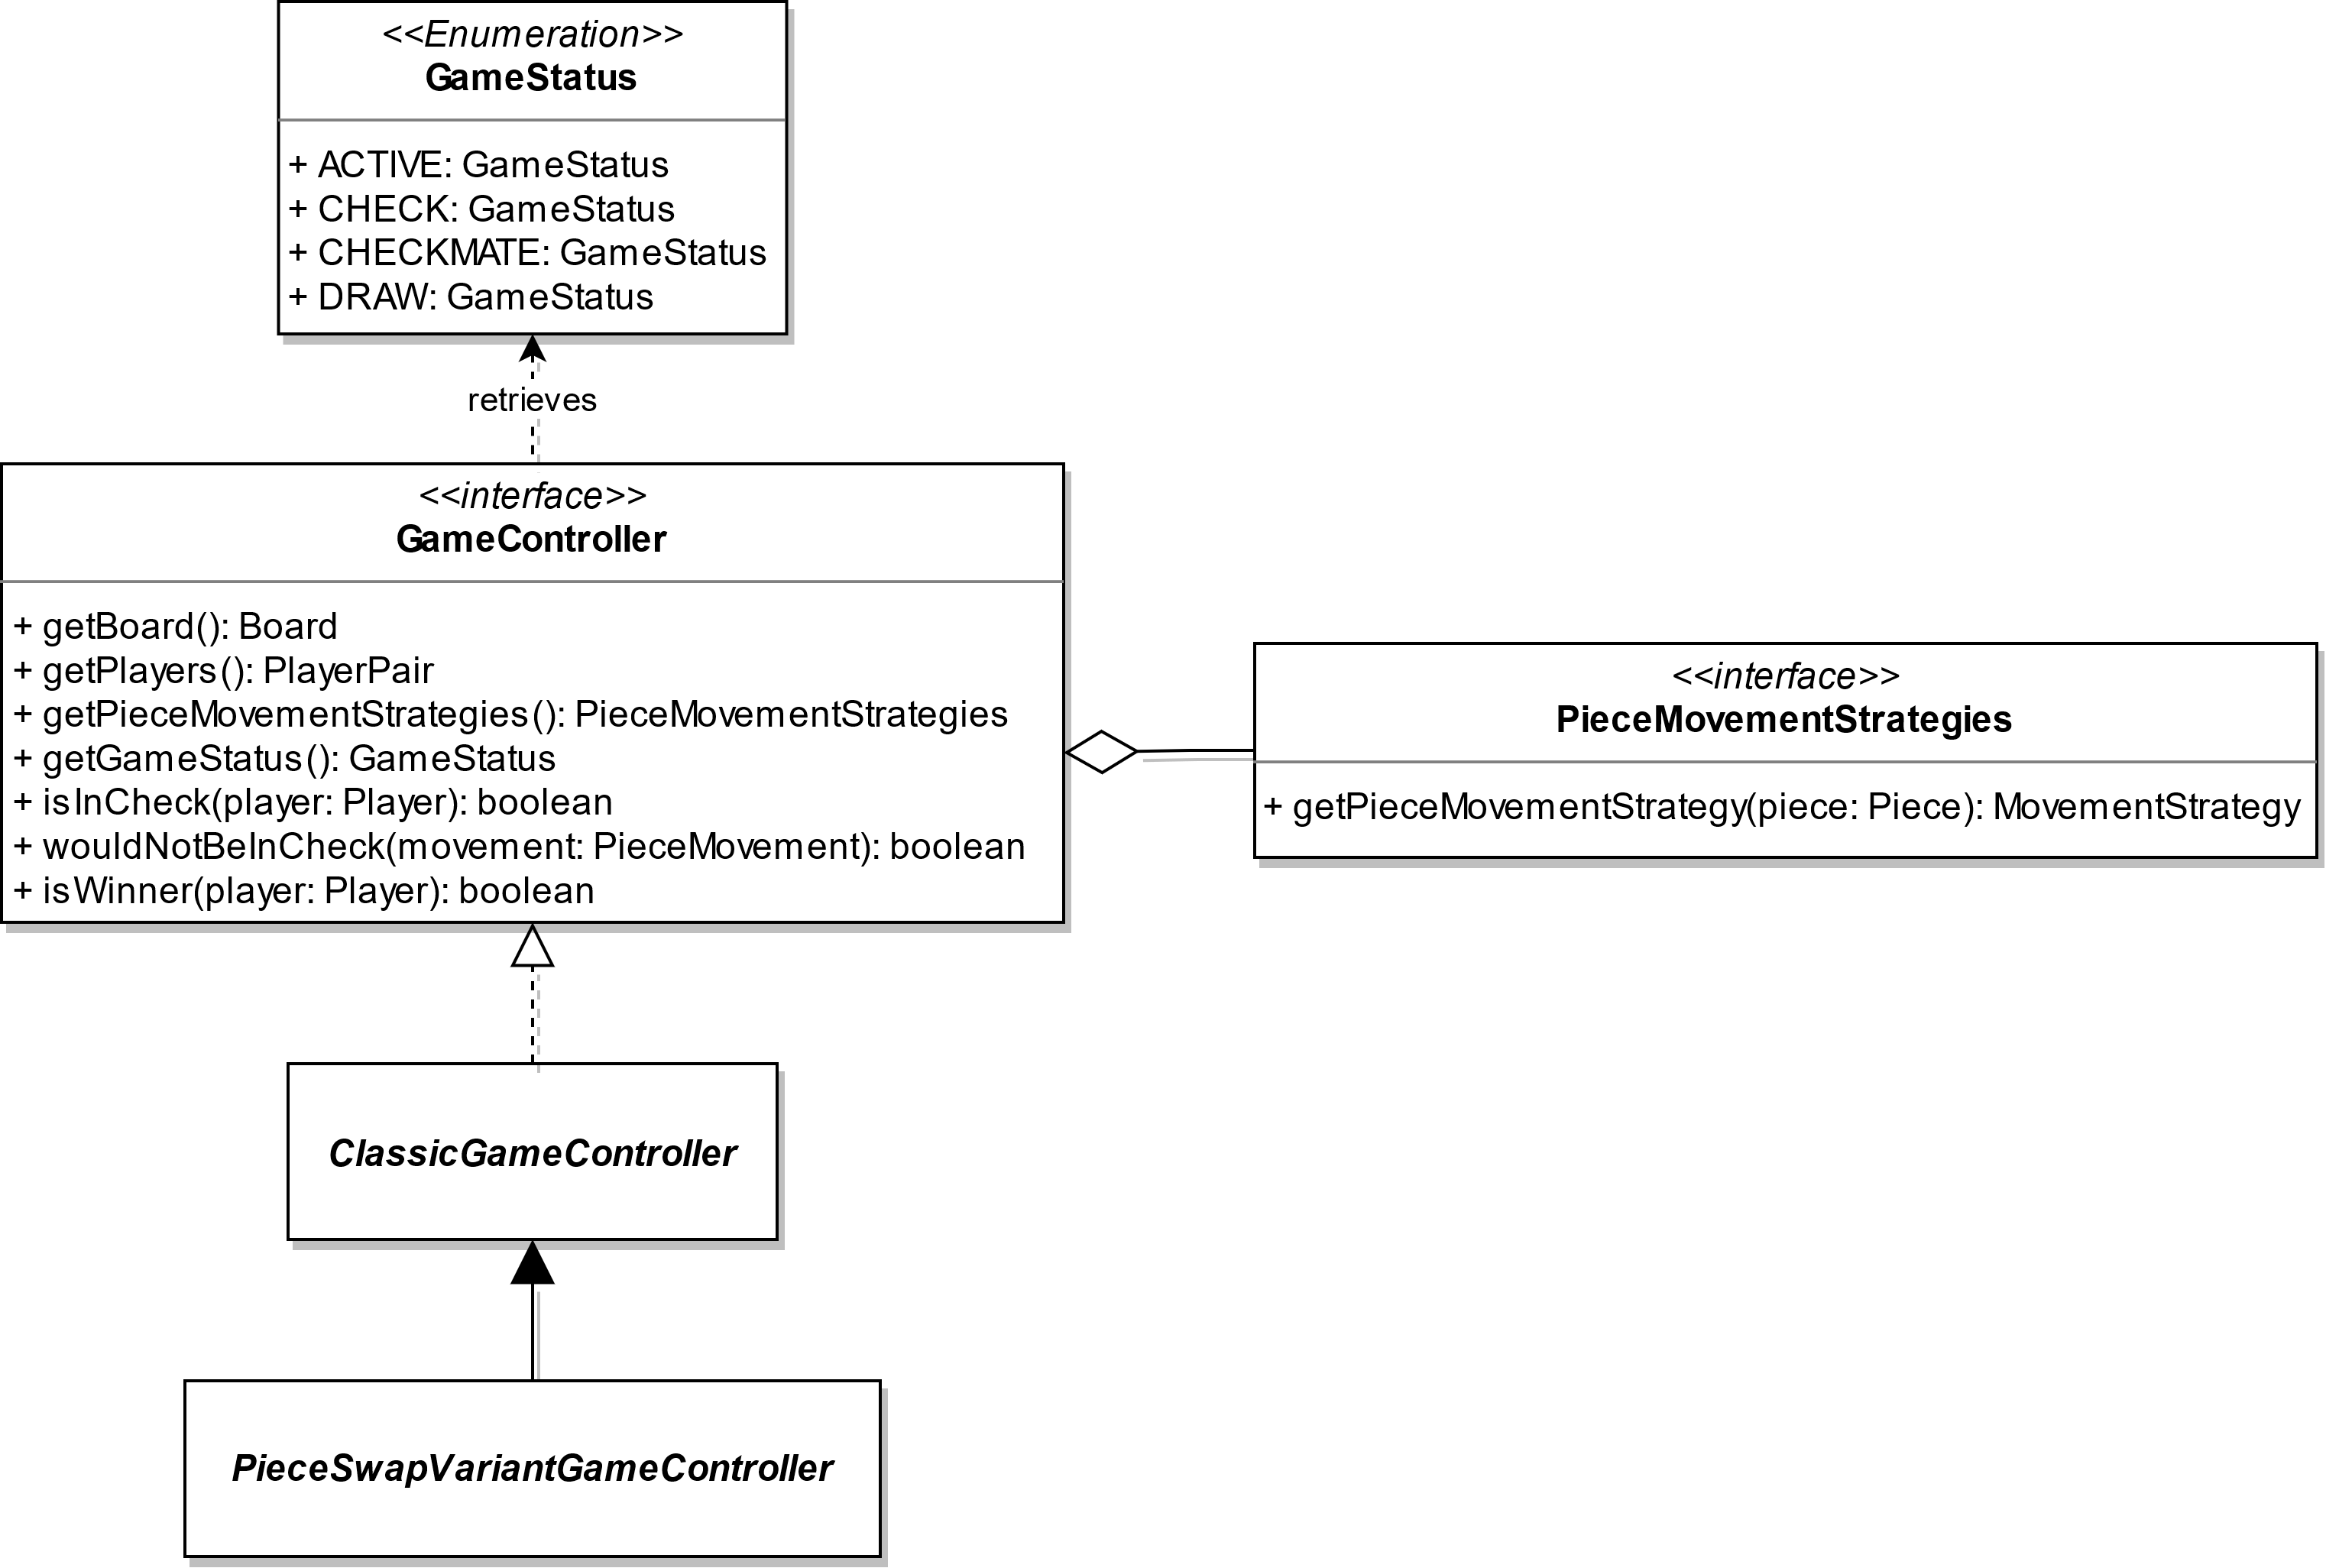
\includegraphics[scale=0.8]{img/Stefano/GameController.png}
    \end{center}
    \caption{Struttura del GameController}
    \label{img:GameController}
\end{figure}
\
\\
Il \texttt{MovementManager} utilizza ampiamente questo metodo quando deve valutare se la mossa eseguita dall'utente sia o meno valida.
Inoltre, il \texttt{GameController} fa ampio uso della \texttt{PieceMovementStrategies} per sapere come si possano muovere i pezzi sulla scacchiera, in modo tale da poter trovare eventuali mosse in grado di salvare un giocatore da una potenziale situazione di scacco matto.
\\
Quasi tutte le modalità di gioco utilizzano la \texttt{ClassicGameController}, che esprime quelle che sono le regole della modalità classica degli scacchi. Unica eccezione è la variante \texttt{PieceSwapVariantGameController}, per la quale è stato necessario ridefinire la condizione di \href{https://support.chess.com/article/128-what-does-insufficient-mating-material-mean}{\underline{patta legata a "materiale insufficiente"}}.

\subsubsection*{MovementManager}
Per poter facilmente conoscere la fattibilità o meno di una mossa eseguita, è stata necessaria la creazione di un \texttt{MovementManager}, il cui compito principale è quello di verificare la correttezza di una mossa e gestire i side-effect provocati dalla suddetta, comunicando poi il risultato/conseguenza che questa ha provocato.\\
Per la realizzazione del \texttt{MovementManager} ho deciso di utilizzare il pattern \textbf{Facade}. Infatti, nonostante vi sia necessità di interagire con diversi oggetti, eseguendo altrettanti controlli per determinare la fattibilità della mossa passata, interagire con il \texttt{MovementManager} non risulta complesso, bensì "straightforward".
\\
L'architettura definita può essere infatti vista come "layered": il \texttt{GameController} è utilizzato all'interno del \texttt{MovementManager}, e la \texttt{PieceMovementStrategies} all'interno del \texttt{GameController}. L'interfacciamento principale con "l'esterno" è il metodo \texttt{move(...)}.\\
Inoltre, per evitare di dare troppe responsabilità alla sola \texttt{MovementManager} ho scelto di comporre quest'ultima di una \texttt{MovementHandlerStrategy}, che si occupa delle sole verifiche riguardo la correttezza/fattibilità della mossa passata. Ho favorito quindi la composition, catturando funzionalità tra loro affini tramite oggetti.

\begin{figure}[H]
\centering{}
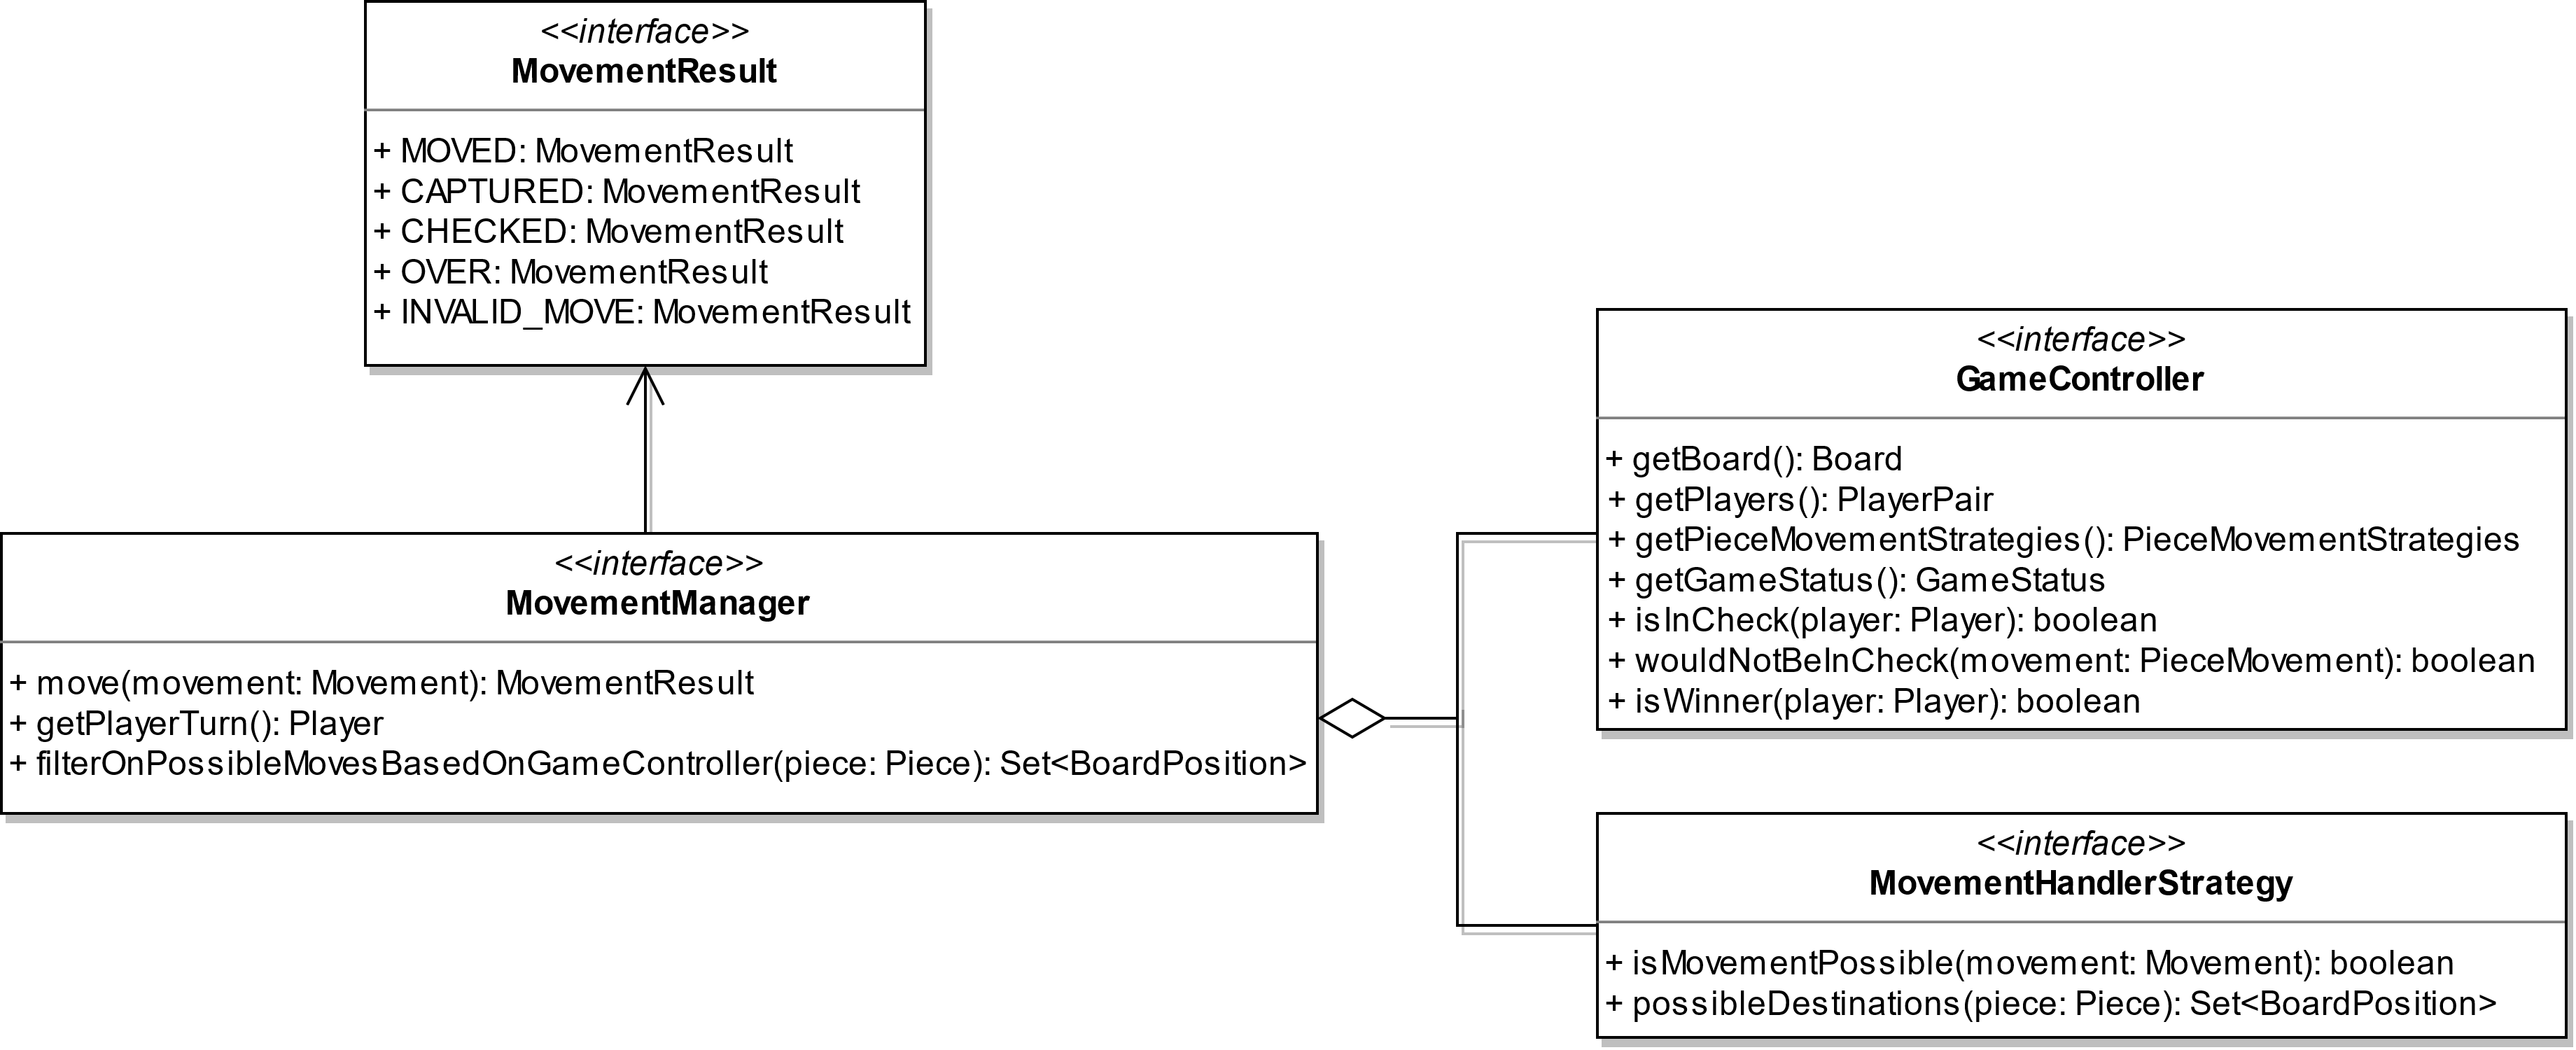
\includegraphics[width=\textwidth]{img/Stefano/CompleteMovementManager.png}
\caption{Gestione delle mosse attraverso il \texttt{MovementManager}}
\label{img:CompleteMovementManager}
\end{figure}
\
\\
%
Una mossa, detta \texttt{Movement}, contiene le sole informazioni essenziali, quali posizione di origine e di destinazione. Dalla \texttt{BasicMovement} estende la \texttt{PieceMovement}, che in più contiene anche il \texttt{Piece} interessato dalla mossa ed un metodo per eseguire la mossa stessa, andando a modificare con una \texttt{SetPosition} la posizione attuale del \texttt{Piece} da \texttt{Origin} a \texttt{Destination}.
\begin{figure}[H]
\centering{}
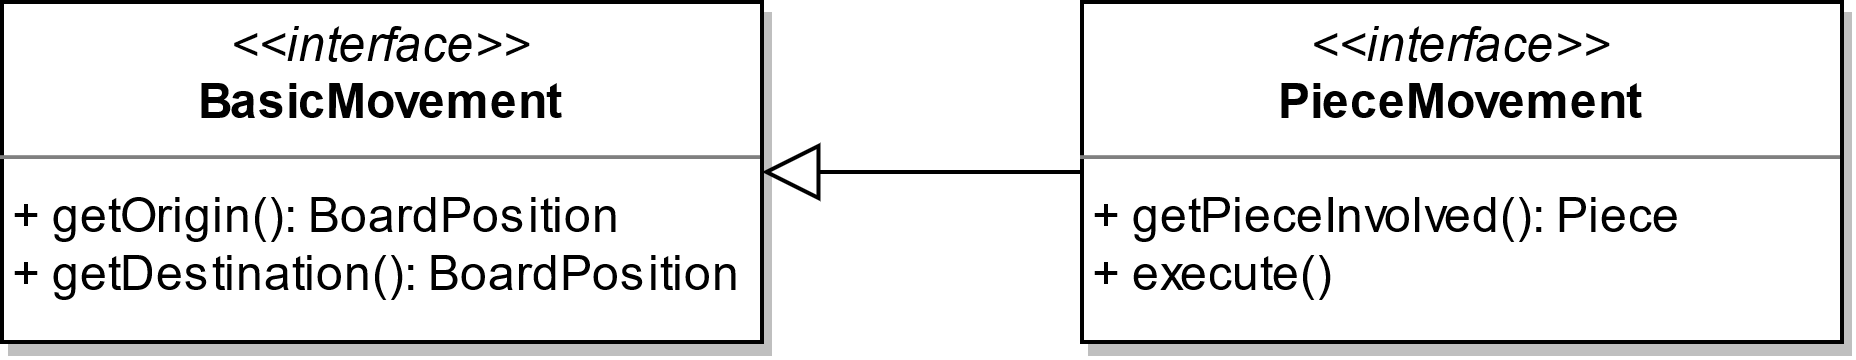
\includegraphics[scale=0.8]{img/Stefano/Movement.png}
\caption{Focus di dettaglio sui Movement}
\label{img:Movement}
\end{figure}
\
\\
%
Perchè il concetto di estendibilità non poteva fermarsi alle sole strategie di movimento, anche la maniera attraverso cui è gestita la fase di verifica e gestione delle conseguenze presenta una struttura facilmente estendibile e modificabile.\\
Con side-effect si intende, nel caso della modalità classica per esempio, la rimozione dei pezzi catturati, la promozione dei pedoni una volta raggiunta l'ottava traversa per i bianchi(oppure la prima per i neri) oppure lo spostamento della torre in caso di arrocco.

\begin{figure}[H]
\centering{}
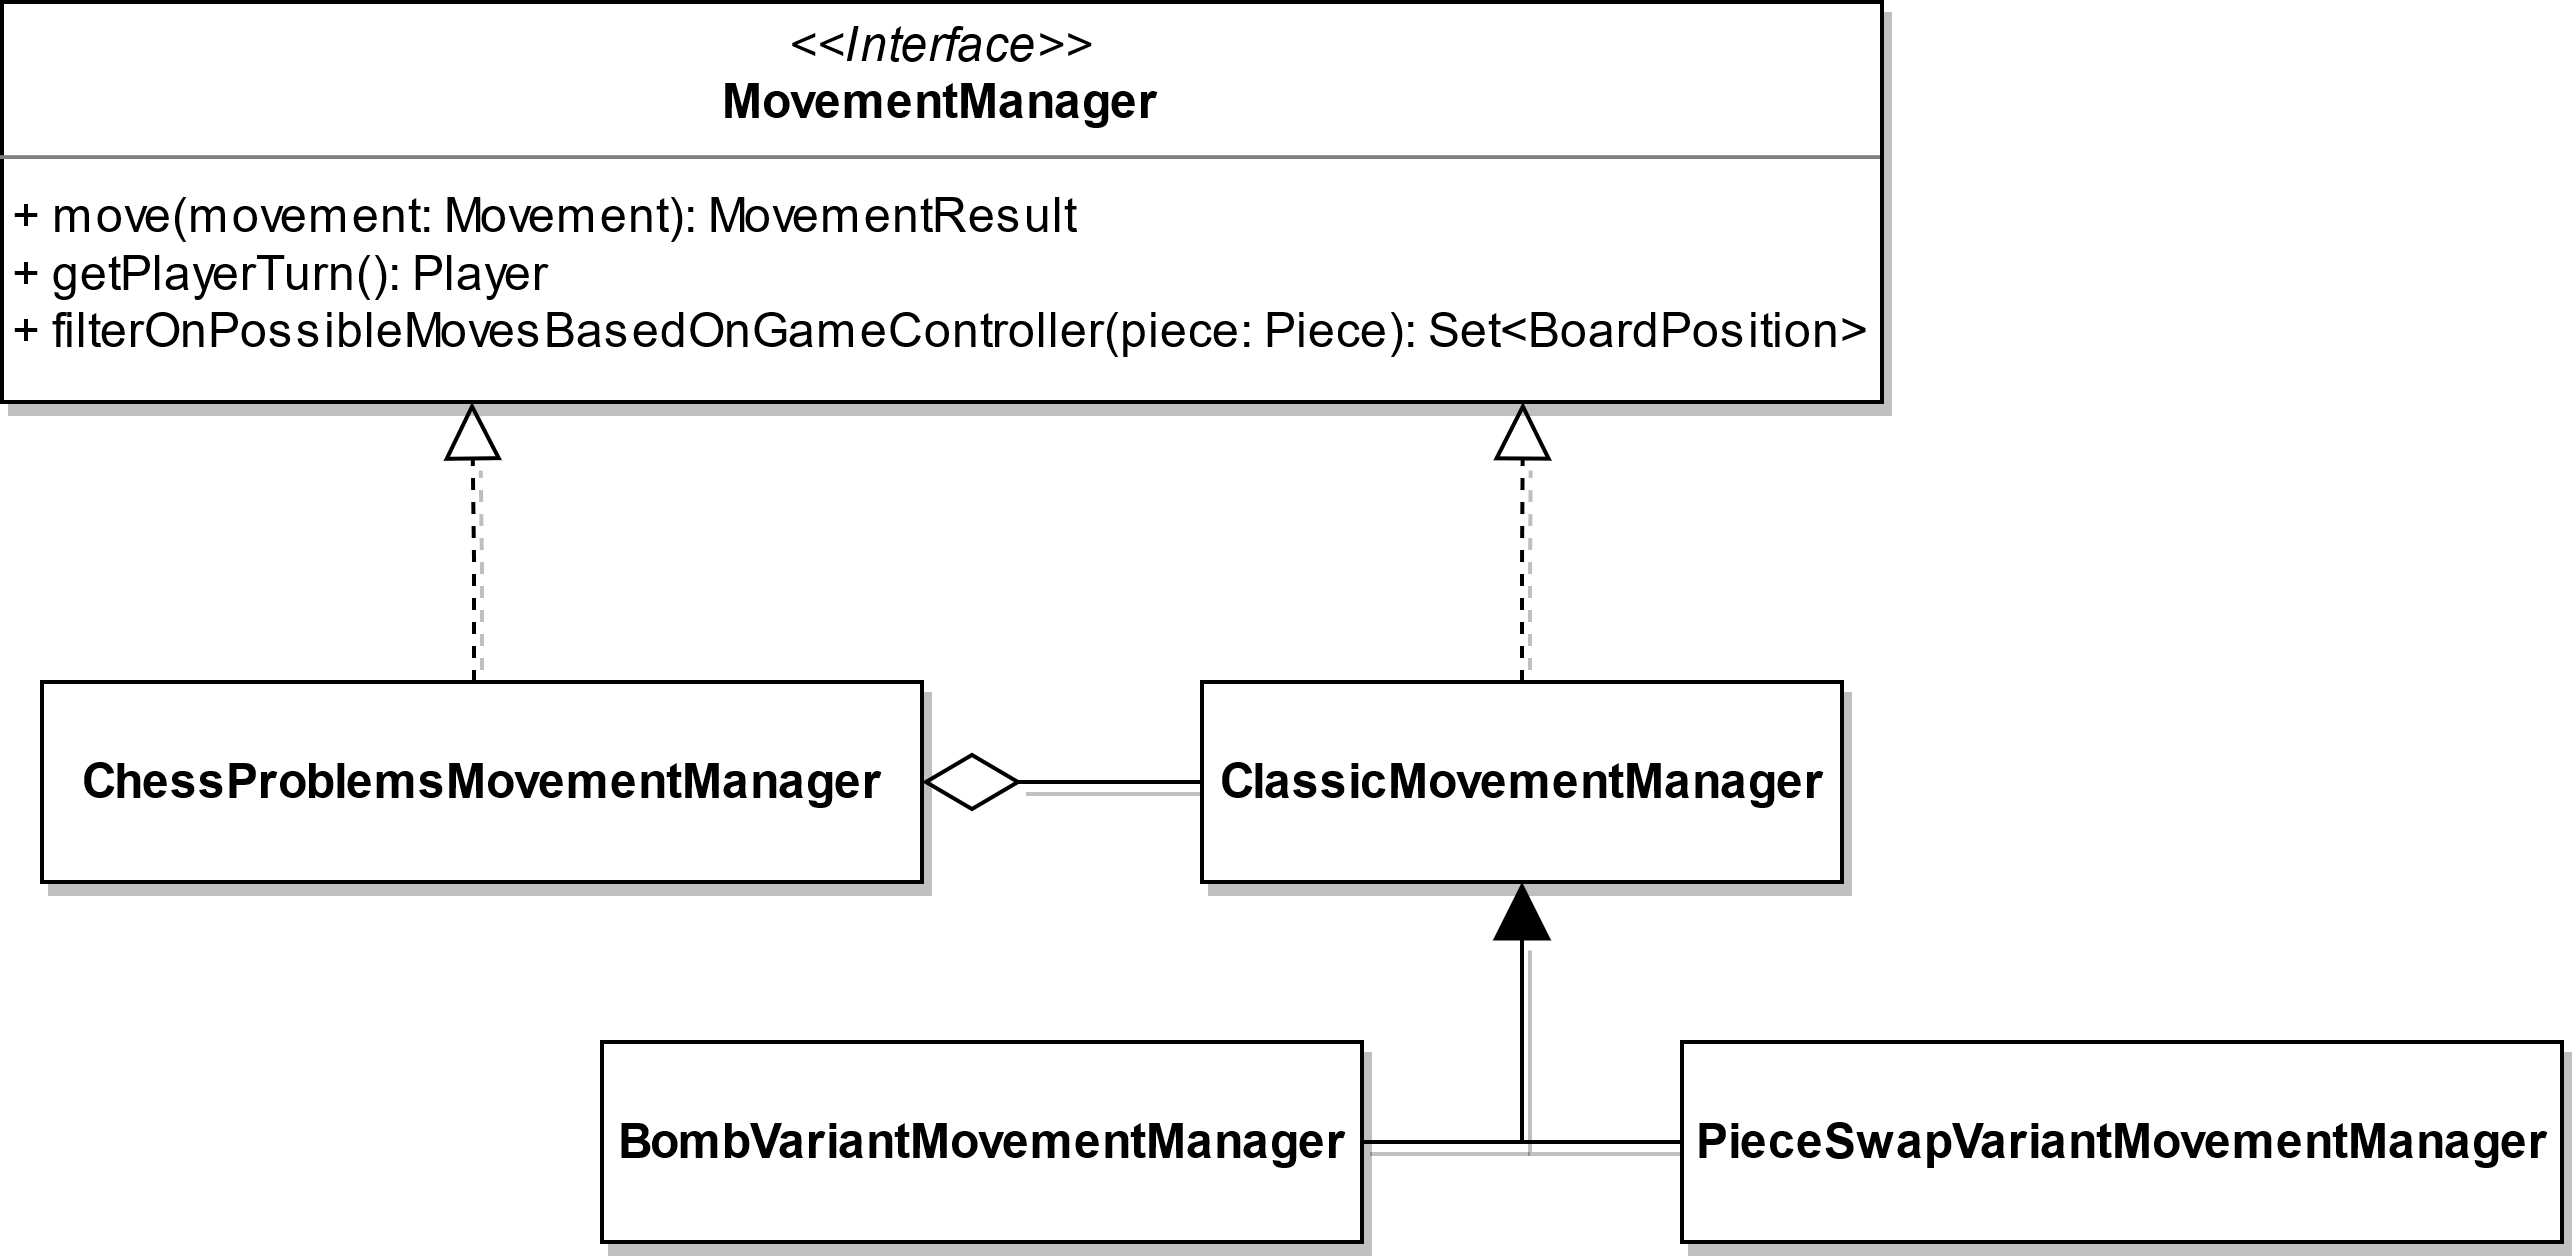
\includegraphics[scale=0.9]{img/Stefano/FocusMovementManager.png}
\caption{Implementazione dei vari \texttt{MovementManager}}
\label{img:FocusMovementManager}
\end{figure}
\
\\
Anche in questo caso è stato alquanto rapido e privo di difficoltà creare dei \texttt{MovementManager} alternativi a quello classico. Come la \texttt{PieceSwapMovementManager}, il cui side-effect particolare è quello di modificare secondo uno schema fisso il \texttt{PieceType} del pezzo appena mosso. Quando eseguita una mossa con una torre, questa si trasforma in un alfiere, quando mosso un alfiere, questo diventa un cavallo, e quest'ultimo quando mosso invece diventa una torre.\\
Oppure la \texttt{BombVariantMovementManager}, che come conseguenza ad una mossa ha la possibile "esplosione" del pezzo appena mosso, provocando la rimozione di tutti i pezzi che si trovino all'interno di un range randomico.
\
\\
Anche l'implementazione dei problemi scacchistici necessitava di un proprio \texttt{MovementManager}, ma perchè la modalità di gioco che interessava i problemi era proprio quella classica, ed un \texttt{MovementManager} di quel tipo esisteva già, ho scelto di utilizzare il pattern \textbf{Decorator}.
\texttt{ChessProblemsMovementManager} è un decorator del \texttt{ClassicMovementManager}. In più deve semplicemente verificare che la mossa effettuata sia quella corretta rispetto alla soluzione del problema scacchistico e come side-effect ulteriore deve eseguire la mossa dell'avversario una volta fatta quella corretta.
\\
Questa architettura permette di definire modularmente molte varianti scacchistiche per aggregazione delle diverse \texttt{PieceMovementStrategies}, \texttt{MovementManager} e \texttt{GameController} quando definito il \texttt{\nameref{Game}}.  


\subsubsection*{Chess Problems}

Un chess Problem è costituito da una \texttt{Board} iniziale, rappresentante la situazione in medias res che l'utente si trova a dover interpretare, e da una lista di mosse ordinate che rappresentano quelli che devono essere i \texttt{Movement} corretti per risolvere il problema.\\
I problemi sono affini alla modalità classica degli scacchi.\\
Per la loro creazione ho deciso di utilizzare il pattern \textbf{Factory}, questo mi ha permesso di generare molto semplicemente i vari problemi.
Necessitando questi di una \texttt{Board} di partenza, esattamente come tutte le altre modalità di gioco, ho deciso di creare anche una \texttt{StartingBoardFactory}, utilizzata sia dalle altre modalità di gioco, sia dai vari problemi scacchistici per reperire le diverse \texttt{Board} di partenza per le varie modalità.
\\
Per semplificare ulteriormente il compito alla \texttt{Factory} di \texttt{Board}, ho scelto di utilizzare il pattern \textbf{Builder} per la loro creazione.\\
Il manager dei movimenti per il problema scacchistico è stato descritto in precedenza. Proprio a quest' ultimo spetta il compito di verificare se la mossa effettuata dall' utente corrisponda ordinatamente a quella corretta secondo la lista definita dal problema.
\begin{figure}[H]
\centering{}
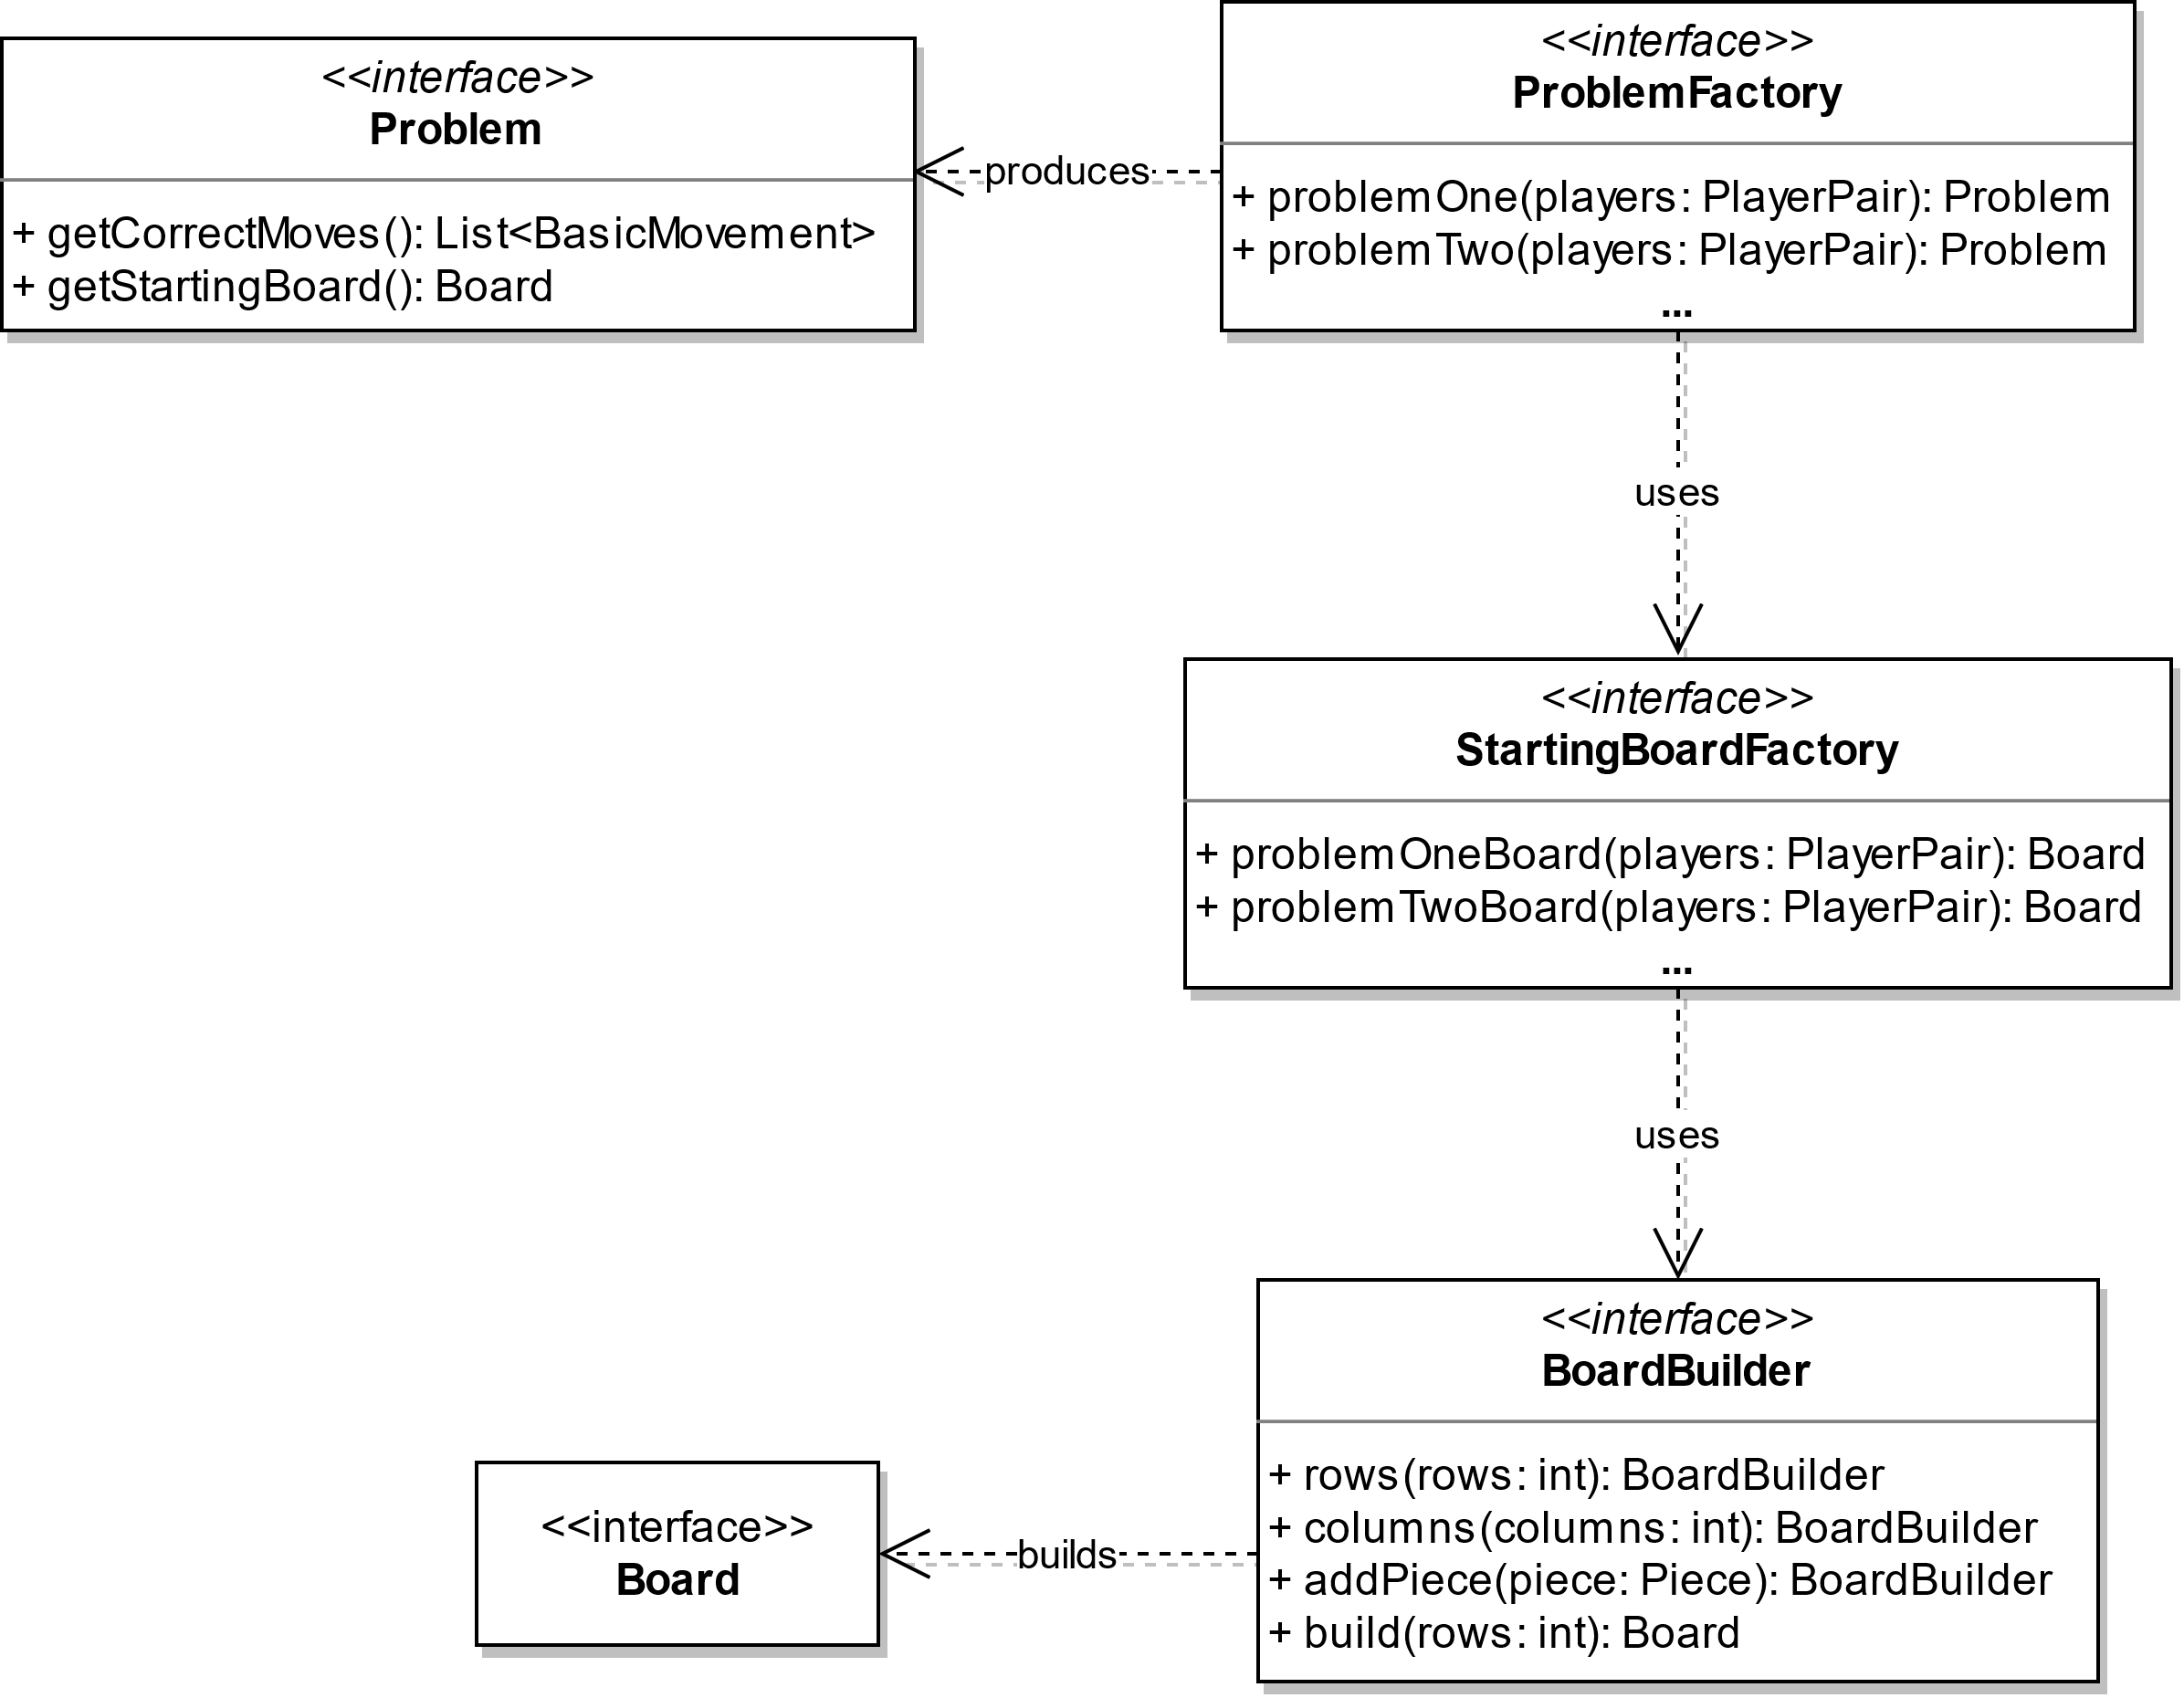
\includegraphics[scale=0.8]{img/Stefano/ChessProblem}
\caption{Gestione e creazione dei chess Problem}
\label{img:ChessProblem}
\end{figure}
\
\begin{figure}[H]
    \begin{center}
        \centering
        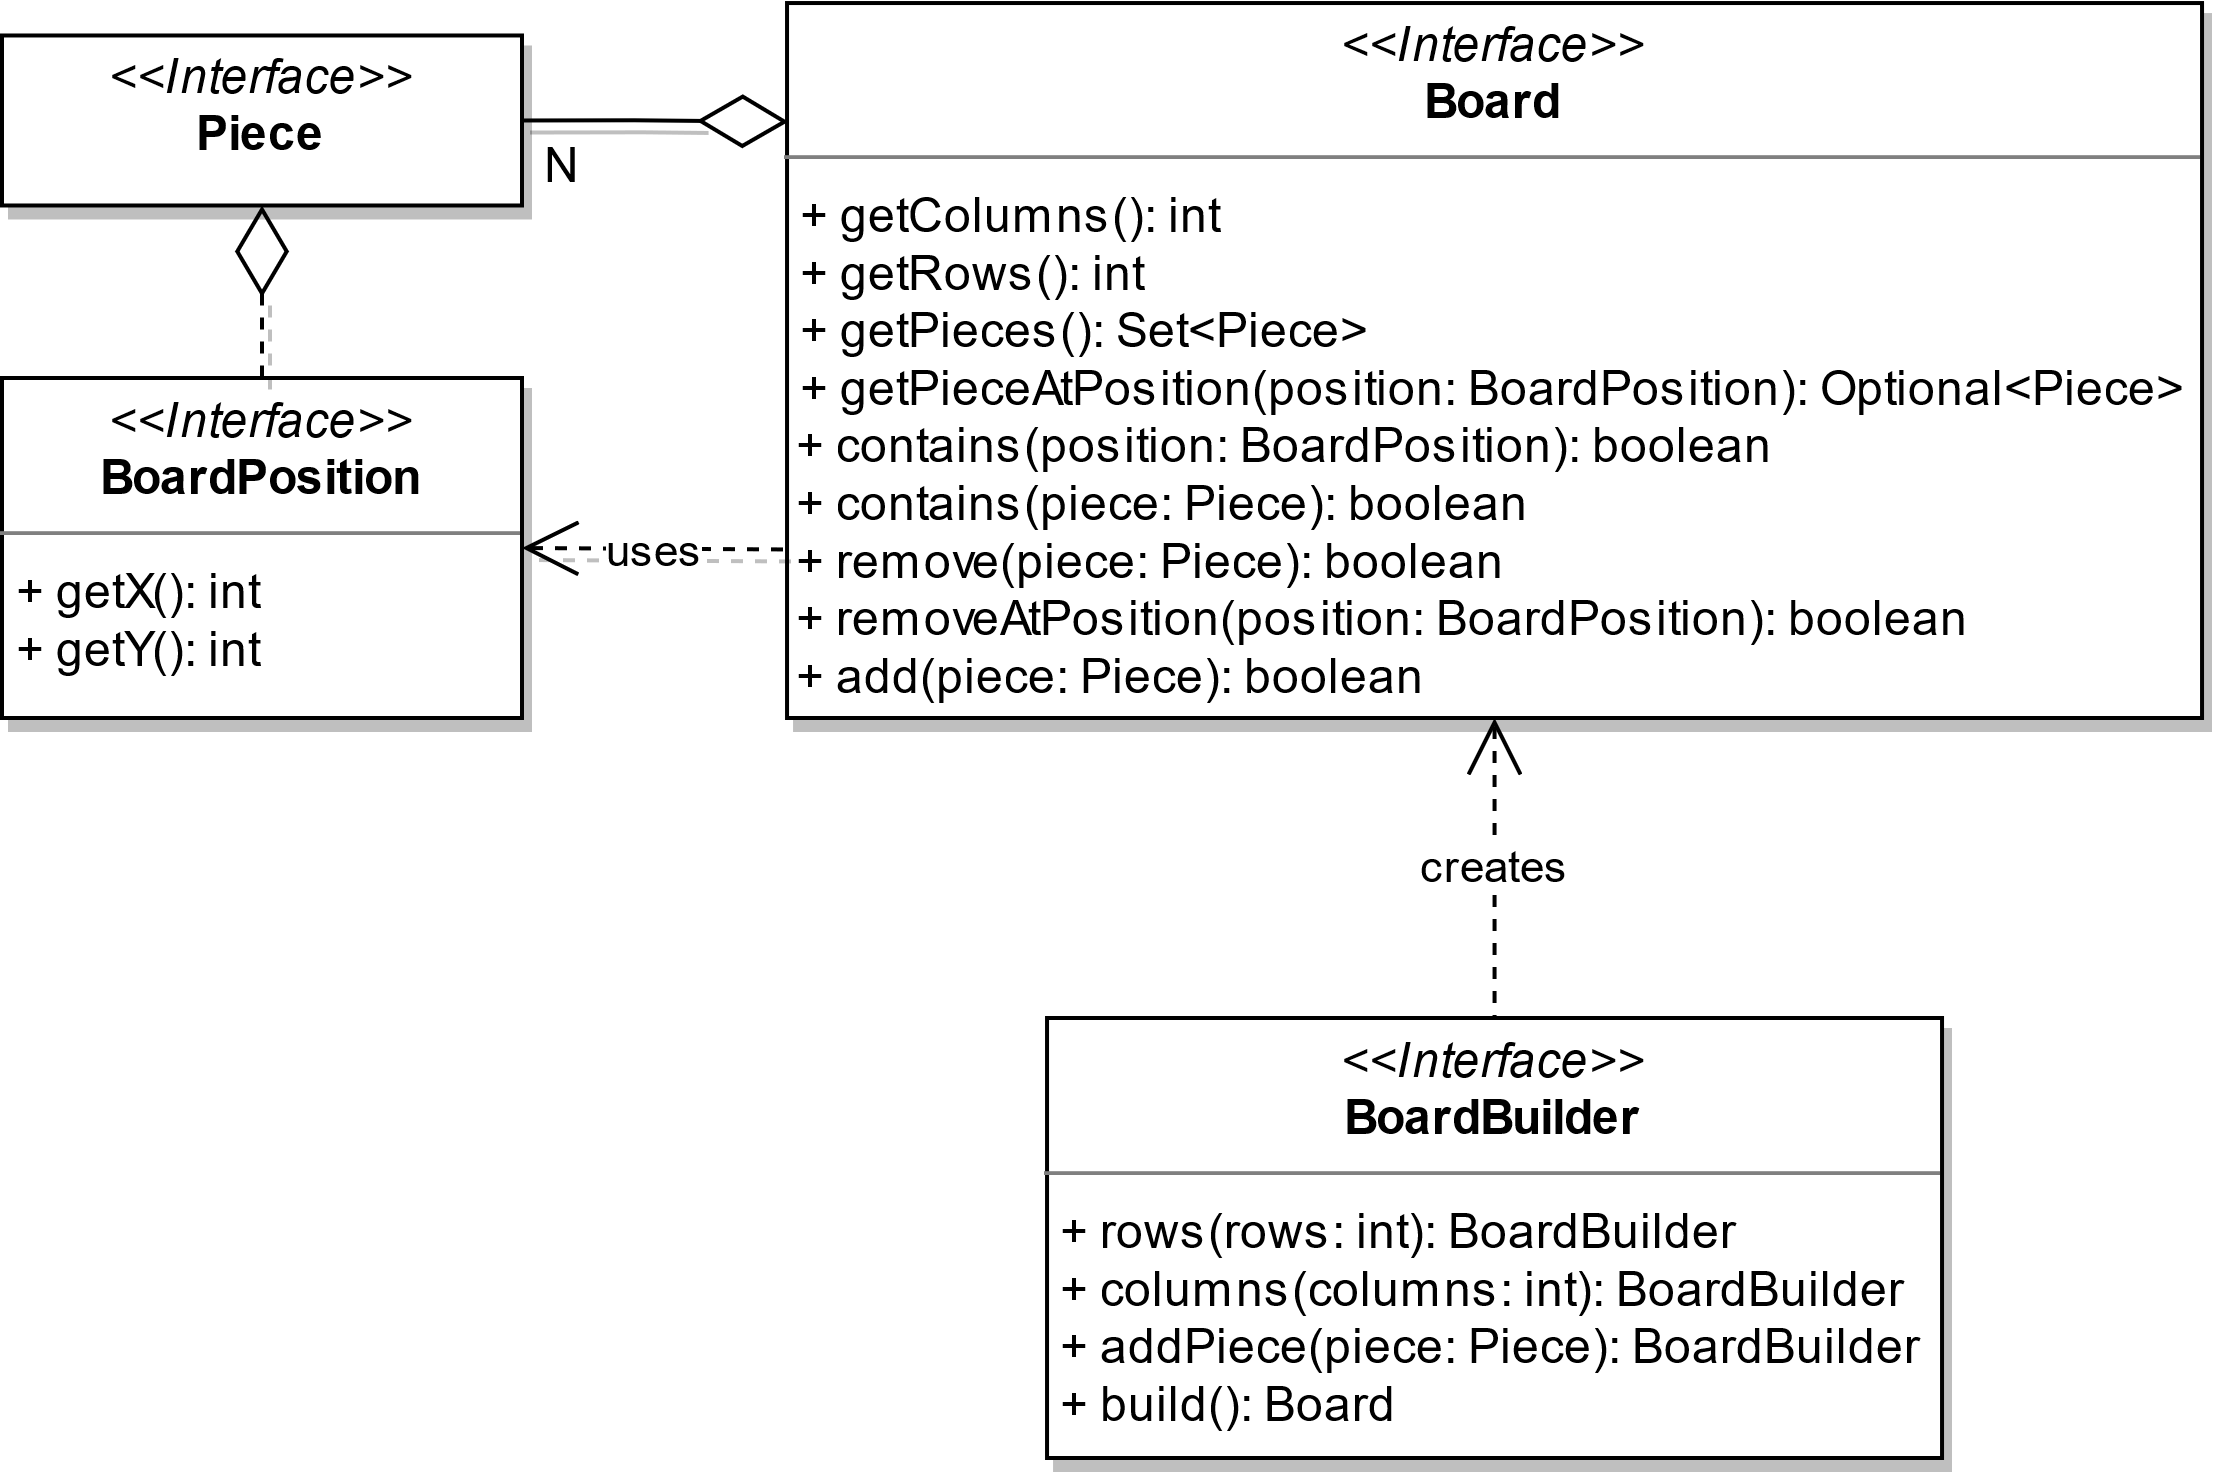
\includegraphics[scale=0.9]{img/Stefano/Board.png}
    \end{center}
    \caption{Focus gestione scacchiera}
    \label{img:Board}
\end{figure}
%

\chapter{Sviluppo}
\section{Testing automatizzato}

Sin dalle fasi iniziali abbiamo deciso di approcciarci allo sviluppo seguendo una metodologia test-driven, utilizzando JUnit 5.
\\
I test venivano scritti in modo tale cercare di "rompere" l'applicativo, così facendo siamo stati in grado di scovare problemi ed errori altrimenti difficilmente individuabili.
\\
Come principio, nel caso un test non passasse, ci si soffermava ad individuare il problema per poi risolverlo. Non venivano aggiunte feature e non si proseguiva con lo sviluppo fino a che i test non passassero tutti.\\
Alla creazione di una feature, oppure di una sezione dell'applicativo, venivano creati i relativi test.
\\
Soprattutto nelle fasi iniziali, dove c'era necessità di studiare gli edge-cases ed il funzionamento del motore, non avendo ancora implementato la GUI, i test sono risultati il modo più efficace e veloce per scovare inconsistenze altrimenti quasi impossibili da identificare. In più, quando implementata, è anche stato testato il funzionamento corretto della GUI.


\subsection{Andruccioli Manuel}
Avendo realizzato qualche componente che va a scrivere su file, ho deciso fosse corretto testare il tutto. Infatti, nei test, viene salvata una copia dei dati già esistenti, in modo da poterla ripristinare alla fine degli stessi.
\\
Avendo sviluppato lo scheletro della scacchiera grafica, ho pensato fosse corretto che venisse testata ed ho sfruttato la libreria \href{https://github.com/TestFX/TestFX}{\texttt{TestFX}}.
\\
Una prima parte è servita per testare le funzionalità basilari dell'applicazione.
\\
Un test importante che ho realizzato è stato quello di \texttt{integration}: viene simulata un'intera partita di scacchi in modo random. Questo test ci ha permesso di scovare un bug che altrimenti non avremmo trovato facilmente: su \texttt{Windows} non dava problemi, mentre su \texttt{Linux}, dopo molte mosse, il gestore dei suoni dava errore e non faceva più crearne.

\begin{itemize}
    \item UserTest
    \item UserBuilderTest
    \item UserStorageTest
    \item UserManagerTest
    \item ValidatorTest
    \item LeaderboardTest
    \item GameBoardTest
    \item \textbf{Integration}: GameBoardIntegrationTest
\end{itemize}

\subsection{Scolari Stefano, Mazzoli Alessandro}
Avendo sviluppato componenti dell'applicativo che per essere testate nella loro interezza necessitavano di un certo grado di mutualità, abbiamo deciso di collaborare a stretto contatto per la loro realizzazione.\\
Sarebbe sinceramente difficile dividere con rigore quali test siano stati sviluppati con assoluta indipendenza uno dall'altro e per questo abbiamo scelto di citarli come test comuni.\\
Le componenti sono state testate in parallelo al loro sviluppo.
\\
Il motore è stato strutturato in maniera \texttt{layered}, test di componenti successive andavano ad utilizzare componenti precedentemente già testate, garantendone la correttezza.
Si nota infatti dai test, un progressivo grado di astrazione: partendo inizialmente dal poter testare semplicemente se un pezzo modificasse la propria posizione, fino al simulare situazioni di gioco, testandone il corretto \texttt{outcome}.
Così facendo siamo arrivati ad analizzare anche il corretto funzionamento di alcune delle varianti implementate.
\begin{itemize}
    \item MovementTest
    \item MovementManagerTest
    \item ClassicGameControllerTest
    \item PawnMovementVariantTest
    \item PieceSwappingVariantTest
    \item PieceTest
    \item BoardTest
    \item MatchTurnsTest
    \item ClassicGameTypeMatchTest
\end{itemize}

\subsection{Patriti Tommaso}
Testare la mia parte è stato fondamentale, infatti, dovendo lavorare con risorse del jar e file, le eccezioni e variabili di cui controllare integrità e correttezza sono state molteplici.
Il test riguardante il \texttt{Timer}, è particolare, in quanto utilizza una sleep per verificarne il funzionamento.
\begin{itemize}
    \item TimerTest
    \item SettingTest
    \item ReplayTest
    \item DynamicConfigTest

\end{itemize}

\section{Metodologia di lavoro}

Sviluppando il progetto si è cercato di mantenere più indipendenza possibile dal punto di vista del lavoro svolto, pur sempre confrontandoci quotidianamente per aggiornare l'un l'altro dei progressi fatti sulle rispettive sezioni di lavoro.
\\
La fase iniziale è stata di analisi, durante la quale abbiamo lavorato tutti e quattro a stretto contatto per definire attraverso grafici UML ed idee quella che doveva essere la nostra architettura.
\\
Ci siamo soffermati per molte ore su questa fase, ed infatti l'implementazione concreta di quello che avevamo ideato e definito è risultato privo di particolari inghippi o problemi.
\\
Durante le fasi iniziali di sviluppo la collaborazione e confronto è stata molto intensa.
\\
Proseguendo con lo sviluppo ogni componente del gruppo ha lavorato con indipendenza alla propria parte.

\subsubsection{Workflow}
Per organizzare bene il workflow di gruppo sul progetto abbiamo utilizzato Trello.com, dove nella bacheca da noi creata era possibile definire degli "step" e delle indicazioni su quali fossero le cose da gestire o implementare, il tutto seguendo un ordine gerarchico. 
Per ottenere ciò ci siamo basati sul \textbf{metodo KanBan} che prevede di avere 3 colonne:
\begin{itemize}
    \item \textbf{To-Do}: l'insieme delle cosa da fare non ancora iniziate.
    \item \textbf{Doing}: l'insieme delle cosa che si stanno implementando.
    \item \textbf{Done}: l'insieme delle cose già completate.
\end{itemize}
In questo modo con Trello abbiamo gestito la creazione di Task che qualcuno avrebbe dovuto svolgere, infatti una volta creato un task lo si poteva assegnare ad uno o più persone.
Avendo la colonna dei Doing si poteva sempre sapere chi stava lavorando a cosa evitando di finire a lavorare in parallelo alla stessa cosa.
\
\\
La nostra estensione del KanBan prevedeva altre colonne quali \textbf{Bug Fix} e \textbf{General}, in BugFix venivano spostati tutti i Task completati ma che andavano controllati mentre su General c'erano gli appunti e le idee che venivano in mente ai membri del gruppo per migliorare il progetto.

\subsubsection{Version Control}
Come DVCS è stato utilizzato Git.
\\
Si è scelto di utilizzare una metodologia ispirata a GitFlow, dove il branch principale era 'main', dal quale sono state fatte le release.
\\
Il branch di sviluppo di default è stato 'develop'.
\\
Nel momento in cui vi era la necessità di sviluppare una nuova feature, si creava ogni volta un branch apposito denominato 'feature-*', nel quale si aveva quindi la possibilità di implementare la funzionalità in un ambiente separato, senza rischiare di avere "collisioni" con il lavoro di altri membri del gruppo.
\\
I vari componenti del gruppo hanno quindi lavorato sui branch delle feature in quel momento da loro sviluppate, per poi mergiare il tutto, una volta passati i test, sul branch 'develop'.

\subsection{Andruccioli Manuel}
Realizzazione dell'intero sotto-sistema di salvataggio degli utenti con i loro rispettivi punteggi e possibilità di recuperarli, sotto forma di classifica. Funzionalità per validare la password degli utenti.
\\
Creazione dell'utility per generare la cartella \texttt{.jhaturanga} nella home directory e controlli su di essa. Successivamente è stata ampliata da chi aveva necessità di aggiungere file al suo interno.
\\
Realizzazione dello scheletro grafico della scacchiera con possibilità di drag-and-drop dei pezzi. Realizzazione della grafica relativa alla classifica. Caching di immagini e suoni.

\subsection{Mazzoli Alessandro}
Realizzazione del motore scacchistico: gestione ed implementazione del concetto di  \texttt{Game} e di \texttt{Match}.
\\
Sviluppo dei componenti quali il \texttt{Player} ed implementazione della modalità online tramite MQTT.
\\
Refactoring della grafica dell'applicazione e delle board della GUI tramite la struttura gerarchica delle \texttt{GraphicBoard}.
\\
Gestione generale della struttura MVC.


\subsection{Patriti Tommaso}
Grafica volta al test dell'applicazione durante le prime fasi di sviluppo con fxml di base, timer e chiamate asincrone, salvataggio e replay delle partite, suoni della scacchiera, pezzi scacchiera personalizzabili, grafica applicazione personalizzabile, possibilità di poter installare dei resource pack esterni, salvataggio delle impostazioni preferite dall'utente e relativa gestione file json, binding dell'applicazione(resizable), struttura ramificata dei css e caricamento di questi ultimi, PageLoader per caricamento, switch, reload e passaggio della scena, gestione di alcune directory di .jhaturanga.

\subsection{Scolari Stefano}
Realizzazione del motore scacchistico: gestione ed implementazione \texttt{GameController}, implementazione movimenti e \texttt{MovementManager}, creazione strategie di movimento.\\
Implementazione ed ideazioni delle varianti e realizzazione dei problemi scacchistici.\\
Gestione \texttt{Piece} e \texttt{Board} iniziali.\\
Implementazione controller relativi a sezioni affini a quelle da me sviluppate ed implementazione grafica iniziale delle \texttt{Board} utilizzando \texttt{JavaFx}.

\section{Note di sviluppo}

\subsection{Andruccioli Manuel}
\begin{itemize}
\item \textbf{Programmazione Funzionale} durante lo sviluppo, soprattutto per la validazione delle password.

\item \textbf{Optional} molto presenti in gran parte del mio codice, proprio per evitare null come valore di ritorno. Sono stati molto utili per aggiungere chiarezza al codice.

\item \textbf{Generici}: sfruttati per definire un'interfaccia utile alla creazione di funzioni.

\item \textbf{GSON}: libreria utilizzata per il salvataggio degli utenti su file Json.

\item \textbf{Google Guava}: libreria utilizzata per l'Hashing delle password.

\item \textbf{TestFX}: libreria utilizzata per il testing dell'interfaccia grafica.
\end{itemize}

\subsection{Mazzoli Alessandro}
\begin{itemize}

\item \textbf{Programmazione Funzionale} durante lo sviluppo di questo progetto ho potuto sfruttarla per quel che è inerente alla gestione del motore scacchistico. 
È risultato infatti di inimitabile aiuto il package java.util.function che ho avuto modo di approfondire durante il progredire del progetto.

\item \textbf{Lambda} di paro passo con la programmazione funzionale è risultato necessario se non obbligatorio a livello stilistico utilizzare le lambda expression, le quali mi hanno permesso di avere del codice pulito, leggibile e chiaro.

\item \textbf{Stream} ampiamente utilizzate di paro passo con quella che è stata la parte che fa uso della programmazione funzionale e delle lambda expression.
\\
Le ho trovate una delle feature più interessanti che Java offre e tuttora me le sto studiando sempre più nel profondo per capire come funzionano internamente.
\\
Per comprenderne ancora di più l'utilizzo ne ho inoltre creata un implementazione in Python creando una libreria.

\item \textbf{Optional} data l'estrema utilità e flessibilità ne ho utilizzati molti nella mia parte di model. Ho notato che offrono una gran chiarezza nella gestione di possibili valori nulli e inoltre offrono metodi che permettono di sfruttare la programmazione funzionale quali map, orElse, ifPresent...

\item \textbf{MQTT} avendo implementato la modalità online tramite protocollo MQTT è stato di fondamentale aiuto l'utilizzo della libreria paho-mqtt che mi ha permesso di implementare la comunicazione via internet molto velocemente.

\item \textbf{Gradle} fin dall'inizio mi sono occupato del setup del progetto che fin da subito è stato deciso che sarebbe stato gestito tramite gradle. Durante il periodo di sviluppo ho avuto modo di approfondire, seppur poco, il suo funzionamente poichè lo trovo uno strumento molto potente e assolutamente indispensabile in un progetto dove si ha bisogno di librerie esterne. È risultato infatti di estrema facilità l'importazione di librerie tramite Gradle.

\end{itemize}

\subsection{Patriti Tommaso}
\begin{itemize}
\item \textbf{JavaFx} è stato il motore grafico della nostra applicazione, e ho tenuto molto a gestire la flessibilità grafica. Ogni pagina ha il suo personale file fxml e per mezzo dei binding l'applicazione si adatta a qualunque monitor desktop, mantenendo una continuità grafica in tutti i sistemi operativi.(In OSX e alcuni linux Desktop manager il full screen viene gestito in maniera particolare e ho lavorato per avere un PageLoader in grado di gestire ogni variante)
\item \textbf{Gson}, libreria di google per la gestione di file json, è stata necessaria per la gestione dei file di configurazione dell'applicazione.
\item \textbf{Reflections} è stata utilizzata per navigare agevolmente nelle risorse del file jar e poter duplicare dei file di default.
\item \textbf{Optional} Nella mia parte di progetto ho lavorato con molti file, quindi per la gestione di eventuali file non presenti o per errori di formattazione, è stato obbligatorio l'utilizzo di Optional.
\item \textbf{I tipi generici} sono stati utili per avere un' implementazione efficace di Strategy.
\item \textbf{Runnable} sono stati utili per avere una comunicazione asincrona con l'applicazione senza side-effect generati dall'implementazione dei Thread da parte delle view.
\item lambda e stream usate dove necessario
\end{itemize}

\subsection{Scolari Stefano}
\begin{itemize}
\item \textbf{Stream} Scrivere \texttt{Stream} ed utilizzarle nelle mie sezioni di progetto è stata una tra le parti che ho apprezzato maggiormente, a tal punto che ho deciso in alcune specifiche parti di utilizzare una libreria esterna chiamata "StreamEx", che nasce come "enhancement" delle \texttt{Stream} classiche fornite da Java.
\\
Avendo lavorato principalmente alla sezione del motore scacchistico, interfacciarmi con \texttt{Collection} oppure necessitarne la creazione era una costante. 
\\
Le \texttt{Stream} sono quindi risultate utilissime, ed infatti sono presenti in quasi tutte le classi da me scritte.
\item \textbf{Generici} Perché il package \texttt{java.util.function} non fornisce una \texttt{TriFunction}, ho avuto necessità di scrivere una semplice \texttt{Functional Interface} che utilizza quindi i generici, lo stesso vale per il \texttt{TriPredicate}.
\item \textbf{Lambda expressions} Ho fatto largo uso delle lambda expressions, sia quando trattavo le Stream, sia quando dovevo definire ed utilizzare interfacce funzionali. Ho anche cercato di utilizzare il \textbf{Method Reference} ove possibile.
\item \textbf{Programmazione funzionale} Pur non avendo affrontato questo argomento a lezione, durante le fasi di sviluppo ho avuto modo di imparare strada facendo ed utilizzare ampiamente il package \texttt{java.util.function} e le rispettive interfacce funzionali.
Ho in molti punti definito \texttt{Predicate}, \texttt{BiPredicate}, \texttt{Supplier}, \texttt{Consumer}, \texttt{Function} e \texttt{UnaryOperator}, infatti le strategie di movimento dei pezzi, alla base, ne fanno largo uso.
\item \textbf{Optional} Ho utilizzato molto spesso \texttt{Optional} ed i metodi di questa classe (map, orElseGet, etc) quando vi era la necessità di lavorare con valori potenzialmente nulli.
\end{itemize}

\subsection{Crediti}
\begin{itemize}
    \item \textbf{Page} L'idea dell'entità \texttt{Page} è stata ispirata dalla classe \href{https://bitbucket.org/danysk/oop17-burattini-samuele-ciarafoni-nicholas-dente-francesco/src/master/src/oopang/view/GameScene.java}{\textbf{\texttt{GameScene}}} del progetto OOPang
    \item \textbf{PageLoader} L'idea del componente \texttt{PageLoader} è ispirata dalla classe (\href{https://bitbucket.org/danysk/oop17-burattini-samuele-ciarafoni-nicholas-dente-francesco/src/master/src/oopang/view/javafx/SceneLoader.java}{\textbf{\texttt{SceneLoader}}} del progetto OOPang.
\end{itemize}
\chapter{Commenti finali}

\section{Autovalutazione e lavori futuri}

\subsection{Andruccioli Manuel}

Sono molto soddisfatto del lavoro svolto, sia da me, che dal mio team. Fin dalle fasi di analisi, abbiamo avuto grande capacità comunicativa, esponendo i nostri dubbi, pensieri e motivazioni. Questa armonia nel gruppo ha generato un flusso di lavoro ottimale per procedere nella realizzazione del progetto.
\\
Seppur non abbia partecipato alla logica del motore scacchistico, proprio perché non sarebbe stato possibile dividerci quella parte in 4, mi sono ritagliato una modesta sezione, dove ho gestito, sempre in ottica di estensibilità, la possibilità di salvare gli utenti e i suoi relativi dati.
\\
L'utilizzo corretto di \texttt{Git}, ci ha permesso un lavoro agile, pensando ognuno alla sua parte, per poi unirle insieme una volta terminato lo sviluppo. Questo ciclo di vita ci ha permesso di incrementare gradualmente le funzionalità.
\\
Questa metodologia di lavoro mi ha permesso di comprendere le difficoltà dei progetti di dimensione maggiore a ciò che si può/riesce a vedere in aula.
\\
Ringrazio il mio team per il lavoro svolto.

\subsection{Mazzoli Alessandro}
Fin dall'inizio mi sono occupato della gestione architetturale del progetto a livello della struttura dei package, costruita in moda da avere una gerarchia in modo che sia molto semplice trovare una interfaccia/classe quando se ne ha bisogno.
\\
Questo è stato fatto fin dall'inizio in vista di un possibile incremento molto elevato del numero di classi, come infatti è successo.
\\
Ci si è ritrovati infatti alla fine con un elevato numero di classi che tuttavia però era agevolmente gestibile poiché avevamo una solida gerarchia dei package.
\paragraph{}
\
\\
Essendo io un appassionato di Clean Code un altro aspetto molto importante in cui ho aiutato è stata consigliare i miei compagni sulle "regole" da seguire in modo da avere un progetto e un codice pulito e uniforme. 
\\
Durante tutta la parte di sviluppo dell'applicazione ho utilizzato ampiamente la tecnica del refactoring, riguardando il codice da me scritto e le scelte da me fatte analizzandole criticamente e cercando di capire in che modo si potesse migliorare l'architettura da me creata. 
\\
Questo ha portato ad un continuo refactor che mi ha permesso di rendere la mia parte di codice a mio parere molto esplicativa e ben strutturata.
\\
Molto di aiuto in questa fase è stato l'utilizzo del plugin CheckStyle che ho trovato di estrema utilità nella creazione di software pulito ed uniforme.
\\
Parte fondamentale è stato il continuo utilizzo di UML che mi ha aiutato ad avere una visione d'insieme del contesto sui cui stavo lavorando in modo da poter ad esempio scomporre un'entità più grossa in un insieme di più entità di dimensione inferiore.
\\
Altro tool fondamentale è stato l'utilizzo di Git, che ho avuto di modo di imparare ad usare abbastanza bene.
Tuttavia spero in futuro di poterlo studiare più a fondo potendone utilizzare le feature più avanzate che a non ci sono state insegnate a lezione.
\\
Durante lo sviluppo del progetto Jhaturanga ho avuto modo di venire sempre di più a contatto con quello che è il mondo della programmazione funzionale da cui sono rimasto affascinato.
\\
Spero di avere modo di approfondirla ulteriormente studiandola insieme alla Reactive Programming poiché le trovo altamente entusiasmanti e interessanti.

\subsection{Patriti Tommaso}
Questa attività è stata importante per la mia crescita, soprattutto dal punto di vista progettuale. Purtroppo sono entrato nel vivo dell'analisi del progetto in un secondo momento rispetto ai miei compagni, e questo nella fasi intermedie di sviluppo ha determinato scarsa produttività  nelle parti più interne(model). Nelle fasi finali sono riuscito a dedicarmi al progetto in maniera più concreta, una volta fatta un' ulteriore analisi delle mie parti, sono andato a sistemare e correggere il codice scritto in precedenza e a gestire in maniera più efficiente le ultime funzionalità da me aggiunte, integrandole bene con il lavoro svolto dai miei colleghi.
\\
Sinceramente non sono pienamente soddisfatto del mio operato, un mio maggior coinvolgimento nelle parti iniziali di progettazione e studio dei Pattern avrebbe sicuramente portato il mio lavoro ad un gradino più alto, anche se credo di aver avuto un buon incremento qualitativo nelle ultime fasi del progetto.
\\
Un aspetto molto positivo è stato un buon utilizzo di \texttt{Git}, che usavo già da diverso tempo ma in maniera inappropriata.
\\
Per quanto riguarda il lavoro d’equipe, la comunicazione all’ interno del gruppo è stata serena e lineare, anche per merito di numerose sessioni d'esame affrontate già precedentemente assieme che ci hanno permesso di trovare un ottimo grado di affiatamento e collaborazione.
\\
Per il futuro conto di continuare a studiare in maniera approfondita la programmazione ad oggetti, integrandola possibilmente con nuovi linguaggi.

\subsection{Scolari Stefano}
Lavorare a questo progetto mi ha permesso di affinare maggiormente le mie conoscenze di Java e di approccio allo sviluppo. 
\\
Prima di sviluppare questo applicativo mi era totalmente estraneo come gestire un progetto di tali dimensioni lavorando in team.
\\
Mi ritengo molto soddisfatto del lavoro svolto e delle nuove competenze acquisite. Sono molto felice della comunicazione e della generale gestione del lavoro da parte del gruppo.
\\
Ritengo di essermi impegnato molto per la buona riuscita di questo progetto, ho cercato di adottare le metodologie di lavoro migliori possibili ed ho sempre tentato di scrivere codice al massimo delle mie capacità.
\\
Come citato nella sezione precedente, durante lo sviluppo ho avuto modo di approcciarmi, se pur a livello basico, ad alcuni concetti ed aspetti della programmazione funzionale che mi sono risultati utili per scrivere più agilmente il codice.
\\
Il mio obiettivo per il futuro è approfondire diversi aspetti della programmazione ad oggetti, studiando in maniera ancora più profonda quali siano le good-practice di Java, le tecniche di sviluppo e l'uso dei Pattern.
\\
Durante le fasi di sviluppo mi sono appassionato a queste tematiche, leggendo molto a riguardo e guardando diversi talk sull'argomento(e.g.: Devoxx Talk).
\\
Sono inoltre molto curioso di conoscere meglio il mondo della programmazione funzionale.


\section{Difficoltà incontrate e commenti per i docenti}

\subsection{Andruccioli Manuel}

Ritengo indubbiamente che questo sia uno dei migliori corsi mai frequentati finora. La sua completezza, profondità, precisione, mi ha portato ad acquisire qualità non da poco.
\\
Il fatto che non sia riuscito a superare l'esame al primo tentativo, mi ha portato a passare due settimane intere sulla programmazione funzionale, il che è stato davvero importante per acquisire, in modo non superficiale, competenze utili sia in Java, ma anche in altri ambiti. Tornando su progetti personali (e.g. che utilizzano Javascript), ho potuto subito apprezzare l'utilizzo della programmazione funzionale.
\\
Ringrazio i professori per la qualità e l'impegno speso per la realizzazione di questo corso.

\subsection{Mazzoli Alessandro}
Sono stato molto soddisfatto dalle conoscenze appreso dal corso di Programmazione Ad Oggetti, lo reputo assolutamente il corso più valido visto finora.
\\
Di grande importanza è stata la capacità di spiegazione dei docenti sia di teoria che di laboratorio che si sono rivelati essere di un eccellente preparazione riuscendo a rispondere a qualsiasi mio dubbi anche se questo andava molto nello specifico.
\\
L'apprendimento è risultato quindi semplice e gradevole dato l'elevata qualità delle spiegazioni fornite che miravano ad estirpare qualsiasi dubbio degli studenti.
\\
Inoltre una nota di merito va al fatto che vengano insegnati i Design Pattern, e si cerca inoltre di far passare agli studenti un po di enfasi verso l'arte del clean code.
\paragraph{}
\
\\
Le uniche pecche che ho potuto trovare sono state forse la spiegazione di JavaFx e di Gradle.
\\
Entrambi questi argomenti sono stati spiegati a lezione, tuttavia JavaFX è stata trattato molto velocemente senza particolari approfondimenti, quindi per sviluppare il progetto è stato necessario studiarne il funzionamento in autonomia.
\\
Tuttavia il cercare l'indipendenza degli studenti nello studiarsi un framework la trovo un ottima pratica per prepararli a quello che sarà poi il mondo del lavoro.
\paragraph{}
\
\\
Relativamente a Gradle, che ho trovato un po' più complesso da studiarsi rispetto a JavaFx, l'unica nota che vorrei segnalare è che la spiegazione di questo tool viene fatta verso metà anno, quando purtroppo gli studenti non sono ancora nell'ottica del progetto.
\\
Reputo quindi che sarebbe stato meglio farne una spiegazione leggermente più approfondita verso fine del corso, enfatizzandone l'importanza nel progetto e mostrando qualche esempio di utilizzo più avanzato.

\subsection{Patriti Tommaso}
A mio avviso questo è stato il corso più serio affrontato fino ad ora. Per me è stato molto importante in quanto è andato a spaziare vari aspetti della programmazione e mi ha fatto vedere quest'ultima con una luce differente, nel bene e nel male. Questo corso, i laboratori e soprattutto il progetto svolto con i miei compagni sono stati dei tasselli importanti che sicuramente mi hanno aiutato a capire quale strada voler prendere nella giungla dell'informatica.
\\
Probabilmente il maggior scoglio da me affrontato è stato quello di applicare le buone regole del "clean code" e perdere le cattive abitudini.  


\subsection{Scolari Stefano}
Quello di Programmazione ad Oggetti è stato il corso che ho seguito con maggior interesse e che maggiormente mi ha appassionato.
\\
Le lezioni tenute durante il corso sono sempre state chiare e precise. L' attenzione, professionalità e nitidezza con cui il professor Viroli ha tenuto il corso, mi ha in qualche modo spinto a cercare di dare il massimo sia durante l'esame sia lavorando al progetto.
\\
Questo corso è l'unico fino ad ora che mi ha portato a voler approfondire e studiare indipendentemente temi legati alla materia, andando oltre quello che mi era stato spiegato a lezione.
\\
L'utilizzo di Pattern, il dare importanza alla "qualità" del software sviluppato, le tecniche avanzate del linguaggio, i principi di buona programmazione, le metodologie di approccio al lavoro e di sviluppo sono tutti temi che voglio approfondire, sia individualmente che accademicamente.


\appendix

\chapter{Guida utente}

\section{Selezione Piattaforma}
All'avvio dell'applicazione, lanciando il comando 'java -jar nomeJar.jar', verrà chiesto all'utente di scegliere attraverso quale piattaforma grafica interagire con il software, terminale oppure GUI.

\begin{figure}[H]
    \begin{center}
        \centering
        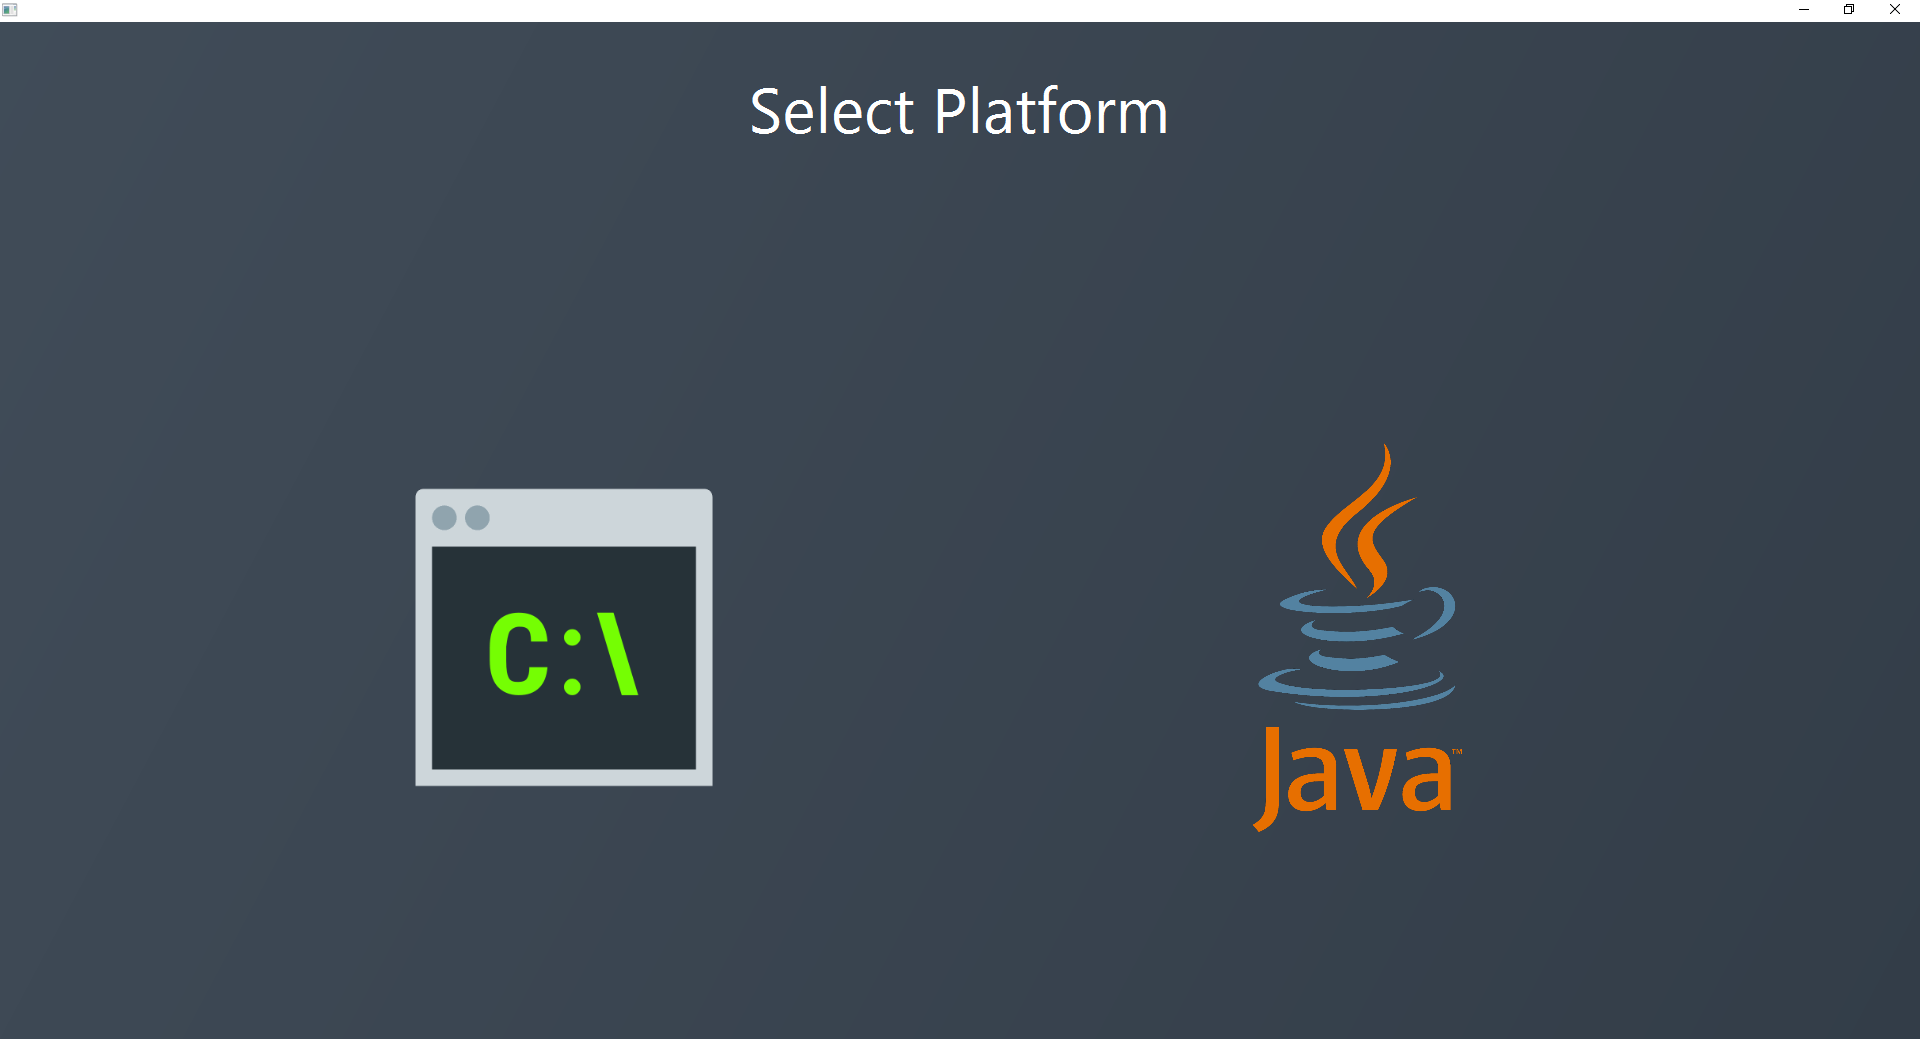
\includegraphics[scale=0.3]{img/guidaUtente/avvioJhaturanga.png}
    \end{center}
    \caption{Schermata iniziale per scelta piattaforma grafica}
    \label{img:avvioJhaturanga}
\end{figure}

%
\
\\
Poiché la versione da riga di comando è un semplice proof-of-concept, come precedentemente detto, non rappresenta l'applicativo nella sua interezza, ed è quindi meno fornita di opzioni e feature rispetto alla controparte da GUI.
\\
Anche per questo motivo non ci si è occupati di rendere portabile la versione da terminale, sfortunatamente infatti non è possibile visualizzare nè da CMD nè da Powershell i caratteri rappresentanti i simboli degli scacchi.
\\
Se si vuole comunque testare l'applicativo nella sua versione command-line da Windows sarà necessario settare la console in modo tale da supportare i colori ed un font che contenga i simboli dei pezzi degli scacchi.
\\
Per settare correttamente la console:

\begin{itemize}
    \item Si segua questa soluzione per abilitare la visualizzazione dei colori da Powershell e CMD \url{https://stackoverflow.com/a/51681675/13800588}
    \item Si segua poi invece questa guida per aggiungere un nuovo font(si consiglia DejaVu Sans)
    \url{https://maketecheasier.com/add-custom-fonts-command-prompt-windows10/}
\end{itemize}
\
\\
Ci concentreremo ora a guidare l'utente nell'uso della versione GUI, in quanto quella da command-line risulta essere intuitiva.


\section{Login}
Una volta scelta la modalità di gioco da GUI verrà richiesto di eseguire il login, oppure la registrazione. Nel caso non si sia interessati a registrarsi e tenere traccia dei punti si può saltare questo passaggio premendo il pulsante 'Log as Guest'.
\begin{figure}[H]
    \begin{center}
        \centering
        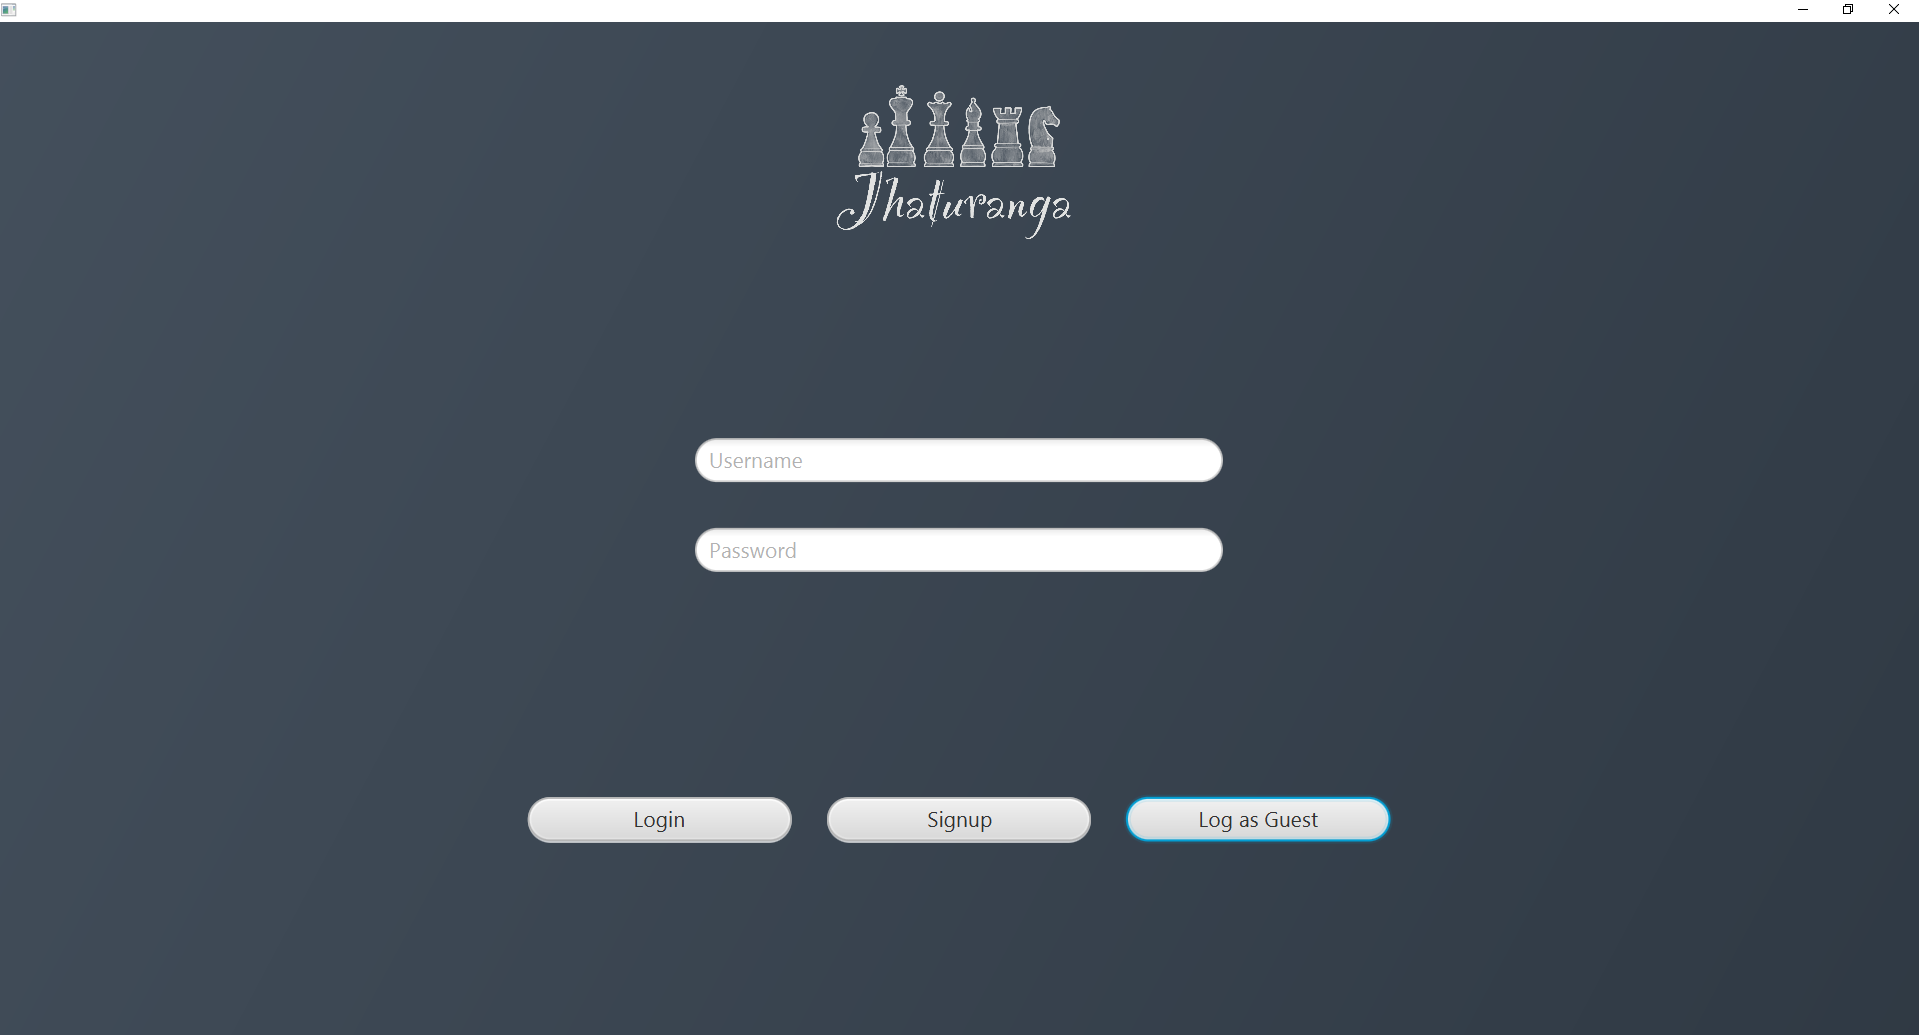
\includegraphics[scale=0.25]{img/guidaUtente/login.png}
    \end{center}
    \caption{Schermata di login}
    \label{img:login}
\end{figure}

%
\section{Home Page}
Superata la schermata di login ci si troverà nella sezione principale dell'applicativo, da cui è possibile iniziare una nuova partita, visualizzare la leaderboard, visualizzare i replay delle partite giocate oppure accedere alle impostazioni.
\\
Inoltre in alto a destra saranno presente gli username dei due utenti loggati, di default il secondo user è un guest.
Per cambiare utente basterà cliccare sulla label corrispettiva e si aprirà la pagina di login.
\begin{figure}[H]
    \begin{center}
        \centering
        \includegraphics[scale=0.25]{img/guidaUtente/sceltaModalità.png}
    \end{center}
    \caption{Schermata selezione modalità}
    \label{img:sceltaModalità}
\end{figure}


\section{Settings}
Dalla pagina delle impostazioni sarà possibile cambiare i vari stili dell'applicazione tra i quali:
\begin{itemize}
    \item Tema dell'applicazione
    \item Stile dei pezzi
    \item Volume dell'applicazione
\end{itemize}
\begin{figure}[H]
    \begin{center}
        \centering
        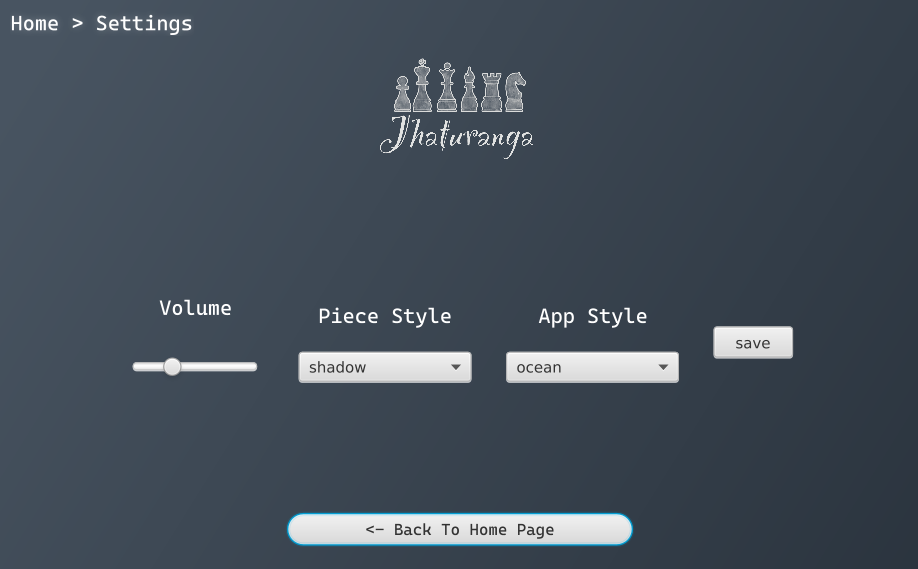
\includegraphics[scale=0.4]{img/guidaUtente/settings.png}
    \end{center}
    \caption{Schermata selezione modalità}
    \label{img:guidaSettings}
\end{figure}

\section{Leaderboard}
Dalla pagina della leaderboard sarà possibile visualizzare la classifica degli utenti salvati.
\\
Cliccando sulle varie header tab tipo "Wins" e "Loses" si potrà ordinare gli utenti in ordine crescente/descrescente relativamente a quel carattere. 
\begin{figure}[H]
    \begin{center}
        \centering
        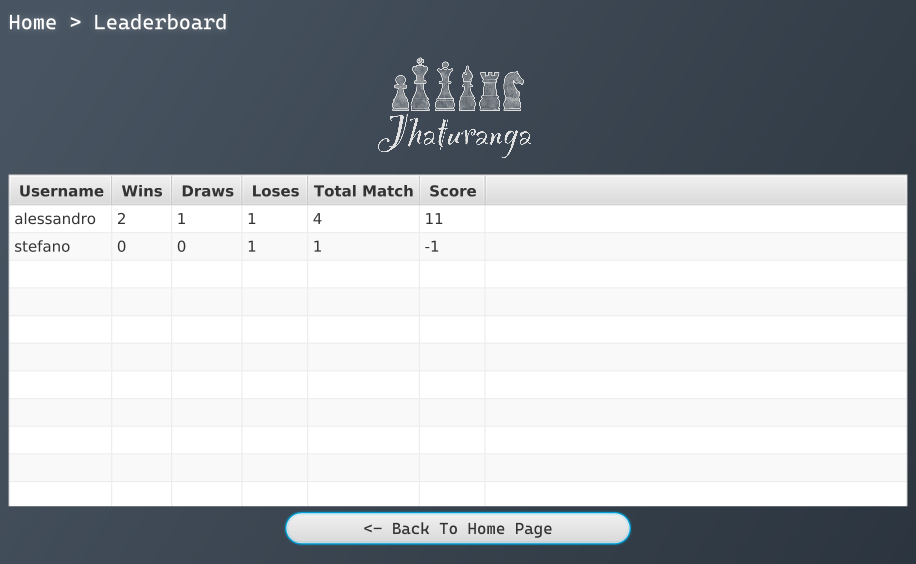
\includegraphics[scale=0.4]{img/guidaUtente/leaderboard.png}
    \end{center}
    \caption{Schermata selezione modalità}
    \label{img:leaderboard}
\end{figure}

\section{History}
Dalla pagina History sarà possibile visualizzare l'elenco delle partite salvate e sceglierne una di cui visualizzare il replay.
Una volta cliccato il bottone per visualizzarlo si aprirà quindi la pagina in cui verrà avviata la partita.
Per navigare all'interno dello storico delle mosse si utilizzino i tasti analoghi a quelli utilizzati in-game che verrano spiegati nel capitolo dell'interfaccia di gioco.
\begin{figure}[H]
    \begin{center}
        \centering
        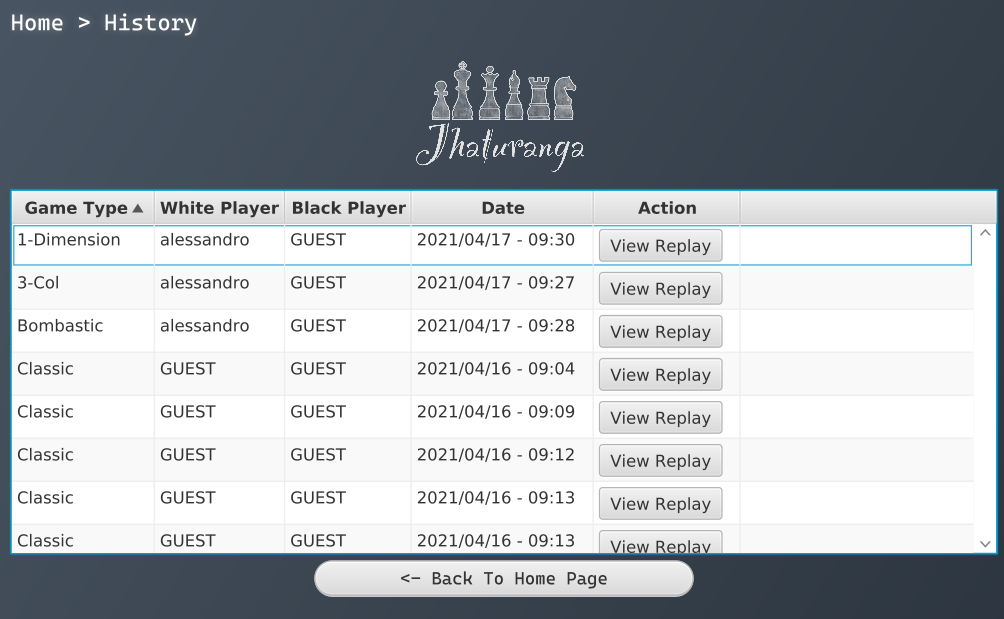
\includegraphics[scale=0.4]{img/guidaUtente/guidaHistory.png}
    \end{center}
    \caption{Schermata selezione modalità}
    \label{img:guidaHistory}
\end{figure}

\section{Nuova Partita}
Nel caso si voglia iniziare una nuova partita verrà chiesto all'utente se la si vuole giocare in locale oppure online.

\begin{figure}[H]
    \begin{center}
        \centering
        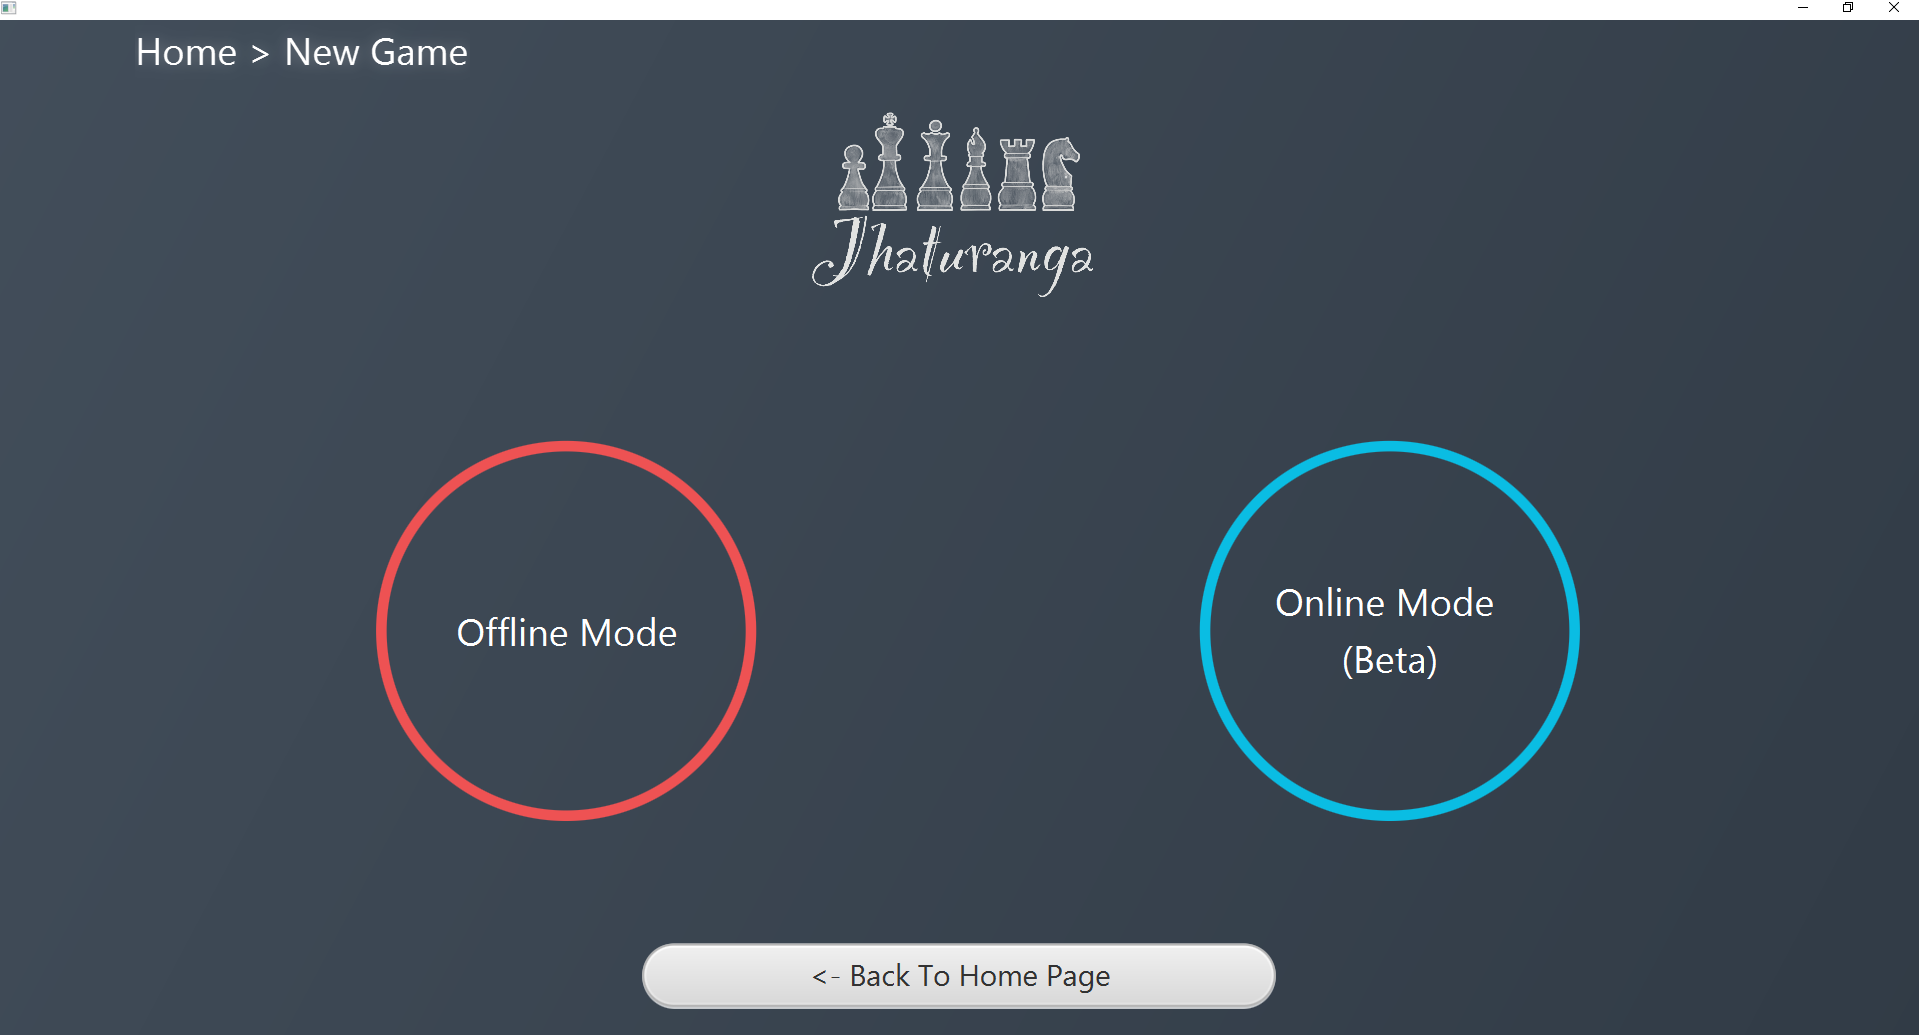
\includegraphics[scale=0.25]{img/guidaUtente/onlineOffline.png}
    \end{center}
    \caption{Selezione offline oppure online}
    \label{img:onlineOffline}
\end{figure}


\section{Modalità Online}
Nel caso la si giochi online si potrà scegliere se creare una partita oppure se unirsi ad una partita attraverso un codice.
Se si sceglie di crearne una si viene inviati alla pagina di selezione della modalità di gioco e una volta cliccato il bottone \textbf{Play} dopo qualche secondo comparirà un popup con il codice del Match che andrà fatto inserire al giocatore che si vuole unire alla partita.
\begin{figure}[H]
    \begin{center}
        \centering
        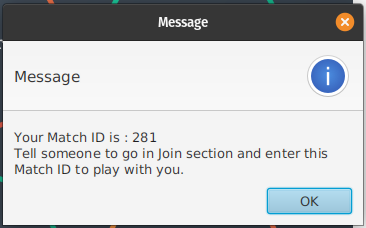
\includegraphics[scale=0.75]{img/guidaUtente/online_create_popup.png}
    \end{center}
    \caption{Schermata selezione modalità}
    \label{img:online_popup}
\end{figure}

\section{Modalità Offline}
Se invece si vuole giocare offline saranno presenti tre opzioni: la select game type, la customized board e la chess problems.

\begin{figure}[H]
    \begin{center}
        \centering
        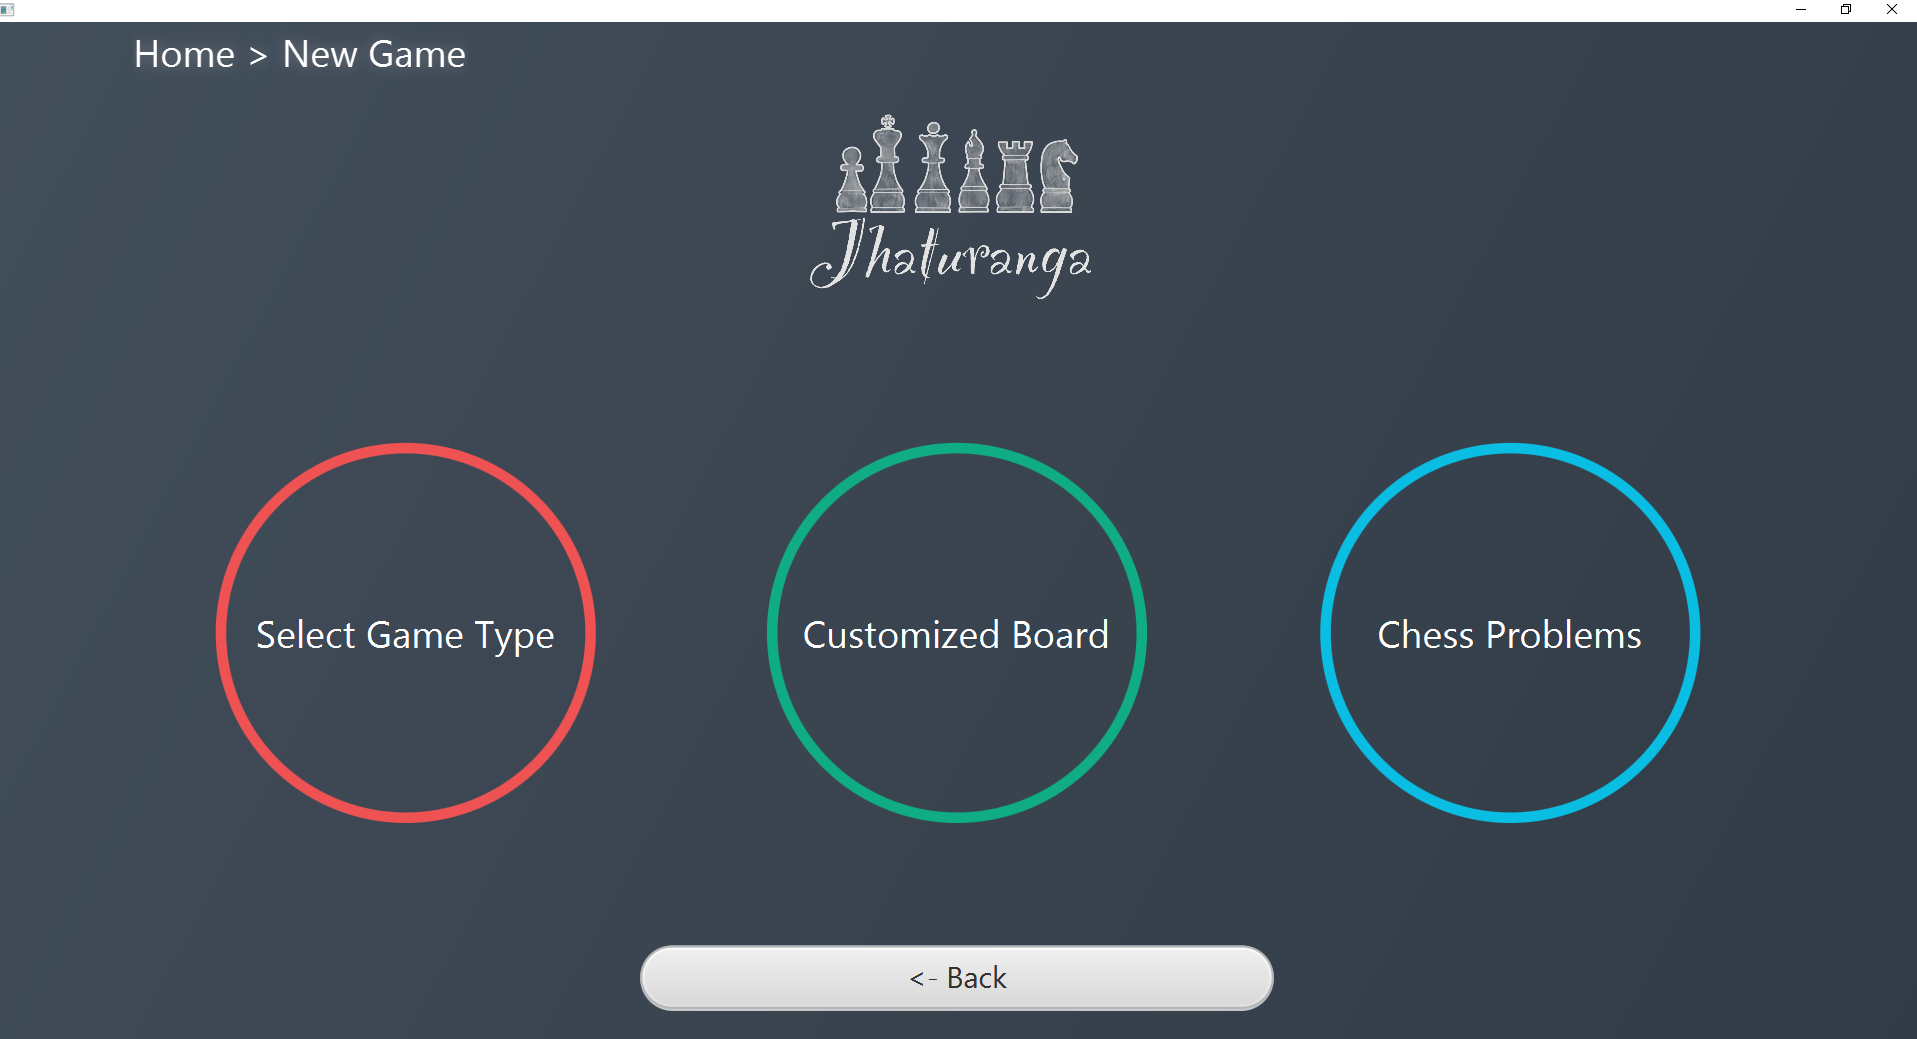
\includegraphics[scale=0.25]{img/guidaUtente/sottomenuSelezine.png}
    \end{center}
    \caption{Menù selezione game type}
    \label{img:sottomenuSelezine}
\end{figure}

%
\section{Selezione Modalità}
Dalla prima è possibile selezionare una delle molte varianti scacchistiche.
Si usi la rotella del mouse per navigare fra le varie modalità.
\\
Nella tab di destra è possibile selezionare il timer da utilizzare per la partita ed a chi assegnare il colore bianco.
\\
Una volta premuto su play inizierà la partita.

\begin{figure}[H]
    \begin{center}
        \centering
        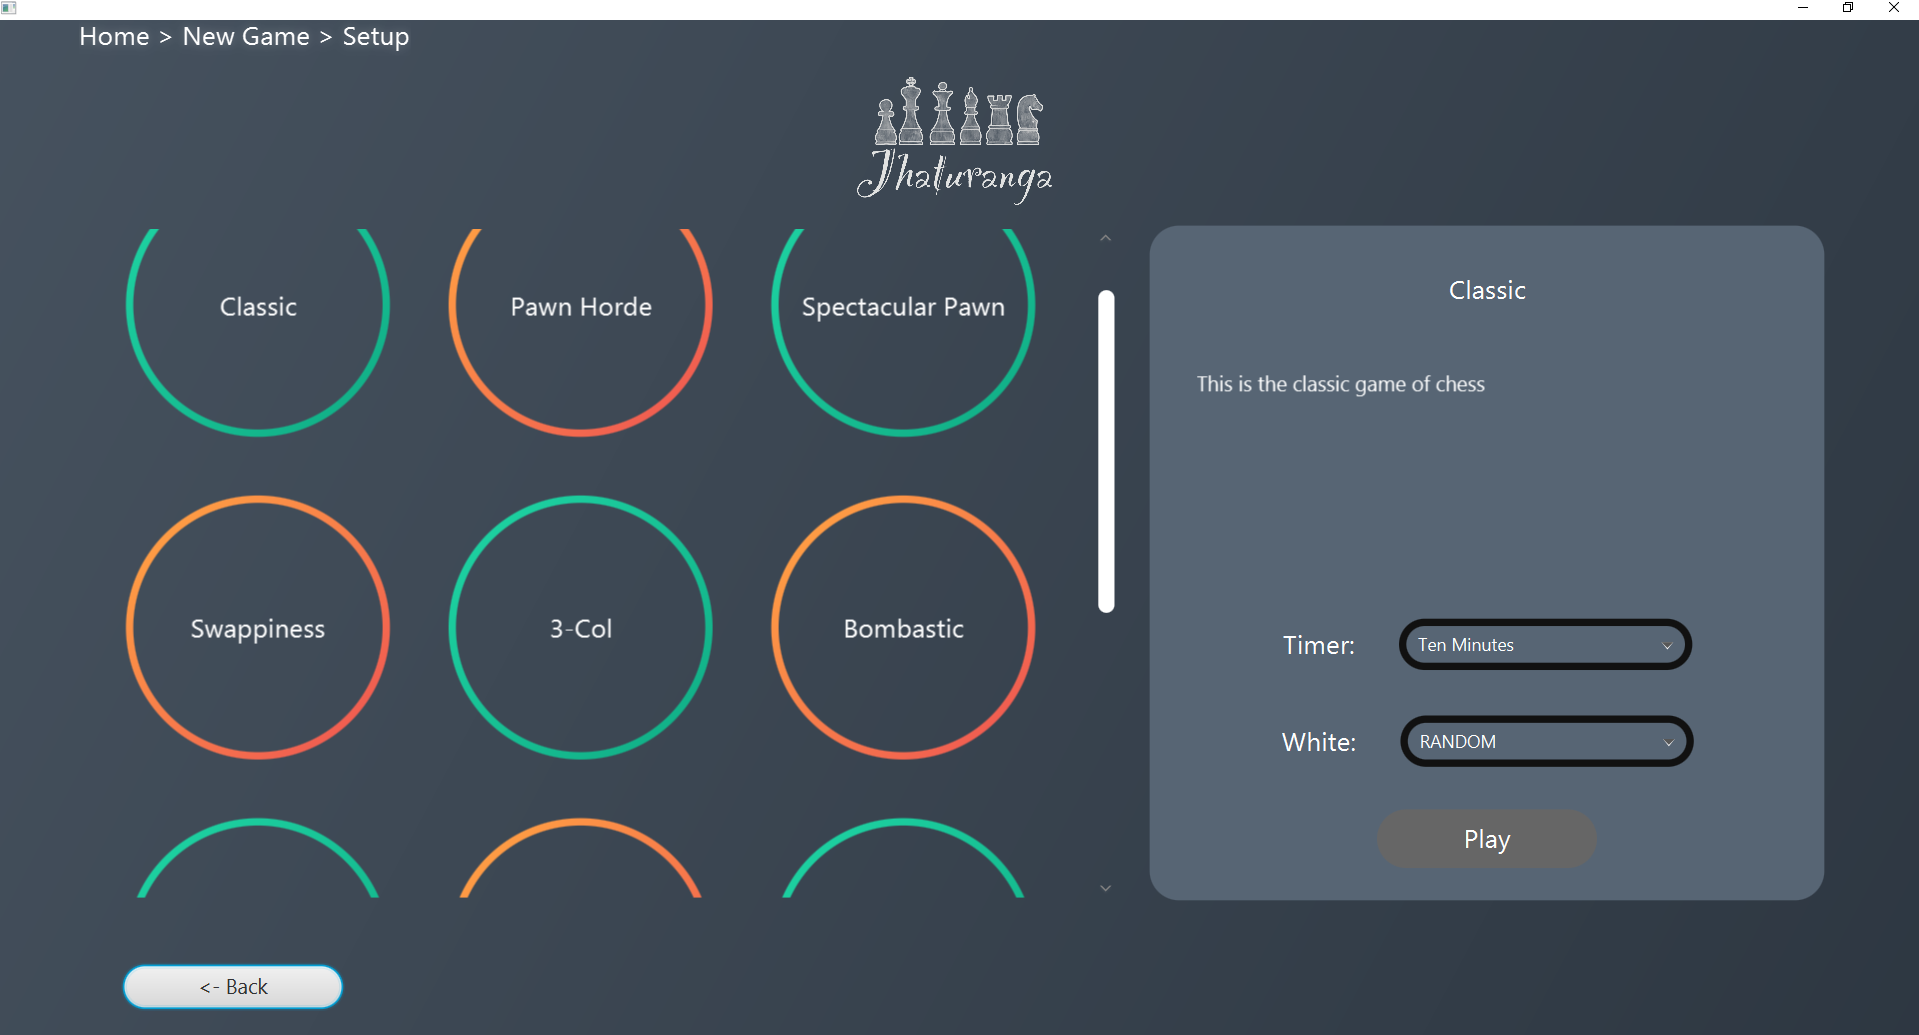
\includegraphics[scale=0.25]{img/guidaUtente/selezioneGameType.png}
    \end{center}
    \caption{Selezione del game type}
    \label{img:selezioneGameType}
\end{figure}
\
%
\section{Interfaccia Di Gioco}
L'interfaccia di gioco si presenta nel seguente modo, il giocatore bianco si trova nella posizione bassa della scacchiera ed ha il rispettivo username + timer in basso a sinistra, il giocatore nero invece si troverà nella parte alta della scacchiera con il rispettivo username + timer in alto a destra.
\paragraph{}
\
\\
Cliccando su un pezzo ci viene mostrato dove quel pezzo si può muovere marchiando le posizione valide.
\\
Per muovere i pezzi serve trascinarli e rilasciarli nella posizione di destinazione.
\\
Una volta effettuata una mossa questa rimarrà evidenziata tramite la colorazione della cella di partenza e quella di arrivo fino a che il giocatore avversario non farà la sua mossa.
\paragraph{}
\
\\
Mentre si gioca è possibile visualizzare lo storico delle mosse, muovendosi avanti(tasto "D" oppure "->") ed indietro(tasto "A", oppure "<-").
\\
Con in tasto "resign" è possibile arrendersi e terminare la partita.
\begin{figure}[H]
    \begin{center}
        \centering
        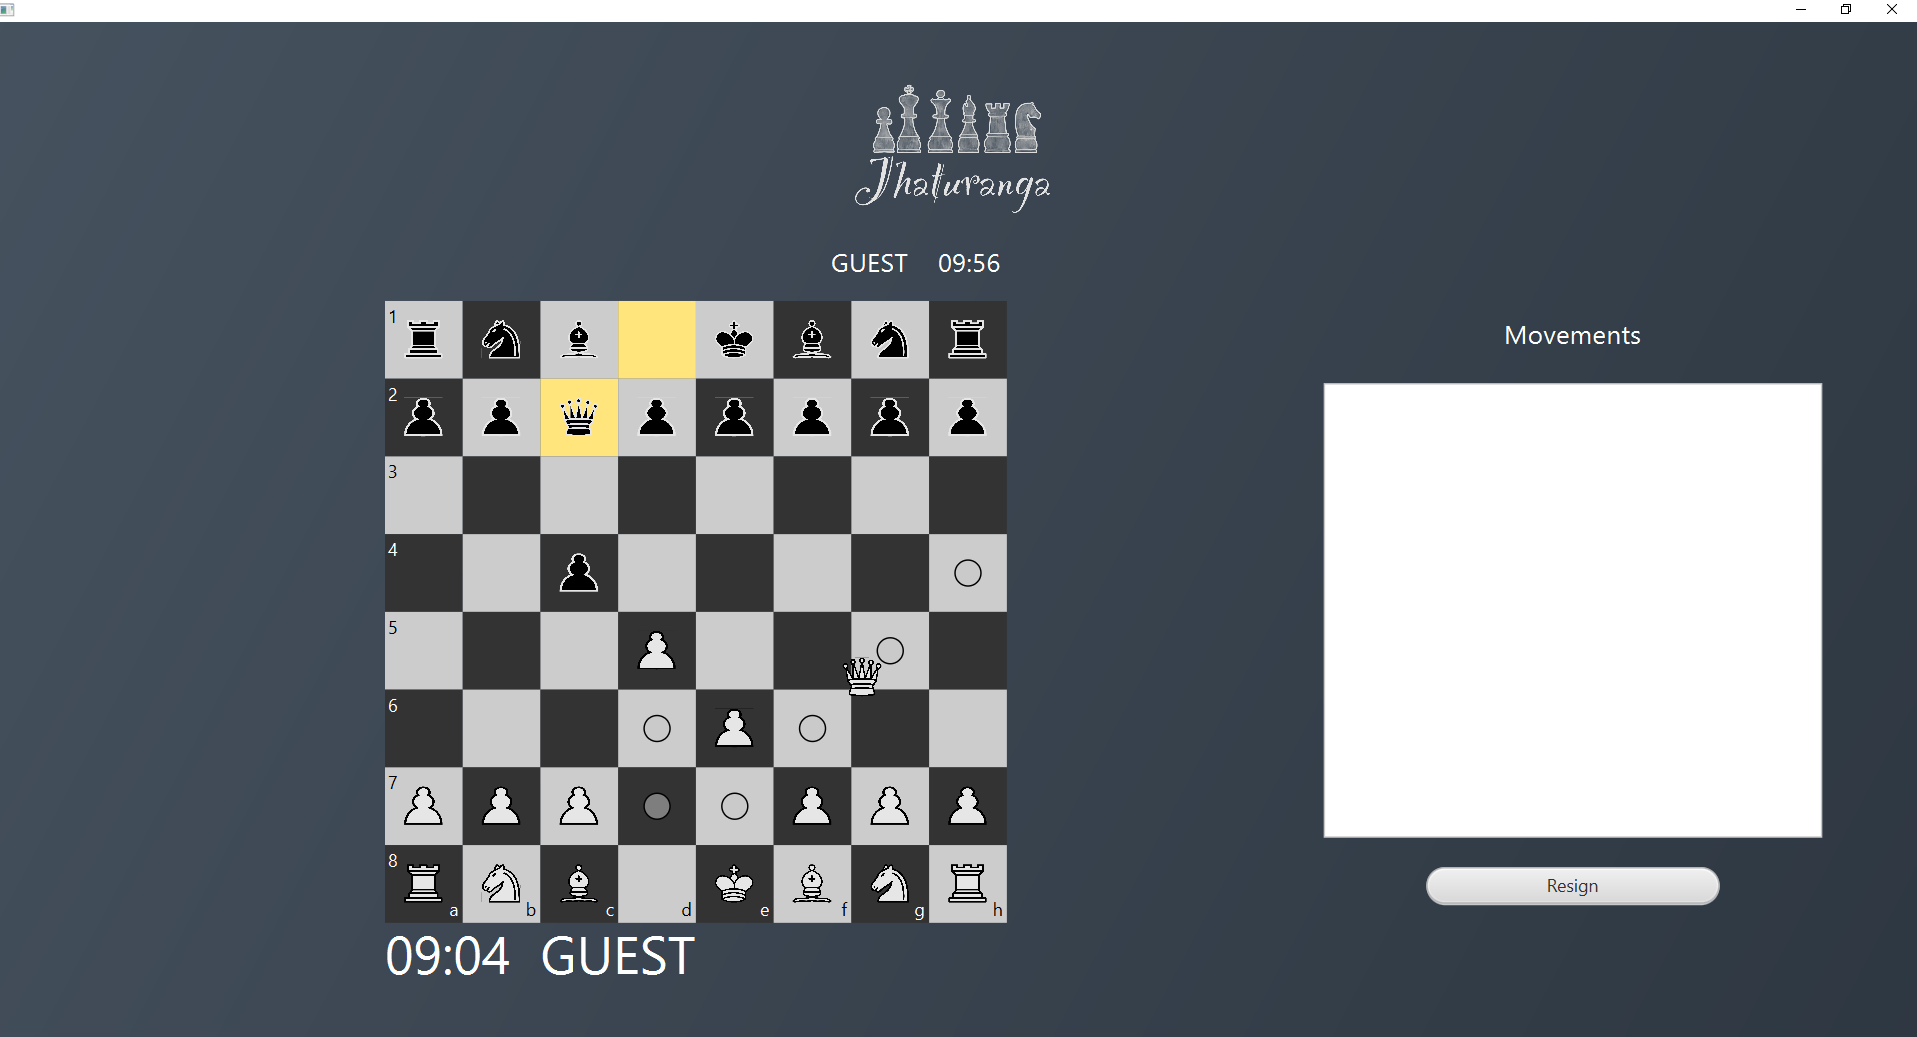
\includegraphics[scale=0.25]{img/guidaUtente/schermataDiGioco.png}
    \end{center}
    \caption{Schermata di gioco}
    \label{img:schermataDiGioco}
\end{figure}

\section{Scacchiera Personalizzata}
Dalla seconda invece si apre una board editor per creare la propria scacchiera di partenza customizzata. Le dimensioni della scacchiera sono ridimensionabili tramite i due prompt per inserire il numero di righe e colonne ed il tasto "resize" per applicare le modifiche.
I pezzi vanno trascinati dalla sezione di destra e rilasciati sulla board tramite il LMB. Per rendere più veloce l'aggiunta dello stesso pezzo è possibile tenere premuto CTRL mentre si trascina un pezzo per "disegnare" la tastiera di quel pezzo.\\
Per rimuovere pezzi si utilizzi il tasto destro, sia cliccando individualmente sulla casella interessata, sia tenendo premuto mentre si trascina.\\
Una volta che si decide di aver ultimato la creazione della propria board si prema il tasto "Start" per iniziare la partita che utilizzerà la scacchiera appena creata come board di partenza.

\begin{figure}[H]
    \begin{center}
        \centering
        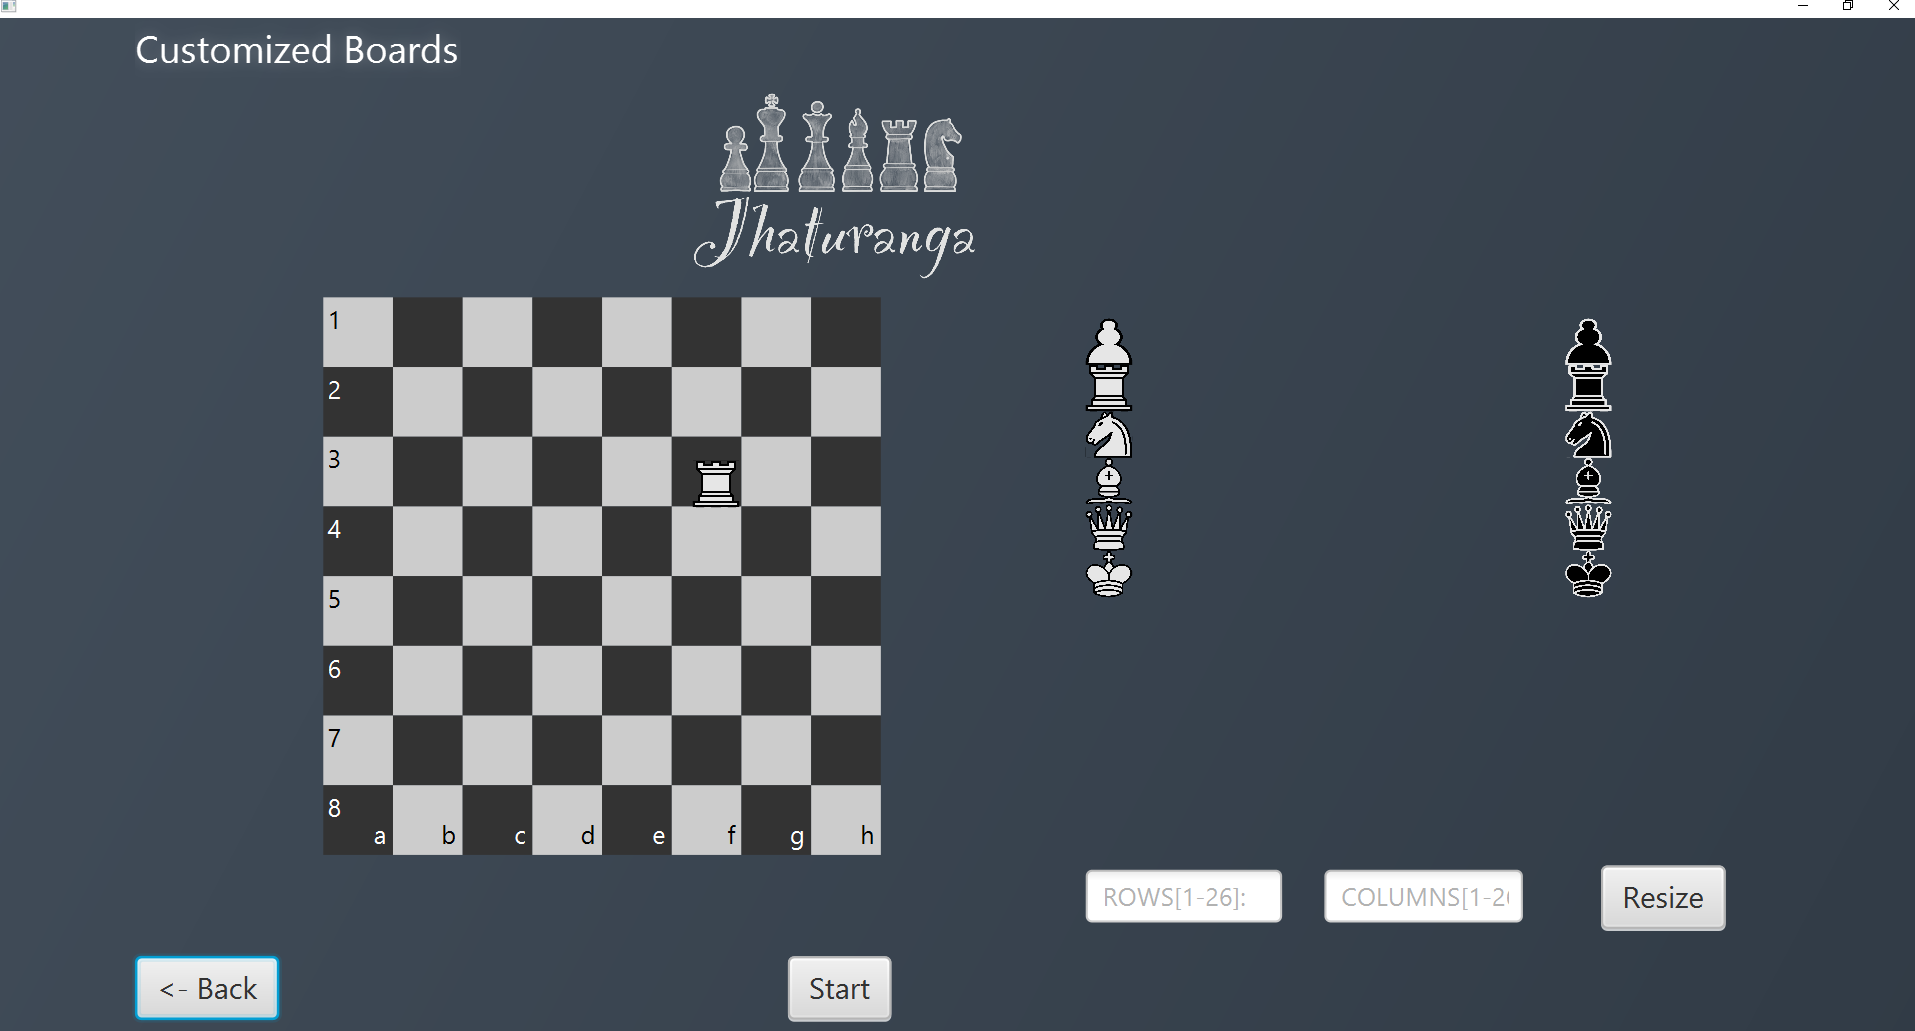
\includegraphics[scale=0.25]{img/guidaUtente/editorBoard.png}
    \end{center}
    \caption{Schermata per l'editing della board}
    \label{img:editorBoard}
\end{figure}

\section{Problemi Scacchistici}
La sezione per i problemi scacchistici risulta analoga a quella per la selezione dei game type.

\section{Resource Pack}
Per aggiungere uno stile all'applicazione è possibile aggiungere figlio di stile (css) nella cartella .jhaturanga situata nella home directory. Più precisamente il file andrà aggiunto nella sottodirectory res/css/themes.
Per aggiungere invece uno stile concernente la grafica dei pezzi, bisogna aggiungere una cartella contenente le immagini di questi ultimi nella sottodirectory res/pieces.
Andrà seguito il pattern degli stili gia presenti seguendone quindi la denomenclatura e il formato dei file.

\chapter{Esercitazioni di laboratorio}

\section{Andruccioli Manuel}

\begin{itemize}
 \item Laboratorio 04: \url{https://virtuale.unibo.it/mod/forum/discuss.php?d=62685#p101058}
 \item Laboratorio 05: \url{https://virtuale.unibo.it/mod/forum/discuss.php?d=62684#p101061}
 \item Laboratorio 06: \url{https://virtuale.unibo.it/mod/forum/discuss.php?d=62579#p100885}
 \item Laboratorio 07: \url{https://virtuale.unibo.it/mod/forum/discuss.php?d=62582#p100887}
 \item Laboratorio 08: \url{https://virtuale.unibo.it/mod/forum/discuss.php?d=63865#p102770}
 \item Laboratorio 09: \url{https://virtuale.unibo.it/mod/forum/discuss.php?d=64639#p103801}
 \item Laboratorio 10: \url{https://virtuale.unibo.it/mod/forum/discuss.php?d=66753#p106682}
 \item Laboratorio 11: \url{https://virtuale.unibo.it/mod/forum/discuss.php?d=66463#p106435}
\end{itemize}

\section{Mazzoli Alessandro}

\begin{itemize}
 \item Laboratorio 05: \url{https://virtuale.unibo.it/mod/forum/discuss.php?d=62684#p101104}
 \item Laboratorio 06: \url{https://virtuale.unibo.it/mod/forum/discuss.php?d=62579#p100892}
 \item Laboratorio 07: \url{https://virtuale.unibo.it/mod/forum/discuss.php?d=62582#p100894}
 \item Laboratorio 08: \url{https://virtuale.unibo.it/mod/forum/discuss.php?d=63865#p102831}
 \item Laboratorio 09: \url{https://virtuale.unibo.it/mod/forum/discuss.php?d=64639#p104182}
 \item Laboratorio 10: \url{https://virtuale.unibo.it/mod/forum/discuss.php?d=66753#p106622}
 \item Laboratorio 11: \url{https://virtuale.unibo.it/mod/forum/discuss.php?d=66463#p106266}
\end{itemize}



\section{Patriti Tommaso}

\begin{itemize}
 \item Laboratorio 06: \url{https://virtuale.unibo.it/mod/forum/discuss.php?d=62579#p101540}
 \item Laboratorio 07: \url{https://virtuale.unibo.it/mod/forum/discuss.php?d=62582#p101567}
 \item Laboratorio 08: \url{https://virtuale.unibo.it/mod/forum/discuss.php?d=63865#p103917}
 \item Laboratorio 09: \url{https://virtuale.unibo.it/mod/forum/discuss.php?d=64639#p104080}
\end{itemize}


\section{Scolari Stefano}

\begin{itemize}
 \item Laboratorio 04: \url{https://virtuale.unibo.it/mod/forum/discuss.php?d=62685#p101107}
 \item Laboratorio 05: \url{https://virtuale.unibo.it/mod/forum/discuss.php?d=62684#p101105}
 \item Laboratorio 06: \url{https://virtuale.unibo.it/mod/forum/discuss.php?d=62579#p101037}
 \item Laboratorio 07: \url{https://virtuale.unibo.it/mod/forum/discuss.php?d=62582#p100910}
 \item Laboratorio 08: \url{https://virtuale.unibo.it/mod/forum/discuss.php?d=63865#p102771}
 \item Laboratorio 09: \url{https://virtuale.unibo.it/mod/forum/discuss.php?d=64639#p103968}
 \item Laboratorio 10: \url{https://virtuale.unibo.it/mod/forum/discuss.php?d=66753#p106627}
\end{itemize}

\end{document}
